\documentclass[twoside]{book}

% Packages required by doxygen
\usepackage{fixltx2e}
\usepackage{calc}
\usepackage{doxygen}
\usepackage[export]{adjustbox} % also loads graphicx
\usepackage{graphicx}
\usepackage[utf8]{inputenc}
\usepackage{makeidx}
\usepackage{multicol}
\usepackage{multirow}
\PassOptionsToPackage{warn}{textcomp}
\usepackage{textcomp}
\usepackage[nointegrals]{wasysym}
\usepackage[table]{xcolor}

% Font selection
\usepackage[T1]{fontenc}
\usepackage[scaled=.90]{helvet}
\usepackage{courier}
\usepackage{amssymb}
\usepackage{sectsty}
\renewcommand{\familydefault}{\sfdefault}
\allsectionsfont{%
  \fontseries{bc}\selectfont%
  \color{darkgray}%
}
\renewcommand{\DoxyLabelFont}{%
  \fontseries{bc}\selectfont%
  \color{darkgray}%
}
\newcommand{\+}{\discretionary{\mbox{\scriptsize$\hookleftarrow$}}{}{}}

% Page & text layout
\usepackage{geometry}
\geometry{%
  a4paper,%
  top=2.5cm,%
  bottom=2.5cm,%
  left=2.5cm,%
  right=2.5cm%
}
\tolerance=750
\hfuzz=15pt
\hbadness=750
\setlength{\emergencystretch}{15pt}
\setlength{\parindent}{0cm}
\setlength{\parskip}{3ex plus 2ex minus 2ex}
\makeatletter
\renewcommand{\paragraph}{%
  \@startsection{paragraph}{4}{0ex}{-1.0ex}{1.0ex}{%
    \normalfont\normalsize\bfseries\SS@parafont%
  }%
}
\renewcommand{\subparagraph}{%
  \@startsection{subparagraph}{5}{0ex}{-1.0ex}{1.0ex}{%
    \normalfont\normalsize\bfseries\SS@subparafont%
  }%
}
\makeatother

% Headers & footers
\usepackage{fancyhdr}
\pagestyle{fancyplain}
\fancyhead[LE]{\fancyplain{}{\bfseries\thepage}}
\fancyhead[CE]{\fancyplain{}{}}
\fancyhead[RE]{\fancyplain{}{\bfseries\leftmark}}
\fancyhead[LO]{\fancyplain{}{\bfseries\rightmark}}
\fancyhead[CO]{\fancyplain{}{}}
\fancyhead[RO]{\fancyplain{}{\bfseries\thepage}}
\fancyfoot[LE]{\fancyplain{}{}}
\fancyfoot[CE]{\fancyplain{}{}}
\fancyfoot[RE]{\fancyplain{}{\bfseries\scriptsize Generated by Doxygen }}
\fancyfoot[LO]{\fancyplain{}{\bfseries\scriptsize Generated by Doxygen }}
\fancyfoot[CO]{\fancyplain{}{}}
\fancyfoot[RO]{\fancyplain{}{}}
\renewcommand{\footrulewidth}{0.4pt}
\renewcommand{\chaptermark}[1]{%
  \markboth{#1}{}%
}
\renewcommand{\sectionmark}[1]{%
  \markright{\thesection\ #1}%
}

% Indices & bibliography
\usepackage{natbib}
\usepackage[titles]{tocloft}
\setcounter{tocdepth}{3}
\setcounter{secnumdepth}{5}
\makeindex

% Hyperlinks (required, but should be loaded last)
\usepackage{ifpdf}
\ifpdf
  \usepackage[pdftex,pagebackref=true]{hyperref}
\else
  \usepackage[ps2pdf,pagebackref=true]{hyperref}
\fi
\hypersetup{%
  colorlinks=true,%
  linkcolor=blue,%
  citecolor=blue,%
  unicode%
}

% Custom commands
\newcommand{\clearemptydoublepage}{%
  \newpage{\pagestyle{empty}\cleardoublepage}%
}

\usepackage{caption}
\captionsetup{labelsep=space,justification=centering,font={bf},singlelinecheck=off,skip=4pt,position=top}

%===== C O N T E N T S =====

\begin{document}

% Titlepage & ToC
\hypersetup{pageanchor=false,
             bookmarksnumbered=true,
             pdfencoding=unicode
            }
\pagenumbering{roman}
\begin{titlepage}
\vspace*{7cm}
\begin{center}%
{\Large Panoramic\+VR \\[1ex]\large 1.\+0 }\\
\vspace*{1cm}
{\large Generated by Doxygen 1.8.11}\\
\end{center}
\end{titlepage}
\clearemptydoublepage
\tableofcontents
\clearemptydoublepage
\pagenumbering{arabic}
\hypersetup{pageanchor=true}

%--- Begin generated contents ---
\chapter{Hierarchical Index}
\section{Class Hierarchy}
This inheritance list is sorted roughly, but not completely, alphabetically\+:\begin{DoxyCompactList}
\item \contentsline{section}{Ace\+DX}{\pageref{class_ace_d_x}}{}
\item \contentsline{section}{Object}{\pageref{class_object}}{}
\begin{DoxyCompactList}
\item \contentsline{section}{Basic\+VR}{\pageref{class_basic_v_r}}{}
\item \contentsline{section}{Camera}{\pageref{class_camera}}{}
\item \contentsline{section}{Data\+Buffer}{\pageref{class_data_buffer}}{}
\item \contentsline{section}{Depth\+Buffer}{\pageref{class_depth_buffer}}{}
\item \contentsline{section}{Direct\+X\+Manager}{\pageref{class_direct_x_manager}}{}
\item \contentsline{section}{Material}{\pageref{class_material}}{}
\item \contentsline{section}{Model}{\pageref{class_model}}{}
\item \contentsline{section}{Oculus\+Texture}{\pageref{class_oculus_texture}}{}
\item \contentsline{section}{Scene}{\pageref{class_scene}}{}
\item \contentsline{section}{Texture}{\pageref{class_texture}}{}
\item \contentsline{section}{Triangle\+Set}{\pageref{class_triangle_set}}{}
\item \contentsline{section}{Vertex}{\pageref{class_vertex}}{}
\item \contentsline{section}{V\+R\+Layer}{\pageref{class_v_r_layer}}{}
\end{DoxyCompactList}
\item \contentsline{section}{O\+V\+R\+\_\+\+D\+D\+S\+\_\+\+H\+E\+A\+D\+ER}{\pageref{struct_o_v_r___d_d_s___h_e_a_d_e_r}}{}
\item \contentsline{section}{O\+V\+R\+\_\+\+D\+D\+S\+\_\+\+P\+I\+X\+E\+L\+F\+O\+R\+M\+AT}{\pageref{struct_o_v_r___d_d_s___p_i_x_e_l_f_o_r_m_a_t}}{}
\end{DoxyCompactList}

\chapter{Class Index}
\section{Class List}
Here are the classes, structs, unions and interfaces with brief descriptions\+:\begin{DoxyCompactList}
\item\contentsline{section}{\hyperlink{class_ace_d_x}{Ace\+DX} }{\pageref{class_ace_d_x}}{}
\item\contentsline{section}{\hyperlink{class_basic_v_r}{Basic\+VR} }{\pageref{class_basic_v_r}}{}
\item\contentsline{section}{\hyperlink{class_camera}{Camera} }{\pageref{class_camera}}{}
\item\contentsline{section}{\hyperlink{class_data_buffer}{Data\+Buffer} }{\pageref{class_data_buffer}}{}
\item\contentsline{section}{\hyperlink{class_depth_buffer}{Depth\+Buffer} }{\pageref{class_depth_buffer}}{}
\item\contentsline{section}{\hyperlink{class_direct_x_manager}{Direct\+X\+Manager} }{\pageref{class_direct_x_manager}}{}
\item\contentsline{section}{\hyperlink{class_material}{Material} }{\pageref{class_material}}{}
\item\contentsline{section}{\hyperlink{class_model}{Model} }{\pageref{class_model}}{}
\item\contentsline{section}{\hyperlink{class_object}{Object} }{\pageref{class_object}}{}
\item\contentsline{section}{\hyperlink{class_oculus_texture}{Oculus\+Texture} }{\pageref{class_oculus_texture}}{}
\item\contentsline{section}{\hyperlink{struct_o_v_r___d_d_s___h_e_a_d_e_r}{O\+V\+R\+\_\+\+D\+D\+S\+\_\+\+H\+E\+A\+D\+ER} }{\pageref{struct_o_v_r___d_d_s___h_e_a_d_e_r}}{}
\item\contentsline{section}{\hyperlink{struct_o_v_r___d_d_s___p_i_x_e_l_f_o_r_m_a_t}{O\+V\+R\+\_\+\+D\+D\+S\+\_\+\+P\+I\+X\+E\+L\+F\+O\+R\+M\+AT} }{\pageref{struct_o_v_r___d_d_s___p_i_x_e_l_f_o_r_m_a_t}}{}
\item\contentsline{section}{\hyperlink{class_scene}{Scene} }{\pageref{class_scene}}{}
\item\contentsline{section}{\hyperlink{class_texture}{Texture} }{\pageref{class_texture}}{}
\item\contentsline{section}{\hyperlink{class_triangle_set}{Triangle\+Set} }{\pageref{class_triangle_set}}{}
\item\contentsline{section}{\hyperlink{class_vertex}{Vertex} }{\pageref{class_vertex}}{}
\item\contentsline{section}{\hyperlink{class_v_r_layer}{V\+R\+Layer} }{\pageref{class_v_r_layer}}{}
\end{DoxyCompactList}

\chapter{File Index}
\section{File List}
Here is a list of all files with brief descriptions\+:\begin{DoxyCompactList}
\item\contentsline{section}{Samples/\+Oculus\+Room\+Tiny\+\_\+\+Advanced/\+Common/\+Headers/\hyperlink{_ace_d_x_8h}{Ace\+D\+X.\+h} }{\pageref{_ace_d_x_8h}}{}
\item\contentsline{section}{Samples/\+Oculus\+Room\+Tiny\+\_\+\+Advanced/\+Common/\+Headers/\hyperlink{_basic_v_r_8h}{Basic\+V\+R.\+h} }{\pageref{_basic_v_r_8h}}{}
\item\contentsline{section}{Samples/\+Oculus\+Room\+Tiny\+\_\+\+Advanced/\+Common/\+Headers/\hyperlink{_camera_8h}{Camera.\+h} }{\pageref{_camera_8h}}{}
\item\contentsline{section}{Samples/\+Oculus\+Room\+Tiny\+\_\+\+Advanced/\+Common/\+Headers/\hyperlink{_data_buffer_8h}{Data\+Buffer.\+h} }{\pageref{_data_buffer_8h}}{}
\item\contentsline{section}{Samples/\+Oculus\+Room\+Tiny\+\_\+\+Advanced/\+Common/\+Headers/\hyperlink{_depth_buffer_8h}{Depth\+Buffer.\+h} }{\pageref{_depth_buffer_8h}}{}
\item\contentsline{section}{Samples/\+Oculus\+Room\+Tiny\+\_\+\+Advanced/\+Common/\+Headers/\hyperlink{_direct_x_manager_8h}{Direct\+X\+Manager.\+h} }{\pageref{_direct_x_manager_8h}}{}
\item\contentsline{section}{Samples/\+Oculus\+Room\+Tiny\+\_\+\+Advanced/\+Common/\+Headers/\hyperlink{_material_8h}{Material.\+h} }{\pageref{_material_8h}}{}
\item\contentsline{section}{Samples/\+Oculus\+Room\+Tiny\+\_\+\+Advanced/\+Common/\+Headers/\hyperlink{_model_8h}{Model.\+h} }{\pageref{_model_8h}}{}
\item\contentsline{section}{Samples/\+Oculus\+Room\+Tiny\+\_\+\+Advanced/\+Common/\+Headers/\hyperlink{_object_8h}{Object.\+h} }{\pageref{_object_8h}}{}
\item\contentsline{section}{Samples/\+Oculus\+Room\+Tiny\+\_\+\+Advanced/\+Common/\+Headers/\hyperlink{_oculus_texture_8h}{Oculus\+Texture.\+h} }{\pageref{_oculus_texture_8h}}{}
\item\contentsline{section}{Samples/\+Oculus\+Room\+Tiny\+\_\+\+Advanced/\+Common/\+Headers/\hyperlink{_scene_8h}{Scene.\+h} }{\pageref{_scene_8h}}{}
\item\contentsline{section}{Samples/\+Oculus\+Room\+Tiny\+\_\+\+Advanced/\+Common/\+Headers/\hyperlink{stdafx_8h}{stdafx.\+h} }{\pageref{stdafx_8h}}{}
\item\contentsline{section}{Samples/\+Oculus\+Room\+Tiny\+\_\+\+Advanced/\+Common/\+Headers/\hyperlink{_texture_8h}{Texture.\+h} }{\pageref{_texture_8h}}{}
\item\contentsline{section}{Samples/\+Oculus\+Room\+Tiny\+\_\+\+Advanced/\+Common/\+Headers/\hyperlink{_triangle_set_8h}{Triangle\+Set.\+h} }{\pageref{_triangle_set_8h}}{}
\item\contentsline{section}{Samples/\+Oculus\+Room\+Tiny\+\_\+\+Advanced/\+Common/\+Headers/\hyperlink{_vertex_8h}{Vertex.\+h} }{\pageref{_vertex_8h}}{}
\item\contentsline{section}{Samples/\+Oculus\+Room\+Tiny\+\_\+\+Advanced/\+Common/\+Headers/\hyperlink{_v_r_layer_8h}{V\+R\+Layer.\+h} }{\pageref{_v_r_layer_8h}}{}
\item\contentsline{section}{Samples/\+Oculus\+Room\+Tiny\+\_\+\+Advanced/\+Common/\+Implementations/\hyperlink{_ace_d_x_8cpp}{Ace\+D\+X.\+cpp} }{\pageref{_ace_d_x_8cpp}}{}
\item\contentsline{section}{Samples/\+Oculus\+Room\+Tiny\+\_\+\+Advanced/\+Common/\+Implementations/\hyperlink{_basic_v_r_8cpp}{Basic\+V\+R.\+cpp} }{\pageref{_basic_v_r_8cpp}}{}
\item\contentsline{section}{Samples/\+Oculus\+Room\+Tiny\+\_\+\+Advanced/\+Common/\+Implementations/\hyperlink{_camera_8cpp}{Camera.\+cpp} }{\pageref{_camera_8cpp}}{}
\item\contentsline{section}{Samples/\+Oculus\+Room\+Tiny\+\_\+\+Advanced/\+Common/\+Implementations/\hyperlink{_data_buffer_8cpp}{Data\+Buffer.\+cpp} }{\pageref{_data_buffer_8cpp}}{}
\item\contentsline{section}{Samples/\+Oculus\+Room\+Tiny\+\_\+\+Advanced/\+Common/\+Implementations/\hyperlink{_depth_buffer_8cpp}{Depth\+Buffer.\+cpp} }{\pageref{_depth_buffer_8cpp}}{}
\item\contentsline{section}{Samples/\+Oculus\+Room\+Tiny\+\_\+\+Advanced/\+Common/\+Implementations/\hyperlink{_direct_x_manager_8cpp}{Direct\+X\+Manager.\+cpp} }{\pageref{_direct_x_manager_8cpp}}{}
\item\contentsline{section}{Samples/\+Oculus\+Room\+Tiny\+\_\+\+Advanced/\+Common/\+Implementations/\hyperlink{_material_8cpp}{Material.\+cpp} }{\pageref{_material_8cpp}}{}
\item\contentsline{section}{Samples/\+Oculus\+Room\+Tiny\+\_\+\+Advanced/\+Common/\+Implementations/\hyperlink{_model_8cpp}{Model.\+cpp} }{\pageref{_model_8cpp}}{}
\item\contentsline{section}{Samples/\+Oculus\+Room\+Tiny\+\_\+\+Advanced/\+Common/\+Implementations/\hyperlink{_object_8cpp}{Object.\+cpp} }{\pageref{_object_8cpp}}{}
\item\contentsline{section}{Samples/\+Oculus\+Room\+Tiny\+\_\+\+Advanced/\+Common/\+Implementations/\hyperlink{_oculus_texture_8cpp}{Oculus\+Texture.\+cpp} }{\pageref{_oculus_texture_8cpp}}{}
\item\contentsline{section}{Samples/\+Oculus\+Room\+Tiny\+\_\+\+Advanced/\+Common/\+Implementations/\hyperlink{_scene_8cpp}{Scene.\+cpp} }{\pageref{_scene_8cpp}}{}
\item\contentsline{section}{Samples/\+Oculus\+Room\+Tiny\+\_\+\+Advanced/\+Common/\+Implementations/\hyperlink{stdafx_8cpp}{stdafx.\+cpp} }{\pageref{stdafx_8cpp}}{}
\item\contentsline{section}{Samples/\+Oculus\+Room\+Tiny\+\_\+\+Advanced/\+Common/\+Implementations/\hyperlink{_texture_8cpp}{Texture.\+cpp} }{\pageref{_texture_8cpp}}{}
\item\contentsline{section}{Samples/\+Oculus\+Room\+Tiny\+\_\+\+Advanced/\+Common/\+Implementations/\hyperlink{_triangle_set_8cpp}{Triangle\+Set.\+cpp} }{\pageref{_triangle_set_8cpp}}{}
\item\contentsline{section}{Samples/\+Oculus\+Room\+Tiny\+\_\+\+Advanced/\+Common/\+Implementations/\hyperlink{_vertex_8cpp}{Vertex.\+cpp} }{\pageref{_vertex_8cpp}}{}
\item\contentsline{section}{Samples/\+Oculus\+Room\+Tiny\+\_\+\+Advanced/\+Common/\+Implementations/\hyperlink{_v_r_layer_8cpp}{V\+R\+Layer.\+cpp} }{\pageref{_v_r_layer_8cpp}}{}
\end{DoxyCompactList}

\chapter{Class Documentation}
\hypertarget{class_ace_d_x}{}\section{Ace\+DX Class Reference}
\label{class_ace_d_x}\index{Ace\+DX@{Ace\+DX}}


{\ttfamily \#include $<$Ace\+D\+X.\+h$>$}

\subsection*{Static Public Member Functions}
\begin{DoxyCompactItemize}
\item 
static X\+M\+M\+A\+T\+R\+IX \hyperlink{class_ace_d_x_ab38c3c8ccce57c043550c1e5f97c16aa}{Convert\+O\+V\+R\+Matrix\+To\+X\+M\+Matrix} (ovr\+Matrix4f mat)
\begin{DoxyCompactList}\small\item\em Functions. \end{DoxyCompactList}\item 
static X\+M\+F\+L\+O\+A\+T4 \hyperlink{class_ace_d_x_a68c76ff77c4aa708b1961aef535e7432}{Convert\+O\+V\+R\+Quaternion\+To\+X\+M\+Float4} (ovr\+Quatf quat)
\item 
static X\+M\+V\+E\+C\+T\+OR \hyperlink{class_ace_d_x_a68c7f8b8bb7391824dbd9384b87b92b2}{Convert\+O\+V\+R\+Quaternion\+To\+X\+M\+Vector} (ovr\+Quatf quat)
\item 
static X\+M\+F\+L\+O\+A\+T3 \hyperlink{class_ace_d_x_af5c5f29dedd59317396d70bbd9997cc4}{Convert\+O\+V\+R\+Vector3\+To\+X\+M\+Float3} (ovr\+Vector3f vect)
\item 
static X\+M\+V\+E\+C\+T\+OR \hyperlink{class_ace_d_x_a6534e6bad6c08d0563d8338f7e383a90}{Convert\+O\+V\+R\+Vector3\+To\+X\+M\+Vector} (ovr\+Vector3f vect)
\item 
static X\+M\+F\+L\+O\+A\+T3 \hyperlink{class_ace_d_x_a3b7c903c6bd444bc4381af91b824f38c}{Convert\+String\+To\+X\+M\+Float3} (char $\ast$str)
\item 
static X\+M\+F\+L\+O\+A\+T4 \hyperlink{class_ace_d_x_a0b7dad15e88b8ce8d449cfea4f70e4f5}{Convert\+String\+To\+X\+M\+Float4} (char $\ast$str)
\item 
static void \hyperlink{class_ace_d_x_abb325712698a5f2a3be18ed0adae27a3}{Validate} (bool expression, char $\ast$msg\+If\+Fail)
\end{DoxyCompactItemize}


\subsection{Member Function Documentation}
\index{Ace\+DX@{Ace\+DX}!Convert\+O\+V\+R\+Matrix\+To\+X\+M\+Matrix@{Convert\+O\+V\+R\+Matrix\+To\+X\+M\+Matrix}}
\index{Convert\+O\+V\+R\+Matrix\+To\+X\+M\+Matrix@{Convert\+O\+V\+R\+Matrix\+To\+X\+M\+Matrix}!Ace\+DX@{Ace\+DX}}
\subsubsection[{\texorpdfstring{Convert\+O\+V\+R\+Matrix\+To\+X\+M\+Matrix(ovr\+Matrix4f mat)}{ConvertOVRMatrixToXMMatrix(ovrMatrix4f mat)}}]{\setlength{\rightskip}{0pt plus 5cm}X\+M\+M\+A\+T\+R\+IX Ace\+D\+X\+::\+Convert\+O\+V\+R\+Matrix\+To\+X\+M\+Matrix (
\begin{DoxyParamCaption}
\item[{ovr\+Matrix4f}]{mat}
\end{DoxyParamCaption}
)\hspace{0.3cm}{\ttfamily [static]}}\hypertarget{class_ace_d_x_ab38c3c8ccce57c043550c1e5f97c16aa}{}\label{class_ace_d_x_ab38c3c8ccce57c043550c1e5f97c16aa}


Functions. 

Converts O\+VR Matrix to a X\+M\+Matrix.

\begin{DoxyAuthor}{Author}
Katianie 
\end{DoxyAuthor}
\begin{DoxyDate}{Date}
7/4/2016
\end{DoxyDate}

\begin{DoxyParams}{Parameters}
{\em mat} & The matrix to convert.\\
\hline
\end{DoxyParams}
\begin{DoxyReturn}{Returns}
The O\+VR converted matrix to X\+M\+Matrix. 
\end{DoxyReturn}
\index{Ace\+DX@{Ace\+DX}!Convert\+O\+V\+R\+Quaternion\+To\+X\+M\+Float4@{Convert\+O\+V\+R\+Quaternion\+To\+X\+M\+Float4}}
\index{Convert\+O\+V\+R\+Quaternion\+To\+X\+M\+Float4@{Convert\+O\+V\+R\+Quaternion\+To\+X\+M\+Float4}!Ace\+DX@{Ace\+DX}}
\subsubsection[{\texorpdfstring{Convert\+O\+V\+R\+Quaternion\+To\+X\+M\+Float4(ovr\+Quatf quat)}{ConvertOVRQuaternionToXMFloat4(ovrQuatf quat)}}]{\setlength{\rightskip}{0pt plus 5cm}X\+M\+F\+L\+O\+A\+T4 Ace\+D\+X\+::\+Convert\+O\+V\+R\+Quaternion\+To\+X\+M\+Float4 (
\begin{DoxyParamCaption}
\item[{ovr\+Quatf}]{quat}
\end{DoxyParamCaption}
)\hspace{0.3cm}{\ttfamily [static]}}\hypertarget{class_ace_d_x_a68c76ff77c4aa708b1961aef535e7432}{}\label{class_ace_d_x_a68c76ff77c4aa708b1961aef535e7432}
Convert O\+VR quaternion to X\+M\+Float4.

\begin{DoxyAuthor}{Author}
Katianie 
\end{DoxyAuthor}
\begin{DoxyDate}{Date}
7/4/2016
\end{DoxyDate}

\begin{DoxyParams}{Parameters}
{\em quat} & The quaternion to convert.\\
\hline
\end{DoxyParams}
\begin{DoxyReturn}{Returns}
The O\+VR converted quaternion to X\+M\+Float4. 
\end{DoxyReturn}
\index{Ace\+DX@{Ace\+DX}!Convert\+O\+V\+R\+Quaternion\+To\+X\+M\+Vector@{Convert\+O\+V\+R\+Quaternion\+To\+X\+M\+Vector}}
\index{Convert\+O\+V\+R\+Quaternion\+To\+X\+M\+Vector@{Convert\+O\+V\+R\+Quaternion\+To\+X\+M\+Vector}!Ace\+DX@{Ace\+DX}}
\subsubsection[{\texorpdfstring{Convert\+O\+V\+R\+Quaternion\+To\+X\+M\+Vector(ovr\+Quatf quat)}{ConvertOVRQuaternionToXMVector(ovrQuatf quat)}}]{\setlength{\rightskip}{0pt plus 5cm}X\+M\+V\+E\+C\+T\+OR Ace\+D\+X\+::\+Convert\+O\+V\+R\+Quaternion\+To\+X\+M\+Vector (
\begin{DoxyParamCaption}
\item[{ovr\+Quatf}]{quat}
\end{DoxyParamCaption}
)\hspace{0.3cm}{\ttfamily [static]}}\hypertarget{class_ace_d_x_a68c7f8b8bb7391824dbd9384b87b92b2}{}\label{class_ace_d_x_a68c7f8b8bb7391824dbd9384b87b92b2}
Convert O\+VR quaternion to X\+M\+Vector.

\begin{DoxyAuthor}{Author}
Katianie 
\end{DoxyAuthor}
\begin{DoxyDate}{Date}
7/4/2016
\end{DoxyDate}

\begin{DoxyParams}{Parameters}
{\em quat} & The quaternion to convert.\\
\hline
\end{DoxyParams}
\begin{DoxyReturn}{Returns}
The O\+VR converted quaternion to X\+M\+Vector. 
\end{DoxyReturn}
\index{Ace\+DX@{Ace\+DX}!Convert\+O\+V\+R\+Vector3\+To\+X\+M\+Float3@{Convert\+O\+V\+R\+Vector3\+To\+X\+M\+Float3}}
\index{Convert\+O\+V\+R\+Vector3\+To\+X\+M\+Float3@{Convert\+O\+V\+R\+Vector3\+To\+X\+M\+Float3}!Ace\+DX@{Ace\+DX}}
\subsubsection[{\texorpdfstring{Convert\+O\+V\+R\+Vector3\+To\+X\+M\+Float3(ovr\+Vector3f vect)}{ConvertOVRVector3ToXMFloat3(ovrVector3f vect)}}]{\setlength{\rightskip}{0pt plus 5cm}X\+M\+F\+L\+O\+A\+T3 Ace\+D\+X\+::\+Convert\+O\+V\+R\+Vector3\+To\+X\+M\+Float3 (
\begin{DoxyParamCaption}
\item[{ovr\+Vector3f}]{vect}
\end{DoxyParamCaption}
)\hspace{0.3cm}{\ttfamily [static]}}\hypertarget{class_ace_d_x_af5c5f29dedd59317396d70bbd9997cc4}{}\label{class_ace_d_x_af5c5f29dedd59317396d70bbd9997cc4}
Convert O\+V\+R\+Vector3 to X\+M\+Float3.

\begin{DoxyAuthor}{Author}
Katianie 
\end{DoxyAuthor}
\begin{DoxyDate}{Date}
7/4/2016
\end{DoxyDate}

\begin{DoxyParams}{Parameters}
{\em vect} & The vector to convert.\\
\hline
\end{DoxyParams}
\begin{DoxyReturn}{Returns}
The O\+VR converted vector 3 to X\+M\+Float3. 
\end{DoxyReturn}
\index{Ace\+DX@{Ace\+DX}!Convert\+O\+V\+R\+Vector3\+To\+X\+M\+Vector@{Convert\+O\+V\+R\+Vector3\+To\+X\+M\+Vector}}
\index{Convert\+O\+V\+R\+Vector3\+To\+X\+M\+Vector@{Convert\+O\+V\+R\+Vector3\+To\+X\+M\+Vector}!Ace\+DX@{Ace\+DX}}
\subsubsection[{\texorpdfstring{Convert\+O\+V\+R\+Vector3\+To\+X\+M\+Vector(ovr\+Vector3f vect)}{ConvertOVRVector3ToXMVector(ovrVector3f vect)}}]{\setlength{\rightskip}{0pt plus 5cm}X\+M\+V\+E\+C\+T\+OR Ace\+D\+X\+::\+Convert\+O\+V\+R\+Vector3\+To\+X\+M\+Vector (
\begin{DoxyParamCaption}
\item[{ovr\+Vector3f}]{vect}
\end{DoxyParamCaption}
)\hspace{0.3cm}{\ttfamily [static]}}\hypertarget{class_ace_d_x_a6534e6bad6c08d0563d8338f7e383a90}{}\label{class_ace_d_x_a6534e6bad6c08d0563d8338f7e383a90}
Convert O\+V\+R\+Vector3 to X\+M\+Vector.

\begin{DoxyAuthor}{Author}
Katianie 
\end{DoxyAuthor}
\begin{DoxyDate}{Date}
7/4/2016
\end{DoxyDate}

\begin{DoxyParams}{Parameters}
{\em vect} & The vector to convert.\\
\hline
\end{DoxyParams}
\begin{DoxyReturn}{Returns}
The O\+VR converted vector 3 to XM vector. 
\end{DoxyReturn}
\index{Ace\+DX@{Ace\+DX}!Convert\+String\+To\+X\+M\+Float3@{Convert\+String\+To\+X\+M\+Float3}}
\index{Convert\+String\+To\+X\+M\+Float3@{Convert\+String\+To\+X\+M\+Float3}!Ace\+DX@{Ace\+DX}}
\subsubsection[{\texorpdfstring{Convert\+String\+To\+X\+M\+Float3(char $\ast$str)}{ConvertStringToXMFloat3(char *str)}}]{\setlength{\rightskip}{0pt plus 5cm}X\+M\+F\+L\+O\+A\+T3 Ace\+D\+X\+::\+Convert\+String\+To\+X\+M\+Float3 (
\begin{DoxyParamCaption}
\item[{char $\ast$}]{str}
\end{DoxyParamCaption}
)\hspace{0.3cm}{\ttfamily [static]}}\hypertarget{class_ace_d_x_a3b7c903c6bd444bc4381af91b824f38c}{}\label{class_ace_d_x_a3b7c903c6bd444bc4381af91b824f38c}
Convert string to X\+M\+Float3.

\begin{DoxyAuthor}{Author}
Katianie 
\end{DoxyAuthor}
\begin{DoxyDate}{Date}
7/4/2016
\end{DoxyDate}

\begin{DoxyParams}[1]{Parameters}
\mbox{\tt in}  & {\em str} & If non-\/null, the string to convert.\\
\hline
\end{DoxyParams}
\begin{DoxyReturn}{Returns}
The string converted to X\+M\+Float3. 
\end{DoxyReturn}
\index{Ace\+DX@{Ace\+DX}!Convert\+String\+To\+X\+M\+Float4@{Convert\+String\+To\+X\+M\+Float4}}
\index{Convert\+String\+To\+X\+M\+Float4@{Convert\+String\+To\+X\+M\+Float4}!Ace\+DX@{Ace\+DX}}
\subsubsection[{\texorpdfstring{Convert\+String\+To\+X\+M\+Float4(char $\ast$str)}{ConvertStringToXMFloat4(char *str)}}]{\setlength{\rightskip}{0pt plus 5cm}X\+M\+F\+L\+O\+A\+T4 Ace\+D\+X\+::\+Convert\+String\+To\+X\+M\+Float4 (
\begin{DoxyParamCaption}
\item[{char $\ast$}]{str}
\end{DoxyParamCaption}
)\hspace{0.3cm}{\ttfamily [static]}}\hypertarget{class_ace_d_x_a0b7dad15e88b8ce8d449cfea4f70e4f5}{}\label{class_ace_d_x_a0b7dad15e88b8ce8d449cfea4f70e4f5}
Convert string to X\+M\+Float4.

\begin{DoxyAuthor}{Author}
Katianie 
\end{DoxyAuthor}
\begin{DoxyDate}{Date}
7/4/2016
\end{DoxyDate}

\begin{DoxyParams}[1]{Parameters}
\mbox{\tt in}  & {\em str} & If non-\/null, the string to convert.\\
\hline
\end{DoxyParams}
\begin{DoxyReturn}{Returns}
The string converted to X\+M\+Float4. 
\end{DoxyReturn}
\index{Ace\+DX@{Ace\+DX}!Validate@{Validate}}
\index{Validate@{Validate}!Ace\+DX@{Ace\+DX}}
\subsubsection[{\texorpdfstring{Validate(bool expression, char $\ast$msg\+If\+Fail)}{Validate(bool expression, char *msgIfFail)}}]{\setlength{\rightskip}{0pt plus 5cm}void Ace\+D\+X\+::\+Validate (
\begin{DoxyParamCaption}
\item[{bool}]{expression, }
\item[{char $\ast$}]{msg\+If\+Fail}
\end{DoxyParamCaption}
)\hspace{0.3cm}{\ttfamily [static]}}\hypertarget{class_ace_d_x_abb325712698a5f2a3be18ed0adae27a3}{}\label{class_ace_d_x_abb325712698a5f2a3be18ed0adae27a3}
Ensure an expression evaluates to true, otherwise display an error message.

\begin{DoxyAuthor}{Author}
Katianie 
\end{DoxyAuthor}
\begin{DoxyDate}{Date}
7/4/2016
\end{DoxyDate}

\begin{DoxyParams}[1]{Parameters}
 & {\em expression} & The expression to test if true or false. \\
\hline
\mbox{\tt in}  & {\em msg\+If\+Fail} & If non-\/null, the message to display if false. \\
\hline
\end{DoxyParams}


The documentation for this class was generated from the following files\+:\begin{DoxyCompactItemize}
\item 
Samples/\+Oculus\+Room\+Tiny\+\_\+\+Advanced/\+Common/\+Headers/\hyperlink{_ace_d_x_8h}{Ace\+D\+X.\+h}\item 
Samples/\+Oculus\+Room\+Tiny\+\_\+\+Advanced/\+Common/\+Implementations/\hyperlink{_ace_d_x_8cpp}{Ace\+D\+X.\+cpp}\end{DoxyCompactItemize}

\hypertarget{class_basic_v_r}{}\section{Basic\+VR Class Reference}
\label{class_basic_v_r}\index{Basic\+VR@{Basic\+VR}}


{\ttfamily \#include $<$Basic\+V\+R.\+h$>$}

Inheritance diagram for Basic\+VR\+:\begin{figure}[H]
\begin{center}
\leavevmode
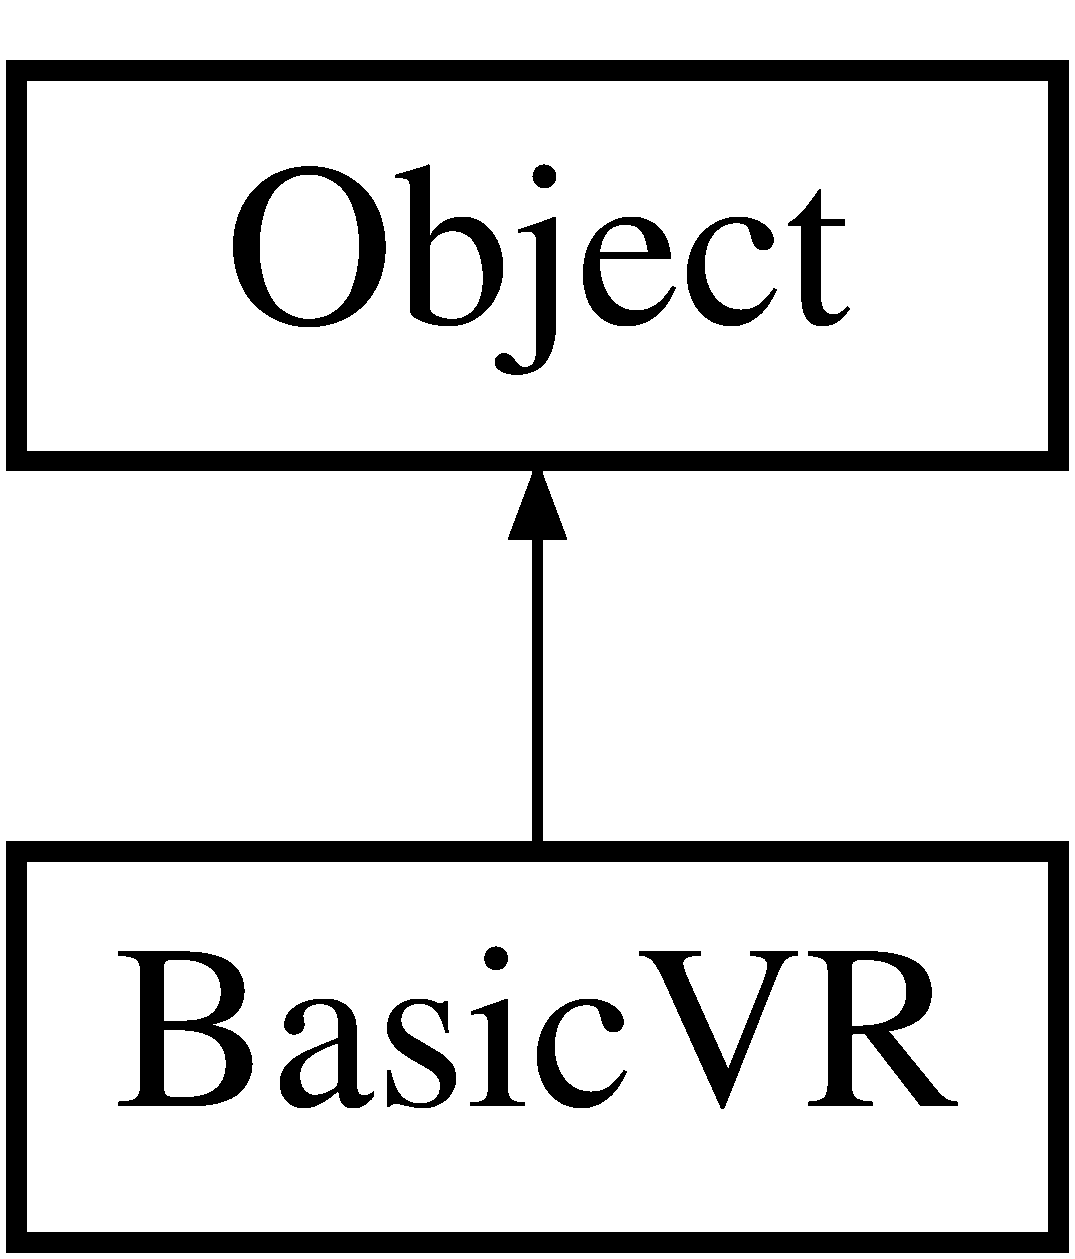
\includegraphics[height=2.000000cm]{class_basic_v_r}
\end{center}
\end{figure}
\subsection*{Public Member Functions}
\begin{DoxyCompactItemize}
\item 
virtual void \hyperlink{class_basic_v_r_a229f8e7af10029a22ed4738ba08eafd3}{Main\+Loop} ()=0
\item 
\hyperlink{class_basic_v_r_a7ee74cd5d4af3acc033d275c026e05d2}{Basic\+VR} (H\+I\+N\+S\+T\+A\+N\+CE h\+Inst, L\+P\+C\+W\+S\+TR window\+Title=L\char`\"{}Panoramic\+V\+R\textbackslash{}0\char`\"{})
\begin{DoxyCompactList}\small\item\em Constructor. \end{DoxyCompactList}\item 
bool \hyperlink{class_basic_v_r_a55ffc19ef7b92e30a3b173365a29a2ba}{Init} ()
\item 
virtual \hyperlink{class_basic_v_r_ada5417f4e5119c81dd8020c5cd1a0720}{$\sim$\+Basic\+VR} ()
\begin{DoxyCompactList}\small\item\em Destructor. \end{DoxyCompactList}\item 
void \hyperlink{class_basic_v_r_a3c5ef352017729bbd5646fa7a24367e2}{Action\+From\+Input} ()
\begin{DoxyCompactList}\small\item\em Functions. \end{DoxyCompactList}\item 
void \hyperlink{class_basic_v_r_aeff1e4ec95030046365b0804379890f7}{Distort\+And\+Present} (int num\+Layers\+To\+Render)
\item 
bool \hyperlink{class_basic_v_r_a155d1191d162ac1575ee6eb199ee7781}{Handle\+Messages} ()
\item 
void \hyperlink{class_basic_v_r_a0e7d89bc894e137c2bc67ae72ecba8ff}{Release\+Device} ()
\item 
int \hyperlink{class_basic_v_r_ab2068ad6695eabb935e83fa1dd4cdc8d}{Run} ()
\end{DoxyCompactItemize}
\subsection*{Protected Attributes}
\begin{DoxyCompactItemize}
\item 
H\+I\+N\+S\+T\+A\+N\+CE \hyperlink{class_basic_v_r_a5742130f7f3380da8e15a5f18b2b9f9b}{my\+H\+Instance}
\item 
L\+P\+C\+W\+S\+TR \hyperlink{class_basic_v_r_a3d17ef45cc13b39c7bd7e0106e6701db}{my\+Window\+Title}
\item 
ovr\+Hmd \hyperlink{class_basic_v_r_a23836eafb746bb2b92231beff9a9d76f}{my\+H\+MD}
\item 
ovr\+Hmd\+Desc \hyperlink{class_basic_v_r_aac00280b306310fd91944252dc422920}{my\+H\+M\+D\+Description}
\item 
ovr\+Result \hyperlink{class_basic_v_r_abf70fd52f6d3d9b3e471ce6b901b1a98}{my\+Current\+Result}
\item 
ovr\+Texture $\ast$ \hyperlink{class_basic_v_r_a07cc999ed9b14415166f909d0668b541}{my\+Mirror\+Texture}
\item 
\hyperlink{class_v_r_layer}{V\+R\+Layer} $\ast$ \hyperlink{class_basic_v_r_a2833a6f257610c214ed056c15a7f7785}{my\+V\+R\+Layers} \mbox{[}M\+A\+X\+\_\+\+L\+A\+Y\+E\+RS\mbox{]}
\item 
\hyperlink{class_camera}{Camera} $\ast$ \hyperlink{class_basic_v_r_a6c5320ef1fd4a951275da8d061bf71f8}{my\+Main\+Camera}
\item 
\hyperlink{class_scene}{Scene} $\ast$ \hyperlink{class_basic_v_r_a22a227877993e0f8cb1a1c8ed87070da}{my\+Room\+Scene}
\item 
Keyboard $\ast$ \hyperlink{class_basic_v_r_a2f9da8e8ccf48ce62e67a5e9e7f1be39}{my\+Keyboard}
\item 
Keyboard\+::\+Keyboard\+State\+Tracker $\ast$ \hyperlink{class_basic_v_r_acb6048b16b951dad8ba260453b455696}{my\+Keyboard\+State\+Tracker}
\item 
bool \hyperlink{class_basic_v_r_ac473465e66957471452478235fecfbe8}{my\+Is\+Initialized}
\item 
bool \hyperlink{class_basic_v_r_af0f6d4d8948900bac113d0eb3e3766ac}{my\+Is\+Windowed}
\item 
float \hyperlink{class_basic_v_r_ac6a774a1d2c2a6e49b70920a77363c83}{my\+Window\+Width\+Scale}
\item 
float \hyperlink{class_basic_v_r_a920b493bbb4217990d0c36dda41fa606}{my\+Window\+Height\+Scale}
\item 
float \hyperlink{class_basic_v_r_a0f45f5c5f10a425de415f40052380ce4}{my\+Mirror\+Width\+Scale}
\item 
float \hyperlink{class_basic_v_r_a0bdb21d619d8bf865c6852d62e6f73cb}{my\+Mirror\+Height\+Scale}
\item 
char $\ast$ \hyperlink{class_basic_v_r_a2d2fd1c9a0519b66eac327b5904d8122}{my\+Image\+File\+Path}
\item 
char $\ast$ \hyperlink{class_basic_v_r_a8b697e10768bada9a41bae38612f664f}{my\+Texture\+Tool\+Path}
\item 
char $\ast$ \hyperlink{class_basic_v_r_a3196ad5cd3083f927de0112c50252778}{my\+Texture\+Output\+Path}
\item 
char $\ast$ \hyperlink{class_basic_v_r_adc26337acc0de5285c226b5ef78b70d2}{my\+Config\+File\+Path}
\item 
char $\ast$ \hyperlink{class_basic_v_r_a74abf1122992a397a3412f4369d5a2e2}{my\+Vertex\+Shader\+Path}
\item 
char $\ast$ \hyperlink{class_basic_v_r_adf9127ec187e79b5e8b76f99daaa821a}{my\+Pixel\+Shader\+Path}
\end{DoxyCompactItemize}
\subsection*{Additional Inherited Members}


\subsection{Constructor \& Destructor Documentation}
\index{Basic\+VR@{Basic\+VR}!Basic\+VR@{Basic\+VR}}
\index{Basic\+VR@{Basic\+VR}!Basic\+VR@{Basic\+VR}}
\subsubsection[{\texorpdfstring{Basic\+V\+R(\+H\+I\+N\+S\+T\+A\+N\+C\+E h\+Inst, L\+P\+C\+W\+S\+T\+R window\+Title=L""Panoramic\+V\+R\textbackslash{}0"")}{BasicVR(HINSTANCE hInst, LPCWSTR windowTitle=L"PanoramicVR\textbackslash{}0")}}]{\setlength{\rightskip}{0pt plus 5cm}Basic\+V\+R\+::\+Basic\+VR (
\begin{DoxyParamCaption}
\item[{H\+I\+N\+S\+T\+A\+N\+CE}]{h\+Inst, }
\item[{L\+P\+C\+W\+S\+TR}]{window\+Title = {\ttfamily L\char`\"{}PanoramicVR\textbackslash{}0\char`\"{}}}
\end{DoxyParamCaption}
)}\hypertarget{class_basic_v_r_a7ee74cd5d4af3acc033d275c026e05d2}{}\label{class_basic_v_r_a7ee74cd5d4af3acc033d275c026e05d2}


Constructor. 

Constructor.

\begin{DoxyAuthor}{Author}
Katianie 
\end{DoxyAuthor}
\begin{DoxyDate}{Date}
7/4/2016
\end{DoxyDate}

\begin{DoxyParams}{Parameters}
{\em h\+Inst} & The instance. \\
\hline
{\em window\+Title} & The window title. \\
\hline
\end{DoxyParams}
\index{Basic\+VR@{Basic\+VR}!````~Basic\+VR@{$\sim$\+Basic\+VR}}
\index{````~Basic\+VR@{$\sim$\+Basic\+VR}!Basic\+VR@{Basic\+VR}}
\subsubsection[{\texorpdfstring{$\sim$\+Basic\+V\+R()}{~BasicVR()}}]{\setlength{\rightskip}{0pt plus 5cm}Basic\+V\+R\+::$\sim$\+Basic\+VR (
\begin{DoxyParamCaption}
{}
\end{DoxyParamCaption}
)\hspace{0.3cm}{\ttfamily [virtual]}}\hypertarget{class_basic_v_r_ada5417f4e5119c81dd8020c5cd1a0720}{}\label{class_basic_v_r_ada5417f4e5119c81dd8020c5cd1a0720}


Destructor. 

Destructor, Calls \hyperlink{class_basic_v_r_a0e7d89bc894e137c2bc67ae72ecba8ff}{Release\+Device()}.

\begin{DoxyAuthor}{Author}
Katianie 
\end{DoxyAuthor}
\begin{DoxyDate}{Date}
7/4/2016 
\end{DoxyDate}


\subsection{Member Function Documentation}
\index{Basic\+VR@{Basic\+VR}!Action\+From\+Input@{Action\+From\+Input}}
\index{Action\+From\+Input@{Action\+From\+Input}!Basic\+VR@{Basic\+VR}}
\subsubsection[{\texorpdfstring{Action\+From\+Input()}{ActionFromInput()}}]{\setlength{\rightskip}{0pt plus 5cm}void Basic\+V\+R\+::\+Action\+From\+Input (
\begin{DoxyParamCaption}
{}
\end{DoxyParamCaption}
)}\hypertarget{class_basic_v_r_a3c5ef352017729bbd5646fa7a24367e2}{}\label{class_basic_v_r_a3c5ef352017729bbd5646fa7a24367e2}


Functions. 

Listens for keyboard input and when Right or Left is pressed, the current scene is destroyed and then the next/previous scene is loaded.

\begin{DoxyAuthor}{Author}
Katianie 
\end{DoxyAuthor}
\begin{DoxyDate}{Date}
7/4/2016 
\end{DoxyDate}
\index{Basic\+VR@{Basic\+VR}!Distort\+And\+Present@{Distort\+And\+Present}}
\index{Distort\+And\+Present@{Distort\+And\+Present}!Basic\+VR@{Basic\+VR}}
\subsubsection[{\texorpdfstring{Distort\+And\+Present(int num\+Layers\+To\+Render)}{DistortAndPresent(int numLayersToRender)}}]{\setlength{\rightskip}{0pt plus 5cm}void Basic\+V\+R\+::\+Distort\+And\+Present (
\begin{DoxyParamCaption}
\item[{int}]{num\+Layers\+To\+Render}
\end{DoxyParamCaption}
)}\hypertarget{class_basic_v_r_aeff1e4ec95030046365b0804379890f7}{}\label{class_basic_v_r_aeff1e4ec95030046365b0804379890f7}
Distort and present.

\begin{DoxyAuthor}{Author}
Katianie 
\end{DoxyAuthor}
\begin{DoxyDate}{Date}
7/4/2016
\end{DoxyDate}

\begin{DoxyParams}{Parameters}
{\em num\+Layers\+To\+Render} & Number of layers to render. \\
\hline
\end{DoxyParams}
\index{Basic\+VR@{Basic\+VR}!Handle\+Messages@{Handle\+Messages}}
\index{Handle\+Messages@{Handle\+Messages}!Basic\+VR@{Basic\+VR}}
\subsubsection[{\texorpdfstring{Handle\+Messages()}{HandleMessages()}}]{\setlength{\rightskip}{0pt plus 5cm}bool Basic\+V\+R\+::\+Handle\+Messages (
\begin{DoxyParamCaption}
{}
\end{DoxyParamCaption}
)}\hypertarget{class_basic_v_r_a155d1191d162ac1575ee6eb199ee7781}{}\label{class_basic_v_r_a155d1191d162ac1575ee6eb199ee7781}
Handles windows messages.

\begin{DoxyAuthor}{Author}
Katianie 
\end{DoxyAuthor}
\begin{DoxyDate}{Date}
7/4/2016
\end{DoxyDate}
\begin{DoxyReturn}{Returns}
true if it succeeds, false if it fails. 
\end{DoxyReturn}
\index{Basic\+VR@{Basic\+VR}!Init@{Init}}
\index{Init@{Init}!Basic\+VR@{Basic\+VR}}
\subsubsection[{\texorpdfstring{Init()}{Init()}}]{\setlength{\rightskip}{0pt plus 5cm}bool Basic\+V\+R\+::\+Init (
\begin{DoxyParamCaption}
{}
\end{DoxyParamCaption}
)}\hypertarget{class_basic_v_r_a55ffc19ef7b92e30a3b173365a29a2ba}{}\label{class_basic_v_r_a55ffc19ef7b92e30a3b173365a29a2ba}
Initializes the \hyperlink{class_scene}{Scene}, \hyperlink{class_camera}{Camera}, Keyboard, and the Mirror window.

\begin{DoxyAuthor}{Author}
Katianie 
\end{DoxyAuthor}
\begin{DoxyDate}{Date}
7/4/2016
\end{DoxyDate}
\begin{DoxyReturn}{Returns}
true if initialization was successful, false if it fails. 
\end{DoxyReturn}
\index{Basic\+VR@{Basic\+VR}!Main\+Loop@{Main\+Loop}}
\index{Main\+Loop@{Main\+Loop}!Basic\+VR@{Basic\+VR}}
\subsubsection[{\texorpdfstring{Main\+Loop()=0}{MainLoop()=0}}]{\setlength{\rightskip}{0pt plus 5cm}virtual void Basic\+V\+R\+::\+Main\+Loop (
\begin{DoxyParamCaption}
{}
\end{DoxyParamCaption}
)\hspace{0.3cm}{\ttfamily [pure virtual]}}\hypertarget{class_basic_v_r_a229f8e7af10029a22ed4738ba08eafd3}{}\label{class_basic_v_r_a229f8e7af10029a22ed4738ba08eafd3}
\index{Basic\+VR@{Basic\+VR}!Release\+Device@{Release\+Device}}
\index{Release\+Device@{Release\+Device}!Basic\+VR@{Basic\+VR}}
\subsubsection[{\texorpdfstring{Release\+Device()}{ReleaseDevice()}}]{\setlength{\rightskip}{0pt plus 5cm}void Basic\+V\+R\+::\+Release\+Device (
\begin{DoxyParamCaption}
{}
\end{DoxyParamCaption}
)}\hypertarget{class_basic_v_r_a0e7d89bc894e137c2bc67ae72ecba8ff}{}\label{class_basic_v_r_a0e7d89bc894e137c2bc67ae72ecba8ff}
Destroy and delete all objects and release the device. Also shuts down O\+VR and exits the program with exit(0).

\begin{DoxyAuthor}{Author}
Katianie 
\end{DoxyAuthor}
\begin{DoxyDate}{Date}
7/4/2016 
\end{DoxyDate}
\index{Basic\+VR@{Basic\+VR}!Run@{Run}}
\index{Run@{Run}!Basic\+VR@{Basic\+VR}}
\subsubsection[{\texorpdfstring{Run()}{Run()}}]{\setlength{\rightskip}{0pt plus 5cm}int Basic\+V\+R\+::\+Run (
\begin{DoxyParamCaption}
{}
\end{DoxyParamCaption}
)}\hypertarget{class_basic_v_r_ab2068ad6695eabb935e83fa1dd4cdc8d}{}\label{class_basic_v_r_ab2068ad6695eabb935e83fa1dd4cdc8d}
The main loop for the application. This is triggered in the child classes (i.\+e. main.\+cpp).

\begin{DoxyAuthor}{Author}
Katianie 
\end{DoxyAuthor}
\begin{DoxyDate}{Date}
7/4/2016
\end{DoxyDate}
\begin{DoxyReturn}{Returns}
0 on success. 
\end{DoxyReturn}


\subsection{Member Data Documentation}
\index{Basic\+VR@{Basic\+VR}!my\+Config\+File\+Path@{my\+Config\+File\+Path}}
\index{my\+Config\+File\+Path@{my\+Config\+File\+Path}!Basic\+VR@{Basic\+VR}}
\subsubsection[{\texorpdfstring{my\+Config\+File\+Path}{myConfigFilePath}}]{\setlength{\rightskip}{0pt plus 5cm}char$\ast$ Basic\+V\+R\+::my\+Config\+File\+Path\hspace{0.3cm}{\ttfamily [protected]}}\hypertarget{class_basic_v_r_adc26337acc0de5285c226b5ef78b70d2}{}\label{class_basic_v_r_adc26337acc0de5285c226b5ef78b70d2}
\index{Basic\+VR@{Basic\+VR}!my\+Current\+Result@{my\+Current\+Result}}
\index{my\+Current\+Result@{my\+Current\+Result}!Basic\+VR@{Basic\+VR}}
\subsubsection[{\texorpdfstring{my\+Current\+Result}{myCurrentResult}}]{\setlength{\rightskip}{0pt plus 5cm}ovr\+Result Basic\+V\+R\+::my\+Current\+Result\hspace{0.3cm}{\ttfamily [protected]}}\hypertarget{class_basic_v_r_abf70fd52f6d3d9b3e471ce6b901b1a98}{}\label{class_basic_v_r_abf70fd52f6d3d9b3e471ce6b901b1a98}
\index{Basic\+VR@{Basic\+VR}!my\+H\+Instance@{my\+H\+Instance}}
\index{my\+H\+Instance@{my\+H\+Instance}!Basic\+VR@{Basic\+VR}}
\subsubsection[{\texorpdfstring{my\+H\+Instance}{myHInstance}}]{\setlength{\rightskip}{0pt plus 5cm}H\+I\+N\+S\+T\+A\+N\+CE Basic\+V\+R\+::my\+H\+Instance\hspace{0.3cm}{\ttfamily [protected]}}\hypertarget{class_basic_v_r_a5742130f7f3380da8e15a5f18b2b9f9b}{}\label{class_basic_v_r_a5742130f7f3380da8e15a5f18b2b9f9b}
\index{Basic\+VR@{Basic\+VR}!my\+H\+MD@{my\+H\+MD}}
\index{my\+H\+MD@{my\+H\+MD}!Basic\+VR@{Basic\+VR}}
\subsubsection[{\texorpdfstring{my\+H\+MD}{myHMD}}]{\setlength{\rightskip}{0pt plus 5cm}ovr\+Hmd Basic\+V\+R\+::my\+H\+MD\hspace{0.3cm}{\ttfamily [protected]}}\hypertarget{class_basic_v_r_a23836eafb746bb2b92231beff9a9d76f}{}\label{class_basic_v_r_a23836eafb746bb2b92231beff9a9d76f}
\index{Basic\+VR@{Basic\+VR}!my\+H\+M\+D\+Description@{my\+H\+M\+D\+Description}}
\index{my\+H\+M\+D\+Description@{my\+H\+M\+D\+Description}!Basic\+VR@{Basic\+VR}}
\subsubsection[{\texorpdfstring{my\+H\+M\+D\+Description}{myHMDDescription}}]{\setlength{\rightskip}{0pt plus 5cm}ovr\+Hmd\+Desc Basic\+V\+R\+::my\+H\+M\+D\+Description\hspace{0.3cm}{\ttfamily [protected]}}\hypertarget{class_basic_v_r_aac00280b306310fd91944252dc422920}{}\label{class_basic_v_r_aac00280b306310fd91944252dc422920}
\index{Basic\+VR@{Basic\+VR}!my\+Image\+File\+Path@{my\+Image\+File\+Path}}
\index{my\+Image\+File\+Path@{my\+Image\+File\+Path}!Basic\+VR@{Basic\+VR}}
\subsubsection[{\texorpdfstring{my\+Image\+File\+Path}{myImageFilePath}}]{\setlength{\rightskip}{0pt plus 5cm}char$\ast$ Basic\+V\+R\+::my\+Image\+File\+Path\hspace{0.3cm}{\ttfamily [protected]}}\hypertarget{class_basic_v_r_a2d2fd1c9a0519b66eac327b5904d8122}{}\label{class_basic_v_r_a2d2fd1c9a0519b66eac327b5904d8122}
\index{Basic\+VR@{Basic\+VR}!my\+Is\+Initialized@{my\+Is\+Initialized}}
\index{my\+Is\+Initialized@{my\+Is\+Initialized}!Basic\+VR@{Basic\+VR}}
\subsubsection[{\texorpdfstring{my\+Is\+Initialized}{myIsInitialized}}]{\setlength{\rightskip}{0pt plus 5cm}bool Basic\+V\+R\+::my\+Is\+Initialized\hspace{0.3cm}{\ttfamily [protected]}}\hypertarget{class_basic_v_r_ac473465e66957471452478235fecfbe8}{}\label{class_basic_v_r_ac473465e66957471452478235fecfbe8}
\index{Basic\+VR@{Basic\+VR}!my\+Is\+Windowed@{my\+Is\+Windowed}}
\index{my\+Is\+Windowed@{my\+Is\+Windowed}!Basic\+VR@{Basic\+VR}}
\subsubsection[{\texorpdfstring{my\+Is\+Windowed}{myIsWindowed}}]{\setlength{\rightskip}{0pt plus 5cm}bool Basic\+V\+R\+::my\+Is\+Windowed\hspace{0.3cm}{\ttfamily [protected]}}\hypertarget{class_basic_v_r_af0f6d4d8948900bac113d0eb3e3766ac}{}\label{class_basic_v_r_af0f6d4d8948900bac113d0eb3e3766ac}
\index{Basic\+VR@{Basic\+VR}!my\+Keyboard@{my\+Keyboard}}
\index{my\+Keyboard@{my\+Keyboard}!Basic\+VR@{Basic\+VR}}
\subsubsection[{\texorpdfstring{my\+Keyboard}{myKeyboard}}]{\setlength{\rightskip}{0pt plus 5cm}Keyboard$\ast$ Basic\+V\+R\+::my\+Keyboard\hspace{0.3cm}{\ttfamily [protected]}}\hypertarget{class_basic_v_r_a2f9da8e8ccf48ce62e67a5e9e7f1be39}{}\label{class_basic_v_r_a2f9da8e8ccf48ce62e67a5e9e7f1be39}
\index{Basic\+VR@{Basic\+VR}!my\+Keyboard\+State\+Tracker@{my\+Keyboard\+State\+Tracker}}
\index{my\+Keyboard\+State\+Tracker@{my\+Keyboard\+State\+Tracker}!Basic\+VR@{Basic\+VR}}
\subsubsection[{\texorpdfstring{my\+Keyboard\+State\+Tracker}{myKeyboardStateTracker}}]{\setlength{\rightskip}{0pt plus 5cm}Keyboard\+::\+Keyboard\+State\+Tracker$\ast$ Basic\+V\+R\+::my\+Keyboard\+State\+Tracker\hspace{0.3cm}{\ttfamily [protected]}}\hypertarget{class_basic_v_r_acb6048b16b951dad8ba260453b455696}{}\label{class_basic_v_r_acb6048b16b951dad8ba260453b455696}
\index{Basic\+VR@{Basic\+VR}!my\+Main\+Camera@{my\+Main\+Camera}}
\index{my\+Main\+Camera@{my\+Main\+Camera}!Basic\+VR@{Basic\+VR}}
\subsubsection[{\texorpdfstring{my\+Main\+Camera}{myMainCamera}}]{\setlength{\rightskip}{0pt plus 5cm}{\bf Camera}$\ast$ Basic\+V\+R\+::my\+Main\+Camera\hspace{0.3cm}{\ttfamily [protected]}}\hypertarget{class_basic_v_r_a6c5320ef1fd4a951275da8d061bf71f8}{}\label{class_basic_v_r_a6c5320ef1fd4a951275da8d061bf71f8}
\index{Basic\+VR@{Basic\+VR}!my\+Mirror\+Height\+Scale@{my\+Mirror\+Height\+Scale}}
\index{my\+Mirror\+Height\+Scale@{my\+Mirror\+Height\+Scale}!Basic\+VR@{Basic\+VR}}
\subsubsection[{\texorpdfstring{my\+Mirror\+Height\+Scale}{myMirrorHeightScale}}]{\setlength{\rightskip}{0pt plus 5cm}float Basic\+V\+R\+::my\+Mirror\+Height\+Scale\hspace{0.3cm}{\ttfamily [protected]}}\hypertarget{class_basic_v_r_a0bdb21d619d8bf865c6852d62e6f73cb}{}\label{class_basic_v_r_a0bdb21d619d8bf865c6852d62e6f73cb}
\index{Basic\+VR@{Basic\+VR}!my\+Mirror\+Texture@{my\+Mirror\+Texture}}
\index{my\+Mirror\+Texture@{my\+Mirror\+Texture}!Basic\+VR@{Basic\+VR}}
\subsubsection[{\texorpdfstring{my\+Mirror\+Texture}{myMirrorTexture}}]{\setlength{\rightskip}{0pt plus 5cm}ovr\+Texture$\ast$ Basic\+V\+R\+::my\+Mirror\+Texture\hspace{0.3cm}{\ttfamily [protected]}}\hypertarget{class_basic_v_r_a07cc999ed9b14415166f909d0668b541}{}\label{class_basic_v_r_a07cc999ed9b14415166f909d0668b541}
\index{Basic\+VR@{Basic\+VR}!my\+Mirror\+Width\+Scale@{my\+Mirror\+Width\+Scale}}
\index{my\+Mirror\+Width\+Scale@{my\+Mirror\+Width\+Scale}!Basic\+VR@{Basic\+VR}}
\subsubsection[{\texorpdfstring{my\+Mirror\+Width\+Scale}{myMirrorWidthScale}}]{\setlength{\rightskip}{0pt plus 5cm}float Basic\+V\+R\+::my\+Mirror\+Width\+Scale\hspace{0.3cm}{\ttfamily [protected]}}\hypertarget{class_basic_v_r_a0f45f5c5f10a425de415f40052380ce4}{}\label{class_basic_v_r_a0f45f5c5f10a425de415f40052380ce4}
\index{Basic\+VR@{Basic\+VR}!my\+Pixel\+Shader\+Path@{my\+Pixel\+Shader\+Path}}
\index{my\+Pixel\+Shader\+Path@{my\+Pixel\+Shader\+Path}!Basic\+VR@{Basic\+VR}}
\subsubsection[{\texorpdfstring{my\+Pixel\+Shader\+Path}{myPixelShaderPath}}]{\setlength{\rightskip}{0pt plus 5cm}char$\ast$ Basic\+V\+R\+::my\+Pixel\+Shader\+Path\hspace{0.3cm}{\ttfamily [protected]}}\hypertarget{class_basic_v_r_adf9127ec187e79b5e8b76f99daaa821a}{}\label{class_basic_v_r_adf9127ec187e79b5e8b76f99daaa821a}
\index{Basic\+VR@{Basic\+VR}!my\+Room\+Scene@{my\+Room\+Scene}}
\index{my\+Room\+Scene@{my\+Room\+Scene}!Basic\+VR@{Basic\+VR}}
\subsubsection[{\texorpdfstring{my\+Room\+Scene}{myRoomScene}}]{\setlength{\rightskip}{0pt plus 5cm}{\bf Scene}$\ast$ Basic\+V\+R\+::my\+Room\+Scene\hspace{0.3cm}{\ttfamily [protected]}}\hypertarget{class_basic_v_r_a22a227877993e0f8cb1a1c8ed87070da}{}\label{class_basic_v_r_a22a227877993e0f8cb1a1c8ed87070da}
\index{Basic\+VR@{Basic\+VR}!my\+Texture\+Output\+Path@{my\+Texture\+Output\+Path}}
\index{my\+Texture\+Output\+Path@{my\+Texture\+Output\+Path}!Basic\+VR@{Basic\+VR}}
\subsubsection[{\texorpdfstring{my\+Texture\+Output\+Path}{myTextureOutputPath}}]{\setlength{\rightskip}{0pt plus 5cm}char$\ast$ Basic\+V\+R\+::my\+Texture\+Output\+Path\hspace{0.3cm}{\ttfamily [protected]}}\hypertarget{class_basic_v_r_a3196ad5cd3083f927de0112c50252778}{}\label{class_basic_v_r_a3196ad5cd3083f927de0112c50252778}
\index{Basic\+VR@{Basic\+VR}!my\+Texture\+Tool\+Path@{my\+Texture\+Tool\+Path}}
\index{my\+Texture\+Tool\+Path@{my\+Texture\+Tool\+Path}!Basic\+VR@{Basic\+VR}}
\subsubsection[{\texorpdfstring{my\+Texture\+Tool\+Path}{myTextureToolPath}}]{\setlength{\rightskip}{0pt plus 5cm}char$\ast$ Basic\+V\+R\+::my\+Texture\+Tool\+Path\hspace{0.3cm}{\ttfamily [protected]}}\hypertarget{class_basic_v_r_a8b697e10768bada9a41bae38612f664f}{}\label{class_basic_v_r_a8b697e10768bada9a41bae38612f664f}
\index{Basic\+VR@{Basic\+VR}!my\+Vertex\+Shader\+Path@{my\+Vertex\+Shader\+Path}}
\index{my\+Vertex\+Shader\+Path@{my\+Vertex\+Shader\+Path}!Basic\+VR@{Basic\+VR}}
\subsubsection[{\texorpdfstring{my\+Vertex\+Shader\+Path}{myVertexShaderPath}}]{\setlength{\rightskip}{0pt plus 5cm}char$\ast$ Basic\+V\+R\+::my\+Vertex\+Shader\+Path\hspace{0.3cm}{\ttfamily [protected]}}\hypertarget{class_basic_v_r_a74abf1122992a397a3412f4369d5a2e2}{}\label{class_basic_v_r_a74abf1122992a397a3412f4369d5a2e2}
\index{Basic\+VR@{Basic\+VR}!my\+V\+R\+Layers@{my\+V\+R\+Layers}}
\index{my\+V\+R\+Layers@{my\+V\+R\+Layers}!Basic\+VR@{Basic\+VR}}
\subsubsection[{\texorpdfstring{my\+V\+R\+Layers}{myVRLayers}}]{\setlength{\rightskip}{0pt plus 5cm}{\bf V\+R\+Layer}$\ast$ Basic\+V\+R\+::my\+V\+R\+Layers\mbox{[}M\+A\+X\+\_\+\+L\+A\+Y\+E\+RS\mbox{]}\hspace{0.3cm}{\ttfamily [protected]}}\hypertarget{class_basic_v_r_a2833a6f257610c214ed056c15a7f7785}{}\label{class_basic_v_r_a2833a6f257610c214ed056c15a7f7785}
\index{Basic\+VR@{Basic\+VR}!my\+Window\+Height\+Scale@{my\+Window\+Height\+Scale}}
\index{my\+Window\+Height\+Scale@{my\+Window\+Height\+Scale}!Basic\+VR@{Basic\+VR}}
\subsubsection[{\texorpdfstring{my\+Window\+Height\+Scale}{myWindowHeightScale}}]{\setlength{\rightskip}{0pt plus 5cm}float Basic\+V\+R\+::my\+Window\+Height\+Scale\hspace{0.3cm}{\ttfamily [protected]}}\hypertarget{class_basic_v_r_a920b493bbb4217990d0c36dda41fa606}{}\label{class_basic_v_r_a920b493bbb4217990d0c36dda41fa606}
\index{Basic\+VR@{Basic\+VR}!my\+Window\+Title@{my\+Window\+Title}}
\index{my\+Window\+Title@{my\+Window\+Title}!Basic\+VR@{Basic\+VR}}
\subsubsection[{\texorpdfstring{my\+Window\+Title}{myWindowTitle}}]{\setlength{\rightskip}{0pt plus 5cm}L\+P\+C\+W\+S\+TR Basic\+V\+R\+::my\+Window\+Title\hspace{0.3cm}{\ttfamily [protected]}}\hypertarget{class_basic_v_r_a3d17ef45cc13b39c7bd7e0106e6701db}{}\label{class_basic_v_r_a3d17ef45cc13b39c7bd7e0106e6701db}
\index{Basic\+VR@{Basic\+VR}!my\+Window\+Width\+Scale@{my\+Window\+Width\+Scale}}
\index{my\+Window\+Width\+Scale@{my\+Window\+Width\+Scale}!Basic\+VR@{Basic\+VR}}
\subsubsection[{\texorpdfstring{my\+Window\+Width\+Scale}{myWindowWidthScale}}]{\setlength{\rightskip}{0pt plus 5cm}float Basic\+V\+R\+::my\+Window\+Width\+Scale\hspace{0.3cm}{\ttfamily [protected]}}\hypertarget{class_basic_v_r_ac6a774a1d2c2a6e49b70920a77363c83}{}\label{class_basic_v_r_ac6a774a1d2c2a6e49b70920a77363c83}


The documentation for this class was generated from the following files\+:\begin{DoxyCompactItemize}
\item 
Samples/\+Oculus\+Room\+Tiny\+\_\+\+Advanced/\+Common/\+Headers/\hyperlink{_basic_v_r_8h}{Basic\+V\+R.\+h}\item 
Samples/\+Oculus\+Room\+Tiny\+\_\+\+Advanced/\+Common/\+Implementations/\hyperlink{_basic_v_r_8cpp}{Basic\+V\+R.\+cpp}\end{DoxyCompactItemize}

\hypertarget{class_camera}{}\section{Camera Class Reference}
\label{class_camera}\index{Camera@{Camera}}


{\ttfamily \#include $<$Camera.\+h$>$}

Inheritance diagram for Camera\+:\begin{figure}[H]
\begin{center}
\leavevmode
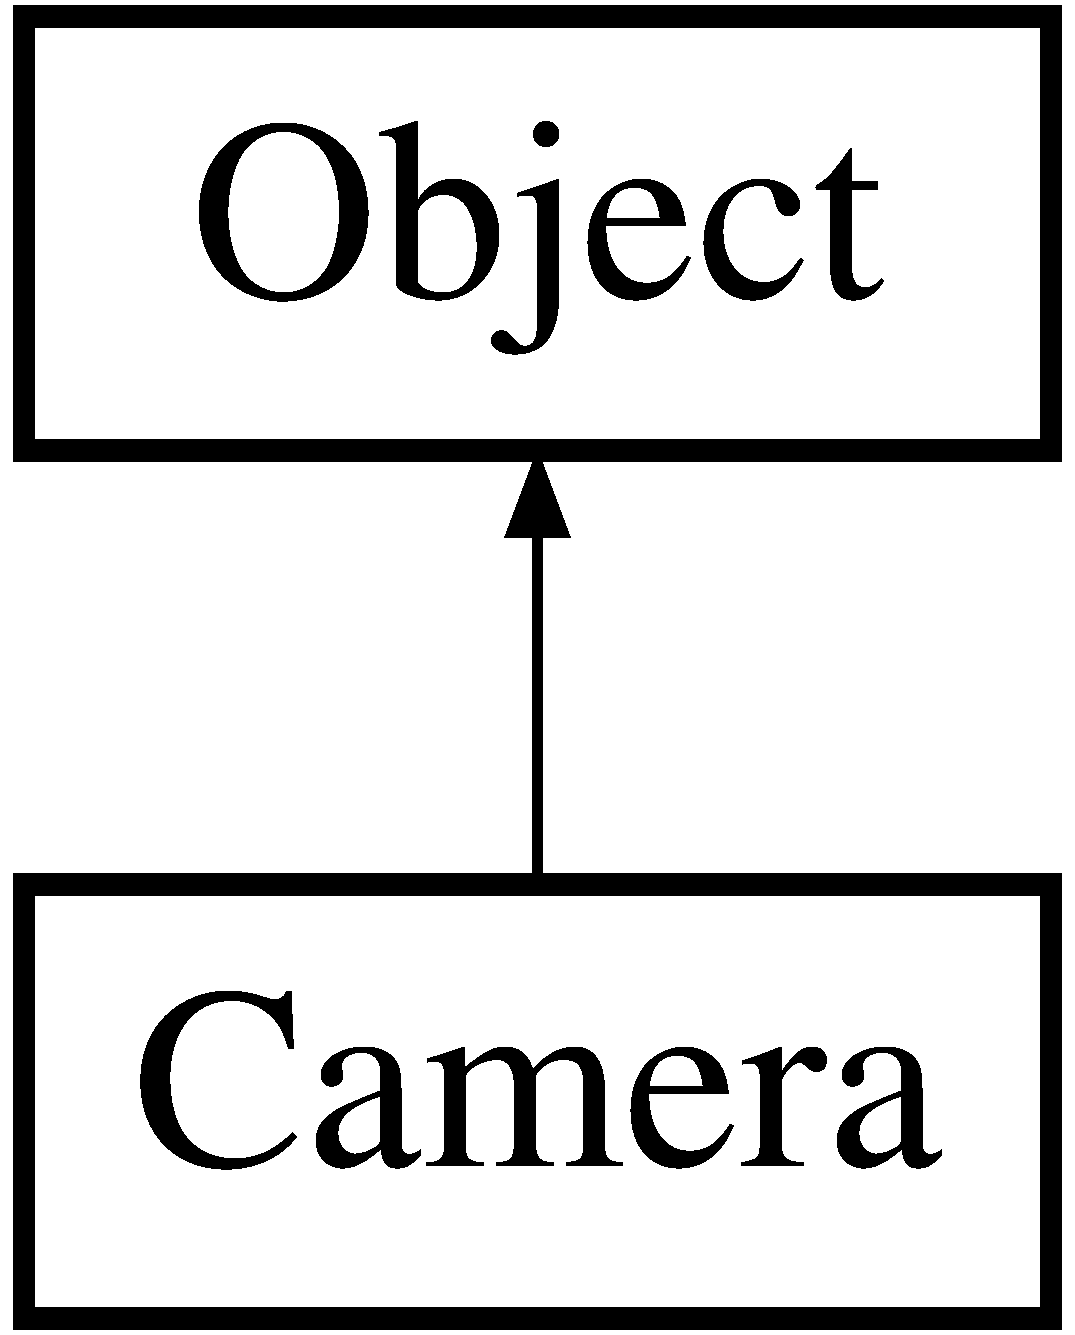
\includegraphics[height=2.000000cm]{class_camera}
\end{center}
\end{figure}
\subsection*{Public Member Functions}
\begin{DoxyCompactItemize}
\item 
\hyperlink{class_camera_a01f94c3543f56ede7af49dc778f19331}{Camera} ()
\begin{DoxyCompactList}\small\item\em Constructors. \end{DoxyCompactList}\item 
\hyperlink{class_camera_a029be94b2307a3ffeb0de58769dc6d6e}{Camera} (X\+M\+V\+E\+C\+T\+OR $\ast$position, X\+M\+V\+E\+C\+T\+OR $\ast$rotation)
\item 
void \hyperlink{class_camera_a2cb449dfd69fc002ab6117d71c6af1ff}{Init} (X\+M\+V\+E\+C\+T\+OR position, X\+M\+V\+E\+C\+T\+OR rotation)
\item 
virtual \hyperlink{class_camera_ad1897942d0ccf91052386388a497349f}{$\sim$\+Camera} ()
\begin{DoxyCompactList}\small\item\em Destructor. \end{DoxyCompactList}\item 
X\+M\+V\+E\+C\+T\+OR \hyperlink{class_camera_a0ba4b24f3f39dedb32715dc787d1a75d}{Get\+Position} ()
\begin{DoxyCompactList}\small\item\em Getters. \end{DoxyCompactList}\item 
X\+M\+V\+E\+C\+T\+OR \hyperlink{class_camera_a374cad6c4aef593974bc96d5186dbcb2}{Get\+Rotation} ()
\item 
X\+M\+M\+A\+T\+R\+IX \hyperlink{class_camera_a2e6a80af72c230fafd8f5ec9f32db15b}{Get\+View\+Matrix} ()
\item 
void \hyperlink{class_camera_a6cdb52b1f4b0ebc7b2f581a02a761e10}{Set\+Position} (X\+M\+V\+E\+C\+T\+OR pos)
\begin{DoxyCompactList}\small\item\em Setters. \end{DoxyCompactList}\item 
void \hyperlink{class_camera_a66bf632272852abc17b5dc15cceb3591}{Set\+Rotation} (X\+M\+V\+E\+C\+T\+OR rot)
\end{DoxyCompactItemize}
\subsection*{Protected Attributes}
\begin{DoxyCompactItemize}
\item 
X\+M\+V\+E\+C\+T\+OR \hyperlink{class_camera_ae90a13af9d2b2f18b19e430a3b301ae9}{my\+Position}
\item 
X\+M\+V\+E\+C\+T\+OR \hyperlink{class_camera_a922f81f1d51693f48310a49d94c9a66e}{my\+Rotation}
\end{DoxyCompactItemize}
\subsection*{Additional Inherited Members}


\subsection{Constructor \& Destructor Documentation}
\index{Camera@{Camera}!Camera@{Camera}}
\index{Camera@{Camera}!Camera@{Camera}}
\subsubsection[{\texorpdfstring{Camera()}{Camera()}}]{\setlength{\rightskip}{0pt plus 5cm}Camera\+::\+Camera (
\begin{DoxyParamCaption}
{}
\end{DoxyParamCaption}
)}\hypertarget{class_camera_a01f94c3543f56ede7af49dc778f19331}{}\label{class_camera_a01f94c3543f56ede7af49dc778f19331}


Constructors. 

Default Constructor

\begin{DoxyAuthor}{Author}
Katianie 
\end{DoxyAuthor}
\begin{DoxyDate}{Date}
7/4/2016 
\end{DoxyDate}
\index{Camera@{Camera}!Camera@{Camera}}
\index{Camera@{Camera}!Camera@{Camera}}
\subsubsection[{\texorpdfstring{Camera(\+X\+M\+V\+E\+C\+T\+O\+R $\ast$position, X\+M\+V\+E\+C\+T\+O\+R $\ast$rotation)}{Camera(XMVECTOR *position, XMVECTOR *rotation)}}]{\setlength{\rightskip}{0pt plus 5cm}Camera\+::\+Camera (
\begin{DoxyParamCaption}
\item[{X\+M\+V\+E\+C\+T\+OR $\ast$}]{position, }
\item[{X\+M\+V\+E\+C\+T\+OR $\ast$}]{rotation}
\end{DoxyParamCaption}
)}\hypertarget{class_camera_a029be94b2307a3ffeb0de58769dc6d6e}{}\label{class_camera_a029be94b2307a3ffeb0de58769dc6d6e}
Parameterized Constructor.

\begin{DoxyAuthor}{Author}
Katianie 
\end{DoxyAuthor}
\begin{DoxyDate}{Date}
7/4/2016
\end{DoxyDate}

\begin{DoxyParams}[1]{Parameters}
\mbox{\tt in}  & {\em position} & If non-\/null, the position. \\
\hline
\mbox{\tt in}  & {\em rotation} & If non-\/null, the rotation. \\
\hline
\end{DoxyParams}
\index{Camera@{Camera}!````~Camera@{$\sim$\+Camera}}
\index{````~Camera@{$\sim$\+Camera}!Camera@{Camera}}
\subsubsection[{\texorpdfstring{$\sim$\+Camera()}{~Camera()}}]{\setlength{\rightskip}{0pt plus 5cm}Camera\+::$\sim$\+Camera (
\begin{DoxyParamCaption}
{}
\end{DoxyParamCaption}
)\hspace{0.3cm}{\ttfamily [virtual]}}\hypertarget{class_camera_ad1897942d0ccf91052386388a497349f}{}\label{class_camera_ad1897942d0ccf91052386388a497349f}


Destructor. 

Destructor.

\begin{DoxyAuthor}{Author}
Katianie 
\end{DoxyAuthor}
\begin{DoxyDate}{Date}
7/4/2016 
\end{DoxyDate}


\subsection{Member Function Documentation}
\index{Camera@{Camera}!Get\+Position@{Get\+Position}}
\index{Get\+Position@{Get\+Position}!Camera@{Camera}}
\subsubsection[{\texorpdfstring{Get\+Position()}{GetPosition()}}]{\setlength{\rightskip}{0pt plus 5cm}X\+M\+V\+E\+C\+T\+OR Camera\+::\+Get\+Position (
\begin{DoxyParamCaption}
{}
\end{DoxyParamCaption}
)}\hypertarget{class_camera_a0ba4b24f3f39dedb32715dc787d1a75d}{}\label{class_camera_a0ba4b24f3f39dedb32715dc787d1a75d}


Getters. 

Gets the X,Y,Z Position of the \hyperlink{class_camera}{Camera}.

\begin{DoxyAuthor}{Author}
Katianie 
\end{DoxyAuthor}
\begin{DoxyDate}{Date}
7/4/2016
\end{DoxyDate}
\begin{DoxyReturn}{Returns}
The X,Y,Z Position of the \hyperlink{class_camera}{Camera}. 
\end{DoxyReturn}
\index{Camera@{Camera}!Get\+Rotation@{Get\+Rotation}}
\index{Get\+Rotation@{Get\+Rotation}!Camera@{Camera}}
\subsubsection[{\texorpdfstring{Get\+Rotation()}{GetRotation()}}]{\setlength{\rightskip}{0pt plus 5cm}X\+M\+V\+E\+C\+T\+OR Camera\+::\+Get\+Rotation (
\begin{DoxyParamCaption}
{}
\end{DoxyParamCaption}
)}\hypertarget{class_camera_a374cad6c4aef593974bc96d5186dbcb2}{}\label{class_camera_a374cad6c4aef593974bc96d5186dbcb2}
Gets the rotation vector of the camera.

\begin{DoxyAuthor}{Author}
Katianie 
\end{DoxyAuthor}
\begin{DoxyDate}{Date}
7/4/2016
\end{DoxyDate}
\begin{DoxyReturn}{Returns}
The rotation vector of the camera. 
\end{DoxyReturn}
\index{Camera@{Camera}!Get\+View\+Matrix@{Get\+View\+Matrix}}
\index{Get\+View\+Matrix@{Get\+View\+Matrix}!Camera@{Camera}}
\subsubsection[{\texorpdfstring{Get\+View\+Matrix()}{GetViewMatrix()}}]{\setlength{\rightskip}{0pt plus 5cm}X\+M\+M\+A\+T\+R\+IX Camera\+::\+Get\+View\+Matrix (
\begin{DoxyParamCaption}
{}
\end{DoxyParamCaption}
)}\hypertarget{class_camera_a2e6a80af72c230fafd8f5ec9f32db15b}{}\label{class_camera_a2e6a80af72c230fafd8f5ec9f32db15b}
Gets view matrix.

\begin{DoxyAuthor}{Author}
Katianie 
\end{DoxyAuthor}
\begin{DoxyDate}{Date}
7/4/2016
\end{DoxyDate}
\begin{DoxyReturn}{Returns}
The view matrix. 
\end{DoxyReturn}
\index{Camera@{Camera}!Init@{Init}}
\index{Init@{Init}!Camera@{Camera}}
\subsubsection[{\texorpdfstring{Init(\+X\+M\+V\+E\+C\+T\+O\+R position, X\+M\+V\+E\+C\+T\+O\+R rotation)}{Init(XMVECTOR position, XMVECTOR rotation)}}]{\setlength{\rightskip}{0pt plus 5cm}void Camera\+::\+Init (
\begin{DoxyParamCaption}
\item[{X\+M\+V\+E\+C\+T\+OR}]{position, }
\item[{X\+M\+V\+E\+C\+T\+OR}]{rotation}
\end{DoxyParamCaption}
)}\hypertarget{class_camera_a2cb449dfd69fc002ab6117d71c6af1ff}{}\label{class_camera_a2cb449dfd69fc002ab6117d71c6af1ff}
Initialized the instance variables of the \hyperlink{class_camera}{Camera}.

\begin{DoxyAuthor}{Author}
Katianie 
\end{DoxyAuthor}
\begin{DoxyDate}{Date}
7/4/2016
\end{DoxyDate}

\begin{DoxyParams}{Parameters}
{\em position} & The position. \\
\hline
{\em rotation} & The rotation. \\
\hline
\end{DoxyParams}
\index{Camera@{Camera}!Set\+Position@{Set\+Position}}
\index{Set\+Position@{Set\+Position}!Camera@{Camera}}
\subsubsection[{\texorpdfstring{Set\+Position(\+X\+M\+V\+E\+C\+T\+O\+R pos)}{SetPosition(XMVECTOR pos)}}]{\setlength{\rightskip}{0pt plus 5cm}void Camera\+::\+Set\+Position (
\begin{DoxyParamCaption}
\item[{X\+M\+V\+E\+C\+T\+OR}]{pos}
\end{DoxyParamCaption}
)}\hypertarget{class_camera_a6cdb52b1f4b0ebc7b2f581a02a761e10}{}\label{class_camera_a6cdb52b1f4b0ebc7b2f581a02a761e10}


Setters. 

Sets the X,Y,Z Position of the \hyperlink{class_camera}{Camera}.

\begin{DoxyAuthor}{Author}
Katianie 
\end{DoxyAuthor}
\begin{DoxyDate}{Date}
7/4/2016
\end{DoxyDate}

\begin{DoxyParams}{Parameters}
{\em pos} & The the X,Y,Z Position of the \hyperlink{class_camera}{Camera}. \\
\hline
\end{DoxyParams}
\index{Camera@{Camera}!Set\+Rotation@{Set\+Rotation}}
\index{Set\+Rotation@{Set\+Rotation}!Camera@{Camera}}
\subsubsection[{\texorpdfstring{Set\+Rotation(\+X\+M\+V\+E\+C\+T\+O\+R rot)}{SetRotation(XMVECTOR rot)}}]{\setlength{\rightskip}{0pt plus 5cm}void Camera\+::\+Set\+Rotation (
\begin{DoxyParamCaption}
\item[{X\+M\+V\+E\+C\+T\+OR}]{rot}
\end{DoxyParamCaption}
)}\hypertarget{class_camera_a66bf632272852abc17b5dc15cceb3591}{}\label{class_camera_a66bf632272852abc17b5dc15cceb3591}
Sets the rotation vector of the camera.

\begin{DoxyAuthor}{Author}
Katianie 
\end{DoxyAuthor}
\begin{DoxyDate}{Date}
7/4/2016
\end{DoxyDate}

\begin{DoxyParams}{Parameters}
{\em rot} & The rotation vector of the camera. \\
\hline
\end{DoxyParams}


\subsection{Member Data Documentation}
\index{Camera@{Camera}!my\+Position@{my\+Position}}
\index{my\+Position@{my\+Position}!Camera@{Camera}}
\subsubsection[{\texorpdfstring{my\+Position}{myPosition}}]{\setlength{\rightskip}{0pt plus 5cm}X\+M\+V\+E\+C\+T\+OR Camera\+::my\+Position\hspace{0.3cm}{\ttfamily [protected]}}\hypertarget{class_camera_ae90a13af9d2b2f18b19e430a3b301ae9}{}\label{class_camera_ae90a13af9d2b2f18b19e430a3b301ae9}
\index{Camera@{Camera}!my\+Rotation@{my\+Rotation}}
\index{my\+Rotation@{my\+Rotation}!Camera@{Camera}}
\subsubsection[{\texorpdfstring{my\+Rotation}{myRotation}}]{\setlength{\rightskip}{0pt plus 5cm}X\+M\+V\+E\+C\+T\+OR Camera\+::my\+Rotation\hspace{0.3cm}{\ttfamily [protected]}}\hypertarget{class_camera_a922f81f1d51693f48310a49d94c9a66e}{}\label{class_camera_a922f81f1d51693f48310a49d94c9a66e}


The documentation for this class was generated from the following files\+:\begin{DoxyCompactItemize}
\item 
Samples/\+Oculus\+Room\+Tiny\+\_\+\+Advanced/\+Common/\+Headers/\hyperlink{_camera_8h}{Camera.\+h}\item 
Samples/\+Oculus\+Room\+Tiny\+\_\+\+Advanced/\+Common/\+Implementations/\hyperlink{_camera_8cpp}{Camera.\+cpp}\end{DoxyCompactItemize}

\hypertarget{class_data_buffer}{}\section{Data\+Buffer Class Reference}
\label{class_data_buffer}\index{Data\+Buffer@{Data\+Buffer}}


{\ttfamily \#include $<$Data\+Buffer.\+h$>$}

Inheritance diagram for Data\+Buffer\+:\begin{figure}[H]
\begin{center}
\leavevmode
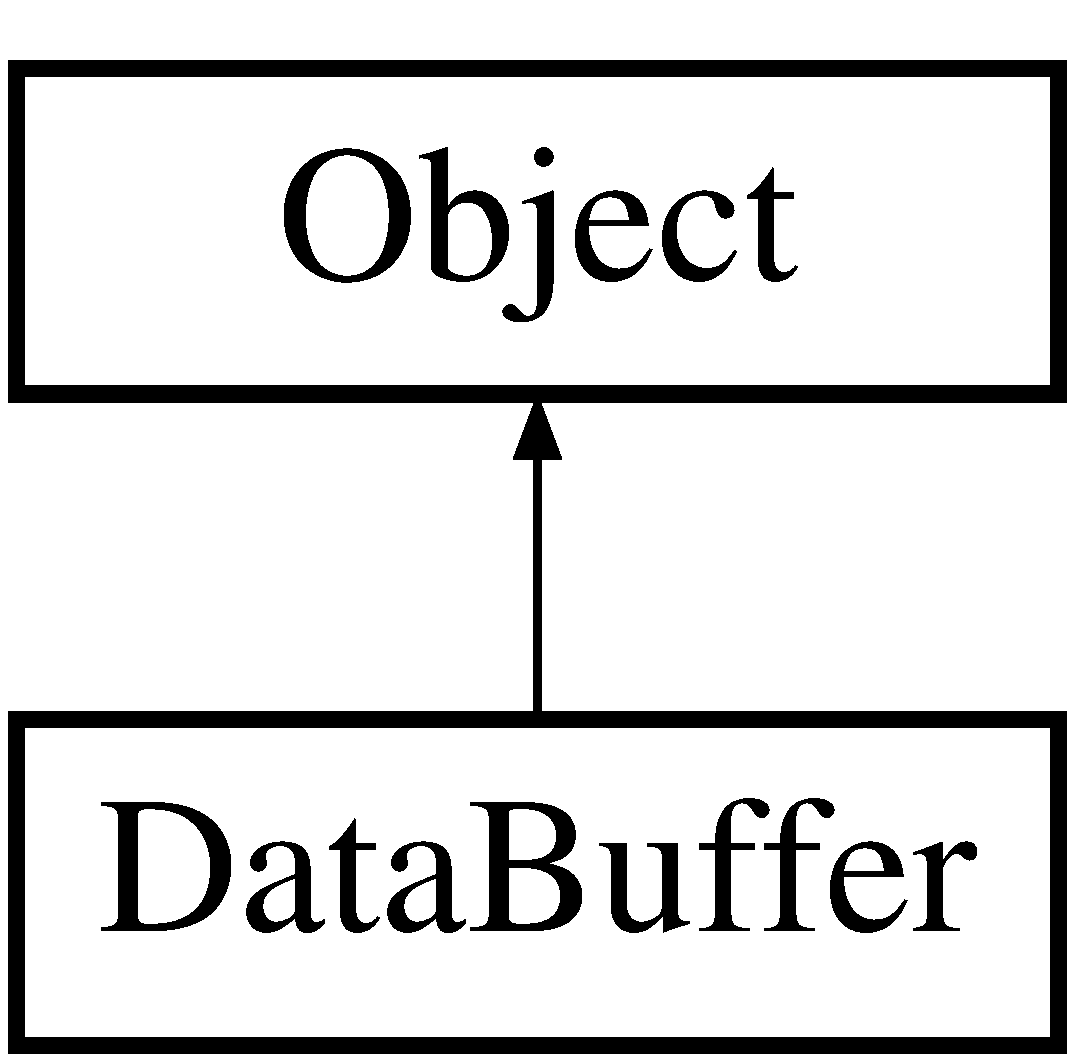
\includegraphics[height=2.000000cm]{class_data_buffer}
\end{center}
\end{figure}
\subsection*{Public Member Functions}
\begin{DoxyCompactItemize}
\item 
\hyperlink{class_data_buffer_ad12238b0a14ce03f1f2812fd8ce9adf4}{Data\+Buffer} (I\+D3\+D11\+Device $\ast$dx\+Device, D3\+D11\+\_\+\+B\+I\+N\+D\+\_\+\+F\+L\+AG bind\+Flags, const void $\ast$buffer, size\+\_\+t size)
\begin{DoxyCompactList}\small\item\em Constructor. \end{DoxyCompactList}\item 
virtual \hyperlink{class_data_buffer_ac374f86810cc019a248be28d1babecdb}{$\sim$\+Data\+Buffer} ()
\begin{DoxyCompactList}\small\item\em Destructor. \end{DoxyCompactList}\item 
I\+D3\+D11\+Buffer $\ast$\& \hyperlink{class_data_buffer_a282a755677be1eac733f3e1e090e6069}{Get\+Dx\+Buffer} ()
\begin{DoxyCompactList}\small\item\em Getters. \end{DoxyCompactList}\item 
D3\+D11\+\_\+\+B\+U\+F\+F\+E\+R\+\_\+\+D\+E\+SC \hyperlink{class_data_buffer_a1012af5db0fb0dbc042a4d7ddc3d8249}{Get\+Dx\+Buffer\+Description} ()
\item 
D3\+D11\+\_\+\+S\+U\+B\+R\+E\+S\+O\+U\+R\+C\+E\+\_\+\+D\+A\+TA \hyperlink{class_data_buffer_a385e821a26a26326d22d92f7e9268469}{Get\+Dx\+Sub\+Resource\+Data} ()
\item 
size\+\_\+t \hyperlink{class_data_buffer_aaa2b70d7c6cc014e9ccd7e949ecbbf38}{Get\+Size} ()
\end{DoxyCompactItemize}
\subsection*{Protected Attributes}
\begin{DoxyCompactItemize}
\item 
D3\+D11\+\_\+\+B\+U\+F\+F\+E\+R\+\_\+\+D\+E\+SC \hyperlink{class_data_buffer_aca633d446c9c237966a06baca5df245d}{my\+Dx\+Buffer\+Description}
\item 
D3\+D11\+\_\+\+S\+U\+B\+R\+E\+S\+O\+U\+R\+C\+E\+\_\+\+D\+A\+TA \hyperlink{class_data_buffer_a20ae63eb53988ea2963b45a307615d39}{my\+Dx\+Sub\+Resource\+Data}
\item 
I\+D3\+D11\+Buffer $\ast$ \hyperlink{class_data_buffer_a3bea6da94472c8b55032713ec8463853}{my\+Dx\+Buffer}
\item 
size\+\_\+t \hyperlink{class_data_buffer_a31bb760d7d272d637e387b37d7caecfe}{my\+Size}
\end{DoxyCompactItemize}
\subsection*{Additional Inherited Members}


\subsection{Constructor \& Destructor Documentation}
\index{Data\+Buffer@{Data\+Buffer}!Data\+Buffer@{Data\+Buffer}}
\index{Data\+Buffer@{Data\+Buffer}!Data\+Buffer@{Data\+Buffer}}
\subsubsection[{\texorpdfstring{Data\+Buffer(\+I\+D3\+D11\+Device $\ast$dx\+Device, D3\+D11\+\_\+\+B\+I\+N\+D\+\_\+\+F\+L\+A\+G bind\+Flags, const void $\ast$buffer, size\+\_\+t size)}{DataBuffer(ID3D11Device *dxDevice, D3D11_BIND_FLAG bindFlags, const void *buffer, size_t size)}}]{\setlength{\rightskip}{0pt plus 5cm}Data\+Buffer\+::\+Data\+Buffer (
\begin{DoxyParamCaption}
\item[{I\+D3\+D11\+Device $\ast$}]{dx\+Device, }
\item[{D3\+D11\+\_\+\+B\+I\+N\+D\+\_\+\+F\+L\+AG}]{bind\+Flags, }
\item[{const void $\ast$}]{buffer, }
\item[{size\+\_\+t}]{size}
\end{DoxyParamCaption}
)}\hypertarget{class_data_buffer_ad12238b0a14ce03f1f2812fd8ce9adf4}{}\label{class_data_buffer_ad12238b0a14ce03f1f2812fd8ce9adf4}


Constructor. 

Constructor, Creates a DirextX Buffer -\/ used for passing data to the shader among other things.

\begin{DoxyAuthor}{Author}
Katianie 
\end{DoxyAuthor}
\begin{DoxyDate}{Date}
7/4/2016
\end{DoxyDate}

\begin{DoxyParams}[1]{Parameters}
\mbox{\tt in}  & {\em dx\+Device} & The DX Device. \\
\hline
 & {\em bind\+Flags} & The bind flags. \\
\hline
 & {\em buffer} & The data for the buffer. \\
\hline
 & {\em size} & The byte width. \\
\hline
\end{DoxyParams}
\index{Data\+Buffer@{Data\+Buffer}!````~Data\+Buffer@{$\sim$\+Data\+Buffer}}
\index{````~Data\+Buffer@{$\sim$\+Data\+Buffer}!Data\+Buffer@{Data\+Buffer}}
\subsubsection[{\texorpdfstring{$\sim$\+Data\+Buffer()}{~DataBuffer()}}]{\setlength{\rightskip}{0pt plus 5cm}Data\+Buffer\+::$\sim$\+Data\+Buffer (
\begin{DoxyParamCaption}
{}
\end{DoxyParamCaption}
)\hspace{0.3cm}{\ttfamily [virtual]}}\hypertarget{class_data_buffer_ac374f86810cc019a248be28d1babecdb}{}\label{class_data_buffer_ac374f86810cc019a248be28d1babecdb}


Destructor. 

Destructor.

\begin{DoxyAuthor}{Author}
Katianie 
\end{DoxyAuthor}
\begin{DoxyDate}{Date}
7/4/2016 
\end{DoxyDate}


\subsection{Member Function Documentation}
\index{Data\+Buffer@{Data\+Buffer}!Get\+Dx\+Buffer@{Get\+Dx\+Buffer}}
\index{Get\+Dx\+Buffer@{Get\+Dx\+Buffer}!Data\+Buffer@{Data\+Buffer}}
\subsubsection[{\texorpdfstring{Get\+Dx\+Buffer()}{GetDxBuffer()}}]{\setlength{\rightskip}{0pt plus 5cm}I\+D3\+D11\+Buffer $\ast$\& Data\+Buffer\+::\+Get\+Dx\+Buffer (
\begin{DoxyParamCaption}
{}
\end{DoxyParamCaption}
)}\hypertarget{class_data_buffer_a282a755677be1eac733f3e1e090e6069}{}\label{class_data_buffer_a282a755677be1eac733f3e1e090e6069}


Getters. 

Gets the DX Buffer.

\begin{DoxyAuthor}{Author}
Katianie 
\end{DoxyAuthor}
\begin{DoxyDate}{Date}
7/4/2016
\end{DoxyDate}
\begin{DoxyReturn}{Returns}
The DX Buffer. 
\end{DoxyReturn}
\index{Data\+Buffer@{Data\+Buffer}!Get\+Dx\+Buffer\+Description@{Get\+Dx\+Buffer\+Description}}
\index{Get\+Dx\+Buffer\+Description@{Get\+Dx\+Buffer\+Description}!Data\+Buffer@{Data\+Buffer}}
\subsubsection[{\texorpdfstring{Get\+Dx\+Buffer\+Description()}{GetDxBufferDescription()}}]{\setlength{\rightskip}{0pt plus 5cm}D3\+D11\+\_\+\+B\+U\+F\+F\+E\+R\+\_\+\+D\+E\+SC Data\+Buffer\+::\+Get\+Dx\+Buffer\+Description (
\begin{DoxyParamCaption}
{}
\end{DoxyParamCaption}
)}\hypertarget{class_data_buffer_a1012af5db0fb0dbc042a4d7ddc3d8249}{}\label{class_data_buffer_a1012af5db0fb0dbc042a4d7ddc3d8249}
Gets the DX Buffer Description.

\begin{DoxyAuthor}{Author}
Katianie 
\end{DoxyAuthor}
\begin{DoxyDate}{Date}
7/4/2016
\end{DoxyDate}
\begin{DoxyReturn}{Returns}
The DX Buffer Description. 
\end{DoxyReturn}
\index{Data\+Buffer@{Data\+Buffer}!Get\+Dx\+Sub\+Resource\+Data@{Get\+Dx\+Sub\+Resource\+Data}}
\index{Get\+Dx\+Sub\+Resource\+Data@{Get\+Dx\+Sub\+Resource\+Data}!Data\+Buffer@{Data\+Buffer}}
\subsubsection[{\texorpdfstring{Get\+Dx\+Sub\+Resource\+Data()}{GetDxSubResourceData()}}]{\setlength{\rightskip}{0pt plus 5cm}D3\+D11\+\_\+\+S\+U\+B\+R\+E\+S\+O\+U\+R\+C\+E\+\_\+\+D\+A\+TA Data\+Buffer\+::\+Get\+Dx\+Sub\+Resource\+Data (
\begin{DoxyParamCaption}
{}
\end{DoxyParamCaption}
)}\hypertarget{class_data_buffer_a385e821a26a26326d22d92f7e9268469}{}\label{class_data_buffer_a385e821a26a26326d22d92f7e9268469}
Gets the DX Sub Resource Data.

\begin{DoxyAuthor}{Author}
Katianie 
\end{DoxyAuthor}
\begin{DoxyDate}{Date}
7/4/2016
\end{DoxyDate}
\begin{DoxyReturn}{Returns}
The DX Sub Resource Data. 
\end{DoxyReturn}
\index{Data\+Buffer@{Data\+Buffer}!Get\+Size@{Get\+Size}}
\index{Get\+Size@{Get\+Size}!Data\+Buffer@{Data\+Buffer}}
\subsubsection[{\texorpdfstring{Get\+Size()}{GetSize()}}]{\setlength{\rightskip}{0pt plus 5cm}size\+\_\+t Data\+Buffer\+::\+Get\+Size (
\begin{DoxyParamCaption}
{}
\end{DoxyParamCaption}
)}\hypertarget{class_data_buffer_aaa2b70d7c6cc014e9ccd7e949ecbbf38}{}\label{class_data_buffer_aaa2b70d7c6cc014e9ccd7e949ecbbf38}
Gets the size of the Buffer.

\begin{DoxyAuthor}{Author}
Katianie 
\end{DoxyAuthor}
\begin{DoxyDate}{Date}
7/4/2016
\end{DoxyDate}
\begin{DoxyReturn}{Returns}
The size of the Buffer. 
\end{DoxyReturn}


\subsection{Member Data Documentation}
\index{Data\+Buffer@{Data\+Buffer}!my\+Dx\+Buffer@{my\+Dx\+Buffer}}
\index{my\+Dx\+Buffer@{my\+Dx\+Buffer}!Data\+Buffer@{Data\+Buffer}}
\subsubsection[{\texorpdfstring{my\+Dx\+Buffer}{myDxBuffer}}]{\setlength{\rightskip}{0pt plus 5cm}I\+D3\+D11\+Buffer$\ast$ Data\+Buffer\+::my\+Dx\+Buffer\hspace{0.3cm}{\ttfamily [protected]}}\hypertarget{class_data_buffer_a3bea6da94472c8b55032713ec8463853}{}\label{class_data_buffer_a3bea6da94472c8b55032713ec8463853}
\index{Data\+Buffer@{Data\+Buffer}!my\+Dx\+Buffer\+Description@{my\+Dx\+Buffer\+Description}}
\index{my\+Dx\+Buffer\+Description@{my\+Dx\+Buffer\+Description}!Data\+Buffer@{Data\+Buffer}}
\subsubsection[{\texorpdfstring{my\+Dx\+Buffer\+Description}{myDxBufferDescription}}]{\setlength{\rightskip}{0pt plus 5cm}D3\+D11\+\_\+\+B\+U\+F\+F\+E\+R\+\_\+\+D\+E\+SC Data\+Buffer\+::my\+Dx\+Buffer\+Description\hspace{0.3cm}{\ttfamily [protected]}}\hypertarget{class_data_buffer_aca633d446c9c237966a06baca5df245d}{}\label{class_data_buffer_aca633d446c9c237966a06baca5df245d}
\index{Data\+Buffer@{Data\+Buffer}!my\+Dx\+Sub\+Resource\+Data@{my\+Dx\+Sub\+Resource\+Data}}
\index{my\+Dx\+Sub\+Resource\+Data@{my\+Dx\+Sub\+Resource\+Data}!Data\+Buffer@{Data\+Buffer}}
\subsubsection[{\texorpdfstring{my\+Dx\+Sub\+Resource\+Data}{myDxSubResourceData}}]{\setlength{\rightskip}{0pt plus 5cm}D3\+D11\+\_\+\+S\+U\+B\+R\+E\+S\+O\+U\+R\+C\+E\+\_\+\+D\+A\+TA Data\+Buffer\+::my\+Dx\+Sub\+Resource\+Data\hspace{0.3cm}{\ttfamily [protected]}}\hypertarget{class_data_buffer_a20ae63eb53988ea2963b45a307615d39}{}\label{class_data_buffer_a20ae63eb53988ea2963b45a307615d39}
\index{Data\+Buffer@{Data\+Buffer}!my\+Size@{my\+Size}}
\index{my\+Size@{my\+Size}!Data\+Buffer@{Data\+Buffer}}
\subsubsection[{\texorpdfstring{my\+Size}{mySize}}]{\setlength{\rightskip}{0pt plus 5cm}size\+\_\+t Data\+Buffer\+::my\+Size\hspace{0.3cm}{\ttfamily [protected]}}\hypertarget{class_data_buffer_a31bb760d7d272d637e387b37d7caecfe}{}\label{class_data_buffer_a31bb760d7d272d637e387b37d7caecfe}


The documentation for this class was generated from the following files\+:\begin{DoxyCompactItemize}
\item 
Samples/\+Oculus\+Room\+Tiny\+\_\+\+Advanced/\+Common/\+Headers/\hyperlink{_data_buffer_8h}{Data\+Buffer.\+h}\item 
Samples/\+Oculus\+Room\+Tiny\+\_\+\+Advanced/\+Common/\+Implementations/\hyperlink{_data_buffer_8cpp}{Data\+Buffer.\+cpp}\end{DoxyCompactItemize}

\hypertarget{class_depth_buffer}{}\section{Depth\+Buffer Class Reference}
\label{class_depth_buffer}\index{Depth\+Buffer@{Depth\+Buffer}}


{\ttfamily \#include $<$Depth\+Buffer.\+h$>$}

Inheritance diagram for Depth\+Buffer\+:\begin{figure}[H]
\begin{center}
\leavevmode
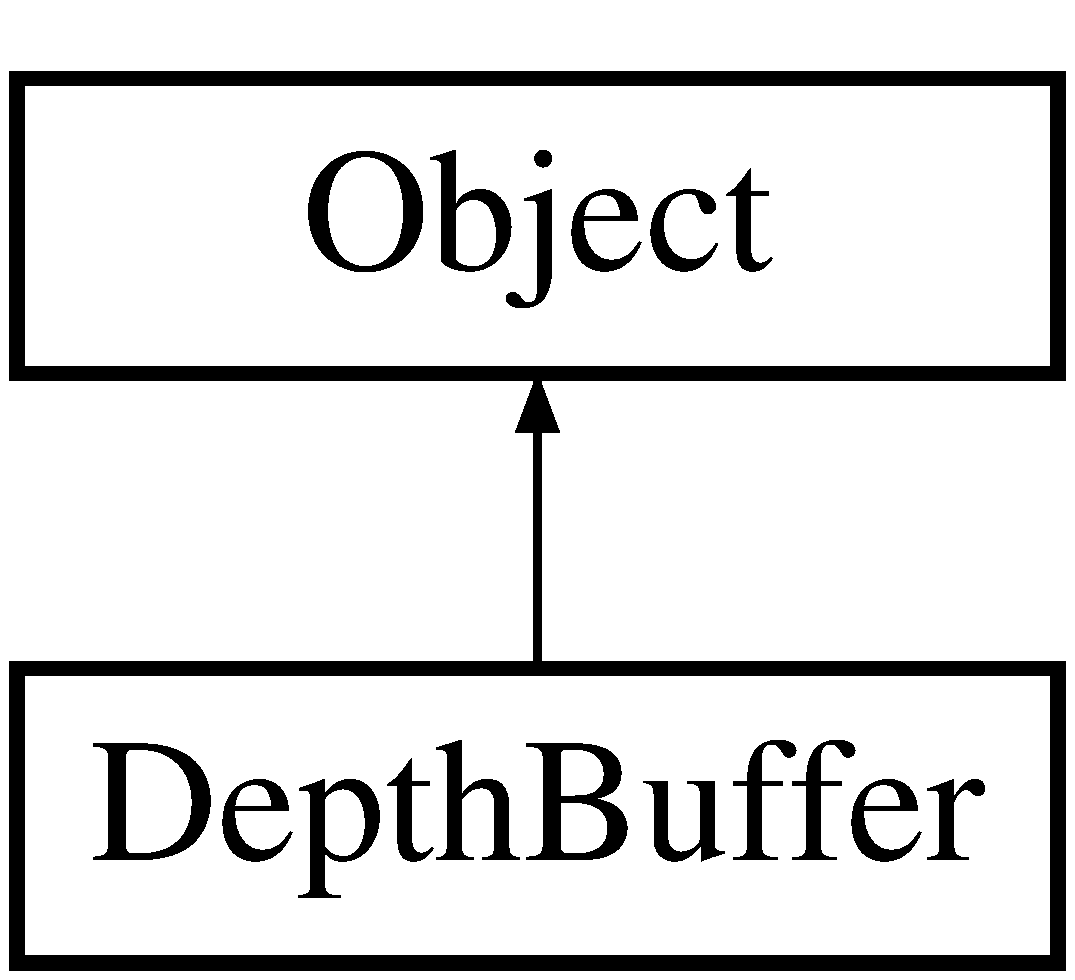
\includegraphics[height=2.000000cm]{class_depth_buffer}
\end{center}
\end{figure}
\subsection*{Public Member Functions}
\begin{DoxyCompactItemize}
\item 
\hyperlink{class_depth_buffer_aa5c885f142495745de6e4d4595987dc4}{Depth\+Buffer} (I\+D3\+D11\+Device $\ast$dx\+Device, int window\+Width, int window\+Height, int sample\+Count=1)
\begin{DoxyCompactList}\small\item\em Constructor. \end{DoxyCompactList}\item 
virtual \hyperlink{class_depth_buffer_a9d04ef2a88a2414d476f4fc27a25a7a8}{$\sim$\+Depth\+Buffer} ()
\begin{DoxyCompactList}\small\item\em Destructor. \end{DoxyCompactList}\item 
D\+X\+G\+I\+\_\+\+F\+O\+R\+M\+AT \hyperlink{class_depth_buffer_aa72fe3a246f368d405ff2666c4e150fa}{Get\+Dx\+Format} ()
\begin{DoxyCompactList}\small\item\em Getters. \end{DoxyCompactList}\item 
I\+D3\+D11\+Texture2D $\ast$ \hyperlink{class_depth_buffer_ad3b4f85ced7bb00beea9ac63b0b34774}{Get\+Dx\+Texture} ()
\item 
I\+D3\+D11\+Depth\+Stencil\+View $\ast$ \hyperlink{class_depth_buffer_ad5ff6602f8b18faf2010297e677815ec}{Get\+Dx\+Texture\+Depth\+Stencil\+View} ()
\item 
D3\+D11\+\_\+\+T\+E\+X\+T\+U\+R\+E2\+D\+\_\+\+D\+E\+SC \hyperlink{class_depth_buffer_aedd68b34c8aedb0f8826a89a0b3f19a8}{Get\+Dx\+Texture\+Description} ()
\end{DoxyCompactItemize}
\subsection*{Protected Attributes}
\begin{DoxyCompactItemize}
\item 
I\+D3\+D11\+Depth\+Stencil\+View $\ast$ \hyperlink{class_depth_buffer_a6f9f968908fcf216ea38e9b8618853ef}{my\+Dx\+Texture\+Depth\+Stencil\+View}
\item 
I\+D3\+D11\+Texture2D $\ast$ \hyperlink{class_depth_buffer_a2ba736f2db94d8491cce355635051d51}{my\+Dx\+Texture}
\item 
D\+X\+G\+I\+\_\+\+F\+O\+R\+M\+AT \hyperlink{class_depth_buffer_a6ec2773387e954b6db05500b2247d5c2}{my\+Dx\+Format} = D\+X\+G\+I\+\_\+\+F\+O\+R\+M\+A\+T\+\_\+\+D32\+\_\+\+F\+L\+O\+AT
\item 
D3\+D11\+\_\+\+T\+E\+X\+T\+U\+R\+E2\+D\+\_\+\+D\+E\+SC \hyperlink{class_depth_buffer_a217ff5c9e8c6c7609626a81cf704dd1d}{my\+Dx\+Texture\+Description}
\end{DoxyCompactItemize}
\subsection*{Additional Inherited Members}


\subsection{Constructor \& Destructor Documentation}
\index{Depth\+Buffer@{Depth\+Buffer}!Depth\+Buffer@{Depth\+Buffer}}
\index{Depth\+Buffer@{Depth\+Buffer}!Depth\+Buffer@{Depth\+Buffer}}
\subsubsection[{\texorpdfstring{Depth\+Buffer(\+I\+D3\+D11\+Device $\ast$dx\+Device, int window\+Width, int window\+Height, int sample\+Count=1)}{DepthBuffer(ID3D11Device *dxDevice, int windowWidth, int windowHeight, int sampleCount=1)}}]{\setlength{\rightskip}{0pt plus 5cm}Depth\+Buffer\+::\+Depth\+Buffer (
\begin{DoxyParamCaption}
\item[{I\+D3\+D11\+Device $\ast$}]{dx\+Device, }
\item[{int}]{window\+Width, }
\item[{int}]{window\+Height, }
\item[{int}]{sample\+Count = {\ttfamily 1}}
\end{DoxyParamCaption}
)}\hypertarget{class_depth_buffer_aa5c885f142495745de6e4d4595987dc4}{}\label{class_depth_buffer_aa5c885f142495745de6e4d4595987dc4}


Constructor. 

Constructor, initializes buffer to store Z order data aka Z-\/\+Buffer.

\begin{DoxyAuthor}{Author}
Katianie 
\end{DoxyAuthor}
\begin{DoxyDate}{Date}
7/4/2016
\end{DoxyDate}

\begin{DoxyParams}[1]{Parameters}
\mbox{\tt in,out}  & {\em dx\+Device} & The DX Device. \\
\hline
 & {\em window\+Width} & The width of the window. \\
\hline
 & {\em window\+Height} & The height of the window. \\
\hline
 & {\em sample\+Count} & Number of samples. \\
\hline
\end{DoxyParams}
\index{Depth\+Buffer@{Depth\+Buffer}!````~Depth\+Buffer@{$\sim$\+Depth\+Buffer}}
\index{````~Depth\+Buffer@{$\sim$\+Depth\+Buffer}!Depth\+Buffer@{Depth\+Buffer}}
\subsubsection[{\texorpdfstring{$\sim$\+Depth\+Buffer()}{~DepthBuffer()}}]{\setlength{\rightskip}{0pt plus 5cm}Depth\+Buffer\+::$\sim$\+Depth\+Buffer (
\begin{DoxyParamCaption}
{}
\end{DoxyParamCaption}
)\hspace{0.3cm}{\ttfamily [virtual]}}\hypertarget{class_depth_buffer_a9d04ef2a88a2414d476f4fc27a25a7a8}{}\label{class_depth_buffer_a9d04ef2a88a2414d476f4fc27a25a7a8}


Destructor. 

Destructor.

\begin{DoxyAuthor}{Author}
Katianie 
\end{DoxyAuthor}
\begin{DoxyDate}{Date}
7/4/2016 
\end{DoxyDate}


\subsection{Member Function Documentation}
\index{Depth\+Buffer@{Depth\+Buffer}!Get\+Dx\+Format@{Get\+Dx\+Format}}
\index{Get\+Dx\+Format@{Get\+Dx\+Format}!Depth\+Buffer@{Depth\+Buffer}}
\subsubsection[{\texorpdfstring{Get\+Dx\+Format()}{GetDxFormat()}}]{\setlength{\rightskip}{0pt plus 5cm}D\+X\+G\+I\+\_\+\+F\+O\+R\+M\+AT Depth\+Buffer\+::\+Get\+Dx\+Format (
\begin{DoxyParamCaption}
{}
\end{DoxyParamCaption}
)}\hypertarget{class_depth_buffer_aa72fe3a246f368d405ff2666c4e150fa}{}\label{class_depth_buffer_aa72fe3a246f368d405ff2666c4e150fa}


Getters. 

Gets the DX Format.

\begin{DoxyAuthor}{Author}
Katianie 
\end{DoxyAuthor}
\begin{DoxyDate}{Date}
7/4/2016
\end{DoxyDate}
\begin{DoxyReturn}{Returns}
The DX Format. 
\end{DoxyReturn}
\index{Depth\+Buffer@{Depth\+Buffer}!Get\+Dx\+Texture@{Get\+Dx\+Texture}}
\index{Get\+Dx\+Texture@{Get\+Dx\+Texture}!Depth\+Buffer@{Depth\+Buffer}}
\subsubsection[{\texorpdfstring{Get\+Dx\+Texture()}{GetDxTexture()}}]{\setlength{\rightskip}{0pt plus 5cm}I\+D3\+D11\+Texture2D $\ast$ Depth\+Buffer\+::\+Get\+Dx\+Texture (
\begin{DoxyParamCaption}
{}
\end{DoxyParamCaption}
)}\hypertarget{class_depth_buffer_ad3b4f85ced7bb00beea9ac63b0b34774}{}\label{class_depth_buffer_ad3b4f85ced7bb00beea9ac63b0b34774}
Gets the DX \hyperlink{class_texture}{Texture}.

\begin{DoxyAuthor}{Author}
Katianie 
\end{DoxyAuthor}
\begin{DoxyDate}{Date}
7/4/2016
\end{DoxyDate}
\begin{DoxyReturn}{Returns}
the DX \hyperlink{class_texture}{Texture}. 
\end{DoxyReturn}
\index{Depth\+Buffer@{Depth\+Buffer}!Get\+Dx\+Texture\+Depth\+Stencil\+View@{Get\+Dx\+Texture\+Depth\+Stencil\+View}}
\index{Get\+Dx\+Texture\+Depth\+Stencil\+View@{Get\+Dx\+Texture\+Depth\+Stencil\+View}!Depth\+Buffer@{Depth\+Buffer}}
\subsubsection[{\texorpdfstring{Get\+Dx\+Texture\+Depth\+Stencil\+View()}{GetDxTextureDepthStencilView()}}]{\setlength{\rightskip}{0pt plus 5cm}I\+D3\+D11\+Depth\+Stencil\+View $\ast$ Depth\+Buffer\+::\+Get\+Dx\+Texture\+Depth\+Stencil\+View (
\begin{DoxyParamCaption}
{}
\end{DoxyParamCaption}
)}\hypertarget{class_depth_buffer_ad5ff6602f8b18faf2010297e677815ec}{}\label{class_depth_buffer_ad5ff6602f8b18faf2010297e677815ec}
Gets the DX \hyperlink{class_texture}{Texture} Depth Stencil View.

\begin{DoxyAuthor}{Author}
Katianie 
\end{DoxyAuthor}
\begin{DoxyDate}{Date}
7/4/2016
\end{DoxyDate}
\begin{DoxyReturn}{Returns}
The DX \hyperlink{class_texture}{Texture} Depth Stencil View. 
\end{DoxyReturn}
\index{Depth\+Buffer@{Depth\+Buffer}!Get\+Dx\+Texture\+Description@{Get\+Dx\+Texture\+Description}}
\index{Get\+Dx\+Texture\+Description@{Get\+Dx\+Texture\+Description}!Depth\+Buffer@{Depth\+Buffer}}
\subsubsection[{\texorpdfstring{Get\+Dx\+Texture\+Description()}{GetDxTextureDescription()}}]{\setlength{\rightskip}{0pt plus 5cm}D3\+D11\+\_\+\+T\+E\+X\+T\+U\+R\+E2\+D\+\_\+\+D\+E\+SC Depth\+Buffer\+::\+Get\+Dx\+Texture\+Description (
\begin{DoxyParamCaption}
{}
\end{DoxyParamCaption}
)}\hypertarget{class_depth_buffer_aedd68b34c8aedb0f8826a89a0b3f19a8}{}\label{class_depth_buffer_aedd68b34c8aedb0f8826a89a0b3f19a8}
Gets the DX \hyperlink{class_texture}{Texture} Description.

\begin{DoxyAuthor}{Author}
Katianie 
\end{DoxyAuthor}
\begin{DoxyDate}{Date}
7/4/2016
\end{DoxyDate}
\begin{DoxyReturn}{Returns}
The DX \hyperlink{class_texture}{Texture} Description. 
\end{DoxyReturn}


\subsection{Member Data Documentation}
\index{Depth\+Buffer@{Depth\+Buffer}!my\+Dx\+Format@{my\+Dx\+Format}}
\index{my\+Dx\+Format@{my\+Dx\+Format}!Depth\+Buffer@{Depth\+Buffer}}
\subsubsection[{\texorpdfstring{my\+Dx\+Format}{myDxFormat}}]{\setlength{\rightskip}{0pt plus 5cm}D\+X\+G\+I\+\_\+\+F\+O\+R\+M\+AT Depth\+Buffer\+::my\+Dx\+Format = D\+X\+G\+I\+\_\+\+F\+O\+R\+M\+A\+T\+\_\+\+D32\+\_\+\+F\+L\+O\+AT\hspace{0.3cm}{\ttfamily [protected]}}\hypertarget{class_depth_buffer_a6ec2773387e954b6db05500b2247d5c2}{}\label{class_depth_buffer_a6ec2773387e954b6db05500b2247d5c2}
\index{Depth\+Buffer@{Depth\+Buffer}!my\+Dx\+Texture@{my\+Dx\+Texture}}
\index{my\+Dx\+Texture@{my\+Dx\+Texture}!Depth\+Buffer@{Depth\+Buffer}}
\subsubsection[{\texorpdfstring{my\+Dx\+Texture}{myDxTexture}}]{\setlength{\rightskip}{0pt plus 5cm}I\+D3\+D11\+Texture2D$\ast$ Depth\+Buffer\+::my\+Dx\+Texture\hspace{0.3cm}{\ttfamily [protected]}}\hypertarget{class_depth_buffer_a2ba736f2db94d8491cce355635051d51}{}\label{class_depth_buffer_a2ba736f2db94d8491cce355635051d51}
\index{Depth\+Buffer@{Depth\+Buffer}!my\+Dx\+Texture\+Depth\+Stencil\+View@{my\+Dx\+Texture\+Depth\+Stencil\+View}}
\index{my\+Dx\+Texture\+Depth\+Stencil\+View@{my\+Dx\+Texture\+Depth\+Stencil\+View}!Depth\+Buffer@{Depth\+Buffer}}
\subsubsection[{\texorpdfstring{my\+Dx\+Texture\+Depth\+Stencil\+View}{myDxTextureDepthStencilView}}]{\setlength{\rightskip}{0pt plus 5cm}I\+D3\+D11\+Depth\+Stencil\+View$\ast$ Depth\+Buffer\+::my\+Dx\+Texture\+Depth\+Stencil\+View\hspace{0.3cm}{\ttfamily [protected]}}\hypertarget{class_depth_buffer_a6f9f968908fcf216ea38e9b8618853ef}{}\label{class_depth_buffer_a6f9f968908fcf216ea38e9b8618853ef}
\index{Depth\+Buffer@{Depth\+Buffer}!my\+Dx\+Texture\+Description@{my\+Dx\+Texture\+Description}}
\index{my\+Dx\+Texture\+Description@{my\+Dx\+Texture\+Description}!Depth\+Buffer@{Depth\+Buffer}}
\subsubsection[{\texorpdfstring{my\+Dx\+Texture\+Description}{myDxTextureDescription}}]{\setlength{\rightskip}{0pt plus 5cm}D3\+D11\+\_\+\+T\+E\+X\+T\+U\+R\+E2\+D\+\_\+\+D\+E\+SC Depth\+Buffer\+::my\+Dx\+Texture\+Description\hspace{0.3cm}{\ttfamily [protected]}}\hypertarget{class_depth_buffer_a217ff5c9e8c6c7609626a81cf704dd1d}{}\label{class_depth_buffer_a217ff5c9e8c6c7609626a81cf704dd1d}


The documentation for this class was generated from the following files\+:\begin{DoxyCompactItemize}
\item 
Samples/\+Oculus\+Room\+Tiny\+\_\+\+Advanced/\+Common/\+Headers/\hyperlink{_depth_buffer_8h}{Depth\+Buffer.\+h}\item 
Samples/\+Oculus\+Room\+Tiny\+\_\+\+Advanced/\+Common/\+Implementations/\hyperlink{_depth_buffer_8cpp}{Depth\+Buffer.\+cpp}\end{DoxyCompactItemize}

\hypertarget{class_direct_x_manager}{}\section{Direct\+X\+Manager Class Reference}
\label{class_direct_x_manager}\index{Direct\+X\+Manager@{Direct\+X\+Manager}}


{\ttfamily \#include $<$Direct\+X\+Manager.\+h$>$}

Inheritance diagram for Direct\+X\+Manager\+:\begin{figure}[H]
\begin{center}
\leavevmode
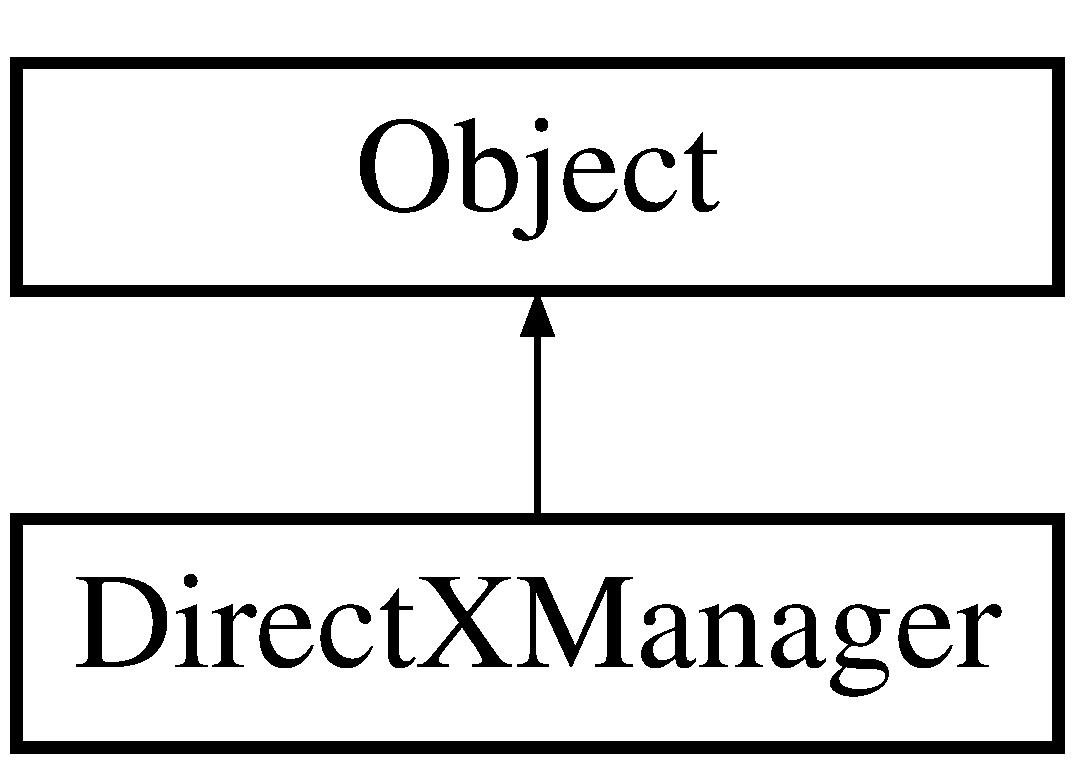
\includegraphics[height=2.000000cm]{class_direct_x_manager}
\end{center}
\end{figure}
\subsection*{Public Member Functions}
\begin{DoxyCompactItemize}
\item 
virtual \hyperlink{class_direct_x_manager_a5c9ef465fa2eed372c462fe34fa6a0d1}{$\sim$\+Direct\+X\+Manager} ()
\begin{DoxyCompactList}\small\item\em Destructor. \end{DoxyCompactList}\item 
void \hyperlink{class_direct_x_manager_a50fbe9ef22a71b8d56599735d6b813d9}{Close\+Window} ()
\begin{DoxyCompactList}\small\item\em Functions. \end{DoxyCompactList}\item 
bool \hyperlink{class_direct_x_manager_afc1e06766269d5535ba71c542acdc8e8}{Handle\+Messages} ()
\item 
bool \hyperlink{class_direct_x_manager_a4314d94fefe4c2eec896c45c8cc5a77e}{Init\+Device} (int viewport\+Width, int viewport\+Height, const L\+U\+ID $\ast$p\+Luid, bool is\+Windowed=true)
\item 
void \hyperlink{class_direct_x_manager_a7226059ce9d4970d17cb4924058eb9f2}{Init\+Viewport} (float viewportX, float viewportY, float viewport\+Width, float viewport\+Height)
\item 
bool \hyperlink{class_direct_x_manager_ada12791447237c01bd511c3c6bf822e8}{Init\+Window} (H\+I\+N\+S\+T\+A\+N\+CE h\+Instance, L\+P\+C\+W\+S\+TR title)
\item 
void \hyperlink{class_direct_x_manager_a2d8ffc338f3520548e7fc0ea573b686e}{Release\+Device} ()
\item 
void \hyperlink{class_direct_x_manager_af2bbed3ede3068ae5679632b1c739165}{Set\+And\+Clear\+Render\+Target} (I\+D3\+D11\+Render\+Target\+View $\ast$rendertarget, \hyperlink{class_depth_buffer}{Depth\+Buffer} $\ast$depthbuffer, float R=0.\+0f, float G=0.\+0f, float B=0.\+0f, float A=0.\+0f)
\item 
I\+D3\+D11\+Render\+Target\+View $\ast$ \hyperlink{class_direct_x_manager_a99b3f77cccd824c62979affb01775b68}{Get\+Dx\+Back\+Buffer\+Render\+Target} ()
\begin{DoxyCompactList}\small\item\em Getters. \end{DoxyCompactList}\item 
I\+D3\+D11\+Texture2D $\ast$ \hyperlink{class_direct_x_manager_a99ac3db0b44425089a176fc741b4726d}{Get\+Dx\+Back\+Buffer\+Texture} ()
\item 
I\+D3\+D11\+Device $\ast$ \hyperlink{class_direct_x_manager_abb96057eb5bf224ef98060bd34b48751}{Get\+Dx\+Device} ()
\item 
I\+D3\+D11\+Device\+Context $\ast$ \hyperlink{class_direct_x_manager_ae9c3888bc7917e6ea3259d7816fe108a}{Get\+Dx\+Device\+Context} ()
\item 
I\+D\+X\+G\+I\+Swap\+Chain $\ast$ \hyperlink{class_direct_x_manager_a310a11a8113c758033f6b73fdde53030}{Get\+Dx\+Swap\+Chain} ()
\item 
H\+I\+N\+S\+T\+A\+N\+CE \hyperlink{class_direct_x_manager_a9cc5d9f93f5c2527db03de9dfe39bddf}{Get\+H\+Instance} ()
\item 
bool \hyperlink{class_direct_x_manager_a4270aa51fbde3ca7257e2904972a606b}{Get\+Is\+Running} ()
\item 
\hyperlink{class_depth_buffer}{Depth\+Buffer} $\ast$ \hyperlink{class_direct_x_manager_abf6b3476bf3f3e93a15d878d3fb0d96c}{Get\+Main\+Depth\+Buffer} ()
\item 
unsigned char $\ast$ \hyperlink{class_direct_x_manager_a3f0de0a051dbb65f80eb1f947d00c4cd}{Get\+Uniform\+Data} ()
\item 
\hyperlink{class_data_buffer}{Data\+Buffer} $\ast$ \hyperlink{class_direct_x_manager_a3ecf250110570278558a06be31c98837}{Get\+Uniform\+Data\+Buffer} ()
\item 
H\+W\+ND \hyperlink{class_direct_x_manager_a51978215008055fa610f4eafd39fd8f8}{Get\+Window} ()
\item 
int \hyperlink{class_direct_x_manager_a49d8a5684c325e88886e5fa5e1d83089}{Get\+Window\+Size\+Height} ()
\item 
int \hyperlink{class_direct_x_manager_aebaff0bb77f5b660ec5ea25b7a131229}{Get\+Window\+Size\+Width} ()
\item 
void \hyperlink{class_direct_x_manager_aae3c1e2ebb395bfec27e2f15ed6b8c80}{Set\+Uniform\+Data} (int offset, const void $\ast$data, int size)
\begin{DoxyCompactList}\small\item\em Setters. \end{DoxyCompactList}\end{DoxyCompactItemize}
\subsection*{Static Public Member Functions}
\begin{DoxyCompactItemize}
\item 
static \hyperlink{class_direct_x_manager}{Direct\+X\+Manager} \& \hyperlink{class_direct_x_manager_ac785f35f30dd23faa97ec028ff2a4c91}{Retrieve\+Direct\+X\+Manager} ()
\begin{DoxyCompactList}\small\item\em Singleton Constructor/\+Getter. \end{DoxyCompactList}\item 
static L\+R\+E\+S\+U\+LT C\+A\+L\+L\+B\+A\+CK \hyperlink{class_direct_x_manager_ada0e4673d0eb74936a25c1870161e56b}{Window\+Proc} (\+\_\+\+In\+\_\+ H\+W\+ND h\+Wnd, \+\_\+\+In\+\_\+ U\+I\+NT Msg, \+\_\+\+In\+\_\+ W\+P\+A\+R\+AM w\+Param, \+\_\+\+In\+\_\+ L\+P\+A\+R\+AM l\+Param)
\end{DoxyCompactItemize}
\subsection*{Protected Member Functions}
\begin{DoxyCompactItemize}
\item 
\hyperlink{class_direct_x_manager_a1544b12672e275067e71230c93440261}{Direct\+X\+Manager} ()
\begin{DoxyCompactList}\small\item\em Private Constructor. \end{DoxyCompactList}\end{DoxyCompactItemize}
\subsection*{Protected Attributes}
\begin{DoxyCompactItemize}
\item 
unsigned char \hyperlink{class_direct_x_manager_ae04e85d0a8cc262e45d7af9024fe2051}{my\+Uniform\+Data} \mbox{[}U\+N\+I\+F\+O\+R\+M\+\_\+\+D\+A\+T\+A\+\_\+\+S\+I\+ZE\mbox{]}
\item 
H\+W\+ND \hyperlink{class_direct_x_manager_aaa12b1687acb8f70bd1ac7245be80c07}{my\+Window}
\item 
H\+I\+N\+S\+T\+A\+N\+CE \hyperlink{class_direct_x_manager_a0b39e8b76d45f918d5b43da5dbfba83f}{my\+H\+Instance}
\item 
\hyperlink{class_data_buffer}{Data\+Buffer} $\ast$ \hyperlink{class_direct_x_manager_a739e4f51ccf5cfff52387b4026c57e1d}{my\+Uniform\+Data\+Buffer}
\item 
\hyperlink{class_depth_buffer}{Depth\+Buffer} $\ast$ \hyperlink{class_direct_x_manager_a3626b7fb2456f6334b3442a16e4ec6f9}{my\+Main\+Depth\+Buffer}
\item 
I\+D3\+D11\+Device $\ast$ \hyperlink{class_direct_x_manager_ad413d8beeaacd31be6a5520afe1b8a50}{my\+Dx\+Device}
\item 
I\+D3\+D11\+Device\+Context $\ast$ \hyperlink{class_direct_x_manager_a54d0f3f23f8481ecd38c9593ef5637b9}{my\+Dx\+Device\+Context}
\item 
I\+D\+X\+G\+I\+Swap\+Chain $\ast$ \hyperlink{class_direct_x_manager_a2812dd8db44c309cd3b03748112482e3}{my\+Dx\+Swap\+Chain}
\item 
I\+D3\+D11\+Texture2D $\ast$ \hyperlink{class_direct_x_manager_ab0ee9dcf63fe7b20478e0e15632f8d5e}{my\+Dx\+Back\+Buffer\+Texture}
\item 
I\+D3\+D11\+Render\+Target\+View $\ast$ \hyperlink{class_direct_x_manager_a6a94536e4b95c5847224dc94cd9f5f79}{my\+Dx\+Back\+Buffer\+Render\+Target}
\item 
bool \hyperlink{class_direct_x_manager_ab6d80d209ac41961b6913b109ca9a8fe}{my\+Is\+Running}
\item 
int \hyperlink{class_direct_x_manager_adc2c37647b0833a08f116c4873f8ab3f}{my\+Window\+Size\+Width}
\item 
int \hyperlink{class_direct_x_manager_a489f71bd3dcfdaa3e9f6d6c37daee516}{my\+Window\+Size\+Height}
\end{DoxyCompactItemize}


\subsection{Constructor \& Destructor Documentation}
\index{Direct\+X\+Manager@{Direct\+X\+Manager}!Direct\+X\+Manager@{Direct\+X\+Manager}}
\index{Direct\+X\+Manager@{Direct\+X\+Manager}!Direct\+X\+Manager@{Direct\+X\+Manager}}
\subsubsection[{\texorpdfstring{Direct\+X\+Manager()}{DirectXManager()}}]{\setlength{\rightskip}{0pt plus 5cm}Direct\+X\+Manager\+::\+Direct\+X\+Manager (
\begin{DoxyParamCaption}
{}
\end{DoxyParamCaption}
)\hspace{0.3cm}{\ttfamily [protected]}}\hypertarget{class_direct_x_manager_a1544b12672e275067e71230c93440261}{}\label{class_direct_x_manager_a1544b12672e275067e71230c93440261}


Private Constructor. 

Private Constructor. This is called only once and is used by \hyperlink{class_direct_x_manager_ac785f35f30dd23faa97ec028ff2a4c91}{Retrieve\+Direct\+X\+Manager()}.

\begin{DoxyAuthor}{Author}
Katianie 
\end{DoxyAuthor}
\begin{DoxyDate}{Date}
7/4/2016 
\end{DoxyDate}
\index{Direct\+X\+Manager@{Direct\+X\+Manager}!````~Direct\+X\+Manager@{$\sim$\+Direct\+X\+Manager}}
\index{````~Direct\+X\+Manager@{$\sim$\+Direct\+X\+Manager}!Direct\+X\+Manager@{Direct\+X\+Manager}}
\subsubsection[{\texorpdfstring{$\sim$\+Direct\+X\+Manager()}{~DirectXManager()}}]{\setlength{\rightskip}{0pt plus 5cm}Direct\+X\+Manager\+::$\sim$\+Direct\+X\+Manager (
\begin{DoxyParamCaption}
{}
\end{DoxyParamCaption}
)\hspace{0.3cm}{\ttfamily [virtual]}}\hypertarget{class_direct_x_manager_a5c9ef465fa2eed372c462fe34fa6a0d1}{}\label{class_direct_x_manager_a5c9ef465fa2eed372c462fe34fa6a0d1}


Destructor. 

Destructor. Calls \hyperlink{class_direct_x_manager_a2d8ffc338f3520548e7fc0ea573b686e}{Release\+Device()} and \hyperlink{class_direct_x_manager_a50fbe9ef22a71b8d56599735d6b813d9}{Close\+Window()}.

\begin{DoxyAuthor}{Author}
Katianie 
\end{DoxyAuthor}
\begin{DoxyDate}{Date}
7/4/2016 
\end{DoxyDate}


\subsection{Member Function Documentation}
\index{Direct\+X\+Manager@{Direct\+X\+Manager}!Close\+Window@{Close\+Window}}
\index{Close\+Window@{Close\+Window}!Direct\+X\+Manager@{Direct\+X\+Manager}}
\subsubsection[{\texorpdfstring{Close\+Window()}{CloseWindow()}}]{\setlength{\rightskip}{0pt plus 5cm}void Direct\+X\+Manager\+::\+Close\+Window (
\begin{DoxyParamCaption}
{}
\end{DoxyParamCaption}
)}\hypertarget{class_direct_x_manager_a50fbe9ef22a71b8d56599735d6b813d9}{}\label{class_direct_x_manager_a50fbe9ef22a71b8d56599735d6b813d9}


Functions. 

Destroys the window and unregisters the class.

\begin{DoxyAuthor}{Author}
Katianie 
\end{DoxyAuthor}
\begin{DoxyDate}{Date}
7/4/2016 
\end{DoxyDate}
\index{Direct\+X\+Manager@{Direct\+X\+Manager}!Get\+Dx\+Back\+Buffer\+Render\+Target@{Get\+Dx\+Back\+Buffer\+Render\+Target}}
\index{Get\+Dx\+Back\+Buffer\+Render\+Target@{Get\+Dx\+Back\+Buffer\+Render\+Target}!Direct\+X\+Manager@{Direct\+X\+Manager}}
\subsubsection[{\texorpdfstring{Get\+Dx\+Back\+Buffer\+Render\+Target()}{GetDxBackBufferRenderTarget()}}]{\setlength{\rightskip}{0pt plus 5cm}I\+D3\+D11\+Render\+Target\+View $\ast$ Direct\+X\+Manager\+::\+Get\+Dx\+Back\+Buffer\+Render\+Target (
\begin{DoxyParamCaption}
{}
\end{DoxyParamCaption}
)}\hypertarget{class_direct_x_manager_a99b3f77cccd824c62979affb01775b68}{}\label{class_direct_x_manager_a99b3f77cccd824c62979affb01775b68}


Getters. 

Gets the pixel buffer aka Back Buffer Render Target.

\begin{DoxyAuthor}{Author}
Katianie 
\end{DoxyAuthor}
\begin{DoxyDate}{Date}
7/4/2016
\end{DoxyDate}
\begin{DoxyReturn}{Returns}
the pixel buffer aka Back Buffer Render Target. 
\end{DoxyReturn}
\index{Direct\+X\+Manager@{Direct\+X\+Manager}!Get\+Dx\+Back\+Buffer\+Texture@{Get\+Dx\+Back\+Buffer\+Texture}}
\index{Get\+Dx\+Back\+Buffer\+Texture@{Get\+Dx\+Back\+Buffer\+Texture}!Direct\+X\+Manager@{Direct\+X\+Manager}}
\subsubsection[{\texorpdfstring{Get\+Dx\+Back\+Buffer\+Texture()}{GetDxBackBufferTexture()}}]{\setlength{\rightskip}{0pt plus 5cm}I\+D3\+D11\+Texture2D $\ast$ Direct\+X\+Manager\+::\+Get\+Dx\+Back\+Buffer\+Texture (
\begin{DoxyParamCaption}
{}
\end{DoxyParamCaption}
)}\hypertarget{class_direct_x_manager_a99ac3db0b44425089a176fc741b4726d}{}\label{class_direct_x_manager_a99ac3db0b44425089a176fc741b4726d}
Gets the DX Back Buffer \hyperlink{class_texture}{Texture}.

\begin{DoxyAuthor}{Author}
Katianie 
\end{DoxyAuthor}
\begin{DoxyDate}{Date}
7/4/2016
\end{DoxyDate}
\begin{DoxyReturn}{Returns}
the DX Back Buffer \hyperlink{class_texture}{Texture}. 
\end{DoxyReturn}
\index{Direct\+X\+Manager@{Direct\+X\+Manager}!Get\+Dx\+Device@{Get\+Dx\+Device}}
\index{Get\+Dx\+Device@{Get\+Dx\+Device}!Direct\+X\+Manager@{Direct\+X\+Manager}}
\subsubsection[{\texorpdfstring{Get\+Dx\+Device()}{GetDxDevice()}}]{\setlength{\rightskip}{0pt plus 5cm}I\+D3\+D11\+Device $\ast$ Direct\+X\+Manager\+::\+Get\+Dx\+Device (
\begin{DoxyParamCaption}
{}
\end{DoxyParamCaption}
)}\hypertarget{class_direct_x_manager_abb96057eb5bf224ef98060bd34b48751}{}\label{class_direct_x_manager_abb96057eb5bf224ef98060bd34b48751}
Gets DX Device.

\begin{DoxyAuthor}{Author}
Katianie 
\end{DoxyAuthor}
\begin{DoxyDate}{Date}
7/4/2016
\end{DoxyDate}
\begin{DoxyReturn}{Returns}
the DX Device. 
\end{DoxyReturn}
\index{Direct\+X\+Manager@{Direct\+X\+Manager}!Get\+Dx\+Device\+Context@{Get\+Dx\+Device\+Context}}
\index{Get\+Dx\+Device\+Context@{Get\+Dx\+Device\+Context}!Direct\+X\+Manager@{Direct\+X\+Manager}}
\subsubsection[{\texorpdfstring{Get\+Dx\+Device\+Context()}{GetDxDeviceContext()}}]{\setlength{\rightskip}{0pt plus 5cm}I\+D3\+D11\+Device\+Context $\ast$ Direct\+X\+Manager\+::\+Get\+Dx\+Device\+Context (
\begin{DoxyParamCaption}
{}
\end{DoxyParamCaption}
)}\hypertarget{class_direct_x_manager_ae9c3888bc7917e6ea3259d7816fe108a}{}\label{class_direct_x_manager_ae9c3888bc7917e6ea3259d7816fe108a}
Gets the DX Device Context.

\begin{DoxyAuthor}{Author}
Katianie 
\end{DoxyAuthor}
\begin{DoxyDate}{Date}
7/4/2016
\end{DoxyDate}
\begin{DoxyReturn}{Returns}
the DX Device Context. 
\end{DoxyReturn}
\index{Direct\+X\+Manager@{Direct\+X\+Manager}!Get\+Dx\+Swap\+Chain@{Get\+Dx\+Swap\+Chain}}
\index{Get\+Dx\+Swap\+Chain@{Get\+Dx\+Swap\+Chain}!Direct\+X\+Manager@{Direct\+X\+Manager}}
\subsubsection[{\texorpdfstring{Get\+Dx\+Swap\+Chain()}{GetDxSwapChain()}}]{\setlength{\rightskip}{0pt plus 5cm}I\+D\+X\+G\+I\+Swap\+Chain $\ast$ Direct\+X\+Manager\+::\+Get\+Dx\+Swap\+Chain (
\begin{DoxyParamCaption}
{}
\end{DoxyParamCaption}
)}\hypertarget{class_direct_x_manager_a310a11a8113c758033f6b73fdde53030}{}\label{class_direct_x_manager_a310a11a8113c758033f6b73fdde53030}
Gets the DX Swap Chain.

\begin{DoxyAuthor}{Author}
Katianie 
\end{DoxyAuthor}
\begin{DoxyDate}{Date}
7/4/2016
\end{DoxyDate}
\begin{DoxyReturn}{Returns}
the DX Swap Chain. 
\end{DoxyReturn}
\index{Direct\+X\+Manager@{Direct\+X\+Manager}!Get\+H\+Instance@{Get\+H\+Instance}}
\index{Get\+H\+Instance@{Get\+H\+Instance}!Direct\+X\+Manager@{Direct\+X\+Manager}}
\subsubsection[{\texorpdfstring{Get\+H\+Instance()}{GetHInstance()}}]{\setlength{\rightskip}{0pt plus 5cm}H\+I\+N\+S\+T\+A\+N\+CE Direct\+X\+Manager\+::\+Get\+H\+Instance (
\begin{DoxyParamCaption}
{}
\end{DoxyParamCaption}
)}\hypertarget{class_direct_x_manager_a9cc5d9f93f5c2527db03de9dfe39bddf}{}\label{class_direct_x_manager_a9cc5d9f93f5c2527db03de9dfe39bddf}
Gets the h\+Instance (handle to the current application).

\begin{DoxyAuthor}{Author}
Katianie 
\end{DoxyAuthor}
\begin{DoxyDate}{Date}
7/4/2016
\end{DoxyDate}
\begin{DoxyReturn}{Returns}
The h\+Instance (handle to the current application). 
\end{DoxyReturn}
\index{Direct\+X\+Manager@{Direct\+X\+Manager}!Get\+Is\+Running@{Get\+Is\+Running}}
\index{Get\+Is\+Running@{Get\+Is\+Running}!Direct\+X\+Manager@{Direct\+X\+Manager}}
\subsubsection[{\texorpdfstring{Get\+Is\+Running()}{GetIsRunning()}}]{\setlength{\rightskip}{0pt plus 5cm}bool Direct\+X\+Manager\+::\+Get\+Is\+Running (
\begin{DoxyParamCaption}
{}
\end{DoxyParamCaption}
)}\hypertarget{class_direct_x_manager_a4270aa51fbde3ca7257e2904972a606b}{}\label{class_direct_x_manager_a4270aa51fbde3ca7257e2904972a606b}
Gets Is\+Running.

\begin{DoxyAuthor}{Author}
Katianie 
\end{DoxyAuthor}
\begin{DoxyDate}{Date}
7/4/2016
\end{DoxyDate}
\begin{DoxyReturn}{Returns}
true if it succeeds, false if it fails. 
\end{DoxyReturn}
\index{Direct\+X\+Manager@{Direct\+X\+Manager}!Get\+Main\+Depth\+Buffer@{Get\+Main\+Depth\+Buffer}}
\index{Get\+Main\+Depth\+Buffer@{Get\+Main\+Depth\+Buffer}!Direct\+X\+Manager@{Direct\+X\+Manager}}
\subsubsection[{\texorpdfstring{Get\+Main\+Depth\+Buffer()}{GetMainDepthBuffer()}}]{\setlength{\rightskip}{0pt plus 5cm}{\bf Depth\+Buffer} $\ast$ Direct\+X\+Manager\+::\+Get\+Main\+Depth\+Buffer (
\begin{DoxyParamCaption}
{}
\end{DoxyParamCaption}
)}\hypertarget{class_direct_x_manager_abf6b3476bf3f3e93a15d878d3fb0d96c}{}\label{class_direct_x_manager_abf6b3476bf3f3e93a15d878d3fb0d96c}
Gets the Depth Buffer.

\begin{DoxyAuthor}{Author}
Katianie 
\end{DoxyAuthor}
\begin{DoxyDate}{Date}
7/4/2016
\end{DoxyDate}
\begin{DoxyReturn}{Returns}
The Depth Buffer. 
\end{DoxyReturn}
\index{Direct\+X\+Manager@{Direct\+X\+Manager}!Get\+Uniform\+Data@{Get\+Uniform\+Data}}
\index{Get\+Uniform\+Data@{Get\+Uniform\+Data}!Direct\+X\+Manager@{Direct\+X\+Manager}}
\subsubsection[{\texorpdfstring{Get\+Uniform\+Data()}{GetUniformData()}}]{\setlength{\rightskip}{0pt plus 5cm}unsigned char $\ast$ Direct\+X\+Manager\+::\+Get\+Uniform\+Data (
\begin{DoxyParamCaption}
{}
\end{DoxyParamCaption}
)}\hypertarget{class_direct_x_manager_a3f0de0a051dbb65f80eb1f947d00c4cd}{}\label{class_direct_x_manager_a3f0de0a051dbb65f80eb1f947d00c4cd}
Gets uniform data which is sent to the shader.

\begin{DoxyAuthor}{Author}
Katianie 
\end{DoxyAuthor}
\begin{DoxyDate}{Date}
7/4/2016
\end{DoxyDate}
\begin{DoxyReturn}{Returns}
uniform data which is sent to the shader. 
\end{DoxyReturn}
\index{Direct\+X\+Manager@{Direct\+X\+Manager}!Get\+Uniform\+Data\+Buffer@{Get\+Uniform\+Data\+Buffer}}
\index{Get\+Uniform\+Data\+Buffer@{Get\+Uniform\+Data\+Buffer}!Direct\+X\+Manager@{Direct\+X\+Manager}}
\subsubsection[{\texorpdfstring{Get\+Uniform\+Data\+Buffer()}{GetUniformDataBuffer()}}]{\setlength{\rightskip}{0pt plus 5cm}{\bf Data\+Buffer} $\ast$ Direct\+X\+Manager\+::\+Get\+Uniform\+Data\+Buffer (
\begin{DoxyParamCaption}
{}
\end{DoxyParamCaption}
)}\hypertarget{class_direct_x_manager_a3ecf250110570278558a06be31c98837}{}\label{class_direct_x_manager_a3ecf250110570278558a06be31c98837}
Gets uniform data buffer which is sent to the shader.

\begin{DoxyAuthor}{Author}
Katianie 
\end{DoxyAuthor}
\begin{DoxyDate}{Date}
7/4/2016
\end{DoxyDate}
\begin{DoxyReturn}{Returns}
the uniform data buffer which is sent to the shader. 
\end{DoxyReturn}
\index{Direct\+X\+Manager@{Direct\+X\+Manager}!Get\+Window@{Get\+Window}}
\index{Get\+Window@{Get\+Window}!Direct\+X\+Manager@{Direct\+X\+Manager}}
\subsubsection[{\texorpdfstring{Get\+Window()}{GetWindow()}}]{\setlength{\rightskip}{0pt plus 5cm}H\+W\+ND Direct\+X\+Manager\+::\+Get\+Window (
\begin{DoxyParamCaption}
{}
\end{DoxyParamCaption}
)}\hypertarget{class_direct_x_manager_a51978215008055fa610f4eafd39fd8f8}{}\label{class_direct_x_manager_a51978215008055fa610f4eafd39fd8f8}
Gets the window.

\begin{DoxyAuthor}{Author}
Katianie 
\end{DoxyAuthor}
\begin{DoxyDate}{Date}
7/4/2016
\end{DoxyDate}
\begin{DoxyReturn}{Returns}
The window. 
\end{DoxyReturn}
\index{Direct\+X\+Manager@{Direct\+X\+Manager}!Get\+Window\+Size\+Height@{Get\+Window\+Size\+Height}}
\index{Get\+Window\+Size\+Height@{Get\+Window\+Size\+Height}!Direct\+X\+Manager@{Direct\+X\+Manager}}
\subsubsection[{\texorpdfstring{Get\+Window\+Size\+Height()}{GetWindowSizeHeight()}}]{\setlength{\rightskip}{0pt plus 5cm}int Direct\+X\+Manager\+::\+Get\+Window\+Size\+Height (
\begin{DoxyParamCaption}
{}
\end{DoxyParamCaption}
)}\hypertarget{class_direct_x_manager_a49d8a5684c325e88886e5fa5e1d83089}{}\label{class_direct_x_manager_a49d8a5684c325e88886e5fa5e1d83089}
Gets window size height.

\begin{DoxyAuthor}{Author}
Katianie 
\end{DoxyAuthor}
\begin{DoxyDate}{Date}
7/4/2016
\end{DoxyDate}
\begin{DoxyReturn}{Returns}
The window size height. 
\end{DoxyReturn}
\index{Direct\+X\+Manager@{Direct\+X\+Manager}!Get\+Window\+Size\+Width@{Get\+Window\+Size\+Width}}
\index{Get\+Window\+Size\+Width@{Get\+Window\+Size\+Width}!Direct\+X\+Manager@{Direct\+X\+Manager}}
\subsubsection[{\texorpdfstring{Get\+Window\+Size\+Width()}{GetWindowSizeWidth()}}]{\setlength{\rightskip}{0pt plus 5cm}int Direct\+X\+Manager\+::\+Get\+Window\+Size\+Width (
\begin{DoxyParamCaption}
{}
\end{DoxyParamCaption}
)}\hypertarget{class_direct_x_manager_aebaff0bb77f5b660ec5ea25b7a131229}{}\label{class_direct_x_manager_aebaff0bb77f5b660ec5ea25b7a131229}
Gets window size width.

\begin{DoxyAuthor}{Author}
Katianie 
\end{DoxyAuthor}
\begin{DoxyDate}{Date}
7/4/2016
\end{DoxyDate}
\begin{DoxyReturn}{Returns}
The window size width. 
\end{DoxyReturn}
\index{Direct\+X\+Manager@{Direct\+X\+Manager}!Handle\+Messages@{Handle\+Messages}}
\index{Handle\+Messages@{Handle\+Messages}!Direct\+X\+Manager@{Direct\+X\+Manager}}
\subsubsection[{\texorpdfstring{Handle\+Messages()}{HandleMessages()}}]{\setlength{\rightskip}{0pt plus 5cm}bool Direct\+X\+Manager\+::\+Handle\+Messages (
\begin{DoxyParamCaption}
{}
\end{DoxyParamCaption}
)}\hypertarget{class_direct_x_manager_afc1e06766269d5535ba71c542acdc8e8}{}\label{class_direct_x_manager_afc1e06766269d5535ba71c542acdc8e8}
Handles the messages/updates to the W\+I\+N32 window.

\begin{DoxyAuthor}{Author}
Katianie 
\end{DoxyAuthor}
\begin{DoxyDate}{Date}
7/4/2016
\end{DoxyDate}
\begin{DoxyReturn}{Returns}
true if it succeeds, false if it fails. 
\end{DoxyReturn}
\index{Direct\+X\+Manager@{Direct\+X\+Manager}!Init\+Device@{Init\+Device}}
\index{Init\+Device@{Init\+Device}!Direct\+X\+Manager@{Direct\+X\+Manager}}
\subsubsection[{\texorpdfstring{Init\+Device(int viewport\+Width, int viewport\+Height, const L\+U\+I\+D $\ast$p\+Luid, bool is\+Windowed=true)}{InitDevice(int viewportWidth, int viewportHeight, const LUID *pLuid, bool isWindowed=true)}}]{\setlength{\rightskip}{0pt plus 5cm}bool Direct\+X\+Manager\+::\+Init\+Device (
\begin{DoxyParamCaption}
\item[{int}]{viewport\+Width, }
\item[{int}]{viewport\+Height, }
\item[{const L\+U\+ID $\ast$}]{p\+Luid, }
\item[{bool}]{is\+Windowed = {\ttfamily true}}
\end{DoxyParamCaption}
)}\hypertarget{class_direct_x_manager_a4314d94fefe4c2eec896c45c8cc5a77e}{}\label{class_direct_x_manager_a4314d94fefe4c2eec896c45c8cc5a77e}
Initializes the everything related to DirectX; Depth buffers, data buffers, and the swap chain.

\begin{DoxyAuthor}{Author}
Katianie 
\end{DoxyAuthor}
\begin{DoxyDate}{Date}
7/4/2016
\end{DoxyDate}

\begin{DoxyParams}{Parameters}
{\em viewport\+Width} & Width of the viewport. \\
\hline
{\em viewport\+Height} & Height of the viewport. \\
\hline
{\em p\+Luid} & The L\+U\+ID that uniquely identifies the Graphics Device. \\
\hline
{\em is\+Windowed} & true if this object is windowed.\\
\hline
\end{DoxyParams}
\begin{DoxyReturn}{Returns}
true if it succeeds, false if it fails. 
\end{DoxyReturn}
\index{Direct\+X\+Manager@{Direct\+X\+Manager}!Init\+Viewport@{Init\+Viewport}}
\index{Init\+Viewport@{Init\+Viewport}!Direct\+X\+Manager@{Direct\+X\+Manager}}
\subsubsection[{\texorpdfstring{Init\+Viewport(float viewport\+X, float viewport\+Y, float viewport\+Width, float viewport\+Height)}{InitViewport(float viewportX, float viewportY, float viewportWidth, float viewportHeight)}}]{\setlength{\rightskip}{0pt plus 5cm}void Direct\+X\+Manager\+::\+Init\+Viewport (
\begin{DoxyParamCaption}
\item[{float}]{viewportX, }
\item[{float}]{viewportY, }
\item[{float}]{viewport\+Width, }
\item[{float}]{viewport\+Height}
\end{DoxyParamCaption}
)}\hypertarget{class_direct_x_manager_a7226059ce9d4970d17cb4924058eb9f2}{}\label{class_direct_x_manager_a7226059ce9d4970d17cb4924058eb9f2}
Initialize the DirectX viewport.

\begin{DoxyAuthor}{Author}
Katianie 
\end{DoxyAuthor}
\begin{DoxyDate}{Date}
7/4/2016
\end{DoxyDate}

\begin{DoxyParams}{Parameters}
{\em viewportX} & The viewport x coordinate. \\
\hline
{\em viewportY} & The viewport y coordinate. \\
\hline
{\em viewport\+Width} & Width of the viewport. \\
\hline
{\em viewport\+Height} & Height of the viewport. \\
\hline
\end{DoxyParams}
\index{Direct\+X\+Manager@{Direct\+X\+Manager}!Init\+Window@{Init\+Window}}
\index{Init\+Window@{Init\+Window}!Direct\+X\+Manager@{Direct\+X\+Manager}}
\subsubsection[{\texorpdfstring{Init\+Window(\+H\+I\+N\+S\+T\+A\+N\+C\+E h\+Instance, L\+P\+C\+W\+S\+T\+R title)}{InitWindow(HINSTANCE hInstance, LPCWSTR title)}}]{\setlength{\rightskip}{0pt plus 5cm}bool Direct\+X\+Manager\+::\+Init\+Window (
\begin{DoxyParamCaption}
\item[{H\+I\+N\+S\+T\+A\+N\+CE}]{h\+Instance, }
\item[{L\+P\+C\+W\+S\+TR}]{title}
\end{DoxyParamCaption}
)}\hypertarget{class_direct_x_manager_ada12791447237c01bd511c3c6bf822e8}{}\label{class_direct_x_manager_ada12791447237c01bd511c3c6bf822e8}
Initialize the Win32 Window.

\begin{DoxyAuthor}{Author}
Katianie 
\end{DoxyAuthor}
\begin{DoxyDate}{Date}
7/4/2016
\end{DoxyDate}

\begin{DoxyParams}{Parameters}
{\em h\+Instance} & The handle to the current instance of this application. \\
\hline
{\em title} & The title to use in the title bar of the window.\\
\hline
\end{DoxyParams}
\begin{DoxyReturn}{Returns}
true if it succeeds, false if it fails. 
\end{DoxyReturn}
\index{Direct\+X\+Manager@{Direct\+X\+Manager}!Release\+Device@{Release\+Device}}
\index{Release\+Device@{Release\+Device}!Direct\+X\+Manager@{Direct\+X\+Manager}}
\subsubsection[{\texorpdfstring{Release\+Device()}{ReleaseDevice()}}]{\setlength{\rightskip}{0pt plus 5cm}void Direct\+X\+Manager\+::\+Release\+Device (
\begin{DoxyParamCaption}
{}
\end{DoxyParamCaption}
)}\hypertarget{class_direct_x_manager_a2d8ffc338f3520548e7fc0ea573b686e}{}\label{class_direct_x_manager_a2d8ffc338f3520548e7fc0ea573b686e}
Releases the device. Delete and clean up anything related to DirectX and close the window.

\begin{DoxyAuthor}{Author}
Katianie 
\end{DoxyAuthor}
\begin{DoxyDate}{Date}
7/4/2016 
\end{DoxyDate}
\index{Direct\+X\+Manager@{Direct\+X\+Manager}!Retrieve\+Direct\+X\+Manager@{Retrieve\+Direct\+X\+Manager}}
\index{Retrieve\+Direct\+X\+Manager@{Retrieve\+Direct\+X\+Manager}!Direct\+X\+Manager@{Direct\+X\+Manager}}
\subsubsection[{\texorpdfstring{Retrieve\+Direct\+X\+Manager()}{RetrieveDirectXManager()}}]{\setlength{\rightskip}{0pt plus 5cm}{\bf Direct\+X\+Manager} \& Direct\+X\+Manager\+::\+Retrieve\+Direct\+X\+Manager (
\begin{DoxyParamCaption}
{}
\end{DoxyParamCaption}
)\hspace{0.3cm}{\ttfamily [static]}}\hypertarget{class_direct_x_manager_ac785f35f30dd23faa97ec028ff2a4c91}{}\label{class_direct_x_manager_ac785f35f30dd23faa97ec028ff2a4c91}


Singleton Constructor/\+Getter. 

Singleton Constructor/\+Getter. This class is a singleton; in other words, this function will call the constructor only once and then return that reference after.

\begin{DoxyAuthor}{Author}
Katianie 
\end{DoxyAuthor}
\begin{DoxyDate}{Date}
7/4/2016
\end{DoxyDate}
\begin{DoxyReturn}{Returns}
A reference to a \hyperlink{class_direct_x_manager}{Direct\+X\+Manager}. 
\end{DoxyReturn}
\index{Direct\+X\+Manager@{Direct\+X\+Manager}!Set\+And\+Clear\+Render\+Target@{Set\+And\+Clear\+Render\+Target}}
\index{Set\+And\+Clear\+Render\+Target@{Set\+And\+Clear\+Render\+Target}!Direct\+X\+Manager@{Direct\+X\+Manager}}
\subsubsection[{\texorpdfstring{Set\+And\+Clear\+Render\+Target(\+I\+D3\+D11\+Render\+Target\+View $\ast$rendertarget, Depth\+Buffer $\ast$depthbuffer, float R=0.\+0f, float G=0.\+0f, float B=0.\+0f, float A=0.\+0f)}{SetAndClearRenderTarget(ID3D11RenderTargetView *rendertarget, DepthBuffer *depthbuffer, float R=0.0f, float G=0.0f, float B=0.0f, float A=0.0f)}}]{\setlength{\rightskip}{0pt plus 5cm}void Direct\+X\+Manager\+::\+Set\+And\+Clear\+Render\+Target (
\begin{DoxyParamCaption}
\item[{I\+D3\+D11\+Render\+Target\+View $\ast$}]{rendertarget, }
\item[{{\bf Depth\+Buffer} $\ast$}]{depthbuffer, }
\item[{float}]{R = {\ttfamily 0.0f}, }
\item[{float}]{G = {\ttfamily 0.0f}, }
\item[{float}]{B = {\ttfamily 0.0f}, }
\item[{float}]{A = {\ttfamily 0.0f}}
\end{DoxyParamCaption}
)}\hypertarget{class_direct_x_manager_af2bbed3ede3068ae5679632b1c739165}{}\label{class_direct_x_manager_af2bbed3ede3068ae5679632b1c739165}
Sets and clears render target, also sets the color to use to paint the back buffer.

\begin{DoxyAuthor}{Author}
Katianie 
\end{DoxyAuthor}
\begin{DoxyDate}{Date}
7/4/2016
\end{DoxyDate}

\begin{DoxyParams}[1]{Parameters}
\mbox{\tt in,out}  & {\em rendertarget} & If non-\/null, the rendertarget. \\
\hline
\mbox{\tt in,out}  & {\em depthbuffer} & If non-\/null, the depthbuffer. \\
\hline
 & {\em R} & The red float value to paint the back buffer. \\
\hline
 & {\em G} & The green float value to paint the back buffer. \\
\hline
 & {\em B} & The blue float value to paint the back buffer. \\
\hline
 & {\em A} & The alpha float value to process. \\
\hline
\end{DoxyParams}
\index{Direct\+X\+Manager@{Direct\+X\+Manager}!Set\+Uniform\+Data@{Set\+Uniform\+Data}}
\index{Set\+Uniform\+Data@{Set\+Uniform\+Data}!Direct\+X\+Manager@{Direct\+X\+Manager}}
\subsubsection[{\texorpdfstring{Set\+Uniform\+Data(int offset, const void $\ast$data, int size)}{SetUniformData(int offset, const void *data, int size)}}]{\setlength{\rightskip}{0pt plus 5cm}void Direct\+X\+Manager\+::\+Set\+Uniform\+Data (
\begin{DoxyParamCaption}
\item[{int}]{offset, }
\item[{const void $\ast$}]{data, }
\item[{int}]{size}
\end{DoxyParamCaption}
)}\hypertarget{class_direct_x_manager_aae3c1e2ebb395bfec27e2f15ed6b8c80}{}\label{class_direct_x_manager_aae3c1e2ebb395bfec27e2f15ed6b8c80}


Setters. 

Set the data we want to send to the shader such as \hyperlink{class_model}{Model}, View, Projection matrices, screen culling and pixel rejection.

\begin{DoxyAuthor}{Author}
Katianie 
\end{DoxyAuthor}
\begin{DoxyDate}{Date}
7/4/2016
\end{DoxyDate}

\begin{DoxyParams}{Parameters}
{\em offset} & The offset index. \\
\hline
{\em data} & The data you want to send. \\
\hline
{\em size} & The size in bytes of the data. \\
\hline
\end{DoxyParams}
\index{Direct\+X\+Manager@{Direct\+X\+Manager}!Window\+Proc@{Window\+Proc}}
\index{Window\+Proc@{Window\+Proc}!Direct\+X\+Manager@{Direct\+X\+Manager}}
\subsubsection[{\texorpdfstring{Window\+Proc(\+\_\+\+In\+\_\+ H\+W\+N\+D h\+Wnd, \+\_\+\+In\+\_\+ U\+I\+N\+T Msg, \+\_\+\+In\+\_\+ W\+P\+A\+R\+A\+M w\+Param, \+\_\+\+In\+\_\+ L\+P\+A\+R\+A\+M l\+Param)}{WindowProc(_In_ HWND hWnd, _In_ UINT Msg, _In_ WPARAM wParam, _In_ LPARAM lParam)}}]{\setlength{\rightskip}{0pt plus 5cm}L\+R\+E\+S\+U\+LT C\+A\+L\+L\+B\+A\+CK Direct\+X\+Manager\+::\+Window\+Proc (
\begin{DoxyParamCaption}
\item[{\+\_\+\+In\+\_\+ H\+W\+ND}]{h\+Wnd, }
\item[{\+\_\+\+In\+\_\+ U\+I\+NT}]{Msg, }
\item[{\+\_\+\+In\+\_\+ W\+P\+A\+R\+AM}]{w\+Param, }
\item[{\+\_\+\+In\+\_\+ L\+P\+A\+R\+AM}]{l\+Param}
\end{DoxyParamCaption}
)\hspace{0.3cm}{\ttfamily [static]}}\hypertarget{class_direct_x_manager_ada0e4673d0eb74936a25c1870161e56b}{}\label{class_direct_x_manager_ada0e4673d0eb74936a25c1870161e56b}
Gets called whenever anything happens to the window; from clicking, to key presses, or any message, its basically a handler function. See Win32 A\+PI to learn more about windows messages.

\href{https://msdn.microsoft.com/en-us/library/windows/desktop/ms633573(v=vs.85).aspx}{\tt https\+://msdn.\+microsoft.\+com/en-\/us/library/windows/desktop/ms633573(v=vs.\+85).\+aspx}

\begin{DoxyAuthor}{Author}
Katianie 
\end{DoxyAuthor}
\begin{DoxyDate}{Date}
7/4/2016
\end{DoxyDate}

\begin{DoxyParams}{Parameters}
{\em h\+Wnd} & A handle to the window. \\
\hline
{\em Msg} & The message. \\
\hline
{\em w\+Param} & Additional message information. The contents of this parameter depend on the value of the u\+Msg parameter. \\
\hline
{\em l\+Param} & Additional message information. The contents of this parameter depend on the value of the u\+Msg parameter.\\
\hline
\end{DoxyParams}
\begin{DoxyReturn}{Returns}
The return value is the result of the message processing and depends on the message sent. 
\end{DoxyReturn}


\subsection{Member Data Documentation}
\index{Direct\+X\+Manager@{Direct\+X\+Manager}!my\+Dx\+Back\+Buffer\+Render\+Target@{my\+Dx\+Back\+Buffer\+Render\+Target}}
\index{my\+Dx\+Back\+Buffer\+Render\+Target@{my\+Dx\+Back\+Buffer\+Render\+Target}!Direct\+X\+Manager@{Direct\+X\+Manager}}
\subsubsection[{\texorpdfstring{my\+Dx\+Back\+Buffer\+Render\+Target}{myDxBackBufferRenderTarget}}]{\setlength{\rightskip}{0pt plus 5cm}I\+D3\+D11\+Render\+Target\+View$\ast$ Direct\+X\+Manager\+::my\+Dx\+Back\+Buffer\+Render\+Target\hspace{0.3cm}{\ttfamily [protected]}}\hypertarget{class_direct_x_manager_a6a94536e4b95c5847224dc94cd9f5f79}{}\label{class_direct_x_manager_a6a94536e4b95c5847224dc94cd9f5f79}
\index{Direct\+X\+Manager@{Direct\+X\+Manager}!my\+Dx\+Back\+Buffer\+Texture@{my\+Dx\+Back\+Buffer\+Texture}}
\index{my\+Dx\+Back\+Buffer\+Texture@{my\+Dx\+Back\+Buffer\+Texture}!Direct\+X\+Manager@{Direct\+X\+Manager}}
\subsubsection[{\texorpdfstring{my\+Dx\+Back\+Buffer\+Texture}{myDxBackBufferTexture}}]{\setlength{\rightskip}{0pt plus 5cm}I\+D3\+D11\+Texture2D$\ast$ Direct\+X\+Manager\+::my\+Dx\+Back\+Buffer\+Texture\hspace{0.3cm}{\ttfamily [protected]}}\hypertarget{class_direct_x_manager_ab0ee9dcf63fe7b20478e0e15632f8d5e}{}\label{class_direct_x_manager_ab0ee9dcf63fe7b20478e0e15632f8d5e}
\index{Direct\+X\+Manager@{Direct\+X\+Manager}!my\+Dx\+Device@{my\+Dx\+Device}}
\index{my\+Dx\+Device@{my\+Dx\+Device}!Direct\+X\+Manager@{Direct\+X\+Manager}}
\subsubsection[{\texorpdfstring{my\+Dx\+Device}{myDxDevice}}]{\setlength{\rightskip}{0pt plus 5cm}I\+D3\+D11\+Device$\ast$ Direct\+X\+Manager\+::my\+Dx\+Device\hspace{0.3cm}{\ttfamily [protected]}}\hypertarget{class_direct_x_manager_ad413d8beeaacd31be6a5520afe1b8a50}{}\label{class_direct_x_manager_ad413d8beeaacd31be6a5520afe1b8a50}
\index{Direct\+X\+Manager@{Direct\+X\+Manager}!my\+Dx\+Device\+Context@{my\+Dx\+Device\+Context}}
\index{my\+Dx\+Device\+Context@{my\+Dx\+Device\+Context}!Direct\+X\+Manager@{Direct\+X\+Manager}}
\subsubsection[{\texorpdfstring{my\+Dx\+Device\+Context}{myDxDeviceContext}}]{\setlength{\rightskip}{0pt plus 5cm}I\+D3\+D11\+Device\+Context$\ast$ Direct\+X\+Manager\+::my\+Dx\+Device\+Context\hspace{0.3cm}{\ttfamily [protected]}}\hypertarget{class_direct_x_manager_a54d0f3f23f8481ecd38c9593ef5637b9}{}\label{class_direct_x_manager_a54d0f3f23f8481ecd38c9593ef5637b9}
\index{Direct\+X\+Manager@{Direct\+X\+Manager}!my\+Dx\+Swap\+Chain@{my\+Dx\+Swap\+Chain}}
\index{my\+Dx\+Swap\+Chain@{my\+Dx\+Swap\+Chain}!Direct\+X\+Manager@{Direct\+X\+Manager}}
\subsubsection[{\texorpdfstring{my\+Dx\+Swap\+Chain}{myDxSwapChain}}]{\setlength{\rightskip}{0pt plus 5cm}I\+D\+X\+G\+I\+Swap\+Chain$\ast$ Direct\+X\+Manager\+::my\+Dx\+Swap\+Chain\hspace{0.3cm}{\ttfamily [protected]}}\hypertarget{class_direct_x_manager_a2812dd8db44c309cd3b03748112482e3}{}\label{class_direct_x_manager_a2812dd8db44c309cd3b03748112482e3}
\index{Direct\+X\+Manager@{Direct\+X\+Manager}!my\+H\+Instance@{my\+H\+Instance}}
\index{my\+H\+Instance@{my\+H\+Instance}!Direct\+X\+Manager@{Direct\+X\+Manager}}
\subsubsection[{\texorpdfstring{my\+H\+Instance}{myHInstance}}]{\setlength{\rightskip}{0pt plus 5cm}H\+I\+N\+S\+T\+A\+N\+CE Direct\+X\+Manager\+::my\+H\+Instance\hspace{0.3cm}{\ttfamily [protected]}}\hypertarget{class_direct_x_manager_a0b39e8b76d45f918d5b43da5dbfba83f}{}\label{class_direct_x_manager_a0b39e8b76d45f918d5b43da5dbfba83f}
\index{Direct\+X\+Manager@{Direct\+X\+Manager}!my\+Is\+Running@{my\+Is\+Running}}
\index{my\+Is\+Running@{my\+Is\+Running}!Direct\+X\+Manager@{Direct\+X\+Manager}}
\subsubsection[{\texorpdfstring{my\+Is\+Running}{myIsRunning}}]{\setlength{\rightskip}{0pt plus 5cm}bool Direct\+X\+Manager\+::my\+Is\+Running\hspace{0.3cm}{\ttfamily [protected]}}\hypertarget{class_direct_x_manager_ab6d80d209ac41961b6913b109ca9a8fe}{}\label{class_direct_x_manager_ab6d80d209ac41961b6913b109ca9a8fe}
\index{Direct\+X\+Manager@{Direct\+X\+Manager}!my\+Main\+Depth\+Buffer@{my\+Main\+Depth\+Buffer}}
\index{my\+Main\+Depth\+Buffer@{my\+Main\+Depth\+Buffer}!Direct\+X\+Manager@{Direct\+X\+Manager}}
\subsubsection[{\texorpdfstring{my\+Main\+Depth\+Buffer}{myMainDepthBuffer}}]{\setlength{\rightskip}{0pt plus 5cm}{\bf Depth\+Buffer}$\ast$ Direct\+X\+Manager\+::my\+Main\+Depth\+Buffer\hspace{0.3cm}{\ttfamily [protected]}}\hypertarget{class_direct_x_manager_a3626b7fb2456f6334b3442a16e4ec6f9}{}\label{class_direct_x_manager_a3626b7fb2456f6334b3442a16e4ec6f9}
\index{Direct\+X\+Manager@{Direct\+X\+Manager}!my\+Uniform\+Data@{my\+Uniform\+Data}}
\index{my\+Uniform\+Data@{my\+Uniform\+Data}!Direct\+X\+Manager@{Direct\+X\+Manager}}
\subsubsection[{\texorpdfstring{my\+Uniform\+Data}{myUniformData}}]{\setlength{\rightskip}{0pt plus 5cm}unsigned char Direct\+X\+Manager\+::my\+Uniform\+Data\mbox{[}U\+N\+I\+F\+O\+R\+M\+\_\+\+D\+A\+T\+A\+\_\+\+S\+I\+ZE\mbox{]}\hspace{0.3cm}{\ttfamily [protected]}}\hypertarget{class_direct_x_manager_ae04e85d0a8cc262e45d7af9024fe2051}{}\label{class_direct_x_manager_ae04e85d0a8cc262e45d7af9024fe2051}
\index{Direct\+X\+Manager@{Direct\+X\+Manager}!my\+Uniform\+Data\+Buffer@{my\+Uniform\+Data\+Buffer}}
\index{my\+Uniform\+Data\+Buffer@{my\+Uniform\+Data\+Buffer}!Direct\+X\+Manager@{Direct\+X\+Manager}}
\subsubsection[{\texorpdfstring{my\+Uniform\+Data\+Buffer}{myUniformDataBuffer}}]{\setlength{\rightskip}{0pt plus 5cm}{\bf Data\+Buffer}$\ast$ Direct\+X\+Manager\+::my\+Uniform\+Data\+Buffer\hspace{0.3cm}{\ttfamily [protected]}}\hypertarget{class_direct_x_manager_a739e4f51ccf5cfff52387b4026c57e1d}{}\label{class_direct_x_manager_a739e4f51ccf5cfff52387b4026c57e1d}
\index{Direct\+X\+Manager@{Direct\+X\+Manager}!my\+Window@{my\+Window}}
\index{my\+Window@{my\+Window}!Direct\+X\+Manager@{Direct\+X\+Manager}}
\subsubsection[{\texorpdfstring{my\+Window}{myWindow}}]{\setlength{\rightskip}{0pt plus 5cm}H\+W\+ND Direct\+X\+Manager\+::my\+Window\hspace{0.3cm}{\ttfamily [protected]}}\hypertarget{class_direct_x_manager_aaa12b1687acb8f70bd1ac7245be80c07}{}\label{class_direct_x_manager_aaa12b1687acb8f70bd1ac7245be80c07}
\index{Direct\+X\+Manager@{Direct\+X\+Manager}!my\+Window\+Size\+Height@{my\+Window\+Size\+Height}}
\index{my\+Window\+Size\+Height@{my\+Window\+Size\+Height}!Direct\+X\+Manager@{Direct\+X\+Manager}}
\subsubsection[{\texorpdfstring{my\+Window\+Size\+Height}{myWindowSizeHeight}}]{\setlength{\rightskip}{0pt plus 5cm}int Direct\+X\+Manager\+::my\+Window\+Size\+Height\hspace{0.3cm}{\ttfamily [protected]}}\hypertarget{class_direct_x_manager_a489f71bd3dcfdaa3e9f6d6c37daee516}{}\label{class_direct_x_manager_a489f71bd3dcfdaa3e9f6d6c37daee516}
\index{Direct\+X\+Manager@{Direct\+X\+Manager}!my\+Window\+Size\+Width@{my\+Window\+Size\+Width}}
\index{my\+Window\+Size\+Width@{my\+Window\+Size\+Width}!Direct\+X\+Manager@{Direct\+X\+Manager}}
\subsubsection[{\texorpdfstring{my\+Window\+Size\+Width}{myWindowSizeWidth}}]{\setlength{\rightskip}{0pt plus 5cm}int Direct\+X\+Manager\+::my\+Window\+Size\+Width\hspace{0.3cm}{\ttfamily [protected]}}\hypertarget{class_direct_x_manager_adc2c37647b0833a08f116c4873f8ab3f}{}\label{class_direct_x_manager_adc2c37647b0833a08f116c4873f8ab3f}


The documentation for this class was generated from the following files\+:\begin{DoxyCompactItemize}
\item 
Samples/\+Oculus\+Room\+Tiny\+\_\+\+Advanced/\+Common/\+Headers/\hyperlink{_direct_x_manager_8h}{Direct\+X\+Manager.\+h}\item 
Samples/\+Oculus\+Room\+Tiny\+\_\+\+Advanced/\+Common/\+Implementations/\hyperlink{_direct_x_manager_8cpp}{Direct\+X\+Manager.\+cpp}\end{DoxyCompactItemize}

\hypertarget{class_material}{}\section{Material Class Reference}
\label{class_material}\index{Material@{Material}}


{\ttfamily \#include $<$Material.\+h$>$}

Inheritance diagram for Material\+:\begin{figure}[H]
\begin{center}
\leavevmode
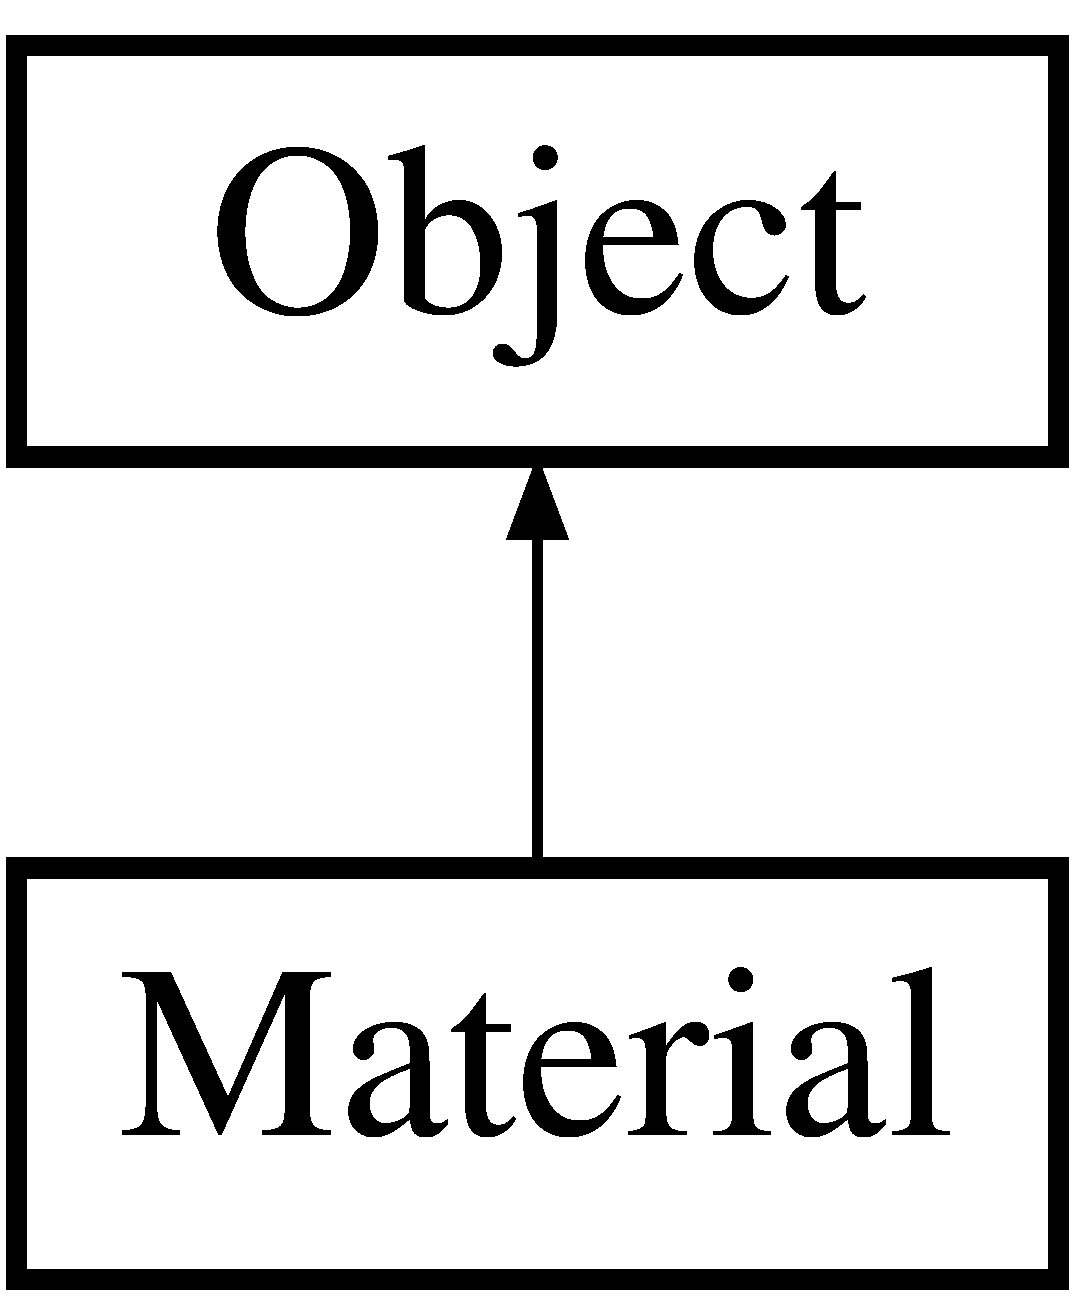
\includegraphics[height=2.000000cm]{class_material}
\end{center}
\end{figure}
\subsection*{Public Types}
\begin{DoxyCompactItemize}
\item 
enum \{ \\*
\hyperlink{class_material_a714370cb1e994ee8e526c1939530767fa237d6499dca28b1474ce39e09a90d492}{M\+A\+T\+\_\+\+W\+R\+AP} = 1, 
\hyperlink{class_material_a714370cb1e994ee8e526c1939530767fac6eac59fb07a11b02c2211a500275eec}{M\+A\+T\+\_\+\+W\+I\+RE} = 2, 
\hyperlink{class_material_a714370cb1e994ee8e526c1939530767fa5fcfa59c022ac6b23fb611ec8977abcf}{M\+A\+T\+\_\+\+Z\+A\+L\+W\+A\+YS} = 4, 
\hyperlink{class_material_a714370cb1e994ee8e526c1939530767fac095e1e2b52c4a352ece6c2d72f1c9dc}{M\+A\+T\+\_\+\+N\+O\+C\+U\+LL} = 8, 
\\*
\hyperlink{class_material_a714370cb1e994ee8e526c1939530767fabc06c866b4977529a1be0f5a01967c86}{M\+A\+T\+\_\+\+T\+R\+A\+NS} = 16
 \}
\end{DoxyCompactItemize}
\subsection*{Public Member Functions}
\begin{DoxyCompactItemize}
\item 
\hyperlink{class_material_a5c833e0bef6cb5afe3a697c3d2fd244a}{Material} (\hyperlink{class_texture}{Texture} $\ast$texture, char $\ast$vertex\+Shader\+Path=N\+U\+LL, char $\ast$pixel\+Shader\+Path=N\+U\+LL)
\begin{DoxyCompactList}\small\item\em Constructor. \end{DoxyCompactList}\item 
\hyperlink{class_material_a2c19452d71f54075df8f5405b03129f4}{$\sim$\+Material} ()
\begin{DoxyCompactList}\small\item\em Destructor. \end{DoxyCompactList}\item 
I\+D3\+D11\+Vertex\+Shader $\ast$ \hyperlink{class_material_ad0a3d883b957980fbc606bbbf9688d29}{Get\+Dx\+Vertex\+Shader} ()
\begin{DoxyCompactList}\small\item\em Getters. \end{DoxyCompactList}\item 
I\+D3\+D11\+Pixel\+Shader $\ast$ \hyperlink{class_material_a326382a866a4ad9f50c9d4a7e7b11f44}{Get\+Dx\+Pixel\+Shader} ()
\item 
I\+D3\+D11\+Input\+Layout $\ast$ \hyperlink{class_material_aab51c42d918132d3c50dea702cfb5d70}{Get\+Dx\+Input\+Layout} ()
\item 
I\+D3\+D11\+Sampler\+State $\ast$\& \hyperlink{class_material_a62903b3cc7607ee069f01ed31656a04d}{Get\+Dx\+Sampler\+State} ()
\item 
I\+D3\+D11\+Rasterizer\+State $\ast$ \hyperlink{class_material_a563a7e7b1561c84bc7e0a5535058d7a8}{Get\+Dx\+Rasterizer\+State} ()
\item 
I\+D3\+D11\+Depth\+Stencil\+State $\ast$ \hyperlink{class_material_adfed1977690dc11937f2fc2c181a61aa}{Get\+Dx\+Depth\+State} ()
\item 
I\+D3\+D11\+Blend\+State $\ast$ \hyperlink{class_material_a68d133ad75ced62ad4af090bd68bfe22}{Get\+Dx\+Blend\+State} ()
\item 
\hyperlink{class_texture}{Texture} $\ast$ \hyperlink{class_material_a84f3558e4be3b8ddc1c4b1e85d39d645}{Get\+Texture} ()
\item 
U\+I\+NT \& \hyperlink{class_material_afe7f86b971c00a0daa30839867539fb1}{Get\+Vertex\+Buffer\+Size} ()
\end{DoxyCompactItemize}
\subsection*{Protected Attributes}
\begin{DoxyCompactItemize}
\item 
I\+D3\+D11\+Vertex\+Shader $\ast$ \hyperlink{class_material_ada4d417d4e11a3151caba23c6d98ef18}{my\+Dx\+Vertex\+Shader}
\item 
I\+D3\+D11\+Pixel\+Shader $\ast$ \hyperlink{class_material_ab6f46cf000c8d88a47cf11b27ddaff46}{my\+Dx\+Pixel\+Shader}
\item 
I\+D3\+D11\+Input\+Layout $\ast$ \hyperlink{class_material_a72b8f75d4f289a8225c8f924964e4770}{my\+Dx\+Input\+Layout}
\item 
I\+D3\+D11\+Sampler\+State $\ast$ \hyperlink{class_material_a9825413b1ae64cbe5968b8678a68d0b9}{my\+Dx\+Sampler\+State}
\item 
I\+D3\+D11\+Rasterizer\+State $\ast$ \hyperlink{class_material_aa823a3d052a67d1ac95b54368984331e}{my\+Dx\+Rasterizer\+State}
\item 
I\+D3\+D11\+Depth\+Stencil\+State $\ast$ \hyperlink{class_material_a2992d32b4525b2f9e4b0005919ddf76e}{my\+Dx\+Depth\+State}
\item 
I\+D3\+D11\+Blend\+State $\ast$ \hyperlink{class_material_a7ca4cd5b86b5bb28a2223beb16927acb}{my\+Dx\+Blend\+State}
\item 
\hyperlink{class_texture}{Texture} $\ast$ \hyperlink{class_material_a8ff893b848c3392c63898b2951b6ec78}{my\+Texture}
\item 
U\+I\+NT \hyperlink{class_material_af0c062e2928f04c57056fe77f4f47f37}{my\+Vertex\+Buffer\+Size}
\end{DoxyCompactItemize}
\subsection*{Additional Inherited Members}


\subsection{Member Enumeration Documentation}
\subsubsection[{\texorpdfstring{anonymous enum}{anonymous enum}}]{\setlength{\rightskip}{0pt plus 5cm}anonymous enum}\hypertarget{class_material_a714370cb1e994ee8e526c1939530767f}{}\label{class_material_a714370cb1e994ee8e526c1939530767f}
\begin{Desc}
\item[Enumerator]\par
\begin{description}
\index{M\+A\+T\+\_\+\+W\+R\+AP@{M\+A\+T\+\_\+\+W\+R\+AP}!Material@{Material}}\index{Material@{Material}!M\+A\+T\+\_\+\+W\+R\+AP@{M\+A\+T\+\_\+\+W\+R\+AP}}\item[{\em 
M\+A\+T\+\_\+\+W\+R\+AP\hypertarget{class_material_a714370cb1e994ee8e526c1939530767fa237d6499dca28b1474ce39e09a90d492}{}\label{class_material_a714370cb1e994ee8e526c1939530767fa237d6499dca28b1474ce39e09a90d492}
}]\index{M\+A\+T\+\_\+\+W\+I\+RE@{M\+A\+T\+\_\+\+W\+I\+RE}!Material@{Material}}\index{Material@{Material}!M\+A\+T\+\_\+\+W\+I\+RE@{M\+A\+T\+\_\+\+W\+I\+RE}}\item[{\em 
M\+A\+T\+\_\+\+W\+I\+RE\hypertarget{class_material_a714370cb1e994ee8e526c1939530767fac6eac59fb07a11b02c2211a500275eec}{}\label{class_material_a714370cb1e994ee8e526c1939530767fac6eac59fb07a11b02c2211a500275eec}
}]\index{M\+A\+T\+\_\+\+Z\+A\+L\+W\+A\+YS@{M\+A\+T\+\_\+\+Z\+A\+L\+W\+A\+YS}!Material@{Material}}\index{Material@{Material}!M\+A\+T\+\_\+\+Z\+A\+L\+W\+A\+YS@{M\+A\+T\+\_\+\+Z\+A\+L\+W\+A\+YS}}\item[{\em 
M\+A\+T\+\_\+\+Z\+A\+L\+W\+A\+YS\hypertarget{class_material_a714370cb1e994ee8e526c1939530767fa5fcfa59c022ac6b23fb611ec8977abcf}{}\label{class_material_a714370cb1e994ee8e526c1939530767fa5fcfa59c022ac6b23fb611ec8977abcf}
}]\index{M\+A\+T\+\_\+\+N\+O\+C\+U\+LL@{M\+A\+T\+\_\+\+N\+O\+C\+U\+LL}!Material@{Material}}\index{Material@{Material}!M\+A\+T\+\_\+\+N\+O\+C\+U\+LL@{M\+A\+T\+\_\+\+N\+O\+C\+U\+LL}}\item[{\em 
M\+A\+T\+\_\+\+N\+O\+C\+U\+LL\hypertarget{class_material_a714370cb1e994ee8e526c1939530767fac095e1e2b52c4a352ece6c2d72f1c9dc}{}\label{class_material_a714370cb1e994ee8e526c1939530767fac095e1e2b52c4a352ece6c2d72f1c9dc}
}]\index{M\+A\+T\+\_\+\+T\+R\+A\+NS@{M\+A\+T\+\_\+\+T\+R\+A\+NS}!Material@{Material}}\index{Material@{Material}!M\+A\+T\+\_\+\+T\+R\+A\+NS@{M\+A\+T\+\_\+\+T\+R\+A\+NS}}\item[{\em 
M\+A\+T\+\_\+\+T\+R\+A\+NS\hypertarget{class_material_a714370cb1e994ee8e526c1939530767fabc06c866b4977529a1be0f5a01967c86}{}\label{class_material_a714370cb1e994ee8e526c1939530767fabc06c866b4977529a1be0f5a01967c86}
}]\end{description}
\end{Desc}


\subsection{Constructor \& Destructor Documentation}
\index{Material@{Material}!Material@{Material}}
\index{Material@{Material}!Material@{Material}}
\subsubsection[{\texorpdfstring{Material(\+Texture $\ast$texture, char $\ast$vertex\+Shader\+Path=\+N\+U\+L\+L, char $\ast$pixel\+Shader\+Path=\+N\+U\+L\+L)}{Material(Texture *texture, char *vertexShaderPath=NULL, char *pixelShaderPath=NULL)}}]{\setlength{\rightskip}{0pt plus 5cm}Material\+::\+Material (
\begin{DoxyParamCaption}
\item[{{\bf Texture} $\ast$}]{texture, }
\item[{char $\ast$}]{vertex\+Shader\+Path = {\ttfamily NULL}, }
\item[{char $\ast$}]{pixel\+Shader\+Path = {\ttfamily NULL}}
\end{DoxyParamCaption}
)}\hypertarget{class_material_a5c833e0bef6cb5afe3a697c3d2fd244a}{}\label{class_material_a5c833e0bef6cb5afe3a697c3d2fd244a}


Constructor. 

Constructor.

\begin{DoxyAuthor}{Author}
Katianie 
\end{DoxyAuthor}
\begin{DoxyDate}{Date}
7/4/2016
\end{DoxyDate}

\begin{DoxyParams}[1]{Parameters}
\mbox{\tt in}  & {\em texture} & If non-\/null, the texture. \\
\hline
\mbox{\tt in}  & {\em vertex\+Shader\+Path} & If non-\/null, full pathname of the vertex shader file. \\
\hline
\mbox{\tt in}  & {\em pixel\+Shader\+Path} & If non-\/null, full pathname of the pixel shader file. \\
\hline
\end{DoxyParams}
\index{Material@{Material}!````~Material@{$\sim$\+Material}}
\index{````~Material@{$\sim$\+Material}!Material@{Material}}
\subsubsection[{\texorpdfstring{$\sim$\+Material()}{~Material()}}]{\setlength{\rightskip}{0pt plus 5cm}Material\+::$\sim$\+Material (
\begin{DoxyParamCaption}
{}
\end{DoxyParamCaption}
)}\hypertarget{class_material_a2c19452d71f54075df8f5405b03129f4}{}\label{class_material_a2c19452d71f54075df8f5405b03129f4}


Destructor. 

Destructor.

\begin{DoxyAuthor}{Author}
Katianie 
\end{DoxyAuthor}
\begin{DoxyDate}{Date}
7/4/2016 
\end{DoxyDate}


\subsection{Member Function Documentation}
\index{Material@{Material}!Get\+Dx\+Blend\+State@{Get\+Dx\+Blend\+State}}
\index{Get\+Dx\+Blend\+State@{Get\+Dx\+Blend\+State}!Material@{Material}}
\subsubsection[{\texorpdfstring{Get\+Dx\+Blend\+State()}{GetDxBlendState()}}]{\setlength{\rightskip}{0pt plus 5cm}I\+D3\+D11\+Blend\+State $\ast$ Material\+::\+Get\+Dx\+Blend\+State (
\begin{DoxyParamCaption}
{}
\end{DoxyParamCaption}
)}\hypertarget{class_material_a68d133ad75ced62ad4af090bd68bfe22}{}\label{class_material_a68d133ad75ced62ad4af090bd68bfe22}
Gets the DX Blend State.

\begin{DoxyAuthor}{Author}
Katianie 
\end{DoxyAuthor}
\begin{DoxyDate}{Date}
7/4/2016
\end{DoxyDate}
\begin{DoxyReturn}{Returns}
The DX Blend State. 
\end{DoxyReturn}
\index{Material@{Material}!Get\+Dx\+Depth\+State@{Get\+Dx\+Depth\+State}}
\index{Get\+Dx\+Depth\+State@{Get\+Dx\+Depth\+State}!Material@{Material}}
\subsubsection[{\texorpdfstring{Get\+Dx\+Depth\+State()}{GetDxDepthState()}}]{\setlength{\rightskip}{0pt plus 5cm}I\+D3\+D11\+Depth\+Stencil\+State $\ast$ Material\+::\+Get\+Dx\+Depth\+State (
\begin{DoxyParamCaption}
{}
\end{DoxyParamCaption}
)}\hypertarget{class_material_adfed1977690dc11937f2fc2c181a61aa}{}\label{class_material_adfed1977690dc11937f2fc2c181a61aa}
Gets the DX Depth State.

\begin{DoxyAuthor}{Author}
Katianie 
\end{DoxyAuthor}
\begin{DoxyDate}{Date}
7/4/2016
\end{DoxyDate}
\begin{DoxyReturn}{Returns}
The DX Depth State. 
\end{DoxyReturn}
\index{Material@{Material}!Get\+Dx\+Input\+Layout@{Get\+Dx\+Input\+Layout}}
\index{Get\+Dx\+Input\+Layout@{Get\+Dx\+Input\+Layout}!Material@{Material}}
\subsubsection[{\texorpdfstring{Get\+Dx\+Input\+Layout()}{GetDxInputLayout()}}]{\setlength{\rightskip}{0pt plus 5cm}I\+D3\+D11\+Input\+Layout $\ast$ Material\+::\+Get\+Dx\+Input\+Layout (
\begin{DoxyParamCaption}
{}
\end{DoxyParamCaption}
)}\hypertarget{class_material_aab51c42d918132d3c50dea702cfb5d70}{}\label{class_material_aab51c42d918132d3c50dea702cfb5d70}
Gets the DX Input Layout.

\begin{DoxyAuthor}{Author}
Katianie 
\end{DoxyAuthor}
\begin{DoxyDate}{Date}
7/4/2016
\end{DoxyDate}
\begin{DoxyReturn}{Returns}
The DX Input Layout. 
\end{DoxyReturn}
\index{Material@{Material}!Get\+Dx\+Pixel\+Shader@{Get\+Dx\+Pixel\+Shader}}
\index{Get\+Dx\+Pixel\+Shader@{Get\+Dx\+Pixel\+Shader}!Material@{Material}}
\subsubsection[{\texorpdfstring{Get\+Dx\+Pixel\+Shader()}{GetDxPixelShader()}}]{\setlength{\rightskip}{0pt plus 5cm}I\+D3\+D11\+Pixel\+Shader $\ast$ Material\+::\+Get\+Dx\+Pixel\+Shader (
\begin{DoxyParamCaption}
{}
\end{DoxyParamCaption}
)}\hypertarget{class_material_a326382a866a4ad9f50c9d4a7e7b11f44}{}\label{class_material_a326382a866a4ad9f50c9d4a7e7b11f44}
Gets DX Pixel Shader.

\begin{DoxyAuthor}{Author}
Katianie 
\end{DoxyAuthor}
\begin{DoxyDate}{Date}
7/4/2016
\end{DoxyDate}
\begin{DoxyReturn}{Returns}
The DX Pixel Shader. 
\end{DoxyReturn}
\index{Material@{Material}!Get\+Dx\+Rasterizer\+State@{Get\+Dx\+Rasterizer\+State}}
\index{Get\+Dx\+Rasterizer\+State@{Get\+Dx\+Rasterizer\+State}!Material@{Material}}
\subsubsection[{\texorpdfstring{Get\+Dx\+Rasterizer\+State()}{GetDxRasterizerState()}}]{\setlength{\rightskip}{0pt plus 5cm}I\+D3\+D11\+Rasterizer\+State $\ast$ Material\+::\+Get\+Dx\+Rasterizer\+State (
\begin{DoxyParamCaption}
{}
\end{DoxyParamCaption}
)}\hypertarget{class_material_a563a7e7b1561c84bc7e0a5535058d7a8}{}\label{class_material_a563a7e7b1561c84bc7e0a5535058d7a8}
Gets the DX Rasterizer State.

\begin{DoxyAuthor}{Author}
Katianie 
\end{DoxyAuthor}
\begin{DoxyDate}{Date}
7/4/2016
\end{DoxyDate}
\begin{DoxyReturn}{Returns}
The DX Rasterizer State. 
\end{DoxyReturn}
\index{Material@{Material}!Get\+Dx\+Sampler\+State@{Get\+Dx\+Sampler\+State}}
\index{Get\+Dx\+Sampler\+State@{Get\+Dx\+Sampler\+State}!Material@{Material}}
\subsubsection[{\texorpdfstring{Get\+Dx\+Sampler\+State()}{GetDxSamplerState()}}]{\setlength{\rightskip}{0pt plus 5cm}I\+D3\+D11\+Sampler\+State $\ast$\& Material\+::\+Get\+Dx\+Sampler\+State (
\begin{DoxyParamCaption}
{}
\end{DoxyParamCaption}
)}\hypertarget{class_material_a62903b3cc7607ee069f01ed31656a04d}{}\label{class_material_a62903b3cc7607ee069f01ed31656a04d}
Gets the DX Sampler State.

\begin{DoxyAuthor}{Author}
Katianie 
\end{DoxyAuthor}
\begin{DoxyDate}{Date}
7/4/2016
\end{DoxyDate}
\begin{DoxyReturn}{Returns}
The DX Sampler State. 
\end{DoxyReturn}
\index{Material@{Material}!Get\+Dx\+Vertex\+Shader@{Get\+Dx\+Vertex\+Shader}}
\index{Get\+Dx\+Vertex\+Shader@{Get\+Dx\+Vertex\+Shader}!Material@{Material}}
\subsubsection[{\texorpdfstring{Get\+Dx\+Vertex\+Shader()}{GetDxVertexShader()}}]{\setlength{\rightskip}{0pt plus 5cm}I\+D3\+D11\+Vertex\+Shader $\ast$ Material\+::\+Get\+Dx\+Vertex\+Shader (
\begin{DoxyParamCaption}
{}
\end{DoxyParamCaption}
)}\hypertarget{class_material_ad0a3d883b957980fbc606bbbf9688d29}{}\label{class_material_ad0a3d883b957980fbc606bbbf9688d29}


Getters. 

Gets the DX \hyperlink{class_vertex}{Vertex} Shader.

\begin{DoxyAuthor}{Author}
Katianie 
\end{DoxyAuthor}
\begin{DoxyDate}{Date}
7/4/2016
\end{DoxyDate}
\begin{DoxyReturn}{Returns}
The DX \hyperlink{class_vertex}{Vertex} Shader. 
\end{DoxyReturn}
\index{Material@{Material}!Get\+Texture@{Get\+Texture}}
\index{Get\+Texture@{Get\+Texture}!Material@{Material}}
\subsubsection[{\texorpdfstring{Get\+Texture()}{GetTexture()}}]{\setlength{\rightskip}{0pt plus 5cm}{\bf Texture} $\ast$ Material\+::\+Get\+Texture (
\begin{DoxyParamCaption}
{}
\end{DoxyParamCaption}
)}\hypertarget{class_material_a84f3558e4be3b8ddc1c4b1e85d39d645}{}\label{class_material_a84f3558e4be3b8ddc1c4b1e85d39d645}
Gets the \hyperlink{class_texture}{Texture}.

\begin{DoxyAuthor}{Author}
Katianie 
\end{DoxyAuthor}
\begin{DoxyDate}{Date}
7/4/2016
\end{DoxyDate}
\begin{DoxyReturn}{Returns}
The \hyperlink{class_texture}{Texture}. 
\end{DoxyReturn}
\index{Material@{Material}!Get\+Vertex\+Buffer\+Size@{Get\+Vertex\+Buffer\+Size}}
\index{Get\+Vertex\+Buffer\+Size@{Get\+Vertex\+Buffer\+Size}!Material@{Material}}
\subsubsection[{\texorpdfstring{Get\+Vertex\+Buffer\+Size()}{GetVertexBufferSize()}}]{\setlength{\rightskip}{0pt plus 5cm}U\+I\+NT \& Material\+::\+Get\+Vertex\+Buffer\+Size (
\begin{DoxyParamCaption}
{}
\end{DoxyParamCaption}
)}\hypertarget{class_material_afe7f86b971c00a0daa30839867539fb1}{}\label{class_material_afe7f86b971c00a0daa30839867539fb1}
Gets the \hyperlink{class_vertex}{Vertex} Buffer size.

\begin{DoxyAuthor}{Author}
Katianie 
\end{DoxyAuthor}
\begin{DoxyDate}{Date}
7/4/2016
\end{DoxyDate}
\begin{DoxyReturn}{Returns}
The \hyperlink{class_vertex}{Vertex} Buffer size. 
\end{DoxyReturn}


\subsection{Member Data Documentation}
\index{Material@{Material}!my\+Dx\+Blend\+State@{my\+Dx\+Blend\+State}}
\index{my\+Dx\+Blend\+State@{my\+Dx\+Blend\+State}!Material@{Material}}
\subsubsection[{\texorpdfstring{my\+Dx\+Blend\+State}{myDxBlendState}}]{\setlength{\rightskip}{0pt plus 5cm}I\+D3\+D11\+Blend\+State$\ast$ Material\+::my\+Dx\+Blend\+State\hspace{0.3cm}{\ttfamily [protected]}}\hypertarget{class_material_a7ca4cd5b86b5bb28a2223beb16927acb}{}\label{class_material_a7ca4cd5b86b5bb28a2223beb16927acb}
\index{Material@{Material}!my\+Dx\+Depth\+State@{my\+Dx\+Depth\+State}}
\index{my\+Dx\+Depth\+State@{my\+Dx\+Depth\+State}!Material@{Material}}
\subsubsection[{\texorpdfstring{my\+Dx\+Depth\+State}{myDxDepthState}}]{\setlength{\rightskip}{0pt plus 5cm}I\+D3\+D11\+Depth\+Stencil\+State$\ast$ Material\+::my\+Dx\+Depth\+State\hspace{0.3cm}{\ttfamily [protected]}}\hypertarget{class_material_a2992d32b4525b2f9e4b0005919ddf76e}{}\label{class_material_a2992d32b4525b2f9e4b0005919ddf76e}
\index{Material@{Material}!my\+Dx\+Input\+Layout@{my\+Dx\+Input\+Layout}}
\index{my\+Dx\+Input\+Layout@{my\+Dx\+Input\+Layout}!Material@{Material}}
\subsubsection[{\texorpdfstring{my\+Dx\+Input\+Layout}{myDxInputLayout}}]{\setlength{\rightskip}{0pt plus 5cm}I\+D3\+D11\+Input\+Layout$\ast$ Material\+::my\+Dx\+Input\+Layout\hspace{0.3cm}{\ttfamily [protected]}}\hypertarget{class_material_a72b8f75d4f289a8225c8f924964e4770}{}\label{class_material_a72b8f75d4f289a8225c8f924964e4770}
\index{Material@{Material}!my\+Dx\+Pixel\+Shader@{my\+Dx\+Pixel\+Shader}}
\index{my\+Dx\+Pixel\+Shader@{my\+Dx\+Pixel\+Shader}!Material@{Material}}
\subsubsection[{\texorpdfstring{my\+Dx\+Pixel\+Shader}{myDxPixelShader}}]{\setlength{\rightskip}{0pt plus 5cm}I\+D3\+D11\+Pixel\+Shader$\ast$ Material\+::my\+Dx\+Pixel\+Shader\hspace{0.3cm}{\ttfamily [protected]}}\hypertarget{class_material_ab6f46cf000c8d88a47cf11b27ddaff46}{}\label{class_material_ab6f46cf000c8d88a47cf11b27ddaff46}
\index{Material@{Material}!my\+Dx\+Rasterizer\+State@{my\+Dx\+Rasterizer\+State}}
\index{my\+Dx\+Rasterizer\+State@{my\+Dx\+Rasterizer\+State}!Material@{Material}}
\subsubsection[{\texorpdfstring{my\+Dx\+Rasterizer\+State}{myDxRasterizerState}}]{\setlength{\rightskip}{0pt plus 5cm}I\+D3\+D11\+Rasterizer\+State$\ast$ Material\+::my\+Dx\+Rasterizer\+State\hspace{0.3cm}{\ttfamily [protected]}}\hypertarget{class_material_aa823a3d052a67d1ac95b54368984331e}{}\label{class_material_aa823a3d052a67d1ac95b54368984331e}
\index{Material@{Material}!my\+Dx\+Sampler\+State@{my\+Dx\+Sampler\+State}}
\index{my\+Dx\+Sampler\+State@{my\+Dx\+Sampler\+State}!Material@{Material}}
\subsubsection[{\texorpdfstring{my\+Dx\+Sampler\+State}{myDxSamplerState}}]{\setlength{\rightskip}{0pt plus 5cm}I\+D3\+D11\+Sampler\+State$\ast$ Material\+::my\+Dx\+Sampler\+State\hspace{0.3cm}{\ttfamily [protected]}}\hypertarget{class_material_a9825413b1ae64cbe5968b8678a68d0b9}{}\label{class_material_a9825413b1ae64cbe5968b8678a68d0b9}
\index{Material@{Material}!my\+Dx\+Vertex\+Shader@{my\+Dx\+Vertex\+Shader}}
\index{my\+Dx\+Vertex\+Shader@{my\+Dx\+Vertex\+Shader}!Material@{Material}}
\subsubsection[{\texorpdfstring{my\+Dx\+Vertex\+Shader}{myDxVertexShader}}]{\setlength{\rightskip}{0pt plus 5cm}I\+D3\+D11\+Vertex\+Shader$\ast$ Material\+::my\+Dx\+Vertex\+Shader\hspace{0.3cm}{\ttfamily [protected]}}\hypertarget{class_material_ada4d417d4e11a3151caba23c6d98ef18}{}\label{class_material_ada4d417d4e11a3151caba23c6d98ef18}
\index{Material@{Material}!my\+Texture@{my\+Texture}}
\index{my\+Texture@{my\+Texture}!Material@{Material}}
\subsubsection[{\texorpdfstring{my\+Texture}{myTexture}}]{\setlength{\rightskip}{0pt plus 5cm}{\bf Texture}$\ast$ Material\+::my\+Texture\hspace{0.3cm}{\ttfamily [protected]}}\hypertarget{class_material_a8ff893b848c3392c63898b2951b6ec78}{}\label{class_material_a8ff893b848c3392c63898b2951b6ec78}
\index{Material@{Material}!my\+Vertex\+Buffer\+Size@{my\+Vertex\+Buffer\+Size}}
\index{my\+Vertex\+Buffer\+Size@{my\+Vertex\+Buffer\+Size}!Material@{Material}}
\subsubsection[{\texorpdfstring{my\+Vertex\+Buffer\+Size}{myVertexBufferSize}}]{\setlength{\rightskip}{0pt plus 5cm}U\+I\+NT Material\+::my\+Vertex\+Buffer\+Size\hspace{0.3cm}{\ttfamily [protected]}}\hypertarget{class_material_af0c062e2928f04c57056fe77f4f47f37}{}\label{class_material_af0c062e2928f04c57056fe77f4f47f37}


The documentation for this class was generated from the following files\+:\begin{DoxyCompactItemize}
\item 
Samples/\+Oculus\+Room\+Tiny\+\_\+\+Advanced/\+Common/\+Headers/\hyperlink{_material_8h}{Material.\+h}\item 
Samples/\+Oculus\+Room\+Tiny\+\_\+\+Advanced/\+Common/\+Implementations/\hyperlink{_material_8cpp}{Material.\+cpp}\end{DoxyCompactItemize}

\hypertarget{class_model}{}\section{Model Class Reference}
\label{class_model}\index{Model@{Model}}


{\ttfamily \#include $<$Model.\+h$>$}

Inheritance diagram for Model\+:\begin{figure}[H]
\begin{center}
\leavevmode
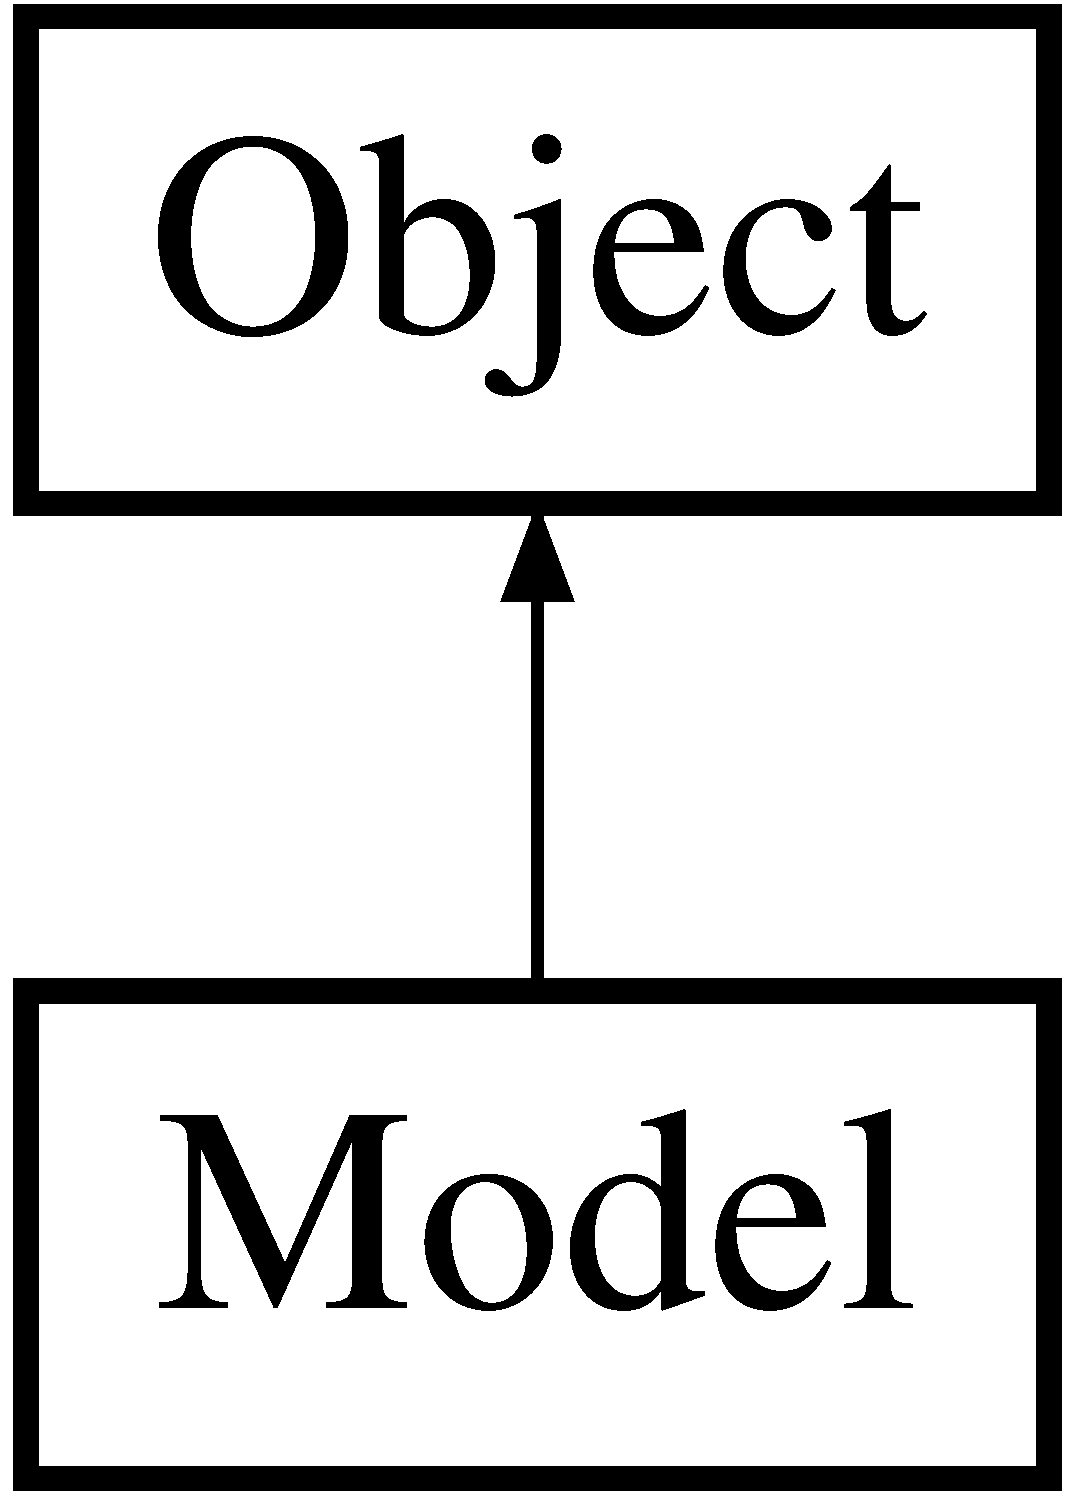
\includegraphics[height=2.000000cm]{class_model}
\end{center}
\end{figure}
\subsection*{Public Member Functions}
\begin{DoxyCompactItemize}
\item 
\hyperlink{class_model_ae3b375de5f6df4faf74a95d64748e048}{Model} ()
\begin{DoxyCompactList}\small\item\em Constructors. \end{DoxyCompactList}\item 
\hyperlink{class_model_a5b3fa50a40180b5ef48ba593f9b39b9e}{Model} (int panoramic\+Type, \hyperlink{class_triangle_set}{Triangle\+Set} $\ast$triangle\+Set, X\+M\+F\+L\+O\+A\+T3 model\+Position, X\+M\+F\+L\+O\+A\+T4 model\+Rotation, \hyperlink{class_material}{Material} $\ast$model\+Material)
\item 
void \hyperlink{class_model_ade8ba725d673d2ff8f375e86201253cc}{Init} (int panoramic\+Type, \hyperlink{class_triangle_set}{Triangle\+Set} $\ast$triangle\+Set)
\item 
\hyperlink{class_model_ad6ebd2062a0b823db841a0b88baac4c0}{$\sim$\+Model} ()
\begin{DoxyCompactList}\small\item\em Destructor. \end{DoxyCompactList}\item 
void \hyperlink{class_model_a10bcb6448b90831453b9069f3979ed45}{Render} (X\+M\+M\+A\+T\+R\+IX $\ast$proj\+View, float red, float green, float blue, float alpha)
\begin{DoxyCompactList}\small\item\em Functions. \end{DoxyCompactList}\item 
\hyperlink{class_data_buffer}{Data\+Buffer} $\ast$ \hyperlink{class_model_acfc34c5ad56cb176e29e65d32312379c}{Get\+Index\+Buffer} ()
\begin{DoxyCompactList}\small\item\em Getters. \end{DoxyCompactList}\item 
\hyperlink{class_material}{Material} $\ast$ \hyperlink{class_model_a0294c00f16232d82105e362dab9ef1c0}{Get\+Material} ()
\item 
int \hyperlink{class_model_a57f8b0739bc9e9b1792daedb28ebb51d}{Get\+Num\+Indices} ()
\item 
X\+M\+F\+L\+O\+A\+T3 \hyperlink{class_model_a6b7189ab637042cb8d316d8f6bf87ad3}{Get\+Position} ()
\item 
X\+M\+F\+L\+O\+A\+T4 \hyperlink{class_model_ae7118e3d1858d7a0e70a3556d7f5193a}{Get\+Rotation} ()
\item 
\hyperlink{class_data_buffer}{Data\+Buffer} $\ast$ \hyperlink{class_model_af036bab5ce7d59f78b421b499fbd7504}{Get\+Vertex\+Buffer} ()
\item 
void \hyperlink{class_model_adc03916b48d42a1321510687e0b5d934}{Set\+Position} (X\+M\+F\+L\+O\+A\+T3 pos)
\begin{DoxyCompactList}\small\item\em Setters. \end{DoxyCompactList}\end{DoxyCompactItemize}
\subsection*{Protected Attributes}
\begin{DoxyCompactItemize}
\item 
X\+M\+F\+L\+O\+A\+T3 \hyperlink{class_model_a5fb219d082bc479627d5e1e66b33fe63}{my\+Position}
\item 
X\+M\+F\+L\+O\+A\+T4 \hyperlink{class_model_a4a374cf09dc49e48dfa106f60bcb3d97}{my\+First\+Position}
\item 
X\+M\+F\+L\+O\+A\+T4 \hyperlink{class_model_abd379baa73dacba16b7ed238982c1a06}{my\+Rotation}
\item 
\hyperlink{class_material}{Material} $\ast$ \hyperlink{class_model_a6b749b5e9c3eb936b380a85b6800cce6}{my\+Material}
\item 
\hyperlink{class_data_buffer}{Data\+Buffer} $\ast$ \hyperlink{class_model_a64e673cb0b3c36e014606c73138486de}{my\+Vertex\+Buffer}
\item 
\hyperlink{class_data_buffer}{Data\+Buffer} $\ast$ \hyperlink{class_model_a920be5d05f546b78e696adfd481da15c}{my\+Index\+Buffer}
\item 
int \hyperlink{class_model_ab0a5ce9fd0d759718453417e8c31b902}{my\+Num\+Indices}
\end{DoxyCompactItemize}
\subsection*{Additional Inherited Members}


\subsection{Constructor \& Destructor Documentation}
\index{Model@{Model}!Model@{Model}}
\index{Model@{Model}!Model@{Model}}
\subsubsection[{\texorpdfstring{Model()}{Model()}}]{\setlength{\rightskip}{0pt plus 5cm}Model\+::\+Model (
\begin{DoxyParamCaption}
{}
\end{DoxyParamCaption}
)}\hypertarget{class_model_ae3b375de5f6df4faf74a95d64748e048}{}\label{class_model_ae3b375de5f6df4faf74a95d64748e048}


Constructors. 

Default Constructor.

\begin{DoxyAuthor}{Author}
Katianie 
\end{DoxyAuthor}
\begin{DoxyDate}{Date}
7/4/2016 
\end{DoxyDate}
\index{Model@{Model}!Model@{Model}}
\index{Model@{Model}!Model@{Model}}
\subsubsection[{\texorpdfstring{Model(int panoramic\+Type, Triangle\+Set $\ast$triangle\+Set, X\+M\+F\+L\+O\+A\+T3 model\+Position, X\+M\+F\+L\+O\+A\+T4 model\+Rotation, Material $\ast$model\+Material)}{Model(int panoramicType, TriangleSet *triangleSet, XMFLOAT3 modelPosition, XMFLOAT4 modelRotation, Material *modelMaterial)}}]{\setlength{\rightskip}{0pt plus 5cm}Model\+::\+Model (
\begin{DoxyParamCaption}
\item[{int}]{panoramic\+Type, }
\item[{{\bf Triangle\+Set} $\ast$}]{triangle\+Set, }
\item[{X\+M\+F\+L\+O\+A\+T3}]{model\+Position, }
\item[{X\+M\+F\+L\+O\+A\+T4}]{model\+Rotation, }
\item[{{\bf Material} $\ast$}]{model\+Material}
\end{DoxyParamCaption}
)}\hypertarget{class_model_a5b3fa50a40180b5ef48ba593f9b39b9e}{}\label{class_model_a5b3fa50a40180b5ef48ba593f9b39b9e}
Parameterized Constructor, also calls \hyperlink{class_model_ade8ba725d673d2ff8f375e86201253cc}{Init()}.

\begin{DoxyAuthor}{Author}
Katianie 
\end{DoxyAuthor}
\begin{DoxyDate}{Date}
7/4/2016
\end{DoxyDate}

\begin{DoxyParams}[1]{Parameters}
 & {\em panoramic\+Type} & Type of the panoramic (180, 270, 360, or 999 for photosphere). \\
\hline
\mbox{\tt in,out}  & {\em triangle\+Set} & If non-\/null, set the triangle belongs to. \\
\hline
 & {\em model\+Position} & The model position. \\
\hline
 & {\em model\+Rotation} & The model rotation. \\
\hline
\mbox{\tt in,out}  & {\em model\+Material} & If non-\/null, the model material. \\
\hline
\end{DoxyParams}
\index{Model@{Model}!````~Model@{$\sim$\+Model}}
\index{````~Model@{$\sim$\+Model}!Model@{Model}}
\subsubsection[{\texorpdfstring{$\sim$\+Model()}{~Model()}}]{\setlength{\rightskip}{0pt plus 5cm}Model\+::$\sim$\+Model (
\begin{DoxyParamCaption}
{}
\end{DoxyParamCaption}
)}\hypertarget{class_model_ad6ebd2062a0b823db841a0b88baac4c0}{}\label{class_model_ad6ebd2062a0b823db841a0b88baac4c0}


Destructor. 

Destructor, Deletes the model and cleans up.

\begin{DoxyAuthor}{Author}
Katianie 
\end{DoxyAuthor}
\begin{DoxyDate}{Date}
7/4/2016 
\end{DoxyDate}


\subsection{Member Function Documentation}
\index{Model@{Model}!Get\+Index\+Buffer@{Get\+Index\+Buffer}}
\index{Get\+Index\+Buffer@{Get\+Index\+Buffer}!Model@{Model}}
\subsubsection[{\texorpdfstring{Get\+Index\+Buffer()}{GetIndexBuffer()}}]{\setlength{\rightskip}{0pt plus 5cm}{\bf Data\+Buffer} $\ast$ Model\+::\+Get\+Index\+Buffer (
\begin{DoxyParamCaption}
{}
\end{DoxyParamCaption}
)}\hypertarget{class_model_acfc34c5ad56cb176e29e65d32312379c}{}\label{class_model_acfc34c5ad56cb176e29e65d32312379c}


Getters. 

Gets the index buffer.

\begin{DoxyAuthor}{Author}
Katianie 
\end{DoxyAuthor}
\begin{DoxyDate}{Date}
7/4/2016
\end{DoxyDate}
\begin{DoxyReturn}{Returns}
The index buffer. 
\end{DoxyReturn}
\index{Model@{Model}!Get\+Material@{Get\+Material}}
\index{Get\+Material@{Get\+Material}!Model@{Model}}
\subsubsection[{\texorpdfstring{Get\+Material()}{GetMaterial()}}]{\setlength{\rightskip}{0pt plus 5cm}{\bf Material} $\ast$ Model\+::\+Get\+Material (
\begin{DoxyParamCaption}
{}
\end{DoxyParamCaption}
)}\hypertarget{class_model_a0294c00f16232d82105e362dab9ef1c0}{}\label{class_model_a0294c00f16232d82105e362dab9ef1c0}
Gets the material.

\begin{DoxyAuthor}{Author}
Katianie 
\end{DoxyAuthor}
\begin{DoxyDate}{Date}
7/4/2016
\end{DoxyDate}
\begin{DoxyReturn}{Returns}
The material. 
\end{DoxyReturn}
\index{Model@{Model}!Get\+Num\+Indices@{Get\+Num\+Indices}}
\index{Get\+Num\+Indices@{Get\+Num\+Indices}!Model@{Model}}
\subsubsection[{\texorpdfstring{Get\+Num\+Indices()}{GetNumIndices()}}]{\setlength{\rightskip}{0pt plus 5cm}int Model\+::\+Get\+Num\+Indices (
\begin{DoxyParamCaption}
{}
\end{DoxyParamCaption}
)}\hypertarget{class_model_a57f8b0739bc9e9b1792daedb28ebb51d}{}\label{class_model_a57f8b0739bc9e9b1792daedb28ebb51d}
Gets the number indices.

\begin{DoxyAuthor}{Author}
Katianie 
\end{DoxyAuthor}
\begin{DoxyDate}{Date}
7/4/2016
\end{DoxyDate}
\begin{DoxyReturn}{Returns}
The number indices. 
\end{DoxyReturn}
\index{Model@{Model}!Get\+Position@{Get\+Position}}
\index{Get\+Position@{Get\+Position}!Model@{Model}}
\subsubsection[{\texorpdfstring{Get\+Position()}{GetPosition()}}]{\setlength{\rightskip}{0pt plus 5cm}X\+M\+F\+L\+O\+A\+T3 Model\+::\+Get\+Position (
\begin{DoxyParamCaption}
{}
\end{DoxyParamCaption}
)}\hypertarget{class_model_a6b7189ab637042cb8d316d8f6bf87ad3}{}\label{class_model_a6b7189ab637042cb8d316d8f6bf87ad3}
Gets the position of the \hyperlink{class_model}{Model}.

\begin{DoxyAuthor}{Author}
Katianie 
\end{DoxyAuthor}
\begin{DoxyDate}{Date}
7/4/2016
\end{DoxyDate}
\begin{DoxyReturn}{Returns}
The position. 
\end{DoxyReturn}
\index{Model@{Model}!Get\+Rotation@{Get\+Rotation}}
\index{Get\+Rotation@{Get\+Rotation}!Model@{Model}}
\subsubsection[{\texorpdfstring{Get\+Rotation()}{GetRotation()}}]{\setlength{\rightskip}{0pt plus 5cm}X\+M\+F\+L\+O\+A\+T4 Model\+::\+Get\+Rotation (
\begin{DoxyParamCaption}
{}
\end{DoxyParamCaption}
)}\hypertarget{class_model_ae7118e3d1858d7a0e70a3556d7f5193a}{}\label{class_model_ae7118e3d1858d7a0e70a3556d7f5193a}
Gets the rotation vector of the model. The x,y,z components are the axis and the w component is the angle of rotation in degrees.

\begin{DoxyAuthor}{Author}
Katianie 
\end{DoxyAuthor}
\begin{DoxyDate}{Date}
7/4/2016
\end{DoxyDate}
\begin{DoxyReturn}{Returns}
The rotation vector and angle. 
\end{DoxyReturn}
\index{Model@{Model}!Get\+Vertex\+Buffer@{Get\+Vertex\+Buffer}}
\index{Get\+Vertex\+Buffer@{Get\+Vertex\+Buffer}!Model@{Model}}
\subsubsection[{\texorpdfstring{Get\+Vertex\+Buffer()}{GetVertexBuffer()}}]{\setlength{\rightskip}{0pt plus 5cm}{\bf Data\+Buffer} $\ast$ Model\+::\+Get\+Vertex\+Buffer (
\begin{DoxyParamCaption}
{}
\end{DoxyParamCaption}
)}\hypertarget{class_model_af036bab5ce7d59f78b421b499fbd7504}{}\label{class_model_af036bab5ce7d59f78b421b499fbd7504}
Gets the vertex buffer.

\begin{DoxyAuthor}{Author}
Katianie 
\end{DoxyAuthor}
\begin{DoxyDate}{Date}
7/4/2016
\end{DoxyDate}
\begin{DoxyReturn}{Returns}
The vertex buffer. 
\end{DoxyReturn}
\index{Model@{Model}!Init@{Init}}
\index{Init@{Init}!Model@{Model}}
\subsubsection[{\texorpdfstring{Init(int panoramic\+Type, Triangle\+Set $\ast$triangle\+Set)}{Init(int panoramicType, TriangleSet *triangleSet)}}]{\setlength{\rightskip}{0pt plus 5cm}void Model\+::\+Init (
\begin{DoxyParamCaption}
\item[{int}]{panoramic\+Type, }
\item[{{\bf Triangle\+Set} $\ast$}]{triangle\+Set}
\end{DoxyParamCaption}
)}\hypertarget{class_model_ade8ba725d673d2ff8f375e86201253cc}{}\label{class_model_ade8ba725d673d2ff8f375e86201253cc}
Initializes the model by taking in the geometry and the type of panoramic (180, 270, 360, and 999 for photosphere).

\begin{DoxyAuthor}{Author}
Katianie 
\end{DoxyAuthor}
\begin{DoxyDate}{Date}
7/4/2016
\end{DoxyDate}

\begin{DoxyParams}[1]{Parameters}
 & {\em panoramic\+Type} & Type of the panoramic. \\
\hline
\mbox{\tt in,out}  & {\em triangle\+Set} & If non-\/null, set the triangle belongs to. \\
\hline
\end{DoxyParams}
\index{Model@{Model}!Render@{Render}}
\index{Render@{Render}!Model@{Model}}
\subsubsection[{\texorpdfstring{Render(\+X\+M\+M\+A\+T\+R\+I\+X $\ast$proj\+View, float red, float green, float blue, float alpha)}{Render(XMMATRIX *projView, float red, float green, float blue, float alpha)}}]{\setlength{\rightskip}{0pt plus 5cm}void Model\+::\+Render (
\begin{DoxyParamCaption}
\item[{X\+M\+M\+A\+T\+R\+IX $\ast$}]{proj\+View, }
\item[{float}]{red, }
\item[{float}]{green, }
\item[{float}]{blue, }
\item[{float}]{alpha}
\end{DoxyParamCaption}
)}\hypertarget{class_model_a10bcb6448b90831453b9069f3979ed45}{}\label{class_model_a10bcb6448b90831453b9069f3979ed45}


Functions. 

Primary render function, renders the model (geometry, material, and shader data).

\begin{DoxyAuthor}{Author}
Katianie 
\end{DoxyAuthor}
\begin{DoxyDate}{Date}
7/4/2016
\end{DoxyDate}

\begin{DoxyParams}[1]{Parameters}
\mbox{\tt in}  & {\em proj\+View} & The \hyperlink{class_model}{Model} View Projection matrix. \\
\hline
 & {\em red} & The red color value for the current pixel. \\
\hline
 & {\em green} & The green color value for the current pixel. \\
\hline
 & {\em blue} & The blue color value for the current pixel. \\
\hline
 & {\em alpha} & The alpha color value for the current pixel. \\
\hline
\end{DoxyParams}
\index{Model@{Model}!Set\+Position@{Set\+Position}}
\index{Set\+Position@{Set\+Position}!Model@{Model}}
\subsubsection[{\texorpdfstring{Set\+Position(\+X\+M\+F\+L\+O\+A\+T3 pos)}{SetPosition(XMFLOAT3 pos)}}]{\setlength{\rightskip}{0pt plus 5cm}void Model\+::\+Set\+Position (
\begin{DoxyParamCaption}
\item[{X\+M\+F\+L\+O\+A\+T3}]{pos}
\end{DoxyParamCaption}
)}\hypertarget{class_model_adc03916b48d42a1321510687e0b5d934}{}\label{class_model_adc03916b48d42a1321510687e0b5d934}


Setters. 

Sets the position.

\begin{DoxyAuthor}{Author}
Katianie 
\end{DoxyAuthor}
\begin{DoxyDate}{Date}
7/4/2016
\end{DoxyDate}

\begin{DoxyParams}{Parameters}
{\em pos} & The new position. \\
\hline
\end{DoxyParams}


\subsection{Member Data Documentation}
\index{Model@{Model}!my\+First\+Position@{my\+First\+Position}}
\index{my\+First\+Position@{my\+First\+Position}!Model@{Model}}
\subsubsection[{\texorpdfstring{my\+First\+Position}{myFirstPosition}}]{\setlength{\rightskip}{0pt plus 5cm}X\+M\+F\+L\+O\+A\+T4 Model\+::my\+First\+Position\hspace{0.3cm}{\ttfamily [protected]}}\hypertarget{class_model_a4a374cf09dc49e48dfa106f60bcb3d97}{}\label{class_model_a4a374cf09dc49e48dfa106f60bcb3d97}
\index{Model@{Model}!my\+Index\+Buffer@{my\+Index\+Buffer}}
\index{my\+Index\+Buffer@{my\+Index\+Buffer}!Model@{Model}}
\subsubsection[{\texorpdfstring{my\+Index\+Buffer}{myIndexBuffer}}]{\setlength{\rightskip}{0pt plus 5cm}{\bf Data\+Buffer}$\ast$ Model\+::my\+Index\+Buffer\hspace{0.3cm}{\ttfamily [protected]}}\hypertarget{class_model_a920be5d05f546b78e696adfd481da15c}{}\label{class_model_a920be5d05f546b78e696adfd481da15c}
\index{Model@{Model}!my\+Material@{my\+Material}}
\index{my\+Material@{my\+Material}!Model@{Model}}
\subsubsection[{\texorpdfstring{my\+Material}{myMaterial}}]{\setlength{\rightskip}{0pt plus 5cm}{\bf Material}$\ast$ Model\+::my\+Material\hspace{0.3cm}{\ttfamily [protected]}}\hypertarget{class_model_a6b749b5e9c3eb936b380a85b6800cce6}{}\label{class_model_a6b749b5e9c3eb936b380a85b6800cce6}
\index{Model@{Model}!my\+Num\+Indices@{my\+Num\+Indices}}
\index{my\+Num\+Indices@{my\+Num\+Indices}!Model@{Model}}
\subsubsection[{\texorpdfstring{my\+Num\+Indices}{myNumIndices}}]{\setlength{\rightskip}{0pt plus 5cm}int Model\+::my\+Num\+Indices\hspace{0.3cm}{\ttfamily [protected]}}\hypertarget{class_model_ab0a5ce9fd0d759718453417e8c31b902}{}\label{class_model_ab0a5ce9fd0d759718453417e8c31b902}
\index{Model@{Model}!my\+Position@{my\+Position}}
\index{my\+Position@{my\+Position}!Model@{Model}}
\subsubsection[{\texorpdfstring{my\+Position}{myPosition}}]{\setlength{\rightskip}{0pt plus 5cm}X\+M\+F\+L\+O\+A\+T3 Model\+::my\+Position\hspace{0.3cm}{\ttfamily [protected]}}\hypertarget{class_model_a5fb219d082bc479627d5e1e66b33fe63}{}\label{class_model_a5fb219d082bc479627d5e1e66b33fe63}
\index{Model@{Model}!my\+Rotation@{my\+Rotation}}
\index{my\+Rotation@{my\+Rotation}!Model@{Model}}
\subsubsection[{\texorpdfstring{my\+Rotation}{myRotation}}]{\setlength{\rightskip}{0pt plus 5cm}X\+M\+F\+L\+O\+A\+T4 Model\+::my\+Rotation\hspace{0.3cm}{\ttfamily [protected]}}\hypertarget{class_model_abd379baa73dacba16b7ed238982c1a06}{}\label{class_model_abd379baa73dacba16b7ed238982c1a06}
\index{Model@{Model}!my\+Vertex\+Buffer@{my\+Vertex\+Buffer}}
\index{my\+Vertex\+Buffer@{my\+Vertex\+Buffer}!Model@{Model}}
\subsubsection[{\texorpdfstring{my\+Vertex\+Buffer}{myVertexBuffer}}]{\setlength{\rightskip}{0pt plus 5cm}{\bf Data\+Buffer}$\ast$ Model\+::my\+Vertex\+Buffer\hspace{0.3cm}{\ttfamily [protected]}}\hypertarget{class_model_a64e673cb0b3c36e014606c73138486de}{}\label{class_model_a64e673cb0b3c36e014606c73138486de}


The documentation for this class was generated from the following files\+:\begin{DoxyCompactItemize}
\item 
Samples/\+Oculus\+Room\+Tiny\+\_\+\+Advanced/\+Common/\+Headers/\hyperlink{_model_8h}{Model.\+h}\item 
Samples/\+Oculus\+Room\+Tiny\+\_\+\+Advanced/\+Common/\+Implementations/\hyperlink{_model_8cpp}{Model.\+cpp}\end{DoxyCompactItemize}

\hypertarget{class_object}{}\section{Object Class Reference}
\label{class_object}\index{Object@{Object}}


{\ttfamily \#include $<$Object.\+h$>$}

Inheritance diagram for Object\+:\begin{figure}[H]
\begin{center}
\leavevmode
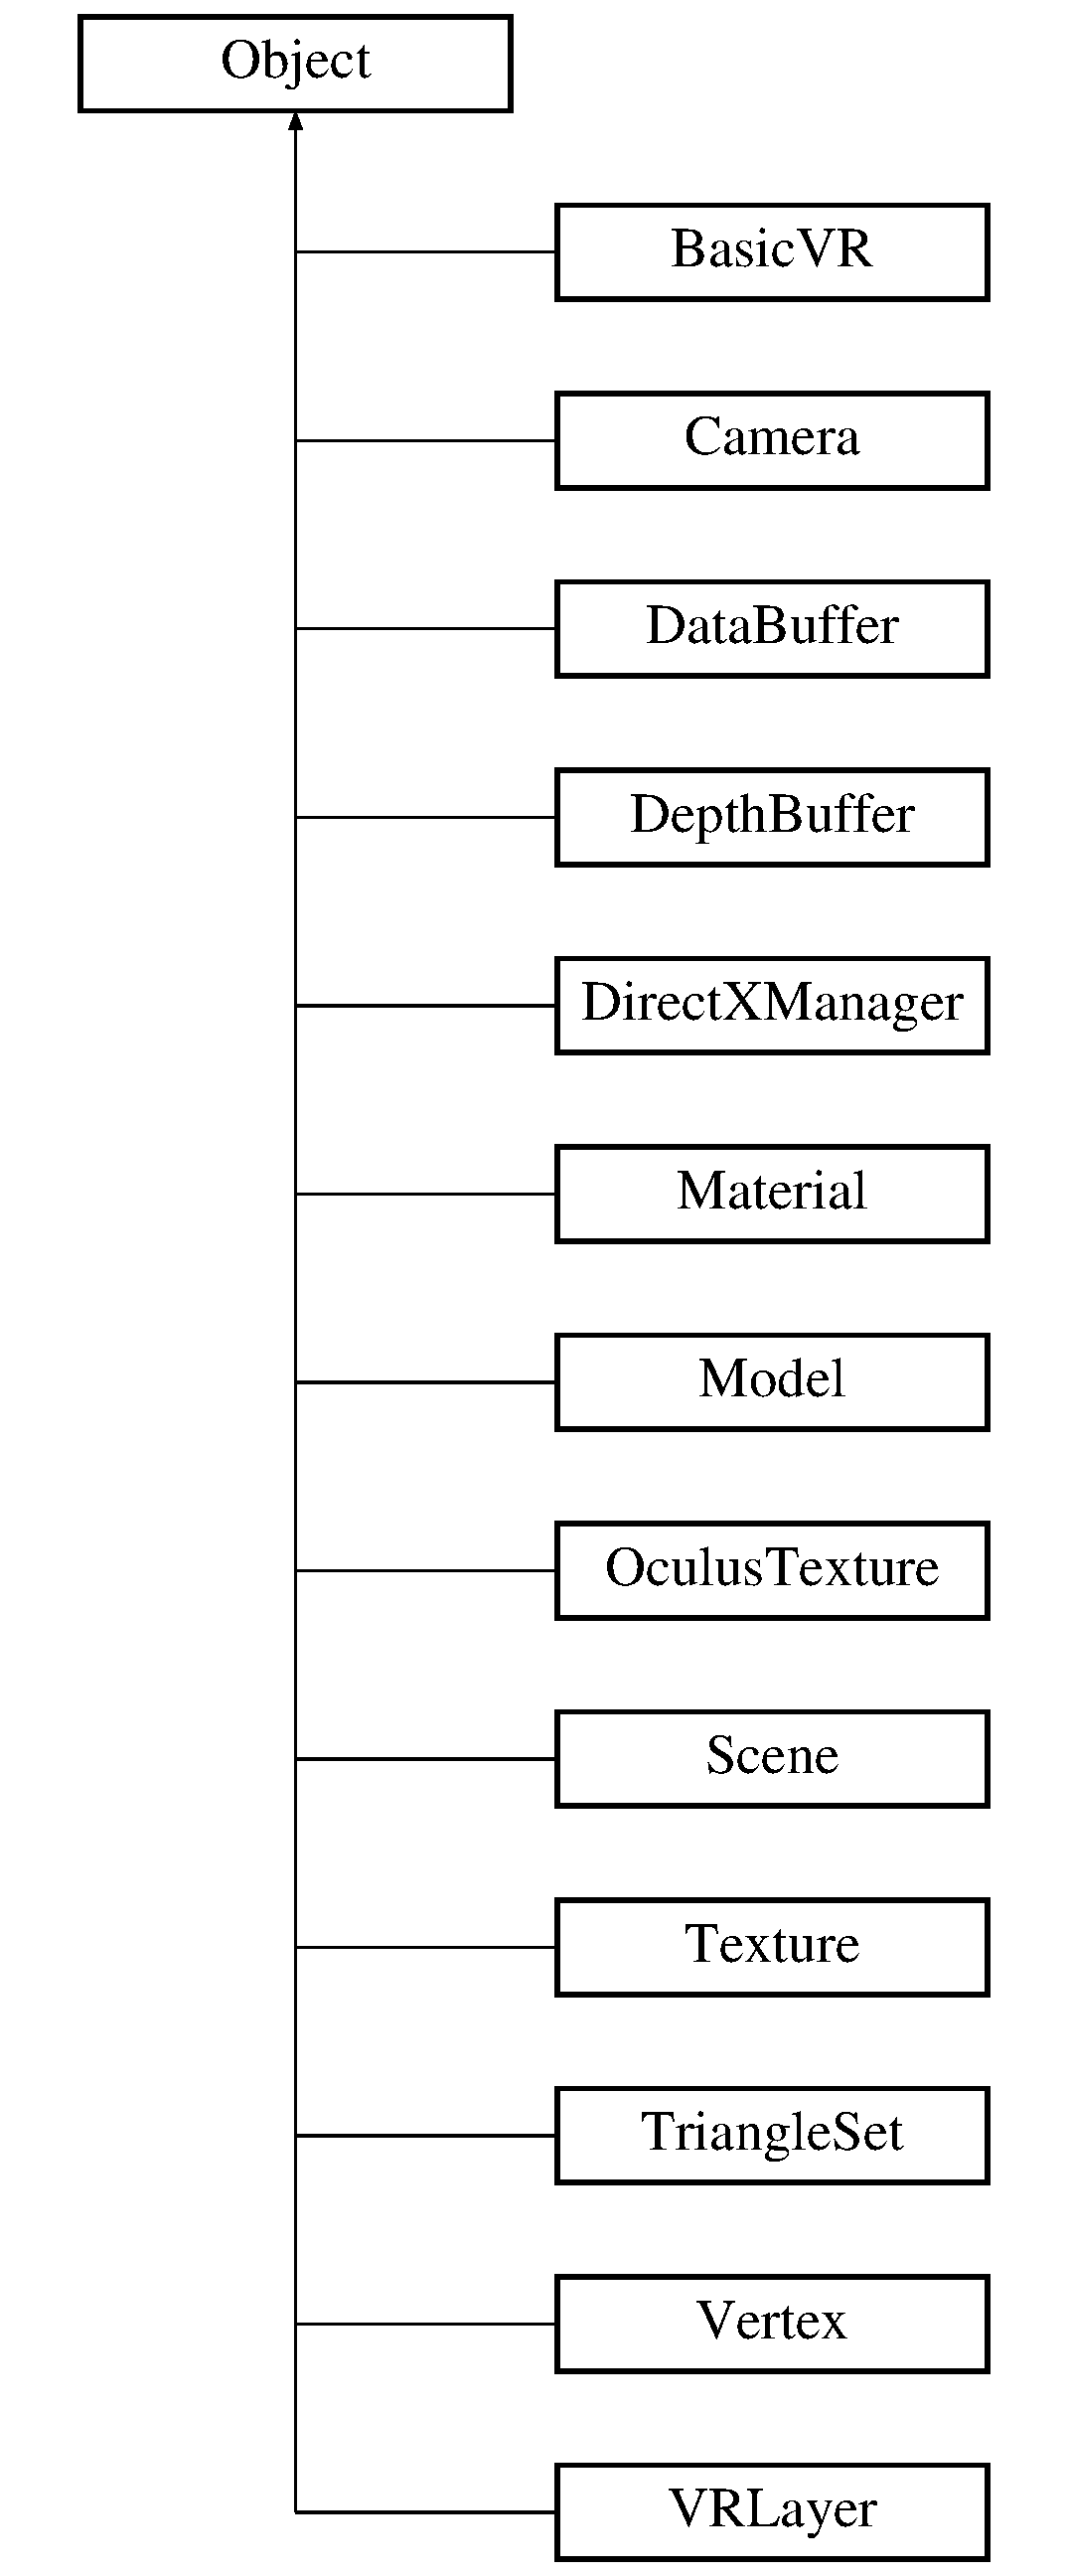
\includegraphics[height=12.000000cm]{class_object}
\end{center}
\end{figure}
\subsection*{Static Public Member Functions}
\begin{DoxyCompactItemize}
\item 
static void \hyperlink{class_object_a8a622c1336cadf4c396a75f0cabad49c}{operator delete} (void $\ast$ptr)
\begin{DoxyCompactList}\small\item\em Overloaded Operators. \end{DoxyCompactList}\item 
static void $\ast$ \hyperlink{class_object_a0369def539497b56d0b1abd4aa9f029d}{operator new} (size\+\_\+t size)
\end{DoxyCompactItemize}


\subsection{Member Function Documentation}
\index{Object@{Object}!operator delete@{operator delete}}
\index{operator delete@{operator delete}!Object@{Object}}
\subsubsection[{\texorpdfstring{operator delete(void $\ast$ptr)}{operator delete(void *ptr)}}]{\setlength{\rightskip}{0pt plus 5cm}void Object\+::operator delete (
\begin{DoxyParamCaption}
\item[{void $\ast$}]{ptr}
\end{DoxyParamCaption}
)\hspace{0.3cm}{\ttfamily [static]}}\hypertarget{class_object_a8a622c1336cadf4c396a75f0cabad49c}{}\label{class_object_a8a622c1336cadf4c396a75f0cabad49c}


Overloaded Operators. 

Uses \+\_\+aligned\+\_\+free to remove memory. All classes that inherit from \hyperlink{class_object}{Object} will use these functions when new or delete is used.

\begin{DoxyAuthor}{Author}
Katianie 
\end{DoxyAuthor}
\begin{DoxyDate}{Date}
7/4/2016
\end{DoxyDate}

\begin{DoxyParams}[1]{Parameters}
\mbox{\tt in,out}  & {\em ptr} & If non-\/null, the pointer to delete. \\
\hline
\end{DoxyParams}
\index{Object@{Object}!operator new@{operator new}}
\index{operator new@{operator new}!Object@{Object}}
\subsubsection[{\texorpdfstring{operator new(size\+\_\+t size)}{operator new(size_t size)}}]{\setlength{\rightskip}{0pt plus 5cm}void $\ast$ Object\+::operator new (
\begin{DoxyParamCaption}
\item[{size\+\_\+t}]{size}
\end{DoxyParamCaption}
)\hspace{0.3cm}{\ttfamily [static]}}\hypertarget{class_object_a0369def539497b56d0b1abd4aa9f029d}{}\label{class_object_a0369def539497b56d0b1abd4aa9f029d}
Uses \+\_\+aligned\+\_\+malloc to remove memory. All classes that inherit from \hyperlink{class_object}{Object} will use these functions when new or delete is used.

\begin{DoxyAuthor}{Author}
Katianie 
\end{DoxyAuthor}
\begin{DoxyDate}{Date}
7/4/2016
\end{DoxyDate}

\begin{DoxyParams}{Parameters}
{\em size} & The size.\\
\hline
\end{DoxyParams}
\begin{DoxyReturn}{Returns}
An aligned piece of memory. 
\end{DoxyReturn}


The documentation for this class was generated from the following files\+:\begin{DoxyCompactItemize}
\item 
Samples/\+Oculus\+Room\+Tiny\+\_\+\+Advanced/\+Common/\+Headers/\hyperlink{_object_8h}{Object.\+h}\item 
Samples/\+Oculus\+Room\+Tiny\+\_\+\+Advanced/\+Common/\+Implementations/\hyperlink{_object_8cpp}{Object.\+cpp}\end{DoxyCompactItemize}

\hypertarget{class_oculus_texture}{}\section{Oculus\+Texture Class Reference}
\label{class_oculus_texture}\index{Oculus\+Texture@{Oculus\+Texture}}


{\ttfamily \#include $<$Oculus\+Texture.\+h$>$}

Inheritance diagram for Oculus\+Texture\+:\begin{figure}[H]
\begin{center}
\leavevmode
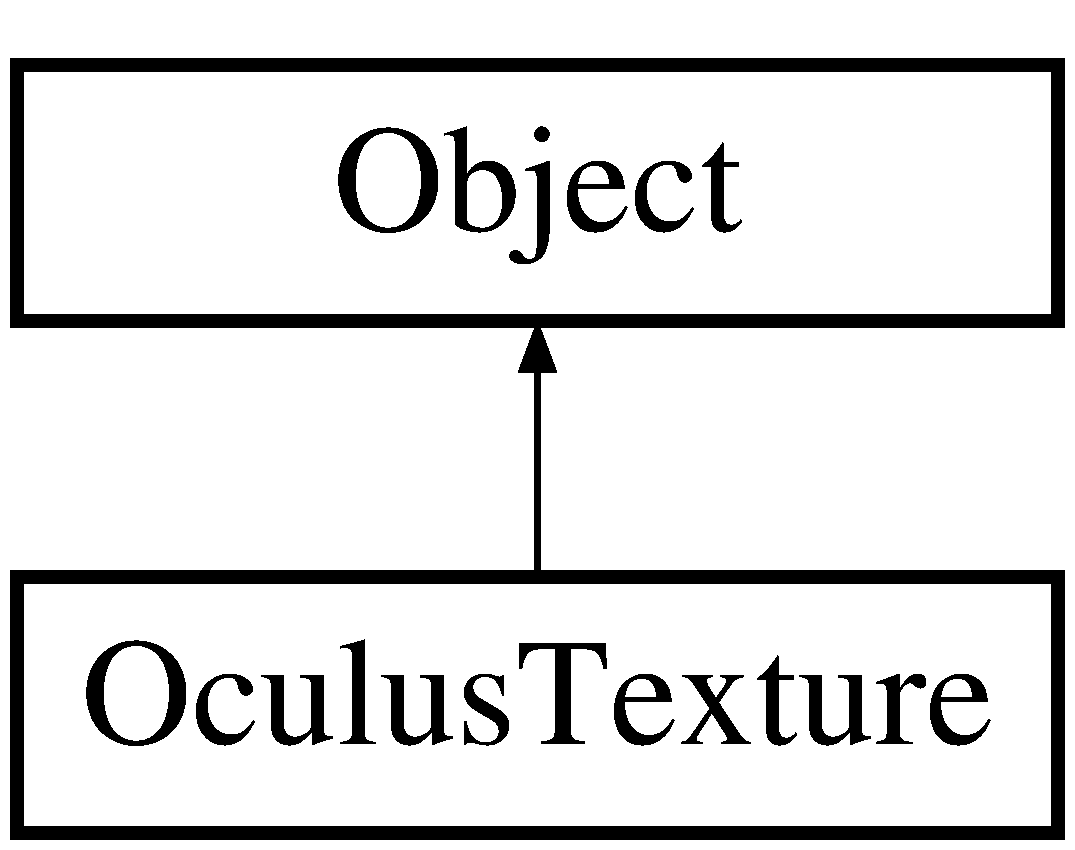
\includegraphics[height=2.000000cm]{class_oculus_texture}
\end{center}
\end{figure}
\subsection*{Public Member Functions}
\begin{DoxyCompactItemize}
\item 
\hyperlink{class_oculus_texture_ad3cc67fb9d31fe41675592f23abc5e47}{Oculus\+Texture} ()
\begin{DoxyCompactList}\small\item\em Constructors. \end{DoxyCompactList}\item 
bool \hyperlink{class_oculus_texture_a4c3211813aec38c62d198f5d2f8b5c58}{Init} (ovr\+Hmd hmd, int size\+Width, int size\+Height)
\item 
\hyperlink{class_oculus_texture_a6626d481b7b535f8aa49762bf1753071}{$\sim$\+Oculus\+Texture} ()
\begin{DoxyCompactList}\small\item\em Destructor. \end{DoxyCompactList}\item 
void \hyperlink{class_oculus_texture_afff2c510620b5aa2d2413b4fc27ce114}{Increment} ()
\begin{DoxyCompactList}\small\item\em Functions. \end{DoxyCompactList}\item 
ovr\+Hmd \hyperlink{class_oculus_texture_a3726005d9453f8616a47e735b677cb5c}{Get\+H\+MD} ()
\begin{DoxyCompactList}\small\item\em Getters. \end{DoxyCompactList}\item 
I\+D3\+D11\+Render\+Target\+View $\ast$ \hyperlink{class_oculus_texture_a17d4bcf0866848b28165ac8c0a9d77a2}{Get\+Render\+Target} (int index)
\item 
int \hyperlink{class_oculus_texture_af81b3825a506329b8db16071a5483495}{Get\+Size\+Height} ()
\item 
int \hyperlink{class_oculus_texture_af73833914f0cc424bc1dea0163ffd385}{Get\+Size\+Width} ()
\item 
ovr\+Swap\+Texture\+Set $\ast$ \hyperlink{class_oculus_texture_a826638e17b3c23dc9f9c8076726b73f3}{Get\+Swap\+Texture\+Set} ()
\end{DoxyCompactItemize}
\subsection*{Protected Attributes}
\begin{DoxyCompactItemize}
\item 
ovr\+Hmd \hyperlink{class_oculus_texture_a15c4e9c827747a8f864041baab7771ee}{my\+H\+MD}
\item 
ovr\+Swap\+Texture\+Set $\ast$ \hyperlink{class_oculus_texture_a04e78e256386bece42e85d2959d2e32f}{my\+Swap\+Texture\+Set}
\item 
I\+D3\+D11\+Render\+Target\+View $\ast$ \hyperlink{class_oculus_texture_a5d69afb8a823b45fd936437f2c0d5b87}{my\+Render\+Targets} \mbox{[}T\+E\+X\+T\+U\+R\+E\+\_\+\+C\+O\+U\+NT\mbox{]}
\item 
int \hyperlink{class_oculus_texture_afc8b36b0000c604578ad62c8ee736315}{my\+Size\+Width}
\item 
int \hyperlink{class_oculus_texture_afddb31ca4baf9069c37be3008edbb1a9}{my\+Size\+Height}
\end{DoxyCompactItemize}
\subsection*{Additional Inherited Members}


\subsection{Constructor \& Destructor Documentation}
\index{Oculus\+Texture@{Oculus\+Texture}!Oculus\+Texture@{Oculus\+Texture}}
\index{Oculus\+Texture@{Oculus\+Texture}!Oculus\+Texture@{Oculus\+Texture}}
\subsubsection[{\texorpdfstring{Oculus\+Texture()}{OculusTexture()}}]{\setlength{\rightskip}{0pt plus 5cm}Oculus\+Texture\+::\+Oculus\+Texture (
\begin{DoxyParamCaption}
{}
\end{DoxyParamCaption}
)}\hypertarget{class_oculus_texture_ad3cc67fb9d31fe41675592f23abc5e47}{}\label{class_oculus_texture_ad3cc67fb9d31fe41675592f23abc5e47}


Constructors. 

Default Constructor.

\begin{DoxyAuthor}{Author}
Katianie 
\end{DoxyAuthor}
\begin{DoxyDate}{Date}
7/4/2016 
\end{DoxyDate}
\index{Oculus\+Texture@{Oculus\+Texture}!````~Oculus\+Texture@{$\sim$\+Oculus\+Texture}}
\index{````~Oculus\+Texture@{$\sim$\+Oculus\+Texture}!Oculus\+Texture@{Oculus\+Texture}}
\subsubsection[{\texorpdfstring{$\sim$\+Oculus\+Texture()}{~OculusTexture()}}]{\setlength{\rightskip}{0pt plus 5cm}Oculus\+Texture\+::$\sim$\+Oculus\+Texture (
\begin{DoxyParamCaption}
{}
\end{DoxyParamCaption}
)}\hypertarget{class_oculus_texture_a6626d481b7b535f8aa49762bf1753071}{}\label{class_oculus_texture_a6626d481b7b535f8aa49762bf1753071}


Destructor. 

Destructor.

\begin{DoxyAuthor}{Author}
Katianie 
\end{DoxyAuthor}
\begin{DoxyDate}{Date}
7/4/2016 
\end{DoxyDate}


\subsection{Member Function Documentation}
\index{Oculus\+Texture@{Oculus\+Texture}!Get\+H\+MD@{Get\+H\+MD}}
\index{Get\+H\+MD@{Get\+H\+MD}!Oculus\+Texture@{Oculus\+Texture}}
\subsubsection[{\texorpdfstring{Get\+H\+M\+D()}{GetHMD()}}]{\setlength{\rightskip}{0pt plus 5cm}ovr\+Hmd Oculus\+Texture\+::\+Get\+H\+MD (
\begin{DoxyParamCaption}
{}
\end{DoxyParamCaption}
)}\hypertarget{class_oculus_texture_a3726005d9453f8616a47e735b677cb5c}{}\label{class_oculus_texture_a3726005d9453f8616a47e735b677cb5c}


Getters. 

Gets the H\+MD

\begin{DoxyAuthor}{Author}
Katianie 
\end{DoxyAuthor}
\begin{DoxyDate}{Date}
7/4/2016
\end{DoxyDate}
\begin{DoxyReturn}{Returns}
The H\+MD. 
\end{DoxyReturn}
\index{Oculus\+Texture@{Oculus\+Texture}!Get\+Render\+Target@{Get\+Render\+Target}}
\index{Get\+Render\+Target@{Get\+Render\+Target}!Oculus\+Texture@{Oculus\+Texture}}
\subsubsection[{\texorpdfstring{Get\+Render\+Target(int index)}{GetRenderTarget(int index)}}]{\setlength{\rightskip}{0pt plus 5cm}I\+D3\+D11\+Render\+Target\+View $\ast$ Oculus\+Texture\+::\+Get\+Render\+Target (
\begin{DoxyParamCaption}
\item[{int}]{index}
\end{DoxyParamCaption}
)}\hypertarget{class_oculus_texture_a17d4bcf0866848b28165ac8c0a9d77a2}{}\label{class_oculus_texture_a17d4bcf0866848b28165ac8c0a9d77a2}
Gets the specified Render Target.

\begin{DoxyAuthor}{Author}
Katianie 
\end{DoxyAuthor}
\begin{DoxyDate}{Date}
7/4/2016
\end{DoxyDate}

\begin{DoxyParams}{Parameters}
{\em index} & Zero-\/based index of the render target.\\
\hline
\end{DoxyParams}
\begin{DoxyReturn}{Returns}
The Render Target. 
\end{DoxyReturn}
\index{Oculus\+Texture@{Oculus\+Texture}!Get\+Size\+Height@{Get\+Size\+Height}}
\index{Get\+Size\+Height@{Get\+Size\+Height}!Oculus\+Texture@{Oculus\+Texture}}
\subsubsection[{\texorpdfstring{Get\+Size\+Height()}{GetSizeHeight()}}]{\setlength{\rightskip}{0pt plus 5cm}int Oculus\+Texture\+::\+Get\+Size\+Height (
\begin{DoxyParamCaption}
{}
\end{DoxyParamCaption}
)}\hypertarget{class_oculus_texture_af81b3825a506329b8db16071a5483495}{}\label{class_oculus_texture_af81b3825a506329b8db16071a5483495}
Gets the \hyperlink{class_texture}{Texture} height.

\begin{DoxyAuthor}{Author}
Katianie 
\end{DoxyAuthor}
\begin{DoxyDate}{Date}
7/4/2016
\end{DoxyDate}
\begin{DoxyReturn}{Returns}
The size height. 
\end{DoxyReturn}
\index{Oculus\+Texture@{Oculus\+Texture}!Get\+Size\+Width@{Get\+Size\+Width}}
\index{Get\+Size\+Width@{Get\+Size\+Width}!Oculus\+Texture@{Oculus\+Texture}}
\subsubsection[{\texorpdfstring{Get\+Size\+Width()}{GetSizeWidth()}}]{\setlength{\rightskip}{0pt plus 5cm}int Oculus\+Texture\+::\+Get\+Size\+Width (
\begin{DoxyParamCaption}
{}
\end{DoxyParamCaption}
)}\hypertarget{class_oculus_texture_af73833914f0cc424bc1dea0163ffd385}{}\label{class_oculus_texture_af73833914f0cc424bc1dea0163ffd385}
Gets the texture width.

\begin{DoxyAuthor}{Author}
Katianie 
\end{DoxyAuthor}
\begin{DoxyDate}{Date}
7/4/2016
\end{DoxyDate}
\begin{DoxyReturn}{Returns}
The \hyperlink{class_texture}{Texture} width. 
\end{DoxyReturn}
\index{Oculus\+Texture@{Oculus\+Texture}!Get\+Swap\+Texture\+Set@{Get\+Swap\+Texture\+Set}}
\index{Get\+Swap\+Texture\+Set@{Get\+Swap\+Texture\+Set}!Oculus\+Texture@{Oculus\+Texture}}
\subsubsection[{\texorpdfstring{Get\+Swap\+Texture\+Set()}{GetSwapTextureSet()}}]{\setlength{\rightskip}{0pt plus 5cm}ovr\+Swap\+Texture\+Set $\ast$ Oculus\+Texture\+::\+Get\+Swap\+Texture\+Set (
\begin{DoxyParamCaption}
{}
\end{DoxyParamCaption}
)}\hypertarget{class_oculus_texture_a826638e17b3c23dc9f9c8076726b73f3}{}\label{class_oculus_texture_a826638e17b3c23dc9f9c8076726b73f3}
Gets the Swap \hyperlink{class_texture}{Texture} Set.

\begin{DoxyAuthor}{Author}
Katianie 
\end{DoxyAuthor}
\begin{DoxyDate}{Date}
7/4/2016
\end{DoxyDate}
\begin{DoxyReturn}{Returns}
The Swap \hyperlink{class_texture}{Texture} Set. 
\end{DoxyReturn}
\index{Oculus\+Texture@{Oculus\+Texture}!Increment@{Increment}}
\index{Increment@{Increment}!Oculus\+Texture@{Oculus\+Texture}}
\subsubsection[{\texorpdfstring{Increment()}{Increment()}}]{\setlength{\rightskip}{0pt plus 5cm}void Oculus\+Texture\+::\+Increment (
\begin{DoxyParamCaption}
{}
\end{DoxyParamCaption}
)}\hypertarget{class_oculus_texture_afff2c510620b5aa2d2413b4fc27ce114}{}\label{class_oculus_texture_afff2c510620b5aa2d2413b4fc27ce114}


Functions. 

Increment the index of the current swap texture.

\begin{DoxyAuthor}{Author}
Katianie 
\end{DoxyAuthor}
\begin{DoxyDate}{Date}
7/4/2016 
\end{DoxyDate}
\index{Oculus\+Texture@{Oculus\+Texture}!Init@{Init}}
\index{Init@{Init}!Oculus\+Texture@{Oculus\+Texture}}
\subsubsection[{\texorpdfstring{Init(ovr\+Hmd hmd, int size\+Width, int size\+Height)}{Init(ovrHmd hmd, int sizeWidth, int sizeHeight)}}]{\setlength{\rightskip}{0pt plus 5cm}bool Oculus\+Texture\+::\+Init (
\begin{DoxyParamCaption}
\item[{ovr\+Hmd}]{hmd, }
\item[{int}]{size\+Width, }
\item[{int}]{size\+Height}
\end{DoxyParamCaption}
)}\hypertarget{class_oculus_texture_a4c3211813aec38c62d198f5d2f8b5c58}{}\label{class_oculus_texture_a4c3211813aec38c62d198f5d2f8b5c58}
Initializes the O\+VR \hyperlink{class_texture}{Texture} and anything related to O\+VR such as my\+Swap\+Texture\+Set.

\begin{DoxyAuthor}{Author}
Katianie 
\end{DoxyAuthor}
\begin{DoxyDate}{Date}
7/4/2016
\end{DoxyDate}

\begin{DoxyParams}{Parameters}
{\em hmd} & The H\+MD. \\
\hline
{\em size\+Width} & Width of the \hyperlink{class_texture}{Texture}. \\
\hline
{\em size\+Height} & Height of the \hyperlink{class_texture}{Texture}.\\
\hline
\end{DoxyParams}
\begin{DoxyReturn}{Returns}
true if it succeeds, false if it fails. 
\end{DoxyReturn}


\subsection{Member Data Documentation}
\index{Oculus\+Texture@{Oculus\+Texture}!my\+H\+MD@{my\+H\+MD}}
\index{my\+H\+MD@{my\+H\+MD}!Oculus\+Texture@{Oculus\+Texture}}
\subsubsection[{\texorpdfstring{my\+H\+MD}{myHMD}}]{\setlength{\rightskip}{0pt plus 5cm}ovr\+Hmd Oculus\+Texture\+::my\+H\+MD\hspace{0.3cm}{\ttfamily [protected]}}\hypertarget{class_oculus_texture_a15c4e9c827747a8f864041baab7771ee}{}\label{class_oculus_texture_a15c4e9c827747a8f864041baab7771ee}
\index{Oculus\+Texture@{Oculus\+Texture}!my\+Render\+Targets@{my\+Render\+Targets}}
\index{my\+Render\+Targets@{my\+Render\+Targets}!Oculus\+Texture@{Oculus\+Texture}}
\subsubsection[{\texorpdfstring{my\+Render\+Targets}{myRenderTargets}}]{\setlength{\rightskip}{0pt plus 5cm}I\+D3\+D11\+Render\+Target\+View$\ast$ Oculus\+Texture\+::my\+Render\+Targets\mbox{[}T\+E\+X\+T\+U\+R\+E\+\_\+\+C\+O\+U\+NT\mbox{]}\hspace{0.3cm}{\ttfamily [protected]}}\hypertarget{class_oculus_texture_a5d69afb8a823b45fd936437f2c0d5b87}{}\label{class_oculus_texture_a5d69afb8a823b45fd936437f2c0d5b87}
\index{Oculus\+Texture@{Oculus\+Texture}!my\+Size\+Height@{my\+Size\+Height}}
\index{my\+Size\+Height@{my\+Size\+Height}!Oculus\+Texture@{Oculus\+Texture}}
\subsubsection[{\texorpdfstring{my\+Size\+Height}{mySizeHeight}}]{\setlength{\rightskip}{0pt plus 5cm}int Oculus\+Texture\+::my\+Size\+Height\hspace{0.3cm}{\ttfamily [protected]}}\hypertarget{class_oculus_texture_afddb31ca4baf9069c37be3008edbb1a9}{}\label{class_oculus_texture_afddb31ca4baf9069c37be3008edbb1a9}
\index{Oculus\+Texture@{Oculus\+Texture}!my\+Size\+Width@{my\+Size\+Width}}
\index{my\+Size\+Width@{my\+Size\+Width}!Oculus\+Texture@{Oculus\+Texture}}
\subsubsection[{\texorpdfstring{my\+Size\+Width}{mySizeWidth}}]{\setlength{\rightskip}{0pt plus 5cm}int Oculus\+Texture\+::my\+Size\+Width\hspace{0.3cm}{\ttfamily [protected]}}\hypertarget{class_oculus_texture_afc8b36b0000c604578ad62c8ee736315}{}\label{class_oculus_texture_afc8b36b0000c604578ad62c8ee736315}
\index{Oculus\+Texture@{Oculus\+Texture}!my\+Swap\+Texture\+Set@{my\+Swap\+Texture\+Set}}
\index{my\+Swap\+Texture\+Set@{my\+Swap\+Texture\+Set}!Oculus\+Texture@{Oculus\+Texture}}
\subsubsection[{\texorpdfstring{my\+Swap\+Texture\+Set}{mySwapTextureSet}}]{\setlength{\rightskip}{0pt plus 5cm}ovr\+Swap\+Texture\+Set$\ast$ Oculus\+Texture\+::my\+Swap\+Texture\+Set\hspace{0.3cm}{\ttfamily [protected]}}\hypertarget{class_oculus_texture_a04e78e256386bece42e85d2959d2e32f}{}\label{class_oculus_texture_a04e78e256386bece42e85d2959d2e32f}


The documentation for this class was generated from the following files\+:\begin{DoxyCompactItemize}
\item 
Samples/\+Oculus\+Room\+Tiny\+\_\+\+Advanced/\+Common/\+Headers/\hyperlink{_oculus_texture_8h}{Oculus\+Texture.\+h}\item 
Samples/\+Oculus\+Room\+Tiny\+\_\+\+Advanced/\+Common/\+Implementations/\hyperlink{_oculus_texture_8cpp}{Oculus\+Texture.\+cpp}\end{DoxyCompactItemize}

\hypertarget{struct_o_v_r___d_d_s___h_e_a_d_e_r}{}\section{O\+V\+R\+\_\+\+D\+D\+S\+\_\+\+H\+E\+A\+D\+ER Struct Reference}
\label{struct_o_v_r___d_d_s___h_e_a_d_e_r}\index{O\+V\+R\+\_\+\+D\+D\+S\+\_\+\+H\+E\+A\+D\+ER@{O\+V\+R\+\_\+\+D\+D\+S\+\_\+\+H\+E\+A\+D\+ER}}


{\ttfamily \#include $<$Texture.\+h$>$}

\subsection*{Public Attributes}
\begin{DoxyCompactItemize}
\item 
uint32\+\_\+t \hyperlink{struct_o_v_r___d_d_s___h_e_a_d_e_r_a8c1fe9cdf1df7ef768513ea787cc69df}{Size}
\item 
uint32\+\_\+t \hyperlink{struct_o_v_r___d_d_s___h_e_a_d_e_r_a7701760de4aeb07f33e5a1141c50c334}{Flags}
\item 
uint32\+\_\+t \hyperlink{struct_o_v_r___d_d_s___h_e_a_d_e_r_aaf372cb66c243fab87315de1c4ae3715}{Height}
\item 
uint32\+\_\+t \hyperlink{struct_o_v_r___d_d_s___h_e_a_d_e_r_af4fdcef5698afebef9d5ad1270955e83}{Width}
\item 
uint32\+\_\+t \hyperlink{struct_o_v_r___d_d_s___h_e_a_d_e_r_afdf22b486a6d83b40c75485ba7dd5201}{Pitch\+Or\+Linear\+Size}
\item 
uint32\+\_\+t \hyperlink{struct_o_v_r___d_d_s___h_e_a_d_e_r_a38d00463f692dc2cb59dcec2a4fe98ab}{Depth}
\item 
uint32\+\_\+t \hyperlink{struct_o_v_r___d_d_s___h_e_a_d_e_r_a30cbe5ea75efe0dcfa9dba5b85a33181}{Mip\+Map\+Count}
\item 
uint32\+\_\+t \hyperlink{struct_o_v_r___d_d_s___h_e_a_d_e_r_a12513401bbedd0015684e76e655ce68f}{Reserved1} \mbox{[}11\mbox{]}
\item 
\hyperlink{struct_o_v_r___d_d_s___p_i_x_e_l_f_o_r_m_a_t}{O\+V\+R\+\_\+\+D\+D\+S\+\_\+\+P\+I\+X\+E\+L\+F\+O\+R\+M\+AT} \hyperlink{struct_o_v_r___d_d_s___h_e_a_d_e_r_a6dbb449fbd15f9ae6059c01c52b850f8}{Pixel\+Format}
\item 
uint32\+\_\+t \hyperlink{struct_o_v_r___d_d_s___h_e_a_d_e_r_ae26689533e4dc96fb01fbac9b134ee82}{Caps}
\item 
uint32\+\_\+t \hyperlink{struct_o_v_r___d_d_s___h_e_a_d_e_r_a46003795661aca494a01c8dfdaaabff2}{Caps2}
\item 
uint32\+\_\+t \hyperlink{struct_o_v_r___d_d_s___h_e_a_d_e_r_a7c9728203fa2e68704cbe6e26cda63bf}{Caps3}
\item 
uint32\+\_\+t \hyperlink{struct_o_v_r___d_d_s___h_e_a_d_e_r_acb1e99be9c651193f22200620496a643}{Caps4}
\item 
uint32\+\_\+t \hyperlink{struct_o_v_r___d_d_s___h_e_a_d_e_r_a84a855e10c383f3b54704891beaece9d}{Reserved2}
\end{DoxyCompactItemize}


\subsection{Member Data Documentation}
\index{O\+V\+R\+\_\+\+D\+D\+S\+\_\+\+H\+E\+A\+D\+ER@{O\+V\+R\+\_\+\+D\+D\+S\+\_\+\+H\+E\+A\+D\+ER}!Caps@{Caps}}
\index{Caps@{Caps}!O\+V\+R\+\_\+\+D\+D\+S\+\_\+\+H\+E\+A\+D\+ER@{O\+V\+R\+\_\+\+D\+D\+S\+\_\+\+H\+E\+A\+D\+ER}}
\subsubsection[{\texorpdfstring{Caps}{Caps}}]{\setlength{\rightskip}{0pt plus 5cm}uint32\+\_\+t O\+V\+R\+\_\+\+D\+D\+S\+\_\+\+H\+E\+A\+D\+E\+R\+::\+Caps}\hypertarget{struct_o_v_r___d_d_s___h_e_a_d_e_r_ae26689533e4dc96fb01fbac9b134ee82}{}\label{struct_o_v_r___d_d_s___h_e_a_d_e_r_ae26689533e4dc96fb01fbac9b134ee82}
\index{O\+V\+R\+\_\+\+D\+D\+S\+\_\+\+H\+E\+A\+D\+ER@{O\+V\+R\+\_\+\+D\+D\+S\+\_\+\+H\+E\+A\+D\+ER}!Caps2@{Caps2}}
\index{Caps2@{Caps2}!O\+V\+R\+\_\+\+D\+D\+S\+\_\+\+H\+E\+A\+D\+ER@{O\+V\+R\+\_\+\+D\+D\+S\+\_\+\+H\+E\+A\+D\+ER}}
\subsubsection[{\texorpdfstring{Caps2}{Caps2}}]{\setlength{\rightskip}{0pt plus 5cm}uint32\+\_\+t O\+V\+R\+\_\+\+D\+D\+S\+\_\+\+H\+E\+A\+D\+E\+R\+::\+Caps2}\hypertarget{struct_o_v_r___d_d_s___h_e_a_d_e_r_a46003795661aca494a01c8dfdaaabff2}{}\label{struct_o_v_r___d_d_s___h_e_a_d_e_r_a46003795661aca494a01c8dfdaaabff2}
\index{O\+V\+R\+\_\+\+D\+D\+S\+\_\+\+H\+E\+A\+D\+ER@{O\+V\+R\+\_\+\+D\+D\+S\+\_\+\+H\+E\+A\+D\+ER}!Caps3@{Caps3}}
\index{Caps3@{Caps3}!O\+V\+R\+\_\+\+D\+D\+S\+\_\+\+H\+E\+A\+D\+ER@{O\+V\+R\+\_\+\+D\+D\+S\+\_\+\+H\+E\+A\+D\+ER}}
\subsubsection[{\texorpdfstring{Caps3}{Caps3}}]{\setlength{\rightskip}{0pt plus 5cm}uint32\+\_\+t O\+V\+R\+\_\+\+D\+D\+S\+\_\+\+H\+E\+A\+D\+E\+R\+::\+Caps3}\hypertarget{struct_o_v_r___d_d_s___h_e_a_d_e_r_a7c9728203fa2e68704cbe6e26cda63bf}{}\label{struct_o_v_r___d_d_s___h_e_a_d_e_r_a7c9728203fa2e68704cbe6e26cda63bf}
\index{O\+V\+R\+\_\+\+D\+D\+S\+\_\+\+H\+E\+A\+D\+ER@{O\+V\+R\+\_\+\+D\+D\+S\+\_\+\+H\+E\+A\+D\+ER}!Caps4@{Caps4}}
\index{Caps4@{Caps4}!O\+V\+R\+\_\+\+D\+D\+S\+\_\+\+H\+E\+A\+D\+ER@{O\+V\+R\+\_\+\+D\+D\+S\+\_\+\+H\+E\+A\+D\+ER}}
\subsubsection[{\texorpdfstring{Caps4}{Caps4}}]{\setlength{\rightskip}{0pt plus 5cm}uint32\+\_\+t O\+V\+R\+\_\+\+D\+D\+S\+\_\+\+H\+E\+A\+D\+E\+R\+::\+Caps4}\hypertarget{struct_o_v_r___d_d_s___h_e_a_d_e_r_acb1e99be9c651193f22200620496a643}{}\label{struct_o_v_r___d_d_s___h_e_a_d_e_r_acb1e99be9c651193f22200620496a643}
\index{O\+V\+R\+\_\+\+D\+D\+S\+\_\+\+H\+E\+A\+D\+ER@{O\+V\+R\+\_\+\+D\+D\+S\+\_\+\+H\+E\+A\+D\+ER}!Depth@{Depth}}
\index{Depth@{Depth}!O\+V\+R\+\_\+\+D\+D\+S\+\_\+\+H\+E\+A\+D\+ER@{O\+V\+R\+\_\+\+D\+D\+S\+\_\+\+H\+E\+A\+D\+ER}}
\subsubsection[{\texorpdfstring{Depth}{Depth}}]{\setlength{\rightskip}{0pt plus 5cm}uint32\+\_\+t O\+V\+R\+\_\+\+D\+D\+S\+\_\+\+H\+E\+A\+D\+E\+R\+::\+Depth}\hypertarget{struct_o_v_r___d_d_s___h_e_a_d_e_r_a38d00463f692dc2cb59dcec2a4fe98ab}{}\label{struct_o_v_r___d_d_s___h_e_a_d_e_r_a38d00463f692dc2cb59dcec2a4fe98ab}
\index{O\+V\+R\+\_\+\+D\+D\+S\+\_\+\+H\+E\+A\+D\+ER@{O\+V\+R\+\_\+\+D\+D\+S\+\_\+\+H\+E\+A\+D\+ER}!Flags@{Flags}}
\index{Flags@{Flags}!O\+V\+R\+\_\+\+D\+D\+S\+\_\+\+H\+E\+A\+D\+ER@{O\+V\+R\+\_\+\+D\+D\+S\+\_\+\+H\+E\+A\+D\+ER}}
\subsubsection[{\texorpdfstring{Flags}{Flags}}]{\setlength{\rightskip}{0pt plus 5cm}uint32\+\_\+t O\+V\+R\+\_\+\+D\+D\+S\+\_\+\+H\+E\+A\+D\+E\+R\+::\+Flags}\hypertarget{struct_o_v_r___d_d_s___h_e_a_d_e_r_a7701760de4aeb07f33e5a1141c50c334}{}\label{struct_o_v_r___d_d_s___h_e_a_d_e_r_a7701760de4aeb07f33e5a1141c50c334}
\index{O\+V\+R\+\_\+\+D\+D\+S\+\_\+\+H\+E\+A\+D\+ER@{O\+V\+R\+\_\+\+D\+D\+S\+\_\+\+H\+E\+A\+D\+ER}!Height@{Height}}
\index{Height@{Height}!O\+V\+R\+\_\+\+D\+D\+S\+\_\+\+H\+E\+A\+D\+ER@{O\+V\+R\+\_\+\+D\+D\+S\+\_\+\+H\+E\+A\+D\+ER}}
\subsubsection[{\texorpdfstring{Height}{Height}}]{\setlength{\rightskip}{0pt plus 5cm}uint32\+\_\+t O\+V\+R\+\_\+\+D\+D\+S\+\_\+\+H\+E\+A\+D\+E\+R\+::\+Height}\hypertarget{struct_o_v_r___d_d_s___h_e_a_d_e_r_aaf372cb66c243fab87315de1c4ae3715}{}\label{struct_o_v_r___d_d_s___h_e_a_d_e_r_aaf372cb66c243fab87315de1c4ae3715}
\index{O\+V\+R\+\_\+\+D\+D\+S\+\_\+\+H\+E\+A\+D\+ER@{O\+V\+R\+\_\+\+D\+D\+S\+\_\+\+H\+E\+A\+D\+ER}!Mip\+Map\+Count@{Mip\+Map\+Count}}
\index{Mip\+Map\+Count@{Mip\+Map\+Count}!O\+V\+R\+\_\+\+D\+D\+S\+\_\+\+H\+E\+A\+D\+ER@{O\+V\+R\+\_\+\+D\+D\+S\+\_\+\+H\+E\+A\+D\+ER}}
\subsubsection[{\texorpdfstring{Mip\+Map\+Count}{MipMapCount}}]{\setlength{\rightskip}{0pt plus 5cm}uint32\+\_\+t O\+V\+R\+\_\+\+D\+D\+S\+\_\+\+H\+E\+A\+D\+E\+R\+::\+Mip\+Map\+Count}\hypertarget{struct_o_v_r___d_d_s___h_e_a_d_e_r_a30cbe5ea75efe0dcfa9dba5b85a33181}{}\label{struct_o_v_r___d_d_s___h_e_a_d_e_r_a30cbe5ea75efe0dcfa9dba5b85a33181}
\index{O\+V\+R\+\_\+\+D\+D\+S\+\_\+\+H\+E\+A\+D\+ER@{O\+V\+R\+\_\+\+D\+D\+S\+\_\+\+H\+E\+A\+D\+ER}!Pitch\+Or\+Linear\+Size@{Pitch\+Or\+Linear\+Size}}
\index{Pitch\+Or\+Linear\+Size@{Pitch\+Or\+Linear\+Size}!O\+V\+R\+\_\+\+D\+D\+S\+\_\+\+H\+E\+A\+D\+ER@{O\+V\+R\+\_\+\+D\+D\+S\+\_\+\+H\+E\+A\+D\+ER}}
\subsubsection[{\texorpdfstring{Pitch\+Or\+Linear\+Size}{PitchOrLinearSize}}]{\setlength{\rightskip}{0pt plus 5cm}uint32\+\_\+t O\+V\+R\+\_\+\+D\+D\+S\+\_\+\+H\+E\+A\+D\+E\+R\+::\+Pitch\+Or\+Linear\+Size}\hypertarget{struct_o_v_r___d_d_s___h_e_a_d_e_r_afdf22b486a6d83b40c75485ba7dd5201}{}\label{struct_o_v_r___d_d_s___h_e_a_d_e_r_afdf22b486a6d83b40c75485ba7dd5201}
\index{O\+V\+R\+\_\+\+D\+D\+S\+\_\+\+H\+E\+A\+D\+ER@{O\+V\+R\+\_\+\+D\+D\+S\+\_\+\+H\+E\+A\+D\+ER}!Pixel\+Format@{Pixel\+Format}}
\index{Pixel\+Format@{Pixel\+Format}!O\+V\+R\+\_\+\+D\+D\+S\+\_\+\+H\+E\+A\+D\+ER@{O\+V\+R\+\_\+\+D\+D\+S\+\_\+\+H\+E\+A\+D\+ER}}
\subsubsection[{\texorpdfstring{Pixel\+Format}{PixelFormat}}]{\setlength{\rightskip}{0pt plus 5cm}{\bf O\+V\+R\+\_\+\+D\+D\+S\+\_\+\+P\+I\+X\+E\+L\+F\+O\+R\+M\+AT} O\+V\+R\+\_\+\+D\+D\+S\+\_\+\+H\+E\+A\+D\+E\+R\+::\+Pixel\+Format}\hypertarget{struct_o_v_r___d_d_s___h_e_a_d_e_r_a6dbb449fbd15f9ae6059c01c52b850f8}{}\label{struct_o_v_r___d_d_s___h_e_a_d_e_r_a6dbb449fbd15f9ae6059c01c52b850f8}
\index{O\+V\+R\+\_\+\+D\+D\+S\+\_\+\+H\+E\+A\+D\+ER@{O\+V\+R\+\_\+\+D\+D\+S\+\_\+\+H\+E\+A\+D\+ER}!Reserved1@{Reserved1}}
\index{Reserved1@{Reserved1}!O\+V\+R\+\_\+\+D\+D\+S\+\_\+\+H\+E\+A\+D\+ER@{O\+V\+R\+\_\+\+D\+D\+S\+\_\+\+H\+E\+A\+D\+ER}}
\subsubsection[{\texorpdfstring{Reserved1}{Reserved1}}]{\setlength{\rightskip}{0pt plus 5cm}uint32\+\_\+t O\+V\+R\+\_\+\+D\+D\+S\+\_\+\+H\+E\+A\+D\+E\+R\+::\+Reserved1\mbox{[}11\mbox{]}}\hypertarget{struct_o_v_r___d_d_s___h_e_a_d_e_r_a12513401bbedd0015684e76e655ce68f}{}\label{struct_o_v_r___d_d_s___h_e_a_d_e_r_a12513401bbedd0015684e76e655ce68f}
\index{O\+V\+R\+\_\+\+D\+D\+S\+\_\+\+H\+E\+A\+D\+ER@{O\+V\+R\+\_\+\+D\+D\+S\+\_\+\+H\+E\+A\+D\+ER}!Reserved2@{Reserved2}}
\index{Reserved2@{Reserved2}!O\+V\+R\+\_\+\+D\+D\+S\+\_\+\+H\+E\+A\+D\+ER@{O\+V\+R\+\_\+\+D\+D\+S\+\_\+\+H\+E\+A\+D\+ER}}
\subsubsection[{\texorpdfstring{Reserved2}{Reserved2}}]{\setlength{\rightskip}{0pt plus 5cm}uint32\+\_\+t O\+V\+R\+\_\+\+D\+D\+S\+\_\+\+H\+E\+A\+D\+E\+R\+::\+Reserved2}\hypertarget{struct_o_v_r___d_d_s___h_e_a_d_e_r_a84a855e10c383f3b54704891beaece9d}{}\label{struct_o_v_r___d_d_s___h_e_a_d_e_r_a84a855e10c383f3b54704891beaece9d}
\index{O\+V\+R\+\_\+\+D\+D\+S\+\_\+\+H\+E\+A\+D\+ER@{O\+V\+R\+\_\+\+D\+D\+S\+\_\+\+H\+E\+A\+D\+ER}!Size@{Size}}
\index{Size@{Size}!O\+V\+R\+\_\+\+D\+D\+S\+\_\+\+H\+E\+A\+D\+ER@{O\+V\+R\+\_\+\+D\+D\+S\+\_\+\+H\+E\+A\+D\+ER}}
\subsubsection[{\texorpdfstring{Size}{Size}}]{\setlength{\rightskip}{0pt plus 5cm}uint32\+\_\+t O\+V\+R\+\_\+\+D\+D\+S\+\_\+\+H\+E\+A\+D\+E\+R\+::\+Size}\hypertarget{struct_o_v_r___d_d_s___h_e_a_d_e_r_a8c1fe9cdf1df7ef768513ea787cc69df}{}\label{struct_o_v_r___d_d_s___h_e_a_d_e_r_a8c1fe9cdf1df7ef768513ea787cc69df}
\index{O\+V\+R\+\_\+\+D\+D\+S\+\_\+\+H\+E\+A\+D\+ER@{O\+V\+R\+\_\+\+D\+D\+S\+\_\+\+H\+E\+A\+D\+ER}!Width@{Width}}
\index{Width@{Width}!O\+V\+R\+\_\+\+D\+D\+S\+\_\+\+H\+E\+A\+D\+ER@{O\+V\+R\+\_\+\+D\+D\+S\+\_\+\+H\+E\+A\+D\+ER}}
\subsubsection[{\texorpdfstring{Width}{Width}}]{\setlength{\rightskip}{0pt plus 5cm}uint32\+\_\+t O\+V\+R\+\_\+\+D\+D\+S\+\_\+\+H\+E\+A\+D\+E\+R\+::\+Width}\hypertarget{struct_o_v_r___d_d_s___h_e_a_d_e_r_af4fdcef5698afebef9d5ad1270955e83}{}\label{struct_o_v_r___d_d_s___h_e_a_d_e_r_af4fdcef5698afebef9d5ad1270955e83}


The documentation for this struct was generated from the following file\+:\begin{DoxyCompactItemize}
\item 
Samples/\+Oculus\+Room\+Tiny\+\_\+\+Advanced/\+Common/\+Headers/\hyperlink{_texture_8h}{Texture.\+h}\end{DoxyCompactItemize}

\hypertarget{struct_o_v_r___d_d_s___p_i_x_e_l_f_o_r_m_a_t}{}\section{O\+V\+R\+\_\+\+D\+D\+S\+\_\+\+P\+I\+X\+E\+L\+F\+O\+R\+M\+AT Struct Reference}
\label{struct_o_v_r___d_d_s___p_i_x_e_l_f_o_r_m_a_t}\index{O\+V\+R\+\_\+\+D\+D\+S\+\_\+\+P\+I\+X\+E\+L\+F\+O\+R\+M\+AT@{O\+V\+R\+\_\+\+D\+D\+S\+\_\+\+P\+I\+X\+E\+L\+F\+O\+R\+M\+AT}}


{\ttfamily \#include $<$Texture.\+h$>$}

\subsection*{Public Attributes}
\begin{DoxyCompactItemize}
\item 
uint32\+\_\+t \hyperlink{struct_o_v_r___d_d_s___p_i_x_e_l_f_o_r_m_a_t_a36e9f53f78969fa1f1fc7c3424e9564a}{Size}
\item 
uint32\+\_\+t \hyperlink{struct_o_v_r___d_d_s___p_i_x_e_l_f_o_r_m_a_t_a5966f309452d940a4b3ec2cdd169c2fa}{Flags}
\item 
uint32\+\_\+t \hyperlink{struct_o_v_r___d_d_s___p_i_x_e_l_f_o_r_m_a_t_a5b9de7de2eb937c472723d66f240de27}{Four\+CC}
\item 
uint32\+\_\+t \hyperlink{struct_o_v_r___d_d_s___p_i_x_e_l_f_o_r_m_a_t_a3986b797ae77fd2a274744bf93d6626a}{R\+G\+B\+Bit\+Count}
\item 
uint32\+\_\+t \hyperlink{struct_o_v_r___d_d_s___p_i_x_e_l_f_o_r_m_a_t_a3bcaa8b8745f43597deef9248408a96e}{R\+Bit\+Mask}
\item 
uint32\+\_\+t \hyperlink{struct_o_v_r___d_d_s___p_i_x_e_l_f_o_r_m_a_t_a91d43b30eaf50f2eb51ccf500f490793}{G\+Bit\+Mask}
\item 
uint32\+\_\+t \hyperlink{struct_o_v_r___d_d_s___p_i_x_e_l_f_o_r_m_a_t_a4e0f0dd4720c4caf65575223840ab60f}{B\+Bit\+Mask}
\item 
uint32\+\_\+t \hyperlink{struct_o_v_r___d_d_s___p_i_x_e_l_f_o_r_m_a_t_a02aee0d907d689d0116794f08af92670}{A\+Bit\+Mask}
\end{DoxyCompactItemize}


\subsection{Member Data Documentation}
\index{O\+V\+R\+\_\+\+D\+D\+S\+\_\+\+P\+I\+X\+E\+L\+F\+O\+R\+M\+AT@{O\+V\+R\+\_\+\+D\+D\+S\+\_\+\+P\+I\+X\+E\+L\+F\+O\+R\+M\+AT}!A\+Bit\+Mask@{A\+Bit\+Mask}}
\index{A\+Bit\+Mask@{A\+Bit\+Mask}!O\+V\+R\+\_\+\+D\+D\+S\+\_\+\+P\+I\+X\+E\+L\+F\+O\+R\+M\+AT@{O\+V\+R\+\_\+\+D\+D\+S\+\_\+\+P\+I\+X\+E\+L\+F\+O\+R\+M\+AT}}
\subsubsection[{\texorpdfstring{A\+Bit\+Mask}{ABitMask}}]{\setlength{\rightskip}{0pt plus 5cm}uint32\+\_\+t O\+V\+R\+\_\+\+D\+D\+S\+\_\+\+P\+I\+X\+E\+L\+F\+O\+R\+M\+A\+T\+::\+A\+Bit\+Mask}\hypertarget{struct_o_v_r___d_d_s___p_i_x_e_l_f_o_r_m_a_t_a02aee0d907d689d0116794f08af92670}{}\label{struct_o_v_r___d_d_s___p_i_x_e_l_f_o_r_m_a_t_a02aee0d907d689d0116794f08af92670}
\index{O\+V\+R\+\_\+\+D\+D\+S\+\_\+\+P\+I\+X\+E\+L\+F\+O\+R\+M\+AT@{O\+V\+R\+\_\+\+D\+D\+S\+\_\+\+P\+I\+X\+E\+L\+F\+O\+R\+M\+AT}!B\+Bit\+Mask@{B\+Bit\+Mask}}
\index{B\+Bit\+Mask@{B\+Bit\+Mask}!O\+V\+R\+\_\+\+D\+D\+S\+\_\+\+P\+I\+X\+E\+L\+F\+O\+R\+M\+AT@{O\+V\+R\+\_\+\+D\+D\+S\+\_\+\+P\+I\+X\+E\+L\+F\+O\+R\+M\+AT}}
\subsubsection[{\texorpdfstring{B\+Bit\+Mask}{BBitMask}}]{\setlength{\rightskip}{0pt plus 5cm}uint32\+\_\+t O\+V\+R\+\_\+\+D\+D\+S\+\_\+\+P\+I\+X\+E\+L\+F\+O\+R\+M\+A\+T\+::\+B\+Bit\+Mask}\hypertarget{struct_o_v_r___d_d_s___p_i_x_e_l_f_o_r_m_a_t_a4e0f0dd4720c4caf65575223840ab60f}{}\label{struct_o_v_r___d_d_s___p_i_x_e_l_f_o_r_m_a_t_a4e0f0dd4720c4caf65575223840ab60f}
\index{O\+V\+R\+\_\+\+D\+D\+S\+\_\+\+P\+I\+X\+E\+L\+F\+O\+R\+M\+AT@{O\+V\+R\+\_\+\+D\+D\+S\+\_\+\+P\+I\+X\+E\+L\+F\+O\+R\+M\+AT}!Flags@{Flags}}
\index{Flags@{Flags}!O\+V\+R\+\_\+\+D\+D\+S\+\_\+\+P\+I\+X\+E\+L\+F\+O\+R\+M\+AT@{O\+V\+R\+\_\+\+D\+D\+S\+\_\+\+P\+I\+X\+E\+L\+F\+O\+R\+M\+AT}}
\subsubsection[{\texorpdfstring{Flags}{Flags}}]{\setlength{\rightskip}{0pt plus 5cm}uint32\+\_\+t O\+V\+R\+\_\+\+D\+D\+S\+\_\+\+P\+I\+X\+E\+L\+F\+O\+R\+M\+A\+T\+::\+Flags}\hypertarget{struct_o_v_r___d_d_s___p_i_x_e_l_f_o_r_m_a_t_a5966f309452d940a4b3ec2cdd169c2fa}{}\label{struct_o_v_r___d_d_s___p_i_x_e_l_f_o_r_m_a_t_a5966f309452d940a4b3ec2cdd169c2fa}
\index{O\+V\+R\+\_\+\+D\+D\+S\+\_\+\+P\+I\+X\+E\+L\+F\+O\+R\+M\+AT@{O\+V\+R\+\_\+\+D\+D\+S\+\_\+\+P\+I\+X\+E\+L\+F\+O\+R\+M\+AT}!Four\+CC@{Four\+CC}}
\index{Four\+CC@{Four\+CC}!O\+V\+R\+\_\+\+D\+D\+S\+\_\+\+P\+I\+X\+E\+L\+F\+O\+R\+M\+AT@{O\+V\+R\+\_\+\+D\+D\+S\+\_\+\+P\+I\+X\+E\+L\+F\+O\+R\+M\+AT}}
\subsubsection[{\texorpdfstring{Four\+CC}{FourCC}}]{\setlength{\rightskip}{0pt plus 5cm}uint32\+\_\+t O\+V\+R\+\_\+\+D\+D\+S\+\_\+\+P\+I\+X\+E\+L\+F\+O\+R\+M\+A\+T\+::\+Four\+CC}\hypertarget{struct_o_v_r___d_d_s___p_i_x_e_l_f_o_r_m_a_t_a5b9de7de2eb937c472723d66f240de27}{}\label{struct_o_v_r___d_d_s___p_i_x_e_l_f_o_r_m_a_t_a5b9de7de2eb937c472723d66f240de27}
\index{O\+V\+R\+\_\+\+D\+D\+S\+\_\+\+P\+I\+X\+E\+L\+F\+O\+R\+M\+AT@{O\+V\+R\+\_\+\+D\+D\+S\+\_\+\+P\+I\+X\+E\+L\+F\+O\+R\+M\+AT}!G\+Bit\+Mask@{G\+Bit\+Mask}}
\index{G\+Bit\+Mask@{G\+Bit\+Mask}!O\+V\+R\+\_\+\+D\+D\+S\+\_\+\+P\+I\+X\+E\+L\+F\+O\+R\+M\+AT@{O\+V\+R\+\_\+\+D\+D\+S\+\_\+\+P\+I\+X\+E\+L\+F\+O\+R\+M\+AT}}
\subsubsection[{\texorpdfstring{G\+Bit\+Mask}{GBitMask}}]{\setlength{\rightskip}{0pt plus 5cm}uint32\+\_\+t O\+V\+R\+\_\+\+D\+D\+S\+\_\+\+P\+I\+X\+E\+L\+F\+O\+R\+M\+A\+T\+::\+G\+Bit\+Mask}\hypertarget{struct_o_v_r___d_d_s___p_i_x_e_l_f_o_r_m_a_t_a91d43b30eaf50f2eb51ccf500f490793}{}\label{struct_o_v_r___d_d_s___p_i_x_e_l_f_o_r_m_a_t_a91d43b30eaf50f2eb51ccf500f490793}
\index{O\+V\+R\+\_\+\+D\+D\+S\+\_\+\+P\+I\+X\+E\+L\+F\+O\+R\+M\+AT@{O\+V\+R\+\_\+\+D\+D\+S\+\_\+\+P\+I\+X\+E\+L\+F\+O\+R\+M\+AT}!R\+Bit\+Mask@{R\+Bit\+Mask}}
\index{R\+Bit\+Mask@{R\+Bit\+Mask}!O\+V\+R\+\_\+\+D\+D\+S\+\_\+\+P\+I\+X\+E\+L\+F\+O\+R\+M\+AT@{O\+V\+R\+\_\+\+D\+D\+S\+\_\+\+P\+I\+X\+E\+L\+F\+O\+R\+M\+AT}}
\subsubsection[{\texorpdfstring{R\+Bit\+Mask}{RBitMask}}]{\setlength{\rightskip}{0pt plus 5cm}uint32\+\_\+t O\+V\+R\+\_\+\+D\+D\+S\+\_\+\+P\+I\+X\+E\+L\+F\+O\+R\+M\+A\+T\+::\+R\+Bit\+Mask}\hypertarget{struct_o_v_r___d_d_s___p_i_x_e_l_f_o_r_m_a_t_a3bcaa8b8745f43597deef9248408a96e}{}\label{struct_o_v_r___d_d_s___p_i_x_e_l_f_o_r_m_a_t_a3bcaa8b8745f43597deef9248408a96e}
\index{O\+V\+R\+\_\+\+D\+D\+S\+\_\+\+P\+I\+X\+E\+L\+F\+O\+R\+M\+AT@{O\+V\+R\+\_\+\+D\+D\+S\+\_\+\+P\+I\+X\+E\+L\+F\+O\+R\+M\+AT}!R\+G\+B\+Bit\+Count@{R\+G\+B\+Bit\+Count}}
\index{R\+G\+B\+Bit\+Count@{R\+G\+B\+Bit\+Count}!O\+V\+R\+\_\+\+D\+D\+S\+\_\+\+P\+I\+X\+E\+L\+F\+O\+R\+M\+AT@{O\+V\+R\+\_\+\+D\+D\+S\+\_\+\+P\+I\+X\+E\+L\+F\+O\+R\+M\+AT}}
\subsubsection[{\texorpdfstring{R\+G\+B\+Bit\+Count}{RGBBitCount}}]{\setlength{\rightskip}{0pt plus 5cm}uint32\+\_\+t O\+V\+R\+\_\+\+D\+D\+S\+\_\+\+P\+I\+X\+E\+L\+F\+O\+R\+M\+A\+T\+::\+R\+G\+B\+Bit\+Count}\hypertarget{struct_o_v_r___d_d_s___p_i_x_e_l_f_o_r_m_a_t_a3986b797ae77fd2a274744bf93d6626a}{}\label{struct_o_v_r___d_d_s___p_i_x_e_l_f_o_r_m_a_t_a3986b797ae77fd2a274744bf93d6626a}
\index{O\+V\+R\+\_\+\+D\+D\+S\+\_\+\+P\+I\+X\+E\+L\+F\+O\+R\+M\+AT@{O\+V\+R\+\_\+\+D\+D\+S\+\_\+\+P\+I\+X\+E\+L\+F\+O\+R\+M\+AT}!Size@{Size}}
\index{Size@{Size}!O\+V\+R\+\_\+\+D\+D\+S\+\_\+\+P\+I\+X\+E\+L\+F\+O\+R\+M\+AT@{O\+V\+R\+\_\+\+D\+D\+S\+\_\+\+P\+I\+X\+E\+L\+F\+O\+R\+M\+AT}}
\subsubsection[{\texorpdfstring{Size}{Size}}]{\setlength{\rightskip}{0pt plus 5cm}uint32\+\_\+t O\+V\+R\+\_\+\+D\+D\+S\+\_\+\+P\+I\+X\+E\+L\+F\+O\+R\+M\+A\+T\+::\+Size}\hypertarget{struct_o_v_r___d_d_s___p_i_x_e_l_f_o_r_m_a_t_a36e9f53f78969fa1f1fc7c3424e9564a}{}\label{struct_o_v_r___d_d_s___p_i_x_e_l_f_o_r_m_a_t_a36e9f53f78969fa1f1fc7c3424e9564a}


The documentation for this struct was generated from the following file\+:\begin{DoxyCompactItemize}
\item 
Samples/\+Oculus\+Room\+Tiny\+\_\+\+Advanced/\+Common/\+Headers/\hyperlink{_texture_8h}{Texture.\+h}\end{DoxyCompactItemize}

\hypertarget{class_scene}{}\section{Scene Class Reference}
\label{class_scene}\index{Scene@{Scene}}


{\ttfamily \#include $<$Scene.\+h$>$}

Inheritance diagram for Scene\+:\begin{figure}[H]
\begin{center}
\leavevmode
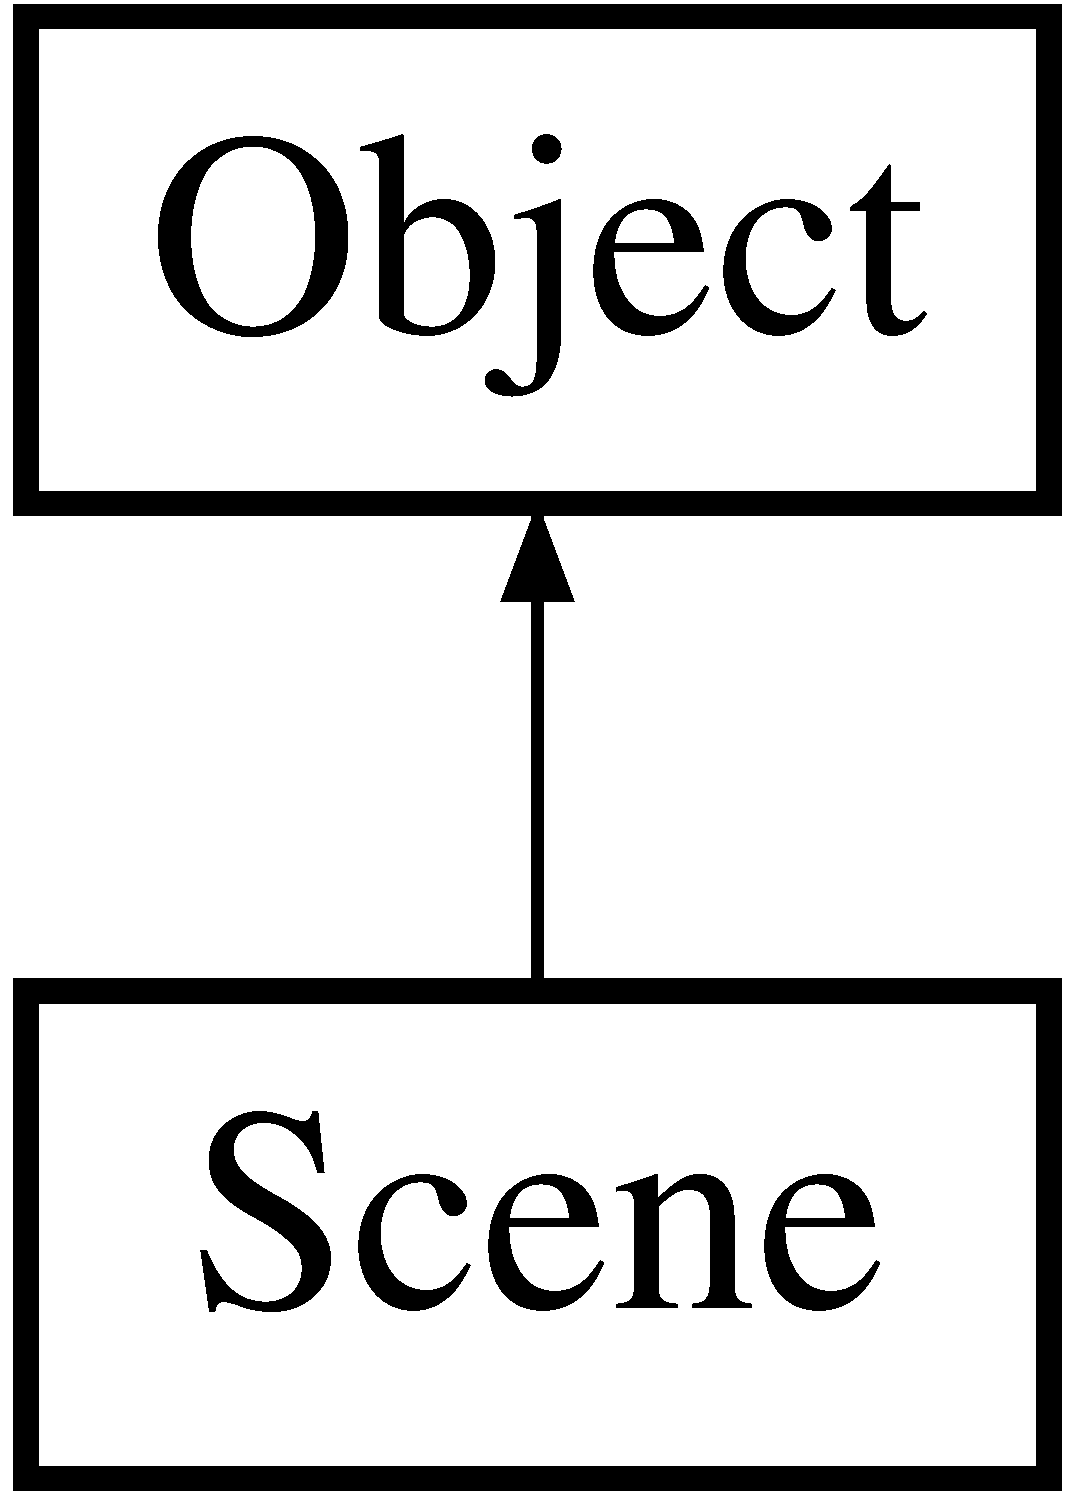
\includegraphics[height=2.000000cm]{class_scene}
\end{center}
\end{figure}
\subsection*{Public Member Functions}
\begin{DoxyCompactItemize}
\item 
\hyperlink{class_scene_afba62439dfcdf3b5bcbce46635ea0dd8}{Scene} (char $\ast$image\+File\+Path, char $\ast$txt\+Tool\+Path, char $\ast$output\+Path, char $\ast$config\+File\+Path, char $\ast$vertex\+Shader\+Path, char $\ast$pixel\+Shader\+Path)
\begin{DoxyCompactList}\small\item\em Constructors. \end{DoxyCompactList}\item 
void \hyperlink{class_scene_a1f36ab9f3f9c1286e79e63c37ca0580f}{Init} (char $\ast$image\+File\+Path, char $\ast$txt\+Tool\+Path, char $\ast$output\+Path, char $\ast$config\+File\+Path, char $\ast$vertex\+Shader\+Path, char $\ast$pixel\+Shader\+Path)
\item 
virtual \hyperlink{class_scene_a3b8cec2e32546713915f8c6303c951f1}{$\sim$\+Scene} ()
\begin{DoxyCompactList}\small\item\em Destructor. \end{DoxyCompactList}\item 
float \hyperlink{class_scene_abf429ee85b796b169893ffaf06175135}{Calculate\+Ideal\+Panoramic\+Height} (int panoramic\+Type, float texture\+Height)
\begin{DoxyCompactList}\small\item\em Functions. \end{DoxyCompactList}\item 
float \hyperlink{class_scene_af396d1333d3b5962f9f8e35bf9d32a6e}{Calculate\+Ideal\+Panoramic\+Radius} (int panoramic\+Type, float texture\+Width)
\item 
float \hyperlink{class_scene_a809f95f87e8f216c33e27fcd267c97f0}{Calculate\+Ideal\+Photosphere\+Radius} (float texture\+Width, float texture\+Height)
\item 
void \hyperlink{class_scene_a4ebb93f83b5bb2fc07212f50073553e0}{Load\+Next\+Image} ()
\item 
void \hyperlink{class_scene_a6797c971d3538791e54e7ab4ff3fb62a}{Load\+Previous\+Image} ()
\item 
void \hyperlink{class_scene_ac838f4934de41a367c54c15a30e2b08d}{Load\+Scene} (char $\ast$texture\+Name)
\item 
void \hyperlink{class_scene_ae8e1162a6435f77bbe81715c2fe76962}{Render} (X\+M\+M\+A\+T\+R\+IX $\ast$proj\+View, float red, float green, float blue, float alpha)
\item 
char $\ast$ \hyperlink{class_scene_a7c7f4f0d11651cb5f9fcb9ce69971707}{Retrieve\+Config\+Data} (int panoramic\+Type, char $\ast$tag\+Name)
\item 
int \hyperlink{class_scene_a934acc3f9bc85a2a236f92203c1f8481}{Get\+Current\+Image\+Index} ()
\begin{DoxyCompactList}\small\item\em Getters. \end{DoxyCompactList}\item 
\hyperlink{class_model}{Model} $\ast$ \hyperlink{class_scene_a21e0ad605a5e7b62a2990c6b61b8cb64}{Get\+Scene\+Model} ()
\end{DoxyCompactItemize}
\subsection*{Static Public Member Functions}
\begin{DoxyCompactItemize}
\item 
static unsigned int \+\_\+\+\_\+stdcall \hyperlink{class_scene_aee04ba430169390a86bf0b90412a2ade}{Execute\+Command} (void $\ast$command)
\end{DoxyCompactItemize}
\subsection*{Protected Attributes}
\begin{DoxyCompactItemize}
\item 
\hyperlink{class_model}{Model} $\ast$ \hyperlink{class_scene_aee4ac4b42d77693f9ca0afc37171edb2}{my\+Scene\+Model}
\item 
vector$<$ char $\ast$ $>$ \hyperlink{class_scene_a632ef8efd7a07a1567c9b98113560259}{my\+File\+Names}
\item 
vector$<$ char $\ast$ $>$ \hyperlink{class_scene_afe6069fd8add9681a02f69dc83c21e2c}{my\+Folder\+Names}
\item 
vector$<$ char $\ast$ $>$ \hyperlink{class_scene_a37cfe0951a860c0fdff5fdc1f01eacc5}{my\+Image\+Names}
\item 
char $\ast$ \hyperlink{class_scene_a81d6f3523e23e6c9b74b6c8f8c5964d9}{my\+Config\+File\+Path}
\item 
char $\ast$ \hyperlink{class_scene_afca007585a1c32c674fa29dc0376f234}{my\+Vertex\+Shader\+Path}
\item 
char $\ast$ \hyperlink{class_scene_a733ea785e1da8455d1213172fff512a7}{my\+Pixel\+Shader\+Path}
\item 
size\+\_\+t \hyperlink{class_scene_a42e8eb55edbe8eb64a5395bb99ad17e3}{my\+Current\+Image\+Index}
\end{DoxyCompactItemize}


\subsection{Constructor \& Destructor Documentation}
\index{Scene@{Scene}!Scene@{Scene}}
\index{Scene@{Scene}!Scene@{Scene}}
\subsubsection[{\texorpdfstring{Scene(char $\ast$image\+File\+Path, char $\ast$txt\+Tool\+Path, char $\ast$output\+Path, char $\ast$config\+File\+Path, char $\ast$vertex\+Shader\+Path, char $\ast$pixel\+Shader\+Path)}{Scene(char *imageFilePath, char *txtToolPath, char *outputPath, char *configFilePath, char *vertexShaderPath, char *pixelShaderPath)}}]{\setlength{\rightskip}{0pt plus 5cm}Scene\+::\+Scene (
\begin{DoxyParamCaption}
\item[{char $\ast$}]{image\+File\+Path, }
\item[{char $\ast$}]{txt\+Tool\+Path, }
\item[{char $\ast$}]{output\+Path, }
\item[{char $\ast$}]{config\+File\+Path, }
\item[{char $\ast$}]{vertex\+Shader\+Path, }
\item[{char $\ast$}]{pixel\+Shader\+Path}
\end{DoxyParamCaption}
)}\hypertarget{class_scene_afba62439dfcdf3b5bcbce46635ea0dd8}{}\label{class_scene_afba62439dfcdf3b5bcbce46635ea0dd8}


Constructors. 

Constructor, takes in all the file paths and passes them to \hyperlink{class_scene_a1f36ab9f3f9c1286e79e63c37ca0580f}{Init()}.

\begin{DoxyAuthor}{Author}
Katianie 
\end{DoxyAuthor}
\begin{DoxyDate}{Date}
7/4/2016
\end{DoxyDate}

\begin{DoxyParams}[1]{Parameters}
\mbox{\tt in,out}  & {\em image\+File\+Path} & If non-\/null, full pathname of the image file. \\
\hline
\mbox{\tt in,out}  & {\em txt\+Tool\+Path} & If non-\/null, full pathname of the text tool file. \\
\hline
\mbox{\tt in,out}  & {\em output\+Path} & If non-\/null, full pathname of the output file. \\
\hline
\mbox{\tt in,out}  & {\em config\+File\+Path} & If non-\/null, full pathname of the configuration file. \\
\hline
\mbox{\tt in,out}  & {\em vertex\+Shader\+Path} & If non-\/null, full pathname of the vertex shader file. \\
\hline
\mbox{\tt in,out}  & {\em pixel\+Shader\+Path} & If non-\/null, full pathname of the pixel shader file. \\
\hline
\end{DoxyParams}
\index{Scene@{Scene}!````~Scene@{$\sim$\+Scene}}
\index{````~Scene@{$\sim$\+Scene}!Scene@{Scene}}
\subsubsection[{\texorpdfstring{$\sim$\+Scene()}{~Scene()}}]{\setlength{\rightskip}{0pt plus 5cm}Scene\+::$\sim$\+Scene (
\begin{DoxyParamCaption}
{}
\end{DoxyParamCaption}
)\hspace{0.3cm}{\ttfamily [virtual]}}\hypertarget{class_scene_a3b8cec2e32546713915f8c6303c951f1}{}\label{class_scene_a3b8cec2e32546713915f8c6303c951f1}


Destructor. 

Destructor.

\begin{DoxyAuthor}{Author}
Katianie 
\end{DoxyAuthor}
\begin{DoxyDate}{Date}
7/4/2016 
\end{DoxyDate}


\subsection{Member Function Documentation}
\index{Scene@{Scene}!Calculate\+Ideal\+Panoramic\+Height@{Calculate\+Ideal\+Panoramic\+Height}}
\index{Calculate\+Ideal\+Panoramic\+Height@{Calculate\+Ideal\+Panoramic\+Height}!Scene@{Scene}}
\subsubsection[{\texorpdfstring{Calculate\+Ideal\+Panoramic\+Height(int panoramic\+Type, float texture\+Height)}{CalculateIdealPanoramicHeight(int panoramicType, float textureHeight)}}]{\setlength{\rightskip}{0pt plus 5cm}float Scene\+::\+Calculate\+Ideal\+Panoramic\+Height (
\begin{DoxyParamCaption}
\item[{int}]{panoramic\+Type, }
\item[{float}]{texture\+Height}
\end{DoxyParamCaption}
)}\hypertarget{class_scene_abf429ee85b796b169893ffaf06175135}{}\label{class_scene_abf429ee85b796b169893ffaf06175135}


Functions. 

I attempt to calculate the ideal height for the model based on the texture dimensions. These percentage(s) are based on experimenting with the given images and determining what looked best.

\begin{DoxyAuthor}{Author}
Katianie 
\end{DoxyAuthor}
\begin{DoxyDate}{Date}
7/4/2016
\end{DoxyDate}

\begin{DoxyParams}{Parameters}
{\em panoramic\+Type} & Type of the panoramic such as 180, 270, 360. \\
\hline
{\em texture\+Height} & Height of the texture.\\
\hline
\end{DoxyParams}
\begin{DoxyReturn}{Returns}
The calculated ideal panoramic height of the partial cylinder. 
\end{DoxyReturn}
\index{Scene@{Scene}!Calculate\+Ideal\+Panoramic\+Radius@{Calculate\+Ideal\+Panoramic\+Radius}}
\index{Calculate\+Ideal\+Panoramic\+Radius@{Calculate\+Ideal\+Panoramic\+Radius}!Scene@{Scene}}
\subsubsection[{\texorpdfstring{Calculate\+Ideal\+Panoramic\+Radius(int panoramic\+Type, float texture\+Width)}{CalculateIdealPanoramicRadius(int panoramicType, float textureWidth)}}]{\setlength{\rightskip}{0pt plus 5cm}float Scene\+::\+Calculate\+Ideal\+Panoramic\+Radius (
\begin{DoxyParamCaption}
\item[{int}]{panoramic\+Type, }
\item[{float}]{texture\+Width}
\end{DoxyParamCaption}
)}\hypertarget{class_scene_af396d1333d3b5962f9f8e35bf9d32a6e}{}\label{class_scene_af396d1333d3b5962f9f8e35bf9d32a6e}
I attempt to calculate the ideal radius for the model based on the texture dimensions. These percentage(s) are based on experimenting with the given images and determining what looked best.

\begin{DoxyAuthor}{Author}
Katianie 
\end{DoxyAuthor}
\begin{DoxyDate}{Date}
7/4/2016
\end{DoxyDate}

\begin{DoxyParams}{Parameters}
{\em panoramic\+Type} & Type of the panoramic such as 180, 270, 360. \\
\hline
{\em texture\+Width} & Width of the texture.\\
\hline
\end{DoxyParams}
\begin{DoxyReturn}{Returns}
The calculated ideal panoramic radius of the partial cylinder. 
\end{DoxyReturn}
\index{Scene@{Scene}!Calculate\+Ideal\+Photosphere\+Radius@{Calculate\+Ideal\+Photosphere\+Radius}}
\index{Calculate\+Ideal\+Photosphere\+Radius@{Calculate\+Ideal\+Photosphere\+Radius}!Scene@{Scene}}
\subsubsection[{\texorpdfstring{Calculate\+Ideal\+Photosphere\+Radius(float texture\+Width, float texture\+Height)}{CalculateIdealPhotosphereRadius(float textureWidth, float textureHeight)}}]{\setlength{\rightskip}{0pt plus 5cm}float Scene\+::\+Calculate\+Ideal\+Photosphere\+Radius (
\begin{DoxyParamCaption}
\item[{float}]{texture\+Width, }
\item[{float}]{texture\+Height}
\end{DoxyParamCaption}
)}\hypertarget{class_scene_a809f95f87e8f216c33e27fcd267c97f0}{}\label{class_scene_a809f95f87e8f216c33e27fcd267c97f0}
I attempt to calculate the ideal radius for the model based on the texture dimensions. These percentages are based on experimenting with the given images and determining what looked best.

\begin{DoxyAuthor}{Author}
Katianie 
\end{DoxyAuthor}
\begin{DoxyDate}{Date}
7/4/2016
\end{DoxyDate}

\begin{DoxyParams}{Parameters}
{\em texture\+Width} & Width of the texture. \\
\hline
{\em texture\+Height} & Height of the texture.\\
\hline
\end{DoxyParams}
\begin{DoxyReturn}{Returns}
The calculated ideal photosphere radius. 
\end{DoxyReturn}
\index{Scene@{Scene}!Execute\+Command@{Execute\+Command}}
\index{Execute\+Command@{Execute\+Command}!Scene@{Scene}}
\subsubsection[{\texorpdfstring{Execute\+Command(void $\ast$command)}{ExecuteCommand(void *command)}}]{\setlength{\rightskip}{0pt plus 5cm}unsigned int \+\_\+\+\_\+stdcall Scene\+::\+Execute\+Command (
\begin{DoxyParamCaption}
\item[{void $\ast$}]{command}
\end{DoxyParamCaption}
)\hspace{0.3cm}{\ttfamily [static]}}\hypertarget{class_scene_aee04ba430169390a86bf0b90412a2ade}{}\label{class_scene_aee04ba430169390a86bf0b90412a2ade}
A function must have \char`\"{}\+\_\+\+\_\+stdcall\char`\"{} if they are using Windows Multi-\/\+Threading. This function is called by multiple threads to launch the .D\+DS converter tool.

\begin{DoxyAuthor}{Author}
Katianie 
\end{DoxyAuthor}
\begin{DoxyDate}{Date}
7/4/2016
\end{DoxyDate}

\begin{DoxyParams}[1]{Parameters}
\mbox{\tt in,out}  & {\em command} & If non-\/null, the command.\\
\hline
\end{DoxyParams}
\begin{DoxyReturn}{Returns}
0 on success. 
\end{DoxyReturn}
\index{Scene@{Scene}!Get\+Current\+Image\+Index@{Get\+Current\+Image\+Index}}
\index{Get\+Current\+Image\+Index@{Get\+Current\+Image\+Index}!Scene@{Scene}}
\subsubsection[{\texorpdfstring{Get\+Current\+Image\+Index()}{GetCurrentImageIndex()}}]{\setlength{\rightskip}{0pt plus 5cm}int Scene\+::\+Get\+Current\+Image\+Index (
\begin{DoxyParamCaption}
{}
\end{DoxyParamCaption}
)}\hypertarget{class_scene_a934acc3f9bc85a2a236f92203c1f8481}{}\label{class_scene_a934acc3f9bc85a2a236f92203c1f8481}


Getters. 

Gets the current image index, used for the array of images.

\begin{DoxyAuthor}{Author}
Katianie 
\end{DoxyAuthor}
\begin{DoxyDate}{Date}
7/4/2016
\end{DoxyDate}
\begin{DoxyReturn}{Returns}
The current image index. 
\end{DoxyReturn}
\index{Scene@{Scene}!Get\+Scene\+Model@{Get\+Scene\+Model}}
\index{Get\+Scene\+Model@{Get\+Scene\+Model}!Scene@{Scene}}
\subsubsection[{\texorpdfstring{Get\+Scene\+Model()}{GetSceneModel()}}]{\setlength{\rightskip}{0pt plus 5cm}{\bf Model} $\ast$ Scene\+::\+Get\+Scene\+Model (
\begin{DoxyParamCaption}
{}
\end{DoxyParamCaption}
)}\hypertarget{class_scene_a21e0ad605a5e7b62a2990c6b61b8cb64}{}\label{class_scene_a21e0ad605a5e7b62a2990c6b61b8cb64}
Gets the scene model.

\begin{DoxyAuthor}{Author}
Katianie 
\end{DoxyAuthor}
\begin{DoxyDate}{Date}
7/4/2016
\end{DoxyDate}
\begin{DoxyReturn}{Returns}
the scene model. 
\end{DoxyReturn}
\index{Scene@{Scene}!Init@{Init}}
\index{Init@{Init}!Scene@{Scene}}
\subsubsection[{\texorpdfstring{Init(char $\ast$image\+File\+Path, char $\ast$txt\+Tool\+Path, char $\ast$output\+Path, char $\ast$config\+File\+Path, char $\ast$vertex\+Shader\+Path, char $\ast$pixel\+Shader\+Path)}{Init(char *imageFilePath, char *txtToolPath, char *outputPath, char *configFilePath, char *vertexShaderPath, char *pixelShaderPath)}}]{\setlength{\rightskip}{0pt plus 5cm}void Scene\+::\+Init (
\begin{DoxyParamCaption}
\item[{char $\ast$}]{image\+File\+Path, }
\item[{char $\ast$}]{txt\+Tool\+Path, }
\item[{char $\ast$}]{output\+Path, }
\item[{char $\ast$}]{config\+File\+Path, }
\item[{char $\ast$}]{vertex\+Shader\+Path, }
\item[{char $\ast$}]{pixel\+Shader\+Path}
\end{DoxyParamCaption}
)}\hypertarget{class_scene_a1f36ab9f3f9c1286e79e63c37ca0580f}{}\label{class_scene_a1f36ab9f3f9c1286e79e63c37ca0580f}
Initializes a scene, any images in the images directory (image\+File\+Path) will be converted to D\+DS format using the tool located in txt\+Tool\+Path. Then the converted images (textures) are put into the output\+Path folder. The other paths are self explanatory. After that, \hyperlink{class_scene_ac838f4934de41a367c54c15a30e2b08d}{Load\+Scene()} is called.

\begin{DoxyAuthor}{Author}
Katianie 
\end{DoxyAuthor}
\begin{DoxyDate}{Date}
7/4/2016
\end{DoxyDate}

\begin{DoxyParams}[1]{Parameters}
\mbox{\tt in,out}  & {\em image\+File\+Path} & Directory where images to use are located \\
\hline
\mbox{\tt in,out}  & {\em txt\+Tool\+Path} & Directory where the D\+DS conversion tool is located. \\
\hline
\mbox{\tt in,out}  & {\em output\+Path} & Directory where the converted images (textures) are located. \\
\hline
\mbox{\tt in,out}  & {\em config\+File\+Path} & Path where configuration file is located. \\
\hline
\mbox{\tt in,out}  & {\em vertex\+Shader\+Path} & Path where vertex shader file is located. \\
\hline
\mbox{\tt in,out}  & {\em pixel\+Shader\+Path} & Path where pixel shader file is located. \\
\hline
\end{DoxyParams}
\index{Scene@{Scene}!Load\+Next\+Image@{Load\+Next\+Image}}
\index{Load\+Next\+Image@{Load\+Next\+Image}!Scene@{Scene}}
\subsubsection[{\texorpdfstring{Load\+Next\+Image()}{LoadNextImage()}}]{\setlength{\rightskip}{0pt plus 5cm}void Scene\+::\+Load\+Next\+Image (
\begin{DoxyParamCaption}
{}
\end{DoxyParamCaption}
)}\hypertarget{class_scene_a4ebb93f83b5bb2fc07212f50073553e0}{}\label{class_scene_a4ebb93f83b5bb2fc07212f50073553e0}
Loads next image by calling \hyperlink{class_scene_ac838f4934de41a367c54c15a30e2b08d}{Load\+Scene()}.

\begin{DoxyAuthor}{Author}
Katianie 
\end{DoxyAuthor}
\begin{DoxyDate}{Date}
7/4/2016 
\end{DoxyDate}
\index{Scene@{Scene}!Load\+Previous\+Image@{Load\+Previous\+Image}}
\index{Load\+Previous\+Image@{Load\+Previous\+Image}!Scene@{Scene}}
\subsubsection[{\texorpdfstring{Load\+Previous\+Image()}{LoadPreviousImage()}}]{\setlength{\rightskip}{0pt plus 5cm}void Scene\+::\+Load\+Previous\+Image (
\begin{DoxyParamCaption}
{}
\end{DoxyParamCaption}
)}\hypertarget{class_scene_a6797c971d3538791e54e7ab4ff3fb62a}{}\label{class_scene_a6797c971d3538791e54e7ab4ff3fb62a}
Loads previous image by calling \hyperlink{class_scene_ac838f4934de41a367c54c15a30e2b08d}{Load\+Scene()}.

\begin{DoxyAuthor}{Author}
Katianie 
\end{DoxyAuthor}
\begin{DoxyDate}{Date}
7/4/2016 
\end{DoxyDate}
\index{Scene@{Scene}!Load\+Scene@{Load\+Scene}}
\index{Load\+Scene@{Load\+Scene}!Scene@{Scene}}
\subsubsection[{\texorpdfstring{Load\+Scene(char $\ast$texture\+Name)}{LoadScene(char *textureName)}}]{\setlength{\rightskip}{0pt plus 5cm}void Scene\+::\+Load\+Scene (
\begin{DoxyParamCaption}
\item[{char $\ast$}]{texture\+Name}
\end{DoxyParamCaption}
)}\hypertarget{class_scene_ac838f4934de41a367c54c15a30e2b08d}{}\label{class_scene_ac838f4934de41a367c54c15a30e2b08d}
Loads a scene; this is the \char`\"{}\+Meat and Potatoes\char`\"{} of the application. We use the configuration file along with the texture path to load the textures and attach them to the correct model. The models used are either a partial cylinder depending on 180, 270 and 360, or they are a sphere for Photosphere. The configuration file is used to determine the ideal size and position of the camera and the model(s) based on size of the texture being loaded in. This allows for the user to use any image instead of just a select few.

\begin{DoxyAuthor}{Author}
Katianie 
\end{DoxyAuthor}
\begin{DoxyDate}{Date}
7/4/2016
\end{DoxyDate}

\begin{DoxyParams}[1]{Parameters}
\mbox{\tt in,out}  & {\em texture\+Name} & If non-\/null, name of the texture. \\
\hline
\end{DoxyParams}
\index{Scene@{Scene}!Render@{Render}}
\index{Render@{Render}!Scene@{Scene}}
\subsubsection[{\texorpdfstring{Render(\+X\+M\+M\+A\+T\+R\+I\+X $\ast$proj\+View, float red, float green, float blue, float alpha)}{Render(XMMATRIX *projView, float red, float green, float blue, float alpha)}}]{\setlength{\rightskip}{0pt plus 5cm}void Scene\+::\+Render (
\begin{DoxyParamCaption}
\item[{X\+M\+M\+A\+T\+R\+IX $\ast$}]{proj\+View, }
\item[{float}]{red, }
\item[{float}]{green, }
\item[{float}]{blue, }
\item[{float}]{alpha}
\end{DoxyParamCaption}
)}\hypertarget{class_scene_ae8e1162a6435f77bbe81715c2fe76962}{}\label{class_scene_ae8e1162a6435f77bbe81715c2fe76962}
Renders the current scene.

\begin{DoxyAuthor}{Author}
Katianie 
\end{DoxyAuthor}
\begin{DoxyDate}{Date}
7/4/2016
\end{DoxyDate}

\begin{DoxyParams}[1]{Parameters}
\mbox{\tt in,out}  & {\em proj\+View} & M\+VP matrix. \\
\hline
 & {\em red} & The red value of the back buffer. \\
\hline
 & {\em green} & The green value of the back buffer. \\
\hline
 & {\em blue} & The blue value of the back buffer. \\
\hline
 & {\em alpha} & The alpha value of the back buffer. \\
\hline
\end{DoxyParams}
\index{Scene@{Scene}!Retrieve\+Config\+Data@{Retrieve\+Config\+Data}}
\index{Retrieve\+Config\+Data@{Retrieve\+Config\+Data}!Scene@{Scene}}
\subsubsection[{\texorpdfstring{Retrieve\+Config\+Data(int panoramic\+Type, char $\ast$tag\+Name)}{RetrieveConfigData(int panoramicType, char *tagName)}}]{\setlength{\rightskip}{0pt plus 5cm}char $\ast$ Scene\+::\+Retrieve\+Config\+Data (
\begin{DoxyParamCaption}
\item[{int}]{panoramic\+Type, }
\item[{char $\ast$}]{tag\+Name}
\end{DoxyParamCaption}
)}\hypertarget{class_scene_a7c7f4f0d11651cb5f9fcb9ce69971707}{}\label{class_scene_a7c7f4f0d11651cb5f9fcb9ce69971707}
Retrieves configuration data based on the panoramic\+Type (180, 270, 360) and the tag name (position, rotation).

\begin{DoxyAuthor}{Author}
Katianie 
\end{DoxyAuthor}
\begin{DoxyDate}{Date}
7/4/2016
\end{DoxyDate}

\begin{DoxyParams}[1]{Parameters}
 & {\em panoramic\+Type} & Type of the panoramic (180, 270, 360). \\
\hline
\mbox{\tt in,out}  & {\em tag\+Name} & The name of the tag (position, rotation) without the brackets.\\
\hline
\end{DoxyParams}
\begin{DoxyReturn}{Returns}
null if it fails, else a pointer to a char. 
\end{DoxyReturn}


\subsection{Member Data Documentation}
\index{Scene@{Scene}!my\+Config\+File\+Path@{my\+Config\+File\+Path}}
\index{my\+Config\+File\+Path@{my\+Config\+File\+Path}!Scene@{Scene}}
\subsubsection[{\texorpdfstring{my\+Config\+File\+Path}{myConfigFilePath}}]{\setlength{\rightskip}{0pt plus 5cm}char$\ast$ Scene\+::my\+Config\+File\+Path\hspace{0.3cm}{\ttfamily [protected]}}\hypertarget{class_scene_a81d6f3523e23e6c9b74b6c8f8c5964d9}{}\label{class_scene_a81d6f3523e23e6c9b74b6c8f8c5964d9}
\index{Scene@{Scene}!my\+Current\+Image\+Index@{my\+Current\+Image\+Index}}
\index{my\+Current\+Image\+Index@{my\+Current\+Image\+Index}!Scene@{Scene}}
\subsubsection[{\texorpdfstring{my\+Current\+Image\+Index}{myCurrentImageIndex}}]{\setlength{\rightskip}{0pt plus 5cm}size\+\_\+t Scene\+::my\+Current\+Image\+Index\hspace{0.3cm}{\ttfamily [protected]}}\hypertarget{class_scene_a42e8eb55edbe8eb64a5395bb99ad17e3}{}\label{class_scene_a42e8eb55edbe8eb64a5395bb99ad17e3}
\index{Scene@{Scene}!my\+File\+Names@{my\+File\+Names}}
\index{my\+File\+Names@{my\+File\+Names}!Scene@{Scene}}
\subsubsection[{\texorpdfstring{my\+File\+Names}{myFileNames}}]{\setlength{\rightskip}{0pt plus 5cm}vector$<$char$\ast$$>$ Scene\+::my\+File\+Names\hspace{0.3cm}{\ttfamily [protected]}}\hypertarget{class_scene_a632ef8efd7a07a1567c9b98113560259}{}\label{class_scene_a632ef8efd7a07a1567c9b98113560259}
\index{Scene@{Scene}!my\+Folder\+Names@{my\+Folder\+Names}}
\index{my\+Folder\+Names@{my\+Folder\+Names}!Scene@{Scene}}
\subsubsection[{\texorpdfstring{my\+Folder\+Names}{myFolderNames}}]{\setlength{\rightskip}{0pt plus 5cm}vector$<$char$\ast$$>$ Scene\+::my\+Folder\+Names\hspace{0.3cm}{\ttfamily [protected]}}\hypertarget{class_scene_afe6069fd8add9681a02f69dc83c21e2c}{}\label{class_scene_afe6069fd8add9681a02f69dc83c21e2c}
\index{Scene@{Scene}!my\+Image\+Names@{my\+Image\+Names}}
\index{my\+Image\+Names@{my\+Image\+Names}!Scene@{Scene}}
\subsubsection[{\texorpdfstring{my\+Image\+Names}{myImageNames}}]{\setlength{\rightskip}{0pt plus 5cm}vector$<$char$\ast$$>$ Scene\+::my\+Image\+Names\hspace{0.3cm}{\ttfamily [protected]}}\hypertarget{class_scene_a37cfe0951a860c0fdff5fdc1f01eacc5}{}\label{class_scene_a37cfe0951a860c0fdff5fdc1f01eacc5}
\index{Scene@{Scene}!my\+Pixel\+Shader\+Path@{my\+Pixel\+Shader\+Path}}
\index{my\+Pixel\+Shader\+Path@{my\+Pixel\+Shader\+Path}!Scene@{Scene}}
\subsubsection[{\texorpdfstring{my\+Pixel\+Shader\+Path}{myPixelShaderPath}}]{\setlength{\rightskip}{0pt plus 5cm}char$\ast$ Scene\+::my\+Pixel\+Shader\+Path\hspace{0.3cm}{\ttfamily [protected]}}\hypertarget{class_scene_a733ea785e1da8455d1213172fff512a7}{}\label{class_scene_a733ea785e1da8455d1213172fff512a7}
\index{Scene@{Scene}!my\+Scene\+Model@{my\+Scene\+Model}}
\index{my\+Scene\+Model@{my\+Scene\+Model}!Scene@{Scene}}
\subsubsection[{\texorpdfstring{my\+Scene\+Model}{mySceneModel}}]{\setlength{\rightskip}{0pt plus 5cm}{\bf Model}$\ast$ Scene\+::my\+Scene\+Model\hspace{0.3cm}{\ttfamily [protected]}}\hypertarget{class_scene_aee4ac4b42d77693f9ca0afc37171edb2}{}\label{class_scene_aee4ac4b42d77693f9ca0afc37171edb2}
\index{Scene@{Scene}!my\+Vertex\+Shader\+Path@{my\+Vertex\+Shader\+Path}}
\index{my\+Vertex\+Shader\+Path@{my\+Vertex\+Shader\+Path}!Scene@{Scene}}
\subsubsection[{\texorpdfstring{my\+Vertex\+Shader\+Path}{myVertexShaderPath}}]{\setlength{\rightskip}{0pt plus 5cm}char$\ast$ Scene\+::my\+Vertex\+Shader\+Path\hspace{0.3cm}{\ttfamily [protected]}}\hypertarget{class_scene_afca007585a1c32c674fa29dc0376f234}{}\label{class_scene_afca007585a1c32c674fa29dc0376f234}


The documentation for this class was generated from the following files\+:\begin{DoxyCompactItemize}
\item 
Samples/\+Oculus\+Room\+Tiny\+\_\+\+Advanced/\+Common/\+Headers/\hyperlink{_scene_8h}{Scene.\+h}\item 
Samples/\+Oculus\+Room\+Tiny\+\_\+\+Advanced/\+Common/\+Implementations/\hyperlink{_scene_8cpp}{Scene.\+cpp}\end{DoxyCompactItemize}

\hypertarget{class_texture}{}\section{Texture Class Reference}
\label{class_texture}\index{Texture@{Texture}}


{\ttfamily \#include $<$Texture.\+h$>$}

Inheritance diagram for Texture\+:\begin{figure}[H]
\begin{center}
\leavevmode
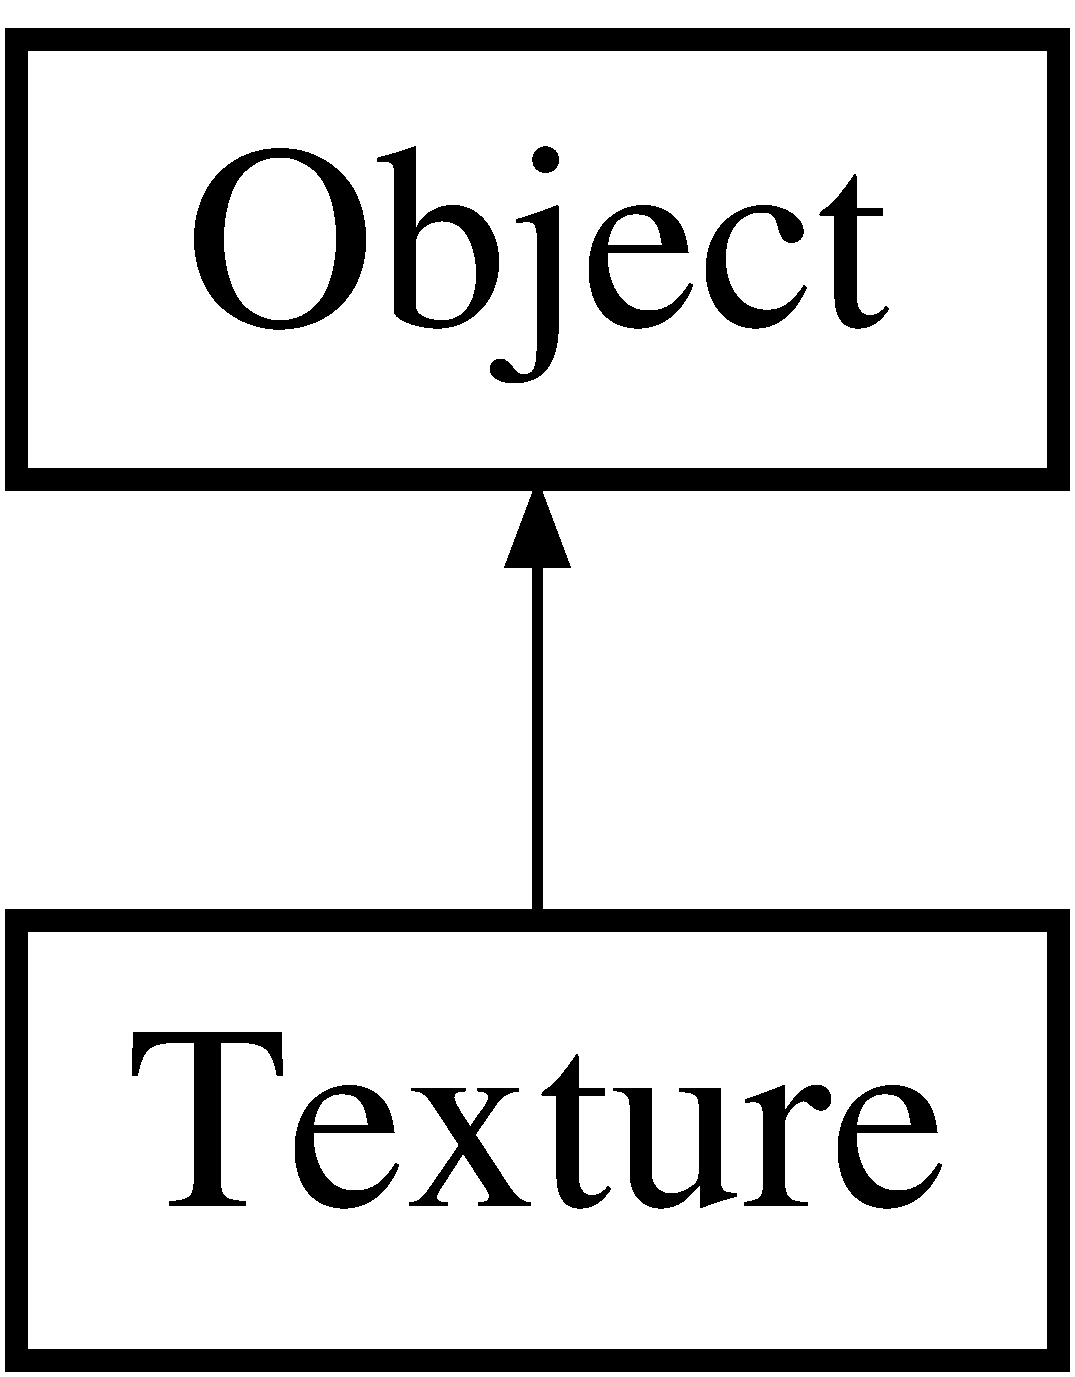
\includegraphics[height=2.000000cm]{class_texture}
\end{center}
\end{figure}
\subsection*{Public Member Functions}
\begin{DoxyCompactItemize}
\item 
\hyperlink{class_texture_af2a4c84d1c98677ce680586bc0fb4bb3}{Texture} (char $\ast$texture\+File\+Name=\char`\"{}\textbackslash{}0\char`\"{})
\begin{DoxyCompactList}\small\item\em Constructors. \end{DoxyCompactList}\item 
void \hyperlink{class_texture_ae4c6a5ee970eb169801555a2a0ca304c}{Init} (char $\ast$texture\+File\+Name)
\item 
virtual \hyperlink{class_texture_a09c4bcb7462f64c1d20fa69dba3cee8a}{$\sim$\+Texture} ()
\begin{DoxyCompactList}\small\item\em Destructor. \end{DoxyCompactList}\item 
void \hyperlink{class_texture_ae89d96eb1e3d905d37e64694628ec75a}{Fill\+Texture} (unsigned char $\ast$pix)
\begin{DoxyCompactList}\small\item\em Functions. \end{DoxyCompactList}\item 
void \hyperlink{class_texture_a7197223117d32c918ddfcd59d803a92e}{Load\+Texture} (char $\ast$texture\+File\+Name)
\item 
unsigned char $\ast$ \hyperlink{class_texture_a000d60714e60b703dd3f189e515c89a5}{Load\+Texture\+D\+DS} (O\+V\+R\+::\+File $\ast$file, int \&buff\+Size)
\item 
I\+D3\+D11\+Shader\+Resource\+View $\ast$\& \hyperlink{class_texture_a15710fdbf218bc437795d82b7d43d895}{Get\+Dx\+Shader\+Resource\+View} ()
\begin{DoxyCompactList}\small\item\em Getters. \end{DoxyCompactList}\item 
I\+D3\+D11\+Texture2D $\ast$ \hyperlink{class_texture_a2f7fb3841e9dcbbf8caf9ef3517b8c02}{Get\+Dx\+Texture} ()
\item 
I\+D3\+D11\+Render\+Target\+View $\ast$ \hyperlink{class_texture_ae9ff50740ff4ab8f9d4c19fd147d3bd2}{Get\+Dx\+Texture\+Render\+Target\+View} ()
\item 
int \hyperlink{class_texture_acc9f29e15f13b697f91779e2f87597b5}{Get\+Mipmap\+Levels} ()
\item 
int \hyperlink{class_texture_aa77eaaed00df44c7d9786d9a84e6a8c2}{Get\+Size\+Height} ()
\item 
int \hyperlink{class_texture_a1549f86a0410d3ea207fd991224eb45c}{Get\+Size\+Width} ()
\end{DoxyCompactItemize}
\subsection*{Protected Attributes}
\begin{DoxyCompactItemize}
\item 
O\+V\+R\+::\+Sys\+File $\ast$ \hyperlink{class_texture_aad71ad1112c80f067b0655c30cfa6e31}{my\+Texture\+File}
\item 
I\+D3\+D11\+Texture2D $\ast$ \hyperlink{class_texture_a162499ea3d2ad2f86fb94d0cc73b643c}{my\+Dx\+Texture}
\item 
I\+D3\+D11\+Shader\+Resource\+View $\ast$ \hyperlink{class_texture_ad6652783cd9346e82bd8159bfcad0d14}{my\+Dx\+Shader\+Resource\+View}
\item 
I\+D3\+D11\+Render\+Target\+View $\ast$ \hyperlink{class_texture_aafe1ab7239473c5acffbc14a5043ba3a}{my\+Dx\+Texture\+Render\+Target\+View}
\item 
unsigned char $\ast$ \hyperlink{class_texture_a0a158fa0c123a4ee1ac762a9708142f3}{my\+Pixel\+Buffer}
\item 
int \hyperlink{class_texture_abfb0ad95408fbefd68bafbaada18483c}{my\+Size\+Width}
\item 
int \hyperlink{class_texture_a83942c4f554c8af7884c31baf3a81b6e}{my\+Size\+Height}
\item 
int \hyperlink{class_texture_a350a5ae95df396fb43a75f023ff81e6e}{my\+Mipmap\+Levels}
\end{DoxyCompactItemize}
\subsection*{Additional Inherited Members}


\subsection{Constructor \& Destructor Documentation}
\index{Texture@{Texture}!Texture@{Texture}}
\index{Texture@{Texture}!Texture@{Texture}}
\subsubsection[{\texorpdfstring{Texture(char $\ast$texture\+File\+Name=""\textbackslash{}0"")}{Texture(char *textureFileName="\textbackslash{}0")}}]{\setlength{\rightskip}{0pt plus 5cm}Texture\+::\+Texture (
\begin{DoxyParamCaption}
\item[{char $\ast$}]{texture\+File\+Name = {\ttfamily \char`\"{}\textbackslash{}0\char`\"{}}}
\end{DoxyParamCaption}
)}\hypertarget{class_texture_af2a4c84d1c98677ce680586bc0fb4bb3}{}\label{class_texture_af2a4c84d1c98677ce680586bc0fb4bb3}


Constructors. 

Constructor, calls \hyperlink{class_texture_a7197223117d32c918ddfcd59d803a92e}{Load\+Texture()}.

\begin{DoxyAuthor}{Author}
Katianie 
\end{DoxyAuthor}
\begin{DoxyDate}{Date}
7/4/2016
\end{DoxyDate}

\begin{DoxyParams}[1]{Parameters}
\mbox{\tt in}  & {\em texture\+File\+Name} & The file name of the texture to load. \\
\hline
\end{DoxyParams}
\index{Texture@{Texture}!````~Texture@{$\sim$\+Texture}}
\index{````~Texture@{$\sim$\+Texture}!Texture@{Texture}}
\subsubsection[{\texorpdfstring{$\sim$\+Texture()}{~Texture()}}]{\setlength{\rightskip}{0pt plus 5cm}Texture\+::$\sim$\+Texture (
\begin{DoxyParamCaption}
{}
\end{DoxyParamCaption}
)\hspace{0.3cm}{\ttfamily [virtual]}}\hypertarget{class_texture_a09c4bcb7462f64c1d20fa69dba3cee8a}{}\label{class_texture_a09c4bcb7462f64c1d20fa69dba3cee8a}


Destructor. 

Destructor.

\begin{DoxyAuthor}{Author}
Katianie 
\end{DoxyAuthor}
\begin{DoxyDate}{Date}
7/4/2016 
\end{DoxyDate}


\subsection{Member Function Documentation}
\index{Texture@{Texture}!Fill\+Texture@{Fill\+Texture}}
\index{Fill\+Texture@{Fill\+Texture}!Texture@{Texture}}
\subsubsection[{\texorpdfstring{Fill\+Texture(unsigned char $\ast$pix)}{FillTexture(unsigned char *pix)}}]{\setlength{\rightskip}{0pt plus 5cm}void Texture\+::\+Fill\+Texture (
\begin{DoxyParamCaption}
\item[{unsigned char $\ast$}]{pix}
\end{DoxyParamCaption}
)}\hypertarget{class_texture_ae89d96eb1e3d905d37e64694628ec75a}{}\label{class_texture_ae89d96eb1e3d905d37e64694628ec75a}


Functions. 

Updates texture with the specified pixel buffer.

\begin{DoxyAuthor}{Author}
Katianie 
\end{DoxyAuthor}
\begin{DoxyDate}{Date}
7/4/2016
\end{DoxyDate}

\begin{DoxyParams}[1]{Parameters}
\mbox{\tt in,out}  & {\em The} & pixel buffer. \\
\hline
\end{DoxyParams}
\index{Texture@{Texture}!Get\+Dx\+Shader\+Resource\+View@{Get\+Dx\+Shader\+Resource\+View}}
\index{Get\+Dx\+Shader\+Resource\+View@{Get\+Dx\+Shader\+Resource\+View}!Texture@{Texture}}
\subsubsection[{\texorpdfstring{Get\+Dx\+Shader\+Resource\+View()}{GetDxShaderResourceView()}}]{\setlength{\rightskip}{0pt plus 5cm}I\+D3\+D11\+Shader\+Resource\+View $\ast$\& Texture\+::\+Get\+Dx\+Shader\+Resource\+View (
\begin{DoxyParamCaption}
{}
\end{DoxyParamCaption}
)}\hypertarget{class_texture_a15710fdbf218bc437795d82b7d43d895}{}\label{class_texture_a15710fdbf218bc437795d82b7d43d895}


Getters. 

Gets the DX Shader Resource View.

\begin{DoxyAuthor}{Author}
Katianie 
\end{DoxyAuthor}
\begin{DoxyDate}{Date}
7/4/2016
\end{DoxyDate}
\begin{DoxyReturn}{Returns}
The DX Shader Resource View. 
\end{DoxyReturn}
\index{Texture@{Texture}!Get\+Dx\+Texture@{Get\+Dx\+Texture}}
\index{Get\+Dx\+Texture@{Get\+Dx\+Texture}!Texture@{Texture}}
\subsubsection[{\texorpdfstring{Get\+Dx\+Texture()}{GetDxTexture()}}]{\setlength{\rightskip}{0pt plus 5cm}I\+D3\+D11\+Texture2D $\ast$ Texture\+::\+Get\+Dx\+Texture (
\begin{DoxyParamCaption}
{}
\end{DoxyParamCaption}
)}\hypertarget{class_texture_a2f7fb3841e9dcbbf8caf9ef3517b8c02}{}\label{class_texture_a2f7fb3841e9dcbbf8caf9ef3517b8c02}
Gets the DX \hyperlink{class_texture}{Texture}.

\begin{DoxyAuthor}{Author}
Katianie 
\end{DoxyAuthor}
\begin{DoxyDate}{Date}
7/4/2016
\end{DoxyDate}
\begin{DoxyReturn}{Returns}
The DX \hyperlink{class_texture}{Texture}. 
\end{DoxyReturn}
\index{Texture@{Texture}!Get\+Dx\+Texture\+Render\+Target\+View@{Get\+Dx\+Texture\+Render\+Target\+View}}
\index{Get\+Dx\+Texture\+Render\+Target\+View@{Get\+Dx\+Texture\+Render\+Target\+View}!Texture@{Texture}}
\subsubsection[{\texorpdfstring{Get\+Dx\+Texture\+Render\+Target\+View()}{GetDxTextureRenderTargetView()}}]{\setlength{\rightskip}{0pt plus 5cm}I\+D3\+D11\+Render\+Target\+View $\ast$ Texture\+::\+Get\+Dx\+Texture\+Render\+Target\+View (
\begin{DoxyParamCaption}
{}
\end{DoxyParamCaption}
)}\hypertarget{class_texture_ae9ff50740ff4ab8f9d4c19fd147d3bd2}{}\label{class_texture_ae9ff50740ff4ab8f9d4c19fd147d3bd2}
Gets the DX \hyperlink{class_texture}{Texture} Render Target View.

\begin{DoxyAuthor}{Author}
Katianie 
\end{DoxyAuthor}
\begin{DoxyDate}{Date}
7/4/2016
\end{DoxyDate}
\begin{DoxyReturn}{Returns}
The DX \hyperlink{class_texture}{Texture} Render Target View. 
\end{DoxyReturn}
\index{Texture@{Texture}!Get\+Mipmap\+Levels@{Get\+Mipmap\+Levels}}
\index{Get\+Mipmap\+Levels@{Get\+Mipmap\+Levels}!Texture@{Texture}}
\subsubsection[{\texorpdfstring{Get\+Mipmap\+Levels()}{GetMipmapLevels()}}]{\setlength{\rightskip}{0pt plus 5cm}int Texture\+::\+Get\+Mipmap\+Levels (
\begin{DoxyParamCaption}
{}
\end{DoxyParamCaption}
)}\hypertarget{class_texture_acc9f29e15f13b697f91779e2f87597b5}{}\label{class_texture_acc9f29e15f13b697f91779e2f87597b5}
Gets the Mipmap levels of the texture.

\begin{DoxyAuthor}{Author}
Katianie 
\end{DoxyAuthor}
\begin{DoxyDate}{Date}
7/4/2016
\end{DoxyDate}
\begin{DoxyReturn}{Returns}
The Mipmap levels of the texture. 
\end{DoxyReturn}
\index{Texture@{Texture}!Get\+Size\+Height@{Get\+Size\+Height}}
\index{Get\+Size\+Height@{Get\+Size\+Height}!Texture@{Texture}}
\subsubsection[{\texorpdfstring{Get\+Size\+Height()}{GetSizeHeight()}}]{\setlength{\rightskip}{0pt plus 5cm}int Texture\+::\+Get\+Size\+Height (
\begin{DoxyParamCaption}
{}
\end{DoxyParamCaption}
)}\hypertarget{class_texture_aa77eaaed00df44c7d9786d9a84e6a8c2}{}\label{class_texture_aa77eaaed00df44c7d9786d9a84e6a8c2}
Gets the height of the \hyperlink{class_texture}{Texture}.

\begin{DoxyAuthor}{Author}
Katianie 
\end{DoxyAuthor}
\begin{DoxyDate}{Date}
7/4/2016
\end{DoxyDate}
\begin{DoxyReturn}{Returns}
The size height. 
\end{DoxyReturn}
\index{Texture@{Texture}!Get\+Size\+Width@{Get\+Size\+Width}}
\index{Get\+Size\+Width@{Get\+Size\+Width}!Texture@{Texture}}
\subsubsection[{\texorpdfstring{Get\+Size\+Width()}{GetSizeWidth()}}]{\setlength{\rightskip}{0pt plus 5cm}int Texture\+::\+Get\+Size\+Width (
\begin{DoxyParamCaption}
{}
\end{DoxyParamCaption}
)}\hypertarget{class_texture_a1549f86a0410d3ea207fd991224eb45c}{}\label{class_texture_a1549f86a0410d3ea207fd991224eb45c}
Gets the width of the \hyperlink{class_texture}{Texture}.

\begin{DoxyAuthor}{Author}
Katianie 
\end{DoxyAuthor}
\begin{DoxyDate}{Date}
7/4/2016
\end{DoxyDate}
\begin{DoxyReturn}{Returns}
The width of the \hyperlink{class_texture}{Texture}. 
\end{DoxyReturn}
\index{Texture@{Texture}!Init@{Init}}
\index{Init@{Init}!Texture@{Texture}}
\subsubsection[{\texorpdfstring{Init(char $\ast$texture\+File\+Name)}{Init(char *textureFileName)}}]{\setlength{\rightskip}{0pt plus 5cm}void Texture\+::\+Init (
\begin{DoxyParamCaption}
\item[{char $\ast$}]{texture\+File\+Name}
\end{DoxyParamCaption}
)}\hypertarget{class_texture_ae4c6a5ee970eb169801555a2a0ca304c}{}\label{class_texture_ae4c6a5ee970eb169801555a2a0ca304c}
Call \hyperlink{class_texture_ae4c6a5ee970eb169801555a2a0ca304c}{Init()} after we load the texture so we know the width, height, etc. See \hyperlink{class_texture_a7197223117d32c918ddfcd59d803a92e}{Load\+Texture()}.

\begin{DoxyAuthor}{Author}
Katianie 
\end{DoxyAuthor}
\begin{DoxyDate}{Date}
7/4/2016
\end{DoxyDate}

\begin{DoxyParams}[1]{Parameters}
\mbox{\tt in,out}  & {\em texture\+File\+Name} & If non-\/null, filename of the texture file. \\
\hline
\end{DoxyParams}
\index{Texture@{Texture}!Load\+Texture@{Load\+Texture}}
\index{Load\+Texture@{Load\+Texture}!Texture@{Texture}}
\subsubsection[{\texorpdfstring{Load\+Texture(char $\ast$texture\+File\+Name)}{LoadTexture(char *textureFileName)}}]{\setlength{\rightskip}{0pt plus 5cm}void Texture\+::\+Load\+Texture (
\begin{DoxyParamCaption}
\item[{char $\ast$}]{texture\+File\+Name}
\end{DoxyParamCaption}
)}\hypertarget{class_texture_a7197223117d32c918ddfcd59d803a92e}{}\label{class_texture_a7197223117d32c918ddfcd59d803a92e}
Loads a texture from the specified file name.

\begin{DoxyAuthor}{Author}
Katianie 
\end{DoxyAuthor}
\begin{DoxyDate}{Date}
7/4/2016
\end{DoxyDate}

\begin{DoxyParams}[1]{Parameters}
\mbox{\tt in}  & {\em texture\+File\+Name} & The filename of the texture file. \\
\hline
\end{DoxyParams}
\index{Texture@{Texture}!Load\+Texture\+D\+DS@{Load\+Texture\+D\+DS}}
\index{Load\+Texture\+D\+DS@{Load\+Texture\+D\+DS}!Texture@{Texture}}
\subsubsection[{\texorpdfstring{Load\+Texture\+D\+D\+S(\+O\+V\+R\+::\+File $\ast$file, int \&buff\+Size)}{LoadTextureDDS(OVR::File *file, int &buffSize)}}]{\setlength{\rightskip}{0pt plus 5cm}unsigned char $\ast$ Texture\+::\+Load\+Texture\+D\+DS (
\begin{DoxyParamCaption}
\item[{O\+V\+R\+::\+File $\ast$}]{file, }
\item[{int \&}]{buff\+Size}
\end{DoxyParamCaption}
)}\hypertarget{class_texture_a000d60714e60b703dd3f189e515c89a5}{}\label{class_texture_a000d60714e60b703dd3f189e515c89a5}
Loads the file and allocates the texture pixel buffer.

\begin{DoxyAuthor}{Author}
Katianie 
\end{DoxyAuthor}
\begin{DoxyDate}{Date}
7/4/2016
\end{DoxyDate}

\begin{DoxyParams}[1]{Parameters}
\mbox{\tt in}  & {\em file} & The file to load. \\
\hline
\mbox{\tt in}  & {\em buff\+Size} & Size of the buffer.\\
\hline
\end{DoxyParams}
\begin{DoxyReturn}{Returns}
The texture pixel buffer. 
\end{DoxyReturn}


\subsection{Member Data Documentation}
\index{Texture@{Texture}!my\+Dx\+Shader\+Resource\+View@{my\+Dx\+Shader\+Resource\+View}}
\index{my\+Dx\+Shader\+Resource\+View@{my\+Dx\+Shader\+Resource\+View}!Texture@{Texture}}
\subsubsection[{\texorpdfstring{my\+Dx\+Shader\+Resource\+View}{myDxShaderResourceView}}]{\setlength{\rightskip}{0pt plus 5cm}I\+D3\+D11\+Shader\+Resource\+View$\ast$ Texture\+::my\+Dx\+Shader\+Resource\+View\hspace{0.3cm}{\ttfamily [protected]}}\hypertarget{class_texture_ad6652783cd9346e82bd8159bfcad0d14}{}\label{class_texture_ad6652783cd9346e82bd8159bfcad0d14}
\index{Texture@{Texture}!my\+Dx\+Texture@{my\+Dx\+Texture}}
\index{my\+Dx\+Texture@{my\+Dx\+Texture}!Texture@{Texture}}
\subsubsection[{\texorpdfstring{my\+Dx\+Texture}{myDxTexture}}]{\setlength{\rightskip}{0pt plus 5cm}I\+D3\+D11\+Texture2D$\ast$ Texture\+::my\+Dx\+Texture\hspace{0.3cm}{\ttfamily [protected]}}\hypertarget{class_texture_a162499ea3d2ad2f86fb94d0cc73b643c}{}\label{class_texture_a162499ea3d2ad2f86fb94d0cc73b643c}
\index{Texture@{Texture}!my\+Dx\+Texture\+Render\+Target\+View@{my\+Dx\+Texture\+Render\+Target\+View}}
\index{my\+Dx\+Texture\+Render\+Target\+View@{my\+Dx\+Texture\+Render\+Target\+View}!Texture@{Texture}}
\subsubsection[{\texorpdfstring{my\+Dx\+Texture\+Render\+Target\+View}{myDxTextureRenderTargetView}}]{\setlength{\rightskip}{0pt plus 5cm}I\+D3\+D11\+Render\+Target\+View$\ast$ Texture\+::my\+Dx\+Texture\+Render\+Target\+View\hspace{0.3cm}{\ttfamily [protected]}}\hypertarget{class_texture_aafe1ab7239473c5acffbc14a5043ba3a}{}\label{class_texture_aafe1ab7239473c5acffbc14a5043ba3a}
\index{Texture@{Texture}!my\+Mipmap\+Levels@{my\+Mipmap\+Levels}}
\index{my\+Mipmap\+Levels@{my\+Mipmap\+Levels}!Texture@{Texture}}
\subsubsection[{\texorpdfstring{my\+Mipmap\+Levels}{myMipmapLevels}}]{\setlength{\rightskip}{0pt plus 5cm}int Texture\+::my\+Mipmap\+Levels\hspace{0.3cm}{\ttfamily [protected]}}\hypertarget{class_texture_a350a5ae95df396fb43a75f023ff81e6e}{}\label{class_texture_a350a5ae95df396fb43a75f023ff81e6e}
\index{Texture@{Texture}!my\+Pixel\+Buffer@{my\+Pixel\+Buffer}}
\index{my\+Pixel\+Buffer@{my\+Pixel\+Buffer}!Texture@{Texture}}
\subsubsection[{\texorpdfstring{my\+Pixel\+Buffer}{myPixelBuffer}}]{\setlength{\rightskip}{0pt plus 5cm}unsigned char$\ast$ Texture\+::my\+Pixel\+Buffer\hspace{0.3cm}{\ttfamily [protected]}}\hypertarget{class_texture_a0a158fa0c123a4ee1ac762a9708142f3}{}\label{class_texture_a0a158fa0c123a4ee1ac762a9708142f3}
\index{Texture@{Texture}!my\+Size\+Height@{my\+Size\+Height}}
\index{my\+Size\+Height@{my\+Size\+Height}!Texture@{Texture}}
\subsubsection[{\texorpdfstring{my\+Size\+Height}{mySizeHeight}}]{\setlength{\rightskip}{0pt plus 5cm}int Texture\+::my\+Size\+Height\hspace{0.3cm}{\ttfamily [protected]}}\hypertarget{class_texture_a83942c4f554c8af7884c31baf3a81b6e}{}\label{class_texture_a83942c4f554c8af7884c31baf3a81b6e}
\index{Texture@{Texture}!my\+Size\+Width@{my\+Size\+Width}}
\index{my\+Size\+Width@{my\+Size\+Width}!Texture@{Texture}}
\subsubsection[{\texorpdfstring{my\+Size\+Width}{mySizeWidth}}]{\setlength{\rightskip}{0pt plus 5cm}int Texture\+::my\+Size\+Width\hspace{0.3cm}{\ttfamily [protected]}}\hypertarget{class_texture_abfb0ad95408fbefd68bafbaada18483c}{}\label{class_texture_abfb0ad95408fbefd68bafbaada18483c}
\index{Texture@{Texture}!my\+Texture\+File@{my\+Texture\+File}}
\index{my\+Texture\+File@{my\+Texture\+File}!Texture@{Texture}}
\subsubsection[{\texorpdfstring{my\+Texture\+File}{myTextureFile}}]{\setlength{\rightskip}{0pt plus 5cm}O\+V\+R\+::\+Sys\+File$\ast$ Texture\+::my\+Texture\+File\hspace{0.3cm}{\ttfamily [protected]}}\hypertarget{class_texture_aad71ad1112c80f067b0655c30cfa6e31}{}\label{class_texture_aad71ad1112c80f067b0655c30cfa6e31}


The documentation for this class was generated from the following files\+:\begin{DoxyCompactItemize}
\item 
Samples/\+Oculus\+Room\+Tiny\+\_\+\+Advanced/\+Common/\+Headers/\hyperlink{_texture_8h}{Texture.\+h}\item 
Samples/\+Oculus\+Room\+Tiny\+\_\+\+Advanced/\+Common/\+Implementations/\hyperlink{_texture_8cpp}{Texture.\+cpp}\end{DoxyCompactItemize}

\hypertarget{class_triangle_set}{}\section{Triangle\+Set Class Reference}
\label{class_triangle_set}\index{Triangle\+Set@{Triangle\+Set}}


{\ttfamily \#include $<$Triangle\+Set.\+h$>$}

Inheritance diagram for Triangle\+Set\+:\begin{figure}[H]
\begin{center}
\leavevmode
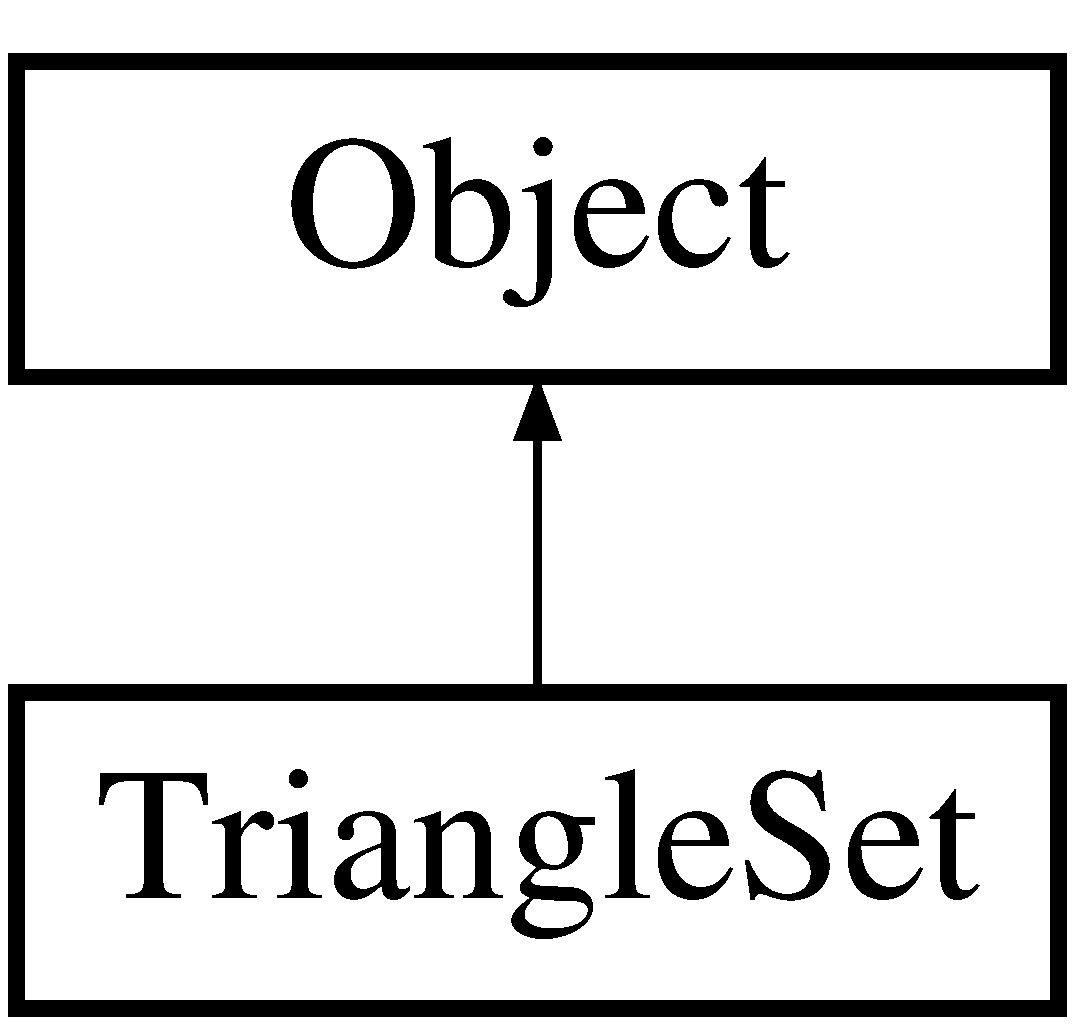
\includegraphics[height=2.000000cm]{class_triangle_set}
\end{center}
\end{figure}
\subsection*{Public Member Functions}
\begin{DoxyCompactItemize}
\item 
\hyperlink{class_triangle_set_af476769901923751b75c28b3fb405287}{Triangle\+Set} (int max\+Triangles=M\+A\+X\+\_\+\+T\+R\+I\+A\+N\+G\+L\+ES, short $\ast$indices=N\+U\+LL, \hyperlink{class_vertex}{Vertex} $\ast$vertices=N\+U\+LL)
\begin{DoxyCompactList}\small\item\em Constructor. \end{DoxyCompactList}\item 
\hyperlink{class_triangle_set_a04eaa39a57ece1a96c853eed01d54b88}{$\sim$\+Triangle\+Set} ()
\begin{DoxyCompactList}\small\item\em Destructor. \end{DoxyCompactList}\item 
void \hyperlink{class_triangle_set_a272ae3bd26d941b6e1a902ef7333bbb1}{Add\+Quad} (\hyperlink{class_vertex}{Vertex} v0, \hyperlink{class_vertex}{Vertex} v1, \hyperlink{class_vertex}{Vertex} v2, \hyperlink{class_vertex}{Vertex} v3)
\begin{DoxyCompactList}\small\item\em Functions. \end{DoxyCompactList}\item 
void \hyperlink{class_triangle_set_a2207831afe53a8bb3298d661391a1418}{Add\+Triangle} (\hyperlink{class_vertex}{Vertex} v0, \hyperlink{class_vertex}{Vertex} v1, \hyperlink{class_vertex}{Vertex} v2, bool generate\+Indices=true)
\item 
void \hyperlink{class_triangle_set_a3482e212da7004ff55c6d087047904db}{Create\+Panoramic} (int angle\+Of\+Panoramic\+Image, float radius, float height)
\item 
void \hyperlink{class_triangle_set_ac5bc6b68fa1118e12900f0d2638e2b5a}{Create\+Sphere} (float radius)
\item 
void \hyperlink{class_triangle_set_a95c9d8f500a7facd53d2af30cd7104be}{Load\+Geomerty} (vector$<$ Vertex\+Position\+Normal\+Texture $>$ vertices, vector$<$ uint16\+\_\+t $>$ indices)
\item 
short $\ast$ \hyperlink{class_triangle_set_af7318e823cda708835e3b47ce83bae23}{Get\+Indices} ()
\begin{DoxyCompactList}\small\item\em Getters. \end{DoxyCompactList}\item 
int \hyperlink{class_triangle_set_a23da7e4699bc2e22664c000fac27a962}{Get\+Max\+Buffer\+Size} ()
\item 
int \hyperlink{class_triangle_set_a8cda203213cce0f4edb87226daf1ef1e}{Get\+Num\+Indices} ()
\item 
int \hyperlink{class_triangle_set_ae4999e314948b3fe30ade2299a5b815d}{Get\+Num\+Vertices} ()
\item 
\hyperlink{class_vertex}{Vertex} $\ast$ \hyperlink{class_triangle_set_affe9e0e2d4f07f6b728e9d51e21a6087}{Get\+Vertices} ()
\end{DoxyCompactItemize}
\subsection*{Protected Attributes}
\begin{DoxyCompactItemize}
\item 
int \hyperlink{class_triangle_set_a0c4ae28e04e40ca53e37ef2579069f92}{my\+Num\+Indices}
\item 
int \hyperlink{class_triangle_set_aaa4eb472d41e4d1a3c0e4ef7524cacfa}{my\+Num\+Vertices}
\item 
int \hyperlink{class_triangle_set_a5438cf58a0180a411634bba22d0bc829}{my\+Max\+Buffer\+Size}
\item 
short $\ast$ \hyperlink{class_triangle_set_a3685b9957ee6383120d5b38407cb731d}{my\+Indices}
\item 
\hyperlink{class_vertex}{Vertex} $\ast$ \hyperlink{class_triangle_set_ae05f53594858e811f4aa0d866b9e9665}{my\+Vertices}
\end{DoxyCompactItemize}
\subsection*{Additional Inherited Members}


\subsection{Constructor \& Destructor Documentation}
\index{Triangle\+Set@{Triangle\+Set}!Triangle\+Set@{Triangle\+Set}}
\index{Triangle\+Set@{Triangle\+Set}!Triangle\+Set@{Triangle\+Set}}
\subsubsection[{\texorpdfstring{Triangle\+Set(int max\+Triangles=\+M\+A\+X\+\_\+\+T\+R\+I\+A\+N\+G\+L\+E\+S, short $\ast$indices=\+N\+U\+L\+L, Vertex $\ast$vertices=\+N\+U\+L\+L)}{TriangleSet(int maxTriangles=MAX_TRIANGLES, short *indices=NULL, Vertex *vertices=NULL)}}]{\setlength{\rightskip}{0pt plus 5cm}Triangle\+Set\+::\+Triangle\+Set (
\begin{DoxyParamCaption}
\item[{int}]{max\+Triangles = {\ttfamily MAX\+\_\+TRIANGLES}, }
\item[{short $\ast$}]{indices = {\ttfamily NULL}, }
\item[{{\bf Vertex} $\ast$}]{vertices = {\ttfamily NULL}}
\end{DoxyParamCaption}
)}\hypertarget{class_triangle_set_af476769901923751b75c28b3fb405287}{}\label{class_triangle_set_af476769901923751b75c28b3fb405287}


Constructor. 

Constructor, allocates a vertex and index buffer.

\begin{DoxyAuthor}{Author}
Katianie 
\end{DoxyAuthor}
\begin{DoxyDate}{Date}
7/4/2016
\end{DoxyDate}

\begin{DoxyParams}[1]{Parameters}
 & {\em max\+Triangles} & The maximum number of triangles to allow. \\
\hline
\mbox{\tt in,out}  & {\em indices} & An index buffer, if null, its created here. \\
\hline
\mbox{\tt in,out}  & {\em vertices} & A vertex buffer, if null, its created here. \\
\hline
\end{DoxyParams}
\index{Triangle\+Set@{Triangle\+Set}!````~Triangle\+Set@{$\sim$\+Triangle\+Set}}
\index{````~Triangle\+Set@{$\sim$\+Triangle\+Set}!Triangle\+Set@{Triangle\+Set}}
\subsubsection[{\texorpdfstring{$\sim$\+Triangle\+Set()}{~TriangleSet()}}]{\setlength{\rightskip}{0pt plus 5cm}Triangle\+Set\+::$\sim$\+Triangle\+Set (
\begin{DoxyParamCaption}
{}
\end{DoxyParamCaption}
)}\hypertarget{class_triangle_set_a04eaa39a57ece1a96c853eed01d54b88}{}\label{class_triangle_set_a04eaa39a57ece1a96c853eed01d54b88}


Destructor. 

Destructor, deletes and cleans up index and vertex buffer.

\begin{DoxyAuthor}{Author}
Katianie 
\end{DoxyAuthor}
\begin{DoxyDate}{Date}
7/4/2016 
\end{DoxyDate}


\subsection{Member Function Documentation}
\index{Triangle\+Set@{Triangle\+Set}!Add\+Quad@{Add\+Quad}}
\index{Add\+Quad@{Add\+Quad}!Triangle\+Set@{Triangle\+Set}}
\subsubsection[{\texorpdfstring{Add\+Quad(\+Vertex v0, Vertex v1, Vertex v2, Vertex v3)}{AddQuad(Vertex v0, Vertex v1, Vertex v2, Vertex v3)}}]{\setlength{\rightskip}{0pt plus 5cm}void Triangle\+Set\+::\+Add\+Quad (
\begin{DoxyParamCaption}
\item[{{\bf Vertex}}]{v0, }
\item[{{\bf Vertex}}]{v1, }
\item[{{\bf Vertex}}]{v2, }
\item[{{\bf Vertex}}]{v3}
\end{DoxyParamCaption}
)}\hypertarget{class_triangle_set_a272ae3bd26d941b6e1a902ef7333bbb1}{}\label{class_triangle_set_a272ae3bd26d941b6e1a902ef7333bbb1}


Functions. 

Creates a square using triangles.

\begin{DoxyAuthor}{Author}
Katianie 
\end{DoxyAuthor}
\begin{DoxyDate}{Date}
7/4/2016
\end{DoxyDate}

\begin{DoxyParams}{Parameters}
{\em v0} & The first vertex of the square. \\
\hline
{\em v1} & The second vertex of the square. \\
\hline
{\em v2} & The third vertex of the square. \\
\hline
{\em v3} & The fourth vertex of the square. \\
\hline
\end{DoxyParams}
\index{Triangle\+Set@{Triangle\+Set}!Add\+Triangle@{Add\+Triangle}}
\index{Add\+Triangle@{Add\+Triangle}!Triangle\+Set@{Triangle\+Set}}
\subsubsection[{\texorpdfstring{Add\+Triangle(\+Vertex v0, Vertex v1, Vertex v2, bool generate\+Indices=true)}{AddTriangle(Vertex v0, Vertex v1, Vertex v2, bool generateIndices=true)}}]{\setlength{\rightskip}{0pt plus 5cm}void Triangle\+Set\+::\+Add\+Triangle (
\begin{DoxyParamCaption}
\item[{{\bf Vertex}}]{v0, }
\item[{{\bf Vertex}}]{v1, }
\item[{{\bf Vertex}}]{v2, }
\item[{bool}]{generate\+Indices = {\ttfamily true}}
\end{DoxyParamCaption}
)}\hypertarget{class_triangle_set_a2207831afe53a8bb3298d661391a1418}{}\label{class_triangle_set_a2207831afe53a8bb3298d661391a1418}
Adds a single triangle to the vertex and index buffer.

\begin{DoxyAuthor}{Author}
Katianie 
\end{DoxyAuthor}
\begin{DoxyDate}{Date}
7/4/2016
\end{DoxyDate}

\begin{DoxyParams}{Parameters}
{\em v0} & The first vertex. \\
\hline
{\em v1} & The second \hyperlink{class_vertex}{Vertex}. \\
\hline
{\em v2} & The third \hyperlink{class_vertex}{Vertex}. \\
\hline
{\em generate\+Indices} & true to generate indices. \\
\hline
\end{DoxyParams}
\index{Triangle\+Set@{Triangle\+Set}!Create\+Panoramic@{Create\+Panoramic}}
\index{Create\+Panoramic@{Create\+Panoramic}!Triangle\+Set@{Triangle\+Set}}
\subsubsection[{\texorpdfstring{Create\+Panoramic(int angle\+Of\+Panoramic\+Image, float radius, float height)}{CreatePanoramic(int angleOfPanoramicImage, float radius, float height)}}]{\setlength{\rightskip}{0pt plus 5cm}void Triangle\+Set\+::\+Create\+Panoramic (
\begin{DoxyParamCaption}
\item[{int}]{angle\+Of\+Panoramic\+Image, }
\item[{float}]{radius, }
\item[{float}]{height}
\end{DoxyParamCaption}
)}\hypertarget{class_triangle_set_a3482e212da7004ff55c6d087047904db}{}\label{class_triangle_set_a3482e212da7004ff55c6d087047904db}
Creates the partial cylinder geometry used for 180, 270, and 360 views.

\begin{DoxyAuthor}{Author}
Katianie 
\end{DoxyAuthor}
\begin{DoxyDate}{Date}
7/4/2016
\end{DoxyDate}

\begin{DoxyParams}{Parameters}
{\em angle\+Of\+Panoramic\+Image} & The angle of panoramic image (180, 270, or 360). \\
\hline
{\em radius} & The radius of the partial cylinder. \\
\hline
{\em height} & The height of the partial cylinder. \\
\hline
\end{DoxyParams}
\index{Triangle\+Set@{Triangle\+Set}!Create\+Sphere@{Create\+Sphere}}
\index{Create\+Sphere@{Create\+Sphere}!Triangle\+Set@{Triangle\+Set}}
\subsubsection[{\texorpdfstring{Create\+Sphere(float radius)}{CreateSphere(float radius)}}]{\setlength{\rightskip}{0pt plus 5cm}void Triangle\+Set\+::\+Create\+Sphere (
\begin{DoxyParamCaption}
\item[{float}]{radius}
\end{DoxyParamCaption}
)}\hypertarget{class_triangle_set_ac5bc6b68fa1118e12900f0d2638e2b5a}{}\label{class_triangle_set_ac5bc6b68fa1118e12900f0d2638e2b5a}
Creates the sphere used for photosphere views.

\begin{DoxyAuthor}{Author}
Katianie 
\end{DoxyAuthor}
\begin{DoxyDate}{Date}
7/4/2016
\end{DoxyDate}

\begin{DoxyParams}{Parameters}
{\em radius} & The radius of the sphere. \\
\hline
\end{DoxyParams}
\index{Triangle\+Set@{Triangle\+Set}!Get\+Indices@{Get\+Indices}}
\index{Get\+Indices@{Get\+Indices}!Triangle\+Set@{Triangle\+Set}}
\subsubsection[{\texorpdfstring{Get\+Indices()}{GetIndices()}}]{\setlength{\rightskip}{0pt plus 5cm}short $\ast$ Triangle\+Set\+::\+Get\+Indices (
\begin{DoxyParamCaption}
{}
\end{DoxyParamCaption}
)}\hypertarget{class_triangle_set_af7318e823cda708835e3b47ce83bae23}{}\label{class_triangle_set_af7318e823cda708835e3b47ce83bae23}


Getters. 

Gets the index buffer.

\begin{DoxyAuthor}{Author}
Katianie 
\end{DoxyAuthor}
\begin{DoxyDate}{Date}
7/4/2016
\end{DoxyDate}
\begin{DoxyReturn}{Returns}
The index buffer. 
\end{DoxyReturn}
\index{Triangle\+Set@{Triangle\+Set}!Get\+Max\+Buffer\+Size@{Get\+Max\+Buffer\+Size}}
\index{Get\+Max\+Buffer\+Size@{Get\+Max\+Buffer\+Size}!Triangle\+Set@{Triangle\+Set}}
\subsubsection[{\texorpdfstring{Get\+Max\+Buffer\+Size()}{GetMaxBufferSize()}}]{\setlength{\rightskip}{0pt plus 5cm}int Triangle\+Set\+::\+Get\+Max\+Buffer\+Size (
\begin{DoxyParamCaption}
{}
\end{DoxyParamCaption}
)}\hypertarget{class_triangle_set_a23da7e4699bc2e22664c000fac27a962}{}\label{class_triangle_set_a23da7e4699bc2e22664c000fac27a962}
Gets maximum buffer size.

\begin{DoxyAuthor}{Author}
Katianie 
\end{DoxyAuthor}
\begin{DoxyDate}{Date}
7/4/2016
\end{DoxyDate}
\begin{DoxyReturn}{Returns}
The maximum buffer size. 
\end{DoxyReturn}
\index{Triangle\+Set@{Triangle\+Set}!Get\+Num\+Indices@{Get\+Num\+Indices}}
\index{Get\+Num\+Indices@{Get\+Num\+Indices}!Triangle\+Set@{Triangle\+Set}}
\subsubsection[{\texorpdfstring{Get\+Num\+Indices()}{GetNumIndices()}}]{\setlength{\rightskip}{0pt plus 5cm}int Triangle\+Set\+::\+Get\+Num\+Indices (
\begin{DoxyParamCaption}
{}
\end{DoxyParamCaption}
)}\hypertarget{class_triangle_set_a8cda203213cce0f4edb87226daf1ef1e}{}\label{class_triangle_set_a8cda203213cce0f4edb87226daf1ef1e}
Gets number indices.

\begin{DoxyAuthor}{Author}
Katianie 
\end{DoxyAuthor}
\begin{DoxyDate}{Date}
7/4/2016
\end{DoxyDate}
\begin{DoxyReturn}{Returns}
The number indices. 
\end{DoxyReturn}
\index{Triangle\+Set@{Triangle\+Set}!Get\+Num\+Vertices@{Get\+Num\+Vertices}}
\index{Get\+Num\+Vertices@{Get\+Num\+Vertices}!Triangle\+Set@{Triangle\+Set}}
\subsubsection[{\texorpdfstring{Get\+Num\+Vertices()}{GetNumVertices()}}]{\setlength{\rightskip}{0pt plus 5cm}int Triangle\+Set\+::\+Get\+Num\+Vertices (
\begin{DoxyParamCaption}
{}
\end{DoxyParamCaption}
)}\hypertarget{class_triangle_set_ae4999e314948b3fe30ade2299a5b815d}{}\label{class_triangle_set_ae4999e314948b3fe30ade2299a5b815d}
Gets number vertices.

\begin{DoxyAuthor}{Author}
Katianie 
\end{DoxyAuthor}
\begin{DoxyDate}{Date}
7/4/2016
\end{DoxyDate}
\begin{DoxyReturn}{Returns}
The number vertices. 
\end{DoxyReturn}
\index{Triangle\+Set@{Triangle\+Set}!Get\+Vertices@{Get\+Vertices}}
\index{Get\+Vertices@{Get\+Vertices}!Triangle\+Set@{Triangle\+Set}}
\subsubsection[{\texorpdfstring{Get\+Vertices()}{GetVertices()}}]{\setlength{\rightskip}{0pt plus 5cm}{\bf Vertex} $\ast$ Triangle\+Set\+::\+Get\+Vertices (
\begin{DoxyParamCaption}
{}
\end{DoxyParamCaption}
)}\hypertarget{class_triangle_set_affe9e0e2d4f07f6b728e9d51e21a6087}{}\label{class_triangle_set_affe9e0e2d4f07f6b728e9d51e21a6087}
Gets the vertex buffer.

\begin{DoxyAuthor}{Author}
Katianie 
\end{DoxyAuthor}
\begin{DoxyDate}{Date}
7/4/2016
\end{DoxyDate}
\begin{DoxyReturn}{Returns}
The vertex buffer. 
\end{DoxyReturn}
\index{Triangle\+Set@{Triangle\+Set}!Load\+Geomerty@{Load\+Geomerty}}
\index{Load\+Geomerty@{Load\+Geomerty}!Triangle\+Set@{Triangle\+Set}}
\subsubsection[{\texorpdfstring{Load\+Geomerty(vector$<$ Vertex\+Position\+Normal\+Texture $>$ vertices, vector$<$ uint16\+\_\+t $>$ indices)}{LoadGeomerty(vector< VertexPositionNormalTexture > vertices, vector< uint16_t > indices)}}]{\setlength{\rightskip}{0pt plus 5cm}void Triangle\+Set\+::\+Load\+Geomerty (
\begin{DoxyParamCaption}
\item[{vector$<$ Vertex\+Position\+Normal\+Texture $>$}]{vertices, }
\item[{vector$<$ uint16\+\_\+t $>$}]{indices}
\end{DoxyParamCaption}
)}\hypertarget{class_triangle_set_a95c9d8f500a7facd53d2af30cd7104be}{}\label{class_triangle_set_a95c9d8f500a7facd53d2af30cd7104be}
Takes in raw vertex and index buffers and creates the triangles of the model and assembles them.

\begin{DoxyAuthor}{Author}
Katianie 
\end{DoxyAuthor}
\begin{DoxyDate}{Date}
7/4/2016
\end{DoxyDate}

\begin{DoxyParams}{Parameters}
{\em vertices} & The vertices to load. \\
\hline
{\em indices} & The indices to load. \\
\hline
\end{DoxyParams}


\subsection{Member Data Documentation}
\index{Triangle\+Set@{Triangle\+Set}!my\+Indices@{my\+Indices}}
\index{my\+Indices@{my\+Indices}!Triangle\+Set@{Triangle\+Set}}
\subsubsection[{\texorpdfstring{my\+Indices}{myIndices}}]{\setlength{\rightskip}{0pt plus 5cm}short$\ast$ Triangle\+Set\+::my\+Indices\hspace{0.3cm}{\ttfamily [protected]}}\hypertarget{class_triangle_set_a3685b9957ee6383120d5b38407cb731d}{}\label{class_triangle_set_a3685b9957ee6383120d5b38407cb731d}
\index{Triangle\+Set@{Triangle\+Set}!my\+Max\+Buffer\+Size@{my\+Max\+Buffer\+Size}}
\index{my\+Max\+Buffer\+Size@{my\+Max\+Buffer\+Size}!Triangle\+Set@{Triangle\+Set}}
\subsubsection[{\texorpdfstring{my\+Max\+Buffer\+Size}{myMaxBufferSize}}]{\setlength{\rightskip}{0pt plus 5cm}int Triangle\+Set\+::my\+Max\+Buffer\+Size\hspace{0.3cm}{\ttfamily [protected]}}\hypertarget{class_triangle_set_a5438cf58a0180a411634bba22d0bc829}{}\label{class_triangle_set_a5438cf58a0180a411634bba22d0bc829}
\index{Triangle\+Set@{Triangle\+Set}!my\+Num\+Indices@{my\+Num\+Indices}}
\index{my\+Num\+Indices@{my\+Num\+Indices}!Triangle\+Set@{Triangle\+Set}}
\subsubsection[{\texorpdfstring{my\+Num\+Indices}{myNumIndices}}]{\setlength{\rightskip}{0pt plus 5cm}int Triangle\+Set\+::my\+Num\+Indices\hspace{0.3cm}{\ttfamily [protected]}}\hypertarget{class_triangle_set_a0c4ae28e04e40ca53e37ef2579069f92}{}\label{class_triangle_set_a0c4ae28e04e40ca53e37ef2579069f92}
\index{Triangle\+Set@{Triangle\+Set}!my\+Num\+Vertices@{my\+Num\+Vertices}}
\index{my\+Num\+Vertices@{my\+Num\+Vertices}!Triangle\+Set@{Triangle\+Set}}
\subsubsection[{\texorpdfstring{my\+Num\+Vertices}{myNumVertices}}]{\setlength{\rightskip}{0pt plus 5cm}int Triangle\+Set\+::my\+Num\+Vertices\hspace{0.3cm}{\ttfamily [protected]}}\hypertarget{class_triangle_set_aaa4eb472d41e4d1a3c0e4ef7524cacfa}{}\label{class_triangle_set_aaa4eb472d41e4d1a3c0e4ef7524cacfa}
\index{Triangle\+Set@{Triangle\+Set}!my\+Vertices@{my\+Vertices}}
\index{my\+Vertices@{my\+Vertices}!Triangle\+Set@{Triangle\+Set}}
\subsubsection[{\texorpdfstring{my\+Vertices}{myVertices}}]{\setlength{\rightskip}{0pt plus 5cm}{\bf Vertex}$\ast$ Triangle\+Set\+::my\+Vertices\hspace{0.3cm}{\ttfamily [protected]}}\hypertarget{class_triangle_set_ae05f53594858e811f4aa0d866b9e9665}{}\label{class_triangle_set_ae05f53594858e811f4aa0d866b9e9665}


The documentation for this class was generated from the following files\+:\begin{DoxyCompactItemize}
\item 
Samples/\+Oculus\+Room\+Tiny\+\_\+\+Advanced/\+Common/\+Headers/\hyperlink{_triangle_set_8h}{Triangle\+Set.\+h}\item 
Samples/\+Oculus\+Room\+Tiny\+\_\+\+Advanced/\+Common/\+Implementations/\hyperlink{_triangle_set_8cpp}{Triangle\+Set.\+cpp}\end{DoxyCompactItemize}

\hypertarget{class_vertex}{}\section{Vertex Class Reference}
\label{class_vertex}\index{Vertex@{Vertex}}


{\ttfamily \#include $<$Vertex.\+h$>$}

Inheritance diagram for Vertex\+:\begin{figure}[H]
\begin{center}
\leavevmode
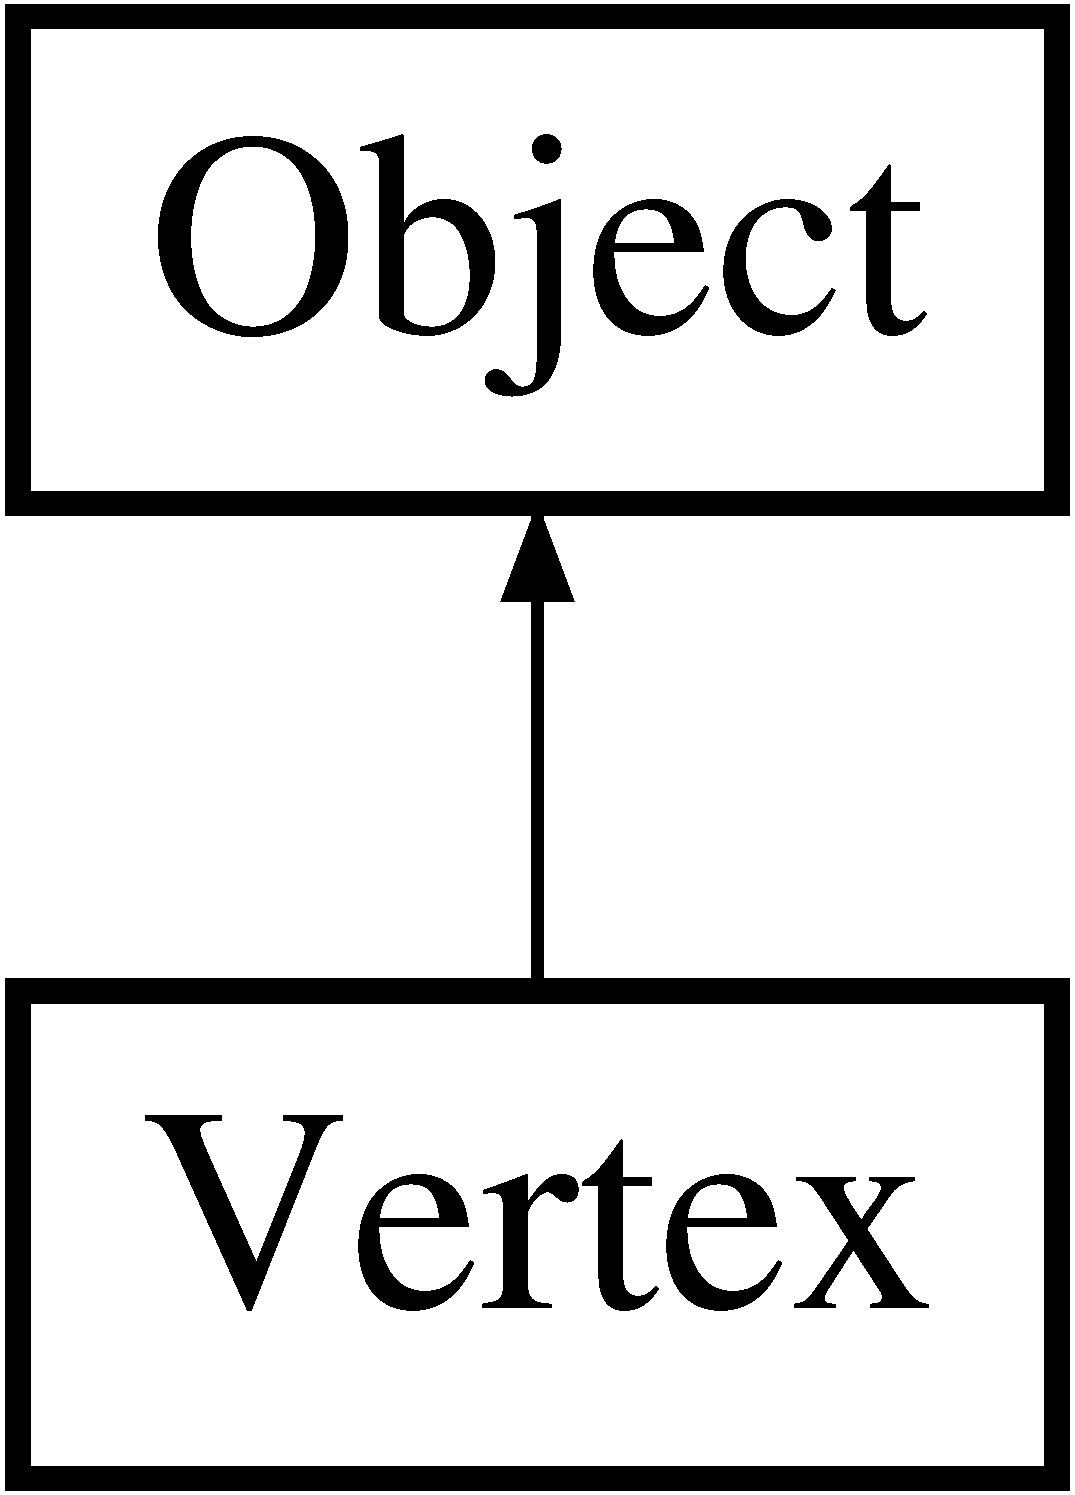
\includegraphics[height=2.000000cm]{class_vertex}
\end{center}
\end{figure}
\subsection*{Public Member Functions}
\begin{DoxyCompactItemize}
\item 
\hyperlink{class_vertex_a97488994a2482d70da74e1b91d40e169}{Vertex} ()
\begin{DoxyCompactList}\small\item\em Constructors. \end{DoxyCompactList}\item 
\hyperlink{class_vertex_a86a01a9679eed567448b8165ba335ddf}{Vertex} (const \hyperlink{class_vertex}{Vertex} \&vertex)
\item 
\hyperlink{class_vertex_ab3aaaa3fea9602eaf3d80c42702a6d5f}{Vertex} (X\+M\+F\+L\+O\+A\+T3 position)
\item 
\hyperlink{class_vertex_a2c558c054a0a2c970588c063073803a0}{Vertex} (float x, float y, float z)
\item 
\hyperlink{class_vertex_a9be3dce54b0ff2b0338ba00ba4307cab}{Vertex} (X\+M\+F\+L\+O\+A\+T3 position, D\+W\+O\+RD color, float u, float v)
\item 
\hyperlink{class_vertex_a00ab3eccce14fd1aa56662437977f40a}{Vertex} (float x, float y, float z, D\+W\+O\+RD color, float u, float v)
\item 
float \hyperlink{class_vertex_a8c00f077ae72434ebba3687b03135105}{Calculate\+Vector\+Length} ()
\begin{DoxyCompactList}\small\item\em Functions. \end{DoxyCompactList}\item 
void \hyperlink{class_vertex_a8094b5faac3ce2dd40a4d112133ffc73}{Normalize} ()
\item 
X\+M\+F\+L\+O\+A\+T3 \hyperlink{class_vertex_a96920908f0adadf6d6fef447013a32fc}{Get\+Position} ()
\begin{DoxyCompactList}\small\item\em Getters. \end{DoxyCompactList}\item 
float \hyperlink{class_vertex_a92792a1608974b53e87f7cba979cf97c}{GetX} ()
\item 
float \hyperlink{class_vertex_a89139909c6a69257d7d3b2234a01c304}{GetY} ()
\item 
float \hyperlink{class_vertex_afea768f12fdbb44ee051414fea2d44d0}{GetZ} ()
\item 
D\+W\+O\+RD \hyperlink{class_vertex_a636bda7b90b61dd6e23cc84c3781e5a5}{Get\+Color} ()
\item 
float \hyperlink{class_vertex_ada06e4d8d0f06652cb3b6a06776e1069}{GetU} ()
\item 
float \hyperlink{class_vertex_a05e50625839f1ce7b35574cdf443d64e}{GetV} ()
\item 
void \hyperlink{class_vertex_aa4c230ebaa8a0c0a8ca6a1e29d5ae93e}{Set\+Position} (X\+M\+F\+L\+O\+A\+T3 position)
\begin{DoxyCompactList}\small\item\em Setters. \end{DoxyCompactList}\item 
void \hyperlink{class_vertex_a05956877b676ad982b5e706ce726e44a}{SetX} (float x)
\item 
void \hyperlink{class_vertex_ad8b8b10e8e2f617c61be74aa50464293}{SetY} (float y)
\item 
void \hyperlink{class_vertex_ab488ce5e53970ae1172ba49417d85b07}{SetZ} (float z)
\item 
void \hyperlink{class_vertex_a5febdb33567ab2a7f06fc85a2614d526}{Set\+Color} (D\+W\+O\+RD color)
\item 
void \hyperlink{class_vertex_aebfd289c47c2c19c5655e0ccf1dac72f}{SetU} (float u)
\item 
void \hyperlink{class_vertex_a429f3b9b25ba1f58e09bfcf12c1029b6}{SetV} (float v)
\end{DoxyCompactItemize}
\subsection*{Static Public Member Functions}
\begin{DoxyCompactItemize}
\item 
static float \hyperlink{class_vertex_a6d31c2682560aaf39b12be7085f8a15d}{Calculate\+Vector\+Length} (\hyperlink{class_vertex}{Vertex} vector)
\item 
static float \hyperlink{class_vertex_a9aa994d5edcc65c5114142a818559098}{Calculate\+Vector\+Length} (X\+M\+F\+L\+O\+A\+T3 vector)
\item 
static float \hyperlink{class_vertex_a1f78e29eef1efb38d9bf6234e6d51a82}{Calculate\+Vector\+Length} (float x, float y, float z)
\item 
static \hyperlink{class_vertex}{Vertex} \hyperlink{class_vertex_a8ddc8aebbcc4226698bd2c85730f7748}{Normalize} (\hyperlink{class_vertex}{Vertex} vector\+To\+Normalize)
\item 
static X\+M\+F\+L\+O\+A\+T3 \hyperlink{class_vertex_a8080cc17ccbad289de853b6c8d53d416}{Normalize} (X\+M\+F\+L\+O\+A\+T3 vector\+To\+Normalize)
\end{DoxyCompactItemize}
\subsection*{Protected Attributes}
\begin{DoxyCompactItemize}
\item 
X\+M\+F\+L\+O\+A\+T3 \hyperlink{class_vertex_a476a5301ed5a6dfa7d7c9c52de29406d}{my\+Position}
\item 
D\+W\+O\+RD \hyperlink{class_vertex_a1d2fa85b4b70f8a850ad72cfb77086b5}{my\+Color}
\item 
float \hyperlink{class_vertex_af2e791591e89e6f39ad37329708f7470}{myU}
\item 
float \hyperlink{class_vertex_a4b26884b35841183664354eba0287aac}{myV}
\end{DoxyCompactItemize}


\subsection{Constructor \& Destructor Documentation}
\index{Vertex@{Vertex}!Vertex@{Vertex}}
\index{Vertex@{Vertex}!Vertex@{Vertex}}
\subsubsection[{\texorpdfstring{Vertex()}{Vertex()}}]{\setlength{\rightskip}{0pt plus 5cm}Vertex\+::\+Vertex (
\begin{DoxyParamCaption}
{}
\end{DoxyParamCaption}
)}\hypertarget{class_vertex_a97488994a2482d70da74e1b91d40e169}{}\label{class_vertex_a97488994a2482d70da74e1b91d40e169}


Constructors. 

Default Constructor.

\begin{DoxyAuthor}{Author}
Katianie 
\end{DoxyAuthor}
\begin{DoxyDate}{Date}
7/4/2016 
\end{DoxyDate}
\index{Vertex@{Vertex}!Vertex@{Vertex}}
\index{Vertex@{Vertex}!Vertex@{Vertex}}
\subsubsection[{\texorpdfstring{Vertex(const Vertex \&vertex)}{Vertex(const Vertex &vertex)}}]{\setlength{\rightskip}{0pt plus 5cm}Vertex\+::\+Vertex (
\begin{DoxyParamCaption}
\item[{const {\bf Vertex} \&}]{vertex}
\end{DoxyParamCaption}
)}\hypertarget{class_vertex_a86a01a9679eed567448b8165ba335ddf}{}\label{class_vertex_a86a01a9679eed567448b8165ba335ddf}
Copy constructor.

\begin{DoxyAuthor}{Author}
Katianie 
\end{DoxyAuthor}
\begin{DoxyDate}{Date}
7/4/2016
\end{DoxyDate}

\begin{DoxyParams}{Parameters}
{\em vertex} & The vertex. \\
\hline
\end{DoxyParams}
\index{Vertex@{Vertex}!Vertex@{Vertex}}
\index{Vertex@{Vertex}!Vertex@{Vertex}}
\subsubsection[{\texorpdfstring{Vertex(\+X\+M\+F\+L\+O\+A\+T3 position)}{Vertex(XMFLOAT3 position)}}]{\setlength{\rightskip}{0pt plus 5cm}Vertex\+::\+Vertex (
\begin{DoxyParamCaption}
\item[{X\+M\+F\+L\+O\+A\+T3}]{position}
\end{DoxyParamCaption}
)}\hypertarget{class_vertex_ab3aaaa3fea9602eaf3d80c42702a6d5f}{}\label{class_vertex_ab3aaaa3fea9602eaf3d80c42702a6d5f}
Constructor.

\begin{DoxyAuthor}{Author}
Katianie 
\end{DoxyAuthor}
\begin{DoxyDate}{Date}
7/4/2016
\end{DoxyDate}

\begin{DoxyParams}{Parameters}
{\em position} & The position. \\
\hline
\end{DoxyParams}
\index{Vertex@{Vertex}!Vertex@{Vertex}}
\index{Vertex@{Vertex}!Vertex@{Vertex}}
\subsubsection[{\texorpdfstring{Vertex(float x, float y, float z)}{Vertex(float x, float y, float z)}}]{\setlength{\rightskip}{0pt plus 5cm}Vertex\+::\+Vertex (
\begin{DoxyParamCaption}
\item[{float}]{x, }
\item[{float}]{y, }
\item[{float}]{z}
\end{DoxyParamCaption}
)}\hypertarget{class_vertex_a2c558c054a0a2c970588c063073803a0}{}\label{class_vertex_a2c558c054a0a2c970588c063073803a0}
Constructor.

\begin{DoxyAuthor}{Author}
Katianie 
\end{DoxyAuthor}
\begin{DoxyDate}{Date}
7/4/2016
\end{DoxyDate}

\begin{DoxyParams}{Parameters}
{\em x} & The x position coordinate. \\
\hline
{\em y} & The y position coordinate. \\
\hline
{\em z} & The z position coordinate. \\
\hline
\end{DoxyParams}
\index{Vertex@{Vertex}!Vertex@{Vertex}}
\index{Vertex@{Vertex}!Vertex@{Vertex}}
\subsubsection[{\texorpdfstring{Vertex(\+X\+M\+F\+L\+O\+A\+T3 position, D\+W\+O\+R\+D color, float u, float v)}{Vertex(XMFLOAT3 position, DWORD color, float u, float v)}}]{\setlength{\rightskip}{0pt plus 5cm}Vertex\+::\+Vertex (
\begin{DoxyParamCaption}
\item[{X\+M\+F\+L\+O\+A\+T3}]{position, }
\item[{D\+W\+O\+RD}]{color, }
\item[{float}]{u, }
\item[{float}]{v}
\end{DoxyParamCaption}
)}\hypertarget{class_vertex_a9be3dce54b0ff2b0338ba00ba4307cab}{}\label{class_vertex_a9be3dce54b0ff2b0338ba00ba4307cab}
Constructor.

\begin{DoxyAuthor}{Author}
Katianie 
\end{DoxyAuthor}
\begin{DoxyDate}{Date}
7/4/2016
\end{DoxyDate}

\begin{DoxyParams}{Parameters}
{\em position} & The position. \\
\hline
{\em color} & The color. \\
\hline
{\em u} & The u texture coordinate. \\
\hline
{\em v} & The v texture coordinate. \\
\hline
\end{DoxyParams}
\index{Vertex@{Vertex}!Vertex@{Vertex}}
\index{Vertex@{Vertex}!Vertex@{Vertex}}
\subsubsection[{\texorpdfstring{Vertex(float x, float y, float z, D\+W\+O\+R\+D color, float u, float v)}{Vertex(float x, float y, float z, DWORD color, float u, float v)}}]{\setlength{\rightskip}{0pt plus 5cm}Vertex\+::\+Vertex (
\begin{DoxyParamCaption}
\item[{float}]{x, }
\item[{float}]{y, }
\item[{float}]{z, }
\item[{D\+W\+O\+RD}]{color, }
\item[{float}]{u, }
\item[{float}]{v}
\end{DoxyParamCaption}
)}\hypertarget{class_vertex_a00ab3eccce14fd1aa56662437977f40a}{}\label{class_vertex_a00ab3eccce14fd1aa56662437977f40a}
Constructor.

\begin{DoxyAuthor}{Author}
Katianie 
\end{DoxyAuthor}
\begin{DoxyDate}{Date}
7/4/2016
\end{DoxyDate}

\begin{DoxyParams}{Parameters}
{\em x} & The x coordinate. \\
\hline
{\em y} & The y coordinate. \\
\hline
{\em z} & The z coordinate. \\
\hline
{\em color} & The color. \\
\hline
{\em u} & The u texture coordinate. \\
\hline
{\em v} & The v texture coordinate. \\
\hline
\end{DoxyParams}


\subsection{Member Function Documentation}
\index{Vertex@{Vertex}!Calculate\+Vector\+Length@{Calculate\+Vector\+Length}}
\index{Calculate\+Vector\+Length@{Calculate\+Vector\+Length}!Vertex@{Vertex}}
\subsubsection[{\texorpdfstring{Calculate\+Vector\+Length()}{CalculateVectorLength()}}]{\setlength{\rightskip}{0pt plus 5cm}float Vertex\+::\+Calculate\+Vector\+Length (
\begin{DoxyParamCaption}
{}
\end{DoxyParamCaption}
)}\hypertarget{class_vertex_a8c00f077ae72434ebba3687b03135105}{}\label{class_vertex_a8c00f077ae72434ebba3687b03135105}


Functions. 

Calculate the length of the vector.

\begin{DoxyAuthor}{Author}
Katianie 
\end{DoxyAuthor}
\begin{DoxyDate}{Date}
7/4/2016
\end{DoxyDate}
\begin{DoxyReturn}{Returns}
The calculated vector length. 
\end{DoxyReturn}
\index{Vertex@{Vertex}!Calculate\+Vector\+Length@{Calculate\+Vector\+Length}}
\index{Calculate\+Vector\+Length@{Calculate\+Vector\+Length}!Vertex@{Vertex}}
\subsubsection[{\texorpdfstring{Calculate\+Vector\+Length(\+Vertex vector)}{CalculateVectorLength(Vertex vector)}}]{\setlength{\rightskip}{0pt plus 5cm}float Vertex\+::\+Calculate\+Vector\+Length (
\begin{DoxyParamCaption}
\item[{{\bf Vertex}}]{vector}
\end{DoxyParamCaption}
)\hspace{0.3cm}{\ttfamily [static]}}\hypertarget{class_vertex_a6d31c2682560aaf39b12be7085f8a15d}{}\label{class_vertex_a6d31c2682560aaf39b12be7085f8a15d}
Calculates the length of the vector.

\begin{DoxyAuthor}{Author}
Katianie 
\end{DoxyAuthor}
\begin{DoxyDate}{Date}
7/4/2016
\end{DoxyDate}

\begin{DoxyParams}{Parameters}
{\em vector} & The vector.\\
\hline
\end{DoxyParams}
\begin{DoxyReturn}{Returns}
The calculated vector length. 
\end{DoxyReturn}
\index{Vertex@{Vertex}!Calculate\+Vector\+Length@{Calculate\+Vector\+Length}}
\index{Calculate\+Vector\+Length@{Calculate\+Vector\+Length}!Vertex@{Vertex}}
\subsubsection[{\texorpdfstring{Calculate\+Vector\+Length(\+X\+M\+F\+L\+O\+A\+T3 vector)}{CalculateVectorLength(XMFLOAT3 vector)}}]{\setlength{\rightskip}{0pt plus 5cm}float Vertex\+::\+Calculate\+Vector\+Length (
\begin{DoxyParamCaption}
\item[{X\+M\+F\+L\+O\+A\+T3}]{vector}
\end{DoxyParamCaption}
)\hspace{0.3cm}{\ttfamily [static]}}\hypertarget{class_vertex_a9aa994d5edcc65c5114142a818559098}{}\label{class_vertex_a9aa994d5edcc65c5114142a818559098}
Calculates the length of the vector.

\begin{DoxyAuthor}{Author}
Katianie 
\end{DoxyAuthor}
\begin{DoxyDate}{Date}
7/4/2016
\end{DoxyDate}

\begin{DoxyParams}{Parameters}
{\em vector} & The vector.\\
\hline
\end{DoxyParams}
\begin{DoxyReturn}{Returns}
The calculated vector length. 
\end{DoxyReturn}
\index{Vertex@{Vertex}!Calculate\+Vector\+Length@{Calculate\+Vector\+Length}}
\index{Calculate\+Vector\+Length@{Calculate\+Vector\+Length}!Vertex@{Vertex}}
\subsubsection[{\texorpdfstring{Calculate\+Vector\+Length(float x, float y, float z)}{CalculateVectorLength(float x, float y, float z)}}]{\setlength{\rightskip}{0pt plus 5cm}float Vertex\+::\+Calculate\+Vector\+Length (
\begin{DoxyParamCaption}
\item[{float}]{x, }
\item[{float}]{y, }
\item[{float}]{z}
\end{DoxyParamCaption}
)\hspace{0.3cm}{\ttfamily [static]}}\hypertarget{class_vertex_a1f78e29eef1efb38d9bf6234e6d51a82}{}\label{class_vertex_a1f78e29eef1efb38d9bf6234e6d51a82}
Calculates the length of the vector.

\begin{DoxyAuthor}{Author}
Katianie 
\end{DoxyAuthor}
\begin{DoxyDate}{Date}
7/4/2016
\end{DoxyDate}

\begin{DoxyParams}{Parameters}
{\em x} & The x coordinate. \\
\hline
{\em y} & The y coordinate. \\
\hline
{\em z} & The z coordinate.\\
\hline
\end{DoxyParams}
\begin{DoxyReturn}{Returns}
The calculated vector length. 
\end{DoxyReturn}
\index{Vertex@{Vertex}!Get\+Color@{Get\+Color}}
\index{Get\+Color@{Get\+Color}!Vertex@{Vertex}}
\subsubsection[{\texorpdfstring{Get\+Color()}{GetColor()}}]{\setlength{\rightskip}{0pt plus 5cm}D\+W\+O\+RD Vertex\+::\+Get\+Color (
\begin{DoxyParamCaption}
{}
\end{DoxyParamCaption}
)}\hypertarget{class_vertex_a636bda7b90b61dd6e23cc84c3781e5a5}{}\label{class_vertex_a636bda7b90b61dd6e23cc84c3781e5a5}
Gets the color.

\begin{DoxyAuthor}{Author}
Katianie 
\end{DoxyAuthor}
\begin{DoxyDate}{Date}
7/4/2016
\end{DoxyDate}
\begin{DoxyReturn}{Returns}
The color. 
\end{DoxyReturn}
\index{Vertex@{Vertex}!Get\+Position@{Get\+Position}}
\index{Get\+Position@{Get\+Position}!Vertex@{Vertex}}
\subsubsection[{\texorpdfstring{Get\+Position()}{GetPosition()}}]{\setlength{\rightskip}{0pt plus 5cm}X\+M\+F\+L\+O\+A\+T3 Vertex\+::\+Get\+Position (
\begin{DoxyParamCaption}
{}
\end{DoxyParamCaption}
)}\hypertarget{class_vertex_a96920908f0adadf6d6fef447013a32fc}{}\label{class_vertex_a96920908f0adadf6d6fef447013a32fc}


Getters. 

Gets the position.

\begin{DoxyAuthor}{Author}
Katianie 
\end{DoxyAuthor}
\begin{DoxyDate}{Date}
7/4/2016
\end{DoxyDate}
\begin{DoxyReturn}{Returns}
The position. 
\end{DoxyReturn}
\index{Vertex@{Vertex}!GetU@{GetU}}
\index{GetU@{GetU}!Vertex@{Vertex}}
\subsubsection[{\texorpdfstring{Get\+U()}{GetU()}}]{\setlength{\rightskip}{0pt plus 5cm}float Vertex\+::\+GetU (
\begin{DoxyParamCaption}
{}
\end{DoxyParamCaption}
)}\hypertarget{class_vertex_ada06e4d8d0f06652cb3b6a06776e1069}{}\label{class_vertex_ada06e4d8d0f06652cb3b6a06776e1069}
Gets the u \hyperlink{class_texture}{Texture} coordinate.

\begin{DoxyAuthor}{Author}
Katianie 
\end{DoxyAuthor}
\begin{DoxyDate}{Date}
7/4/2016
\end{DoxyDate}
\begin{DoxyReturn}{Returns}
The u \hyperlink{class_texture}{Texture} coordinate. 
\end{DoxyReturn}
\index{Vertex@{Vertex}!GetV@{GetV}}
\index{GetV@{GetV}!Vertex@{Vertex}}
\subsubsection[{\texorpdfstring{Get\+V()}{GetV()}}]{\setlength{\rightskip}{0pt plus 5cm}float Vertex\+::\+GetV (
\begin{DoxyParamCaption}
{}
\end{DoxyParamCaption}
)}\hypertarget{class_vertex_a05e50625839f1ce7b35574cdf443d64e}{}\label{class_vertex_a05e50625839f1ce7b35574cdf443d64e}
Gets the v \hyperlink{class_texture}{Texture} coordinate.

\begin{DoxyAuthor}{Author}
Katianie 
\end{DoxyAuthor}
\begin{DoxyDate}{Date}
7/4/2016
\end{DoxyDate}
\begin{DoxyReturn}{Returns}
The v \hyperlink{class_texture}{Texture} coordinate. 
\end{DoxyReturn}
\index{Vertex@{Vertex}!GetX@{GetX}}
\index{GetX@{GetX}!Vertex@{Vertex}}
\subsubsection[{\texorpdfstring{Get\+X()}{GetX()}}]{\setlength{\rightskip}{0pt plus 5cm}float Vertex\+::\+GetX (
\begin{DoxyParamCaption}
{}
\end{DoxyParamCaption}
)}\hypertarget{class_vertex_a92792a1608974b53e87f7cba979cf97c}{}\label{class_vertex_a92792a1608974b53e87f7cba979cf97c}
Get x coordinate of the position.

\begin{DoxyAuthor}{Author}
Katianie 
\end{DoxyAuthor}
\begin{DoxyDate}{Date}
7/4/2016
\end{DoxyDate}
\begin{DoxyReturn}{Returns}
The x coordinate of the position. 
\end{DoxyReturn}
\index{Vertex@{Vertex}!GetY@{GetY}}
\index{GetY@{GetY}!Vertex@{Vertex}}
\subsubsection[{\texorpdfstring{Get\+Y()}{GetY()}}]{\setlength{\rightskip}{0pt plus 5cm}float Vertex\+::\+GetY (
\begin{DoxyParamCaption}
{}
\end{DoxyParamCaption}
)}\hypertarget{class_vertex_a89139909c6a69257d7d3b2234a01c304}{}\label{class_vertex_a89139909c6a69257d7d3b2234a01c304}
Get y coordinate of the position.

\begin{DoxyAuthor}{Author}
Katianie 
\end{DoxyAuthor}
\begin{DoxyDate}{Date}
7/4/2016
\end{DoxyDate}
\begin{DoxyReturn}{Returns}
The y coordinate of the position. 
\end{DoxyReturn}
\index{Vertex@{Vertex}!GetZ@{GetZ}}
\index{GetZ@{GetZ}!Vertex@{Vertex}}
\subsubsection[{\texorpdfstring{Get\+Z()}{GetZ()}}]{\setlength{\rightskip}{0pt plus 5cm}float Vertex\+::\+GetZ (
\begin{DoxyParamCaption}
{}
\end{DoxyParamCaption}
)}\hypertarget{class_vertex_afea768f12fdbb44ee051414fea2d44d0}{}\label{class_vertex_afea768f12fdbb44ee051414fea2d44d0}
Get z coordinate of the position.

\begin{DoxyAuthor}{Author}
Katianie 
\end{DoxyAuthor}
\begin{DoxyDate}{Date}
7/4/2016
\end{DoxyDate}
\begin{DoxyReturn}{Returns}
The z coordinate of the position. 
\end{DoxyReturn}
\index{Vertex@{Vertex}!Normalize@{Normalize}}
\index{Normalize@{Normalize}!Vertex@{Vertex}}
\subsubsection[{\texorpdfstring{Normalize()}{Normalize()}}]{\setlength{\rightskip}{0pt plus 5cm}void Vertex\+::\+Normalize (
\begin{DoxyParamCaption}
{}
\end{DoxyParamCaption}
)}\hypertarget{class_vertex_a8094b5faac3ce2dd40a4d112133ffc73}{}\label{class_vertex_a8094b5faac3ce2dd40a4d112133ffc73}
Normalizes my\+Position.

\begin{DoxyAuthor}{Author}
Katianie 
\end{DoxyAuthor}
\begin{DoxyDate}{Date}
7/4/2016 
\end{DoxyDate}
\index{Vertex@{Vertex}!Normalize@{Normalize}}
\index{Normalize@{Normalize}!Vertex@{Vertex}}
\subsubsection[{\texorpdfstring{Normalize(\+Vertex vector\+To\+Normalize)}{Normalize(Vertex vectorToNormalize)}}]{\setlength{\rightskip}{0pt plus 5cm}{\bf Vertex} Vertex\+::\+Normalize (
\begin{DoxyParamCaption}
\item[{{\bf Vertex}}]{vector\+To\+Normalize}
\end{DoxyParamCaption}
)\hspace{0.3cm}{\ttfamily [static]}}\hypertarget{class_vertex_a8ddc8aebbcc4226698bd2c85730f7748}{}\label{class_vertex_a8ddc8aebbcc4226698bd2c85730f7748}
Normalizes the given vector.

\begin{DoxyAuthor}{Author}
Katianie 
\end{DoxyAuthor}
\begin{DoxyDate}{Date}
7/4/2016
\end{DoxyDate}

\begin{DoxyParams}{Parameters}
{\em vector\+To\+Normalize} & The vector to normalize.\\
\hline
\end{DoxyParams}
\begin{DoxyReturn}{Returns}
A vertex containing a normalized position. 
\end{DoxyReturn}
\index{Vertex@{Vertex}!Normalize@{Normalize}}
\index{Normalize@{Normalize}!Vertex@{Vertex}}
\subsubsection[{\texorpdfstring{Normalize(\+X\+M\+F\+L\+O\+A\+T3 vector\+To\+Normalize)}{Normalize(XMFLOAT3 vectorToNormalize)}}]{\setlength{\rightskip}{0pt plus 5cm}X\+M\+F\+L\+O\+A\+T3 Vertex\+::\+Normalize (
\begin{DoxyParamCaption}
\item[{X\+M\+F\+L\+O\+A\+T3}]{vector\+To\+Normalize}
\end{DoxyParamCaption}
)\hspace{0.3cm}{\ttfamily [static]}}\hypertarget{class_vertex_a8080cc17ccbad289de853b6c8d53d416}{}\label{class_vertex_a8080cc17ccbad289de853b6c8d53d416}
Normalizes the given vector.

\begin{DoxyAuthor}{Author}
Katianie 
\end{DoxyAuthor}
\begin{DoxyDate}{Date}
7/4/2016
\end{DoxyDate}

\begin{DoxyParams}{Parameters}
{\em vector\+To\+Normalize} & The vector to normalize.\\
\hline
\end{DoxyParams}
\begin{DoxyReturn}{Returns}
An X\+M\+F\+L\+O\+A\+T3. 
\end{DoxyReturn}
\index{Vertex@{Vertex}!Set\+Color@{Set\+Color}}
\index{Set\+Color@{Set\+Color}!Vertex@{Vertex}}
\subsubsection[{\texorpdfstring{Set\+Color(\+D\+W\+O\+R\+D color)}{SetColor(DWORD color)}}]{\setlength{\rightskip}{0pt plus 5cm}void Vertex\+::\+Set\+Color (
\begin{DoxyParamCaption}
\item[{D\+W\+O\+RD}]{color}
\end{DoxyParamCaption}
)}\hypertarget{class_vertex_a5febdb33567ab2a7f06fc85a2614d526}{}\label{class_vertex_a5febdb33567ab2a7f06fc85a2614d526}
Sets a color.

\begin{DoxyAuthor}{Author}
Katianie 
\end{DoxyAuthor}
\begin{DoxyDate}{Date}
7/4/2016
\end{DoxyDate}

\begin{DoxyParams}{Parameters}
{\em color} & The color. \\
\hline
\end{DoxyParams}
\index{Vertex@{Vertex}!Set\+Position@{Set\+Position}}
\index{Set\+Position@{Set\+Position}!Vertex@{Vertex}}
\subsubsection[{\texorpdfstring{Set\+Position(\+X\+M\+F\+L\+O\+A\+T3 position)}{SetPosition(XMFLOAT3 position)}}]{\setlength{\rightskip}{0pt plus 5cm}void Vertex\+::\+Set\+Position (
\begin{DoxyParamCaption}
\item[{X\+M\+F\+L\+O\+A\+T3}]{position}
\end{DoxyParamCaption}
)}\hypertarget{class_vertex_aa4c230ebaa8a0c0a8ca6a1e29d5ae93e}{}\label{class_vertex_aa4c230ebaa8a0c0a8ca6a1e29d5ae93e}


Setters. 

Sets the position.

\begin{DoxyAuthor}{Author}
Katianie 
\end{DoxyAuthor}
\begin{DoxyDate}{Date}
7/4/2016
\end{DoxyDate}

\begin{DoxyParams}{Parameters}
{\em position} & The position. \\
\hline
\end{DoxyParams}
\index{Vertex@{Vertex}!SetU@{SetU}}
\index{SetU@{SetU}!Vertex@{Vertex}}
\subsubsection[{\texorpdfstring{Set\+U(float u)}{SetU(float u)}}]{\setlength{\rightskip}{0pt plus 5cm}void Vertex\+::\+SetU (
\begin{DoxyParamCaption}
\item[{float}]{u}
\end{DoxyParamCaption}
)}\hypertarget{class_vertex_aebfd289c47c2c19c5655e0ccf1dac72f}{}\label{class_vertex_aebfd289c47c2c19c5655e0ccf1dac72f}
Sets a u \hyperlink{class_texture}{Texture} coordinate.

\begin{DoxyAuthor}{Author}
Katianie 
\end{DoxyAuthor}
\begin{DoxyDate}{Date}
7/4/2016
\end{DoxyDate}

\begin{DoxyParams}{Parameters}
{\em u} & The u \hyperlink{class_texture}{Texture} coordinate. \\
\hline
\end{DoxyParams}
\index{Vertex@{Vertex}!SetV@{SetV}}
\index{SetV@{SetV}!Vertex@{Vertex}}
\subsubsection[{\texorpdfstring{Set\+V(float v)}{SetV(float v)}}]{\setlength{\rightskip}{0pt plus 5cm}void Vertex\+::\+SetV (
\begin{DoxyParamCaption}
\item[{float}]{v}
\end{DoxyParamCaption}
)}\hypertarget{class_vertex_a429f3b9b25ba1f58e09bfcf12c1029b6}{}\label{class_vertex_a429f3b9b25ba1f58e09bfcf12c1029b6}
Sets a v \hyperlink{class_texture}{Texture} coordinate.

\begin{DoxyAuthor}{Author}
Katianie 
\end{DoxyAuthor}
\begin{DoxyDate}{Date}
7/4/2016
\end{DoxyDate}

\begin{DoxyParams}{Parameters}
{\em v} & The v \hyperlink{class_texture}{Texture} coordinate. \\
\hline
\end{DoxyParams}
\index{Vertex@{Vertex}!SetX@{SetX}}
\index{SetX@{SetX}!Vertex@{Vertex}}
\subsubsection[{\texorpdfstring{Set\+X(float x)}{SetX(float x)}}]{\setlength{\rightskip}{0pt plus 5cm}void Vertex\+::\+SetX (
\begin{DoxyParamCaption}
\item[{float}]{x}
\end{DoxyParamCaption}
)}\hypertarget{class_vertex_a05956877b676ad982b5e706ce726e44a}{}\label{class_vertex_a05956877b676ad982b5e706ce726e44a}
Sets the x coordinate of the position.

\begin{DoxyAuthor}{Author}
Katianie 
\end{DoxyAuthor}
\begin{DoxyDate}{Date}
7/4/2016
\end{DoxyDate}

\begin{DoxyParams}{Parameters}
{\em x} & The x coordinate of the position. \\
\hline
\end{DoxyParams}
\index{Vertex@{Vertex}!SetY@{SetY}}
\index{SetY@{SetY}!Vertex@{Vertex}}
\subsubsection[{\texorpdfstring{Set\+Y(float y)}{SetY(float y)}}]{\setlength{\rightskip}{0pt plus 5cm}void Vertex\+::\+SetY (
\begin{DoxyParamCaption}
\item[{float}]{y}
\end{DoxyParamCaption}
)}\hypertarget{class_vertex_ad8b8b10e8e2f617c61be74aa50464293}{}\label{class_vertex_ad8b8b10e8e2f617c61be74aa50464293}
Sets a y coordinate of the position.

\begin{DoxyAuthor}{Author}
Katianie 
\end{DoxyAuthor}
\begin{DoxyDate}{Date}
7/4/2016
\end{DoxyDate}

\begin{DoxyParams}{Parameters}
{\em y} & The y coordinate of the position. \\
\hline
\end{DoxyParams}
\index{Vertex@{Vertex}!SetZ@{SetZ}}
\index{SetZ@{SetZ}!Vertex@{Vertex}}
\subsubsection[{\texorpdfstring{Set\+Z(float z)}{SetZ(float z)}}]{\setlength{\rightskip}{0pt plus 5cm}void Vertex\+::\+SetZ (
\begin{DoxyParamCaption}
\item[{float}]{z}
\end{DoxyParamCaption}
)}\hypertarget{class_vertex_ab488ce5e53970ae1172ba49417d85b07}{}\label{class_vertex_ab488ce5e53970ae1172ba49417d85b07}
Sets a z coordinate of the position.

\begin{DoxyAuthor}{Author}
Katianie 
\end{DoxyAuthor}
\begin{DoxyDate}{Date}
7/4/2016
\end{DoxyDate}

\begin{DoxyParams}{Parameters}
{\em z} & The z coordinate of the position. \\
\hline
\end{DoxyParams}


\subsection{Member Data Documentation}
\index{Vertex@{Vertex}!my\+Color@{my\+Color}}
\index{my\+Color@{my\+Color}!Vertex@{Vertex}}
\subsubsection[{\texorpdfstring{my\+Color}{myColor}}]{\setlength{\rightskip}{0pt plus 5cm}D\+W\+O\+RD Vertex\+::my\+Color\hspace{0.3cm}{\ttfamily [protected]}}\hypertarget{class_vertex_a1d2fa85b4b70f8a850ad72cfb77086b5}{}\label{class_vertex_a1d2fa85b4b70f8a850ad72cfb77086b5}
\index{Vertex@{Vertex}!my\+Position@{my\+Position}}
\index{my\+Position@{my\+Position}!Vertex@{Vertex}}
\subsubsection[{\texorpdfstring{my\+Position}{myPosition}}]{\setlength{\rightskip}{0pt plus 5cm}X\+M\+F\+L\+O\+A\+T3 Vertex\+::my\+Position\hspace{0.3cm}{\ttfamily [protected]}}\hypertarget{class_vertex_a476a5301ed5a6dfa7d7c9c52de29406d}{}\label{class_vertex_a476a5301ed5a6dfa7d7c9c52de29406d}
\index{Vertex@{Vertex}!myU@{myU}}
\index{myU@{myU}!Vertex@{Vertex}}
\subsubsection[{\texorpdfstring{myU}{myU}}]{\setlength{\rightskip}{0pt plus 5cm}float Vertex\+::myU\hspace{0.3cm}{\ttfamily [protected]}}\hypertarget{class_vertex_af2e791591e89e6f39ad37329708f7470}{}\label{class_vertex_af2e791591e89e6f39ad37329708f7470}
\index{Vertex@{Vertex}!myV@{myV}}
\index{myV@{myV}!Vertex@{Vertex}}
\subsubsection[{\texorpdfstring{myV}{myV}}]{\setlength{\rightskip}{0pt plus 5cm}float Vertex\+::myV\hspace{0.3cm}{\ttfamily [protected]}}\hypertarget{class_vertex_a4b26884b35841183664354eba0287aac}{}\label{class_vertex_a4b26884b35841183664354eba0287aac}


The documentation for this class was generated from the following files\+:\begin{DoxyCompactItemize}
\item 
Samples/\+Oculus\+Room\+Tiny\+\_\+\+Advanced/\+Common/\+Headers/\hyperlink{_vertex_8h}{Vertex.\+h}\item 
Samples/\+Oculus\+Room\+Tiny\+\_\+\+Advanced/\+Common/\+Implementations/\hyperlink{_vertex_8cpp}{Vertex.\+cpp}\end{DoxyCompactItemize}

\hypertarget{class_v_r_layer}{}\section{V\+R\+Layer Class Reference}
\label{class_v_r_layer}\index{V\+R\+Layer@{V\+R\+Layer}}


{\ttfamily \#include $<$V\+R\+Layer.\+h$>$}

Inheritance diagram for V\+R\+Layer\+:\begin{figure}[H]
\begin{center}
\leavevmode
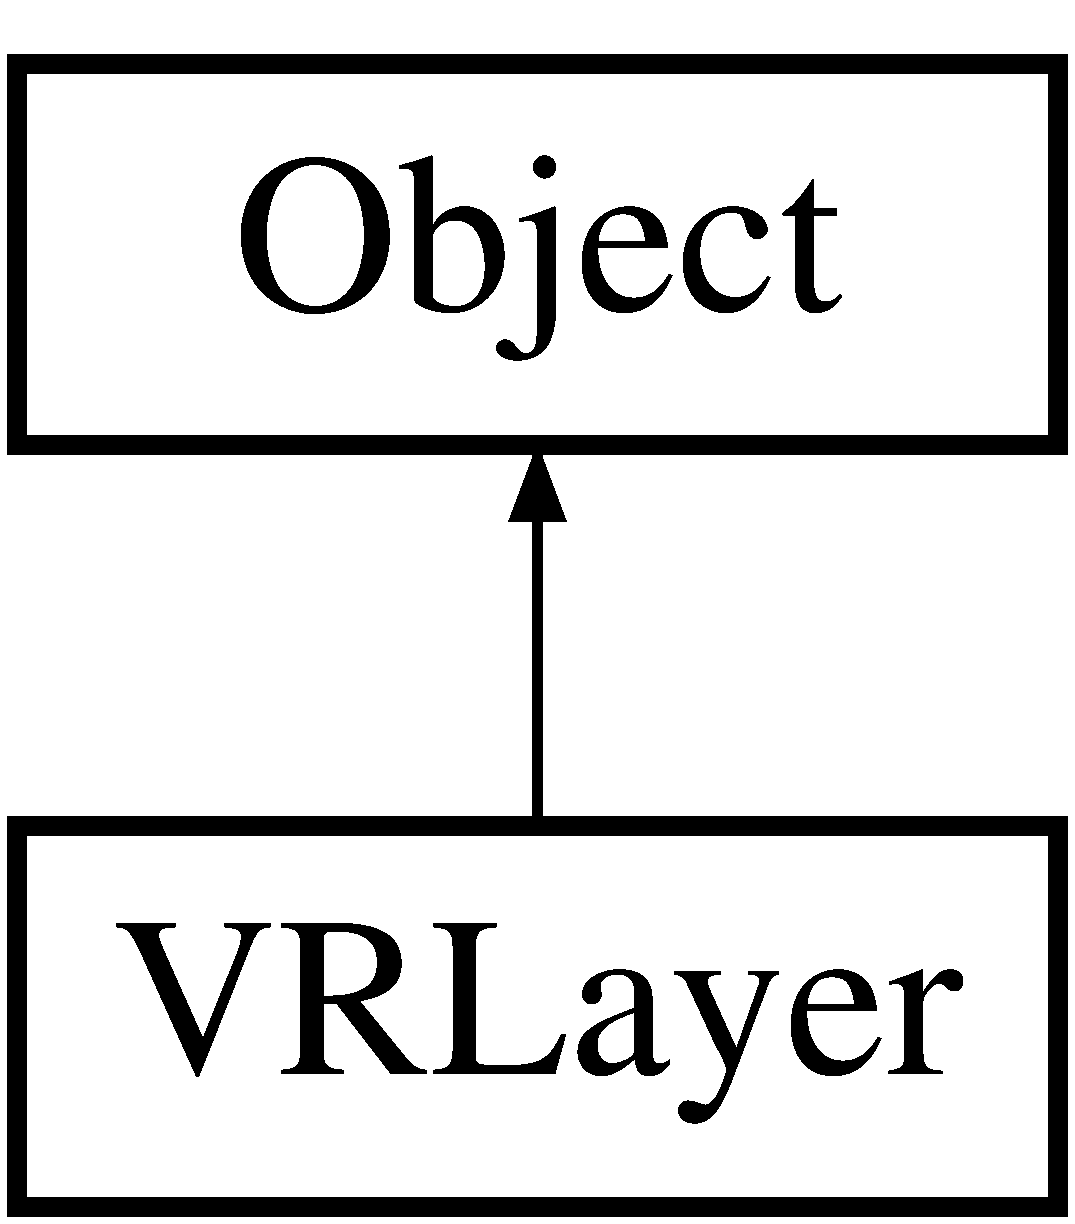
\includegraphics[height=2.000000cm]{class_v_r_layer}
\end{center}
\end{figure}
\subsection*{Public Member Functions}
\begin{DoxyCompactItemize}
\item 
\hyperlink{class_v_r_layer_a16cea0d400080518b73a30c2ac38d2d6}{V\+R\+Layer} (ovr\+Hmd hmd, const ovr\+Fov\+Port $\ast$fovs=N\+U\+LL, float pixels\+Per\+Display\+Pixel=1.\+0f)
\begin{DoxyCompactList}\small\item\em Constructor. \end{DoxyCompactList}\item 
virtual \hyperlink{class_v_r_layer_a673f6e38b025c92bb4397d223b1b30fa}{$\sim$\+V\+R\+Layer} ()
\begin{DoxyCompactList}\small\item\em Destructor. \end{DoxyCompactList}\item 
ovr\+Tracking\+State \hyperlink{class_v_r_layer_ab942320f67671f92e2e0c15c6a68ee78}{Calculate\+Eye\+Poses} ()
\begin{DoxyCompactList}\small\item\em Functions. \end{DoxyCompactList}\item 
void \hyperlink{class_v_r_layer_adc020df4324c1a9fd3eb4b87ea7b2b16}{Initialize\+Layer\+Header} ()
\item 
void \hyperlink{class_v_r_layer_a37225d61e04354b44647bf7e895da76b}{Make\+Eye\+Buffers} (float pixels\+Per\+Display\+Pixel=1.\+0f)
\item 
void \hyperlink{class_v_r_layer_a8941a91820ed1e6cac2a3fc3bbb9529d}{Modify\+F\+O\+VS} (const ovr\+Fov\+Port $\ast$fovs=N\+U\+LL)
\item 
X\+M\+M\+A\+T\+R\+IX \hyperlink{class_v_r_layer_a3e9bfdfff5a069783b084e0a12b1d292}{Render\+Scene\+To\+Eye\+Buffer} (\hyperlink{class_camera}{Camera} $\ast$player\+Camera, \hyperlink{class_scene}{Scene} $\ast$scene\+To\+Render, int eye\+Index, I\+D3\+D11\+Render\+Target\+View $\ast$render\+Target=N\+U\+LL, ovr\+Posef $\ast$eye\+Render\+Pose=N\+U\+LL, int times\+To\+Render\+Room=1, float alpha=1.\+0f, float red=1.\+0f, float green=1.\+0f, float blue=1.\+0f, float near\+Z=0.\+2f, float far\+Z=1000.\+0f, bool do\+We\+Setup\+Render=true, Depth\+Buffer $\ast$depth\+Buffer=\+N\+U\+L\+L, float back\+Red=0.\+0f, float back\+Green=0.\+0f, float back\+Blue=0.\+0f)
\item 
\hyperlink{class_depth_buffer}{Depth\+Buffer} $\ast$$\ast$ \hyperlink{class_v_r_layer_a1dd1511b144b8d3ec95248c9c3bb5ce0}{Get\+Eye\+Depth\+Buffers} ()
\begin{DoxyCompactList}\small\item\em Getters. \end{DoxyCompactList}\item 
ovr\+Eye\+Render\+Desc $\ast$ \hyperlink{class_v_r_layer_af0f7b3a0aec2d5175ae334ffa60bcdfd}{Get\+Eye\+Render\+Descriptions} ()
\item 
ovr\+Posef $\ast$ \hyperlink{class_v_r_layer_a9e90f858498e244c77482906bfefbd62}{Get\+Eye\+Render\+Poses} ()
\item 
\hyperlink{class_oculus_texture}{Oculus\+Texture} $\ast$$\ast$ \hyperlink{class_v_r_layer_a4c4ec79e724a3f179f15a64d5e1287f0}{Get\+Eye\+Render\+Textures} ()
\item 
ovr\+Recti $\ast$ \hyperlink{class_v_r_layer_abdb1657fca98fe38f25ac5806af70a0d}{Get\+Eye\+Render\+Viewports} ()
\item 
ovr\+Hmd \hyperlink{class_v_r_layer_ad7d68fc8325f5d8588dda33edd8b63f0}{Get\+H\+MD} ()
\item 
ovr\+Layer\+Eye\+Fov \& \hyperlink{class_v_r_layer_a338e5d2fd9c1f38c0757eeb735d5fe41}{Get\+Ovr\+Layer} ()
\end{DoxyCompactItemize}
\subsection*{Protected Attributes}
\begin{DoxyCompactItemize}
\item 
\hyperlink{class_depth_buffer}{Depth\+Buffer} $\ast$ \hyperlink{class_v_r_layer_a158518a0d3b7437032bb8b9dd513830f}{my\+Eye\+Depth\+Buffers} \mbox{[}2\mbox{]}
\item 
ovr\+Eye\+Render\+Desc \hyperlink{class_v_r_layer_a61e147e1041337a9849d3618aa782a82}{my\+Eye\+Render\+Descriptions} \mbox{[}2\mbox{]}
\item 
ovr\+Posef \hyperlink{class_v_r_layer_a0429a4b04ab3c5e51f5bd638519acfa3}{my\+Eye\+Render\+Poses} \mbox{[}2\mbox{]}
\item 
\hyperlink{class_oculus_texture}{Oculus\+Texture} $\ast$ \hyperlink{class_v_r_layer_a47a680aacb39848eff2148445cbba172}{my\+Eye\+Render\+Textures} \mbox{[}2\mbox{]}
\item 
ovr\+Recti \hyperlink{class_v_r_layer_ab79ac408b474f49eb0ec4fb5603752ff}{my\+Eye\+Render\+Viewports} \mbox{[}2\mbox{]}
\item 
ovr\+Hmd \hyperlink{class_v_r_layer_ab7dbb8c74485a7546bd77f6817e76da2}{my\+H\+MD}
\item 
ovr\+Layer\+Eye\+Fov \hyperlink{class_v_r_layer_a427baf6b2cb1ef51254fd83d0c9179f8}{my\+Ovr\+Layer}
\end{DoxyCompactItemize}
\subsection*{Additional Inherited Members}


\subsection{Constructor \& Destructor Documentation}
\index{V\+R\+Layer@{V\+R\+Layer}!V\+R\+Layer@{V\+R\+Layer}}
\index{V\+R\+Layer@{V\+R\+Layer}!V\+R\+Layer@{V\+R\+Layer}}
\subsubsection[{\texorpdfstring{V\+R\+Layer(ovr\+Hmd hmd, const ovr\+Fov\+Port $\ast$fovs=\+N\+U\+L\+L, float pixels\+Per\+Display\+Pixel=1.\+0f)}{VRLayer(ovrHmd hmd, const ovrFovPort *fovs=NULL, float pixelsPerDisplayPixel=1.0f)}}]{\setlength{\rightskip}{0pt plus 5cm}V\+R\+Layer\+::\+V\+R\+Layer (
\begin{DoxyParamCaption}
\item[{ovr\+Hmd}]{hmd, }
\item[{const ovr\+Fov\+Port $\ast$}]{fovs = {\ttfamily NULL}, }
\item[{float}]{pixels\+Per\+Display\+Pixel = {\ttfamily 1.0f}}
\end{DoxyParamCaption}
)}\hypertarget{class_v_r_layer_a16cea0d400080518b73a30c2ac38d2d6}{}\label{class_v_r_layer_a16cea0d400080518b73a30c2ac38d2d6}


Constructor. 

Constructor. Initialize O\+VR Field of View and other things such as buffer initialization. Each eye has a VR Layer, so for us there are two V\+R\+Layers.

\begin{DoxyAuthor}{Author}
Katianie 
\end{DoxyAuthor}
\begin{DoxyDate}{Date}
7/4/2016
\end{DoxyDate}

\begin{DoxyParams}{Parameters}
{\em hmd} & The H\+MD object. \\
\hline
{\em fovs} & Custom F\+OV for the H\+MD. \\
\hline
{\em pixels\+Per\+Display\+Pixel} & Default is 1.\+0, lower is better performance, higher is better quality. \\
\hline
\end{DoxyParams}
\index{V\+R\+Layer@{V\+R\+Layer}!````~V\+R\+Layer@{$\sim$\+V\+R\+Layer}}
\index{````~V\+R\+Layer@{$\sim$\+V\+R\+Layer}!V\+R\+Layer@{V\+R\+Layer}}
\subsubsection[{\texorpdfstring{$\sim$\+V\+R\+Layer()}{~VRLayer()}}]{\setlength{\rightskip}{0pt plus 5cm}V\+R\+Layer\+::$\sim$\+V\+R\+Layer (
\begin{DoxyParamCaption}
{}
\end{DoxyParamCaption}
)\hspace{0.3cm}{\ttfamily [virtual]}}\hypertarget{class_v_r_layer_a673f6e38b025c92bb4397d223b1b30fa}{}\label{class_v_r_layer_a673f6e38b025c92bb4397d223b1b30fa}


Destructor. 

Destructor.

\begin{DoxyAuthor}{Author}
Katianie 
\end{DoxyAuthor}
\begin{DoxyDate}{Date}
7/4/2016 
\end{DoxyDate}


\subsection{Member Function Documentation}
\index{V\+R\+Layer@{V\+R\+Layer}!Calculate\+Eye\+Poses@{Calculate\+Eye\+Poses}}
\index{Calculate\+Eye\+Poses@{Calculate\+Eye\+Poses}!V\+R\+Layer@{V\+R\+Layer}}
\subsubsection[{\texorpdfstring{Calculate\+Eye\+Poses()}{CalculateEyePoses()}}]{\setlength{\rightskip}{0pt plus 5cm}ovr\+Tracking\+State V\+R\+Layer\+::\+Calculate\+Eye\+Poses (
\begin{DoxyParamCaption}
{}
\end{DoxyParamCaption}
)}\hypertarget{class_v_r_layer_ab942320f67671f92e2e0c15c6a68ee78}{}\label{class_v_r_layer_ab942320f67671f92e2e0c15c6a68ee78}


Functions. 

Calculates the current eye poses. This needs to be updated constantly so we know the current position and orientation of the H\+MD.

\begin{DoxyAuthor}{Author}
Katianie 
\end{DoxyAuthor}
\begin{DoxyDate}{Date}
7/4/2016
\end{DoxyDate}
\begin{DoxyReturn}{Returns}
A struct containing the calculated eye poses. 
\end{DoxyReturn}
\index{V\+R\+Layer@{V\+R\+Layer}!Get\+Eye\+Depth\+Buffers@{Get\+Eye\+Depth\+Buffers}}
\index{Get\+Eye\+Depth\+Buffers@{Get\+Eye\+Depth\+Buffers}!V\+R\+Layer@{V\+R\+Layer}}
\subsubsection[{\texorpdfstring{Get\+Eye\+Depth\+Buffers()}{GetEyeDepthBuffers()}}]{\setlength{\rightskip}{0pt plus 5cm}{\bf Depth\+Buffer} $\ast$$\ast$ V\+R\+Layer\+::\+Get\+Eye\+Depth\+Buffers (
\begin{DoxyParamCaption}
{}
\end{DoxyParamCaption}
)}\hypertarget{class_v_r_layer_a1dd1511b144b8d3ec95248c9c3bb5ce0}{}\label{class_v_r_layer_a1dd1511b144b8d3ec95248c9c3bb5ce0}


Getters. 

Gets the array of Eye Depth buffers which are responsible for storing Z-\/\+Buffer data for each eye.

\begin{DoxyAuthor}{Author}
Katianie 
\end{DoxyAuthor}
\begin{DoxyDate}{Date}
7/5/2016
\end{DoxyDate}
\begin{DoxyReturn}{Returns}
The array of Eye Depth buffers. 
\end{DoxyReturn}
\index{V\+R\+Layer@{V\+R\+Layer}!Get\+Eye\+Render\+Descriptions@{Get\+Eye\+Render\+Descriptions}}
\index{Get\+Eye\+Render\+Descriptions@{Get\+Eye\+Render\+Descriptions}!V\+R\+Layer@{V\+R\+Layer}}
\subsubsection[{\texorpdfstring{Get\+Eye\+Render\+Descriptions()}{GetEyeRenderDescriptions()}}]{\setlength{\rightskip}{0pt plus 5cm}ovr\+Eye\+Render\+Desc $\ast$ V\+R\+Layer\+::\+Get\+Eye\+Render\+Descriptions (
\begin{DoxyParamCaption}
{}
\end{DoxyParamCaption}
)}\hypertarget{class_v_r_layer_af0f7b3a0aec2d5175ae334ffa60bcdfd}{}\label{class_v_r_layer_af0f7b3a0aec2d5175ae334ffa60bcdfd}
Gets the array of Eye Render Descriptions which are rendering information for each eye.

\begin{DoxyAuthor}{Author}
Katianie 
\end{DoxyAuthor}
\begin{DoxyDate}{Date}
7/5/2016
\end{DoxyDate}
\begin{DoxyReturn}{Returns}
The array of Eye Render Descriptions. 
\end{DoxyReturn}
\index{V\+R\+Layer@{V\+R\+Layer}!Get\+Eye\+Render\+Poses@{Get\+Eye\+Render\+Poses}}
\index{Get\+Eye\+Render\+Poses@{Get\+Eye\+Render\+Poses}!V\+R\+Layer@{V\+R\+Layer}}
\subsubsection[{\texorpdfstring{Get\+Eye\+Render\+Poses()}{GetEyeRenderPoses()}}]{\setlength{\rightskip}{0pt plus 5cm}ovr\+Posef $\ast$ V\+R\+Layer\+::\+Get\+Eye\+Render\+Poses (
\begin{DoxyParamCaption}
{}
\end{DoxyParamCaption}
)}\hypertarget{class_v_r_layer_a9e90f858498e244c77482906bfefbd62}{}\label{class_v_r_layer_a9e90f858498e244c77482906bfefbd62}
Gets the array of Eye Render Poses which contain orientation and positioning information about the H\+MD.

\begin{DoxyAuthor}{Author}
Katianie 
\end{DoxyAuthor}
\begin{DoxyDate}{Date}
7/5/2016
\end{DoxyDate}
\begin{DoxyReturn}{Returns}
The array of Eye Render Poses. 
\end{DoxyReturn}
\index{V\+R\+Layer@{V\+R\+Layer}!Get\+Eye\+Render\+Textures@{Get\+Eye\+Render\+Textures}}
\index{Get\+Eye\+Render\+Textures@{Get\+Eye\+Render\+Textures}!V\+R\+Layer@{V\+R\+Layer}}
\subsubsection[{\texorpdfstring{Get\+Eye\+Render\+Textures()}{GetEyeRenderTextures()}}]{\setlength{\rightskip}{0pt plus 5cm}{\bf Oculus\+Texture} $\ast$$\ast$ V\+R\+Layer\+::\+Get\+Eye\+Render\+Textures (
\begin{DoxyParamCaption}
{}
\end{DoxyParamCaption}
)}\hypertarget{class_v_r_layer_a4c4ec79e724a3f179f15a64d5e1287f0}{}\label{class_v_r_layer_a4c4ec79e724a3f179f15a64d5e1287f0}
Gets the array of Eye Render Textures which are the textures that get directly rendered to each eye in the H\+MD.

\begin{DoxyAuthor}{Author}
Katianie 
\end{DoxyAuthor}
\begin{DoxyDate}{Date}
7/5/2016
\end{DoxyDate}
\begin{DoxyReturn}{Returns}
null if it fails, else the eye render textures. 
\end{DoxyReturn}
\index{V\+R\+Layer@{V\+R\+Layer}!Get\+Eye\+Render\+Viewports@{Get\+Eye\+Render\+Viewports}}
\index{Get\+Eye\+Render\+Viewports@{Get\+Eye\+Render\+Viewports}!V\+R\+Layer@{V\+R\+Layer}}
\subsubsection[{\texorpdfstring{Get\+Eye\+Render\+Viewports()}{GetEyeRenderViewports()}}]{\setlength{\rightskip}{0pt plus 5cm}ovr\+Recti $\ast$ V\+R\+Layer\+::\+Get\+Eye\+Render\+Viewports (
\begin{DoxyParamCaption}
{}
\end{DoxyParamCaption}
)}\hypertarget{class_v_r_layer_abdb1657fca98fe38f25ac5806af70a0d}{}\label{class_v_r_layer_abdb1657fca98fe38f25ac5806af70a0d}
Gets eye render viewports.

\begin{DoxyAuthor}{Author}
Katianie 
\end{DoxyAuthor}
\begin{DoxyDate}{Date}
7/4/2016
\end{DoxyDate}
\begin{DoxyReturn}{Returns}
null if it fails, else the eye render viewports. 
\end{DoxyReturn}
\index{V\+R\+Layer@{V\+R\+Layer}!Get\+H\+MD@{Get\+H\+MD}}
\index{Get\+H\+MD@{Get\+H\+MD}!V\+R\+Layer@{V\+R\+Layer}}
\subsubsection[{\texorpdfstring{Get\+H\+M\+D()}{GetHMD()}}]{\setlength{\rightskip}{0pt plus 5cm}ovr\+Hmd V\+R\+Layer\+::\+Get\+H\+MD (
\begin{DoxyParamCaption}
{}
\end{DoxyParamCaption}
)}\hypertarget{class_v_r_layer_ad7d68fc8325f5d8588dda33edd8b63f0}{}\label{class_v_r_layer_ad7d68fc8325f5d8588dda33edd8b63f0}
Gets the H\+MD.

\begin{DoxyAuthor}{Author}
Katianie 
\end{DoxyAuthor}
\begin{DoxyDate}{Date}
7/4/2016
\end{DoxyDate}
\begin{DoxyReturn}{Returns}
The H\+MD. 
\end{DoxyReturn}
\index{V\+R\+Layer@{V\+R\+Layer}!Get\+Ovr\+Layer@{Get\+Ovr\+Layer}}
\index{Get\+Ovr\+Layer@{Get\+Ovr\+Layer}!V\+R\+Layer@{V\+R\+Layer}}
\subsubsection[{\texorpdfstring{Get\+Ovr\+Layer()}{GetOvrLayer()}}]{\setlength{\rightskip}{0pt plus 5cm}ovr\+Layer\+Eye\+Fov \& V\+R\+Layer\+::\+Get\+Ovr\+Layer (
\begin{DoxyParamCaption}
{}
\end{DoxyParamCaption}
)}\hypertarget{class_v_r_layer_a338e5d2fd9c1f38c0757eeb735d5fe41}{}\label{class_v_r_layer_a338e5d2fd9c1f38c0757eeb735d5fe41}
Gets O\+VR layer.

\begin{DoxyAuthor}{Author}
Katianie 
\end{DoxyAuthor}
\begin{DoxyDate}{Date}
7/4/2016
\end{DoxyDate}
\begin{DoxyReturn}{Returns}
The O\+VR layer. 
\end{DoxyReturn}
\index{V\+R\+Layer@{V\+R\+Layer}!Initialize\+Layer\+Header@{Initialize\+Layer\+Header}}
\index{Initialize\+Layer\+Header@{Initialize\+Layer\+Header}!V\+R\+Layer@{V\+R\+Layer}}
\subsubsection[{\texorpdfstring{Initialize\+Layer\+Header()}{InitializeLayerHeader()}}]{\setlength{\rightskip}{0pt plus 5cm}void V\+R\+Layer\+::\+Initialize\+Layer\+Header (
\begin{DoxyParamCaption}
{}
\end{DoxyParamCaption}
)}\hypertarget{class_v_r_layer_adc020df4324c1a9fd3eb4b87ea7b2b16}{}\label{class_v_r_layer_adc020df4324c1a9fd3eb4b87ea7b2b16}
Initialize layer header. Pass our data over to the O\+VR layer struct.

\begin{DoxyAuthor}{Author}
Katianie 
\end{DoxyAuthor}
\begin{DoxyDate}{Date}
7/4/2016 
\end{DoxyDate}
\index{V\+R\+Layer@{V\+R\+Layer}!Make\+Eye\+Buffers@{Make\+Eye\+Buffers}}
\index{Make\+Eye\+Buffers@{Make\+Eye\+Buffers}!V\+R\+Layer@{V\+R\+Layer}}
\subsubsection[{\texorpdfstring{Make\+Eye\+Buffers(float pixels\+Per\+Display\+Pixel=1.\+0f)}{MakeEyeBuffers(float pixelsPerDisplayPixel=1.0f)}}]{\setlength{\rightskip}{0pt plus 5cm}void V\+R\+Layer\+::\+Make\+Eye\+Buffers (
\begin{DoxyParamCaption}
\item[{float}]{pixels\+Per\+Display\+Pixel = {\ttfamily 1.0f}}
\end{DoxyParamCaption}
)}\hypertarget{class_v_r_layer_a37225d61e04354b44647bf7e895da76b}{}\label{class_v_r_layer_a37225d61e04354b44647bf7e895da76b}
Makes the texture and data buffers for the eye render textures.

\begin{DoxyAuthor}{Author}
Katianie 
\end{DoxyAuthor}
\begin{DoxyDate}{Date}
7/4/2016
\end{DoxyDate}

\begin{DoxyParams}{Parameters}
{\em pixels\+Per\+Display\+Pixel} & Default is 1.\+0, lower is better performance, higher is better quality. \\
\hline
\end{DoxyParams}
\index{V\+R\+Layer@{V\+R\+Layer}!Modify\+F\+O\+VS@{Modify\+F\+O\+VS}}
\index{Modify\+F\+O\+VS@{Modify\+F\+O\+VS}!V\+R\+Layer@{V\+R\+Layer}}
\subsubsection[{\texorpdfstring{Modify\+F\+O\+V\+S(const ovr\+Fov\+Port $\ast$fovs=\+N\+U\+L\+L)}{ModifyFOVS(const ovrFovPort *fovs=NULL)}}]{\setlength{\rightskip}{0pt plus 5cm}void V\+R\+Layer\+::\+Modify\+F\+O\+VS (
\begin{DoxyParamCaption}
\item[{const ovr\+Fov\+Port $\ast$}]{fovs = {\ttfamily NULL}}
\end{DoxyParamCaption}
)}\hypertarget{class_v_r_layer_a8941a91820ed1e6cac2a3fc3bbb9529d}{}\label{class_v_r_layer_a8941a91820ed1e6cac2a3fc3bbb9529d}
Modify the F\+O\+Vs for each eye.

\begin{DoxyAuthor}{Author}
Katianie 
\end{DoxyAuthor}
\begin{DoxyDate}{Date}
7/4/2016
\end{DoxyDate}

\begin{DoxyParams}{Parameters}
{\em fovs} & The custom F\+O\+Vs for each eye. \\
\hline
\end{DoxyParams}
\index{V\+R\+Layer@{V\+R\+Layer}!Render\+Scene\+To\+Eye\+Buffer@{Render\+Scene\+To\+Eye\+Buffer}}
\index{Render\+Scene\+To\+Eye\+Buffer@{Render\+Scene\+To\+Eye\+Buffer}!V\+R\+Layer@{V\+R\+Layer}}
\subsubsection[{\texorpdfstring{Render\+Scene\+To\+Eye\+Buffer(\+Camera $\ast$player\+Camera, Scene $\ast$scene\+To\+Render, int eye\+Index, I\+D3\+D11\+Render\+Target\+View $\ast$render\+Target=\+N\+U\+L\+L, ovr\+Posef $\ast$eye\+Render\+Pose=\+N\+U\+L\+L, int times\+To\+Render\+Room=1, float alpha=1.\+0f, float red=1.\+0f, float green=1.\+0f, float blue=1.\+0f, float near\+Z=0.\+2f, float far\+Z=1000.\+0f, bool do\+We\+Setup\+Render=true, Depth\+Buffer $\ast$depth\+Buffer=\+N\+U\+L\+L, float back\+Red=0.\+0f, float back\+Green=0.\+0f, float back\+Blue=0.\+0f)}{RenderSceneToEyeBuffer(Camera *playerCamera, Scene *sceneToRender, int eyeIndex, ID3D11RenderTargetView *renderTarget=NULL, ovrPosef *eyeRenderPose=NULL, int timesToRenderRoom=1, float alpha=1.0f, float red=1.0f, float green=1.0f, float blue=1.0f, float nearZ=0.2f, float farZ=1000.0f, bool doWeSetupRender=true, DepthBuffer *depthBuffer=NULL, float backRed=0.0f, float backGreen=0.0f, float backBlue=0.0f)}}]{\setlength{\rightskip}{0pt plus 5cm}X\+M\+M\+A\+T\+R\+IX V\+R\+Layer\+::\+Render\+Scene\+To\+Eye\+Buffer (
\begin{DoxyParamCaption}
\item[{{\bf Camera} $\ast$}]{player\+Camera, }
\item[{{\bf Scene} $\ast$}]{scene\+To\+Render, }
\item[{int}]{eye\+Index, }
\item[{I\+D3\+D11\+Render\+Target\+View $\ast$}]{render\+Target = {\ttfamily NULL}, }
\item[{ovr\+Posef $\ast$}]{eye\+Render\+Pose = {\ttfamily NULL}, }
\item[{int}]{times\+To\+Render\+Room = {\ttfamily 1}, }
\item[{float}]{alpha = {\ttfamily 1.0f}, }
\item[{float}]{red = {\ttfamily 1.0f}, }
\item[{float}]{green = {\ttfamily 1.0f}, }
\item[{float}]{blue = {\ttfamily 1.0f}, }
\item[{float}]{nearZ = {\ttfamily 0.2f}, }
\item[{float}]{farZ = {\ttfamily 1000.0f}, }
\item[{bool}]{do\+We\+Setup\+Render = {\ttfamily true}, }
\item[{{\bf Depth\+Buffer} $\ast$}]{depth\+Buffer = {\ttfamily NULL}, }
\item[{float}]{back\+Red = {\ttfamily 0.0f}, }
\item[{float}]{back\+Green = {\ttfamily 0.0f}, }
\item[{float}]{back\+Blue = {\ttfamily 0.0f}}
\end{DoxyParamCaption}
)}\hypertarget{class_v_r_layer_a3e9bfdfff5a069783b084e0a12b1d292}{}\label{class_v_r_layer_a3e9bfdfff5a069783b084e0a12b1d292}
Reads in the current H\+MD pose and data, then renders the scene to both eyes.

\begin{DoxyAuthor}{Author}
Katianie 
\end{DoxyAuthor}
\begin{DoxyDate}{Date}
7/5/2016
\end{DoxyDate}

\begin{DoxyParams}[1]{Parameters}
\mbox{\tt in}  & {\em player\+Camera} & If non-\/null, the Player\textquotesingle{}s \hyperlink{class_camera}{Camera}. \\
\hline
\mbox{\tt in}  & {\em scene\+To\+Render} & If non-\/null, the \hyperlink{class_scene}{Scene} to render. \\
\hline
 & {\em eye\+Index} & Zero-\/based index of the eye. \\
\hline
\mbox{\tt in}  & {\em render\+Target} & If non-\/null, the render target. \\
\hline
\mbox{\tt in}  & {\em eye\+Render\+Pose} & If non-\/null, the eye render pose. \\
\hline
 & {\em times\+To\+Render\+Room} & The number of times to render room. \\
\hline
 & {\em alpha} & The alpha. \\
\hline
 & {\em red} & The red. \\
\hline
 & {\em green} & The green. \\
\hline
 & {\em blue} & The blue. \\
\hline
 & {\em nearZ} & The near z coordinate. \\
\hline
 & {\em farZ} & The far z coordinate. \\
\hline
 & {\em do\+We\+Setup\+Render} & true to do we setup render. \\
\hline
\mbox{\tt in}  & {\em depth\+Buffer} & If non-\/null, buffer for depth data. \\
\hline
 & {\em back\+Red} & The red value of the back buffer clear color. \\
\hline
 & {\em back\+Green} & The green value of the back buffer clear color. \\
\hline
 & {\em back\+Blue} & The blue value of the back buffer clear color.\\
\hline
\end{DoxyParams}
\begin{DoxyReturn}{Returns}
The \hyperlink{class_model}{Model} View Projection matrix of the rendered scene. 
\end{DoxyReturn}


\subsection{Member Data Documentation}
\index{V\+R\+Layer@{V\+R\+Layer}!my\+Eye\+Depth\+Buffers@{my\+Eye\+Depth\+Buffers}}
\index{my\+Eye\+Depth\+Buffers@{my\+Eye\+Depth\+Buffers}!V\+R\+Layer@{V\+R\+Layer}}
\subsubsection[{\texorpdfstring{my\+Eye\+Depth\+Buffers}{myEyeDepthBuffers}}]{\setlength{\rightskip}{0pt plus 5cm}{\bf Depth\+Buffer}$\ast$ V\+R\+Layer\+::my\+Eye\+Depth\+Buffers\mbox{[}2\mbox{]}\hspace{0.3cm}{\ttfamily [protected]}}\hypertarget{class_v_r_layer_a158518a0d3b7437032bb8b9dd513830f}{}\label{class_v_r_layer_a158518a0d3b7437032bb8b9dd513830f}
\index{V\+R\+Layer@{V\+R\+Layer}!my\+Eye\+Render\+Descriptions@{my\+Eye\+Render\+Descriptions}}
\index{my\+Eye\+Render\+Descriptions@{my\+Eye\+Render\+Descriptions}!V\+R\+Layer@{V\+R\+Layer}}
\subsubsection[{\texorpdfstring{my\+Eye\+Render\+Descriptions}{myEyeRenderDescriptions}}]{\setlength{\rightskip}{0pt plus 5cm}ovr\+Eye\+Render\+Desc V\+R\+Layer\+::my\+Eye\+Render\+Descriptions\mbox{[}2\mbox{]}\hspace{0.3cm}{\ttfamily [protected]}}\hypertarget{class_v_r_layer_a61e147e1041337a9849d3618aa782a82}{}\label{class_v_r_layer_a61e147e1041337a9849d3618aa782a82}
\index{V\+R\+Layer@{V\+R\+Layer}!my\+Eye\+Render\+Poses@{my\+Eye\+Render\+Poses}}
\index{my\+Eye\+Render\+Poses@{my\+Eye\+Render\+Poses}!V\+R\+Layer@{V\+R\+Layer}}
\subsubsection[{\texorpdfstring{my\+Eye\+Render\+Poses}{myEyeRenderPoses}}]{\setlength{\rightskip}{0pt plus 5cm}ovr\+Posef V\+R\+Layer\+::my\+Eye\+Render\+Poses\mbox{[}2\mbox{]}\hspace{0.3cm}{\ttfamily [protected]}}\hypertarget{class_v_r_layer_a0429a4b04ab3c5e51f5bd638519acfa3}{}\label{class_v_r_layer_a0429a4b04ab3c5e51f5bd638519acfa3}
\index{V\+R\+Layer@{V\+R\+Layer}!my\+Eye\+Render\+Textures@{my\+Eye\+Render\+Textures}}
\index{my\+Eye\+Render\+Textures@{my\+Eye\+Render\+Textures}!V\+R\+Layer@{V\+R\+Layer}}
\subsubsection[{\texorpdfstring{my\+Eye\+Render\+Textures}{myEyeRenderTextures}}]{\setlength{\rightskip}{0pt plus 5cm}{\bf Oculus\+Texture}$\ast$ V\+R\+Layer\+::my\+Eye\+Render\+Textures\mbox{[}2\mbox{]}\hspace{0.3cm}{\ttfamily [protected]}}\hypertarget{class_v_r_layer_a47a680aacb39848eff2148445cbba172}{}\label{class_v_r_layer_a47a680aacb39848eff2148445cbba172}
\index{V\+R\+Layer@{V\+R\+Layer}!my\+Eye\+Render\+Viewports@{my\+Eye\+Render\+Viewports}}
\index{my\+Eye\+Render\+Viewports@{my\+Eye\+Render\+Viewports}!V\+R\+Layer@{V\+R\+Layer}}
\subsubsection[{\texorpdfstring{my\+Eye\+Render\+Viewports}{myEyeRenderViewports}}]{\setlength{\rightskip}{0pt plus 5cm}ovr\+Recti V\+R\+Layer\+::my\+Eye\+Render\+Viewports\mbox{[}2\mbox{]}\hspace{0.3cm}{\ttfamily [protected]}}\hypertarget{class_v_r_layer_ab79ac408b474f49eb0ec4fb5603752ff}{}\label{class_v_r_layer_ab79ac408b474f49eb0ec4fb5603752ff}
\index{V\+R\+Layer@{V\+R\+Layer}!my\+H\+MD@{my\+H\+MD}}
\index{my\+H\+MD@{my\+H\+MD}!V\+R\+Layer@{V\+R\+Layer}}
\subsubsection[{\texorpdfstring{my\+H\+MD}{myHMD}}]{\setlength{\rightskip}{0pt plus 5cm}ovr\+Hmd V\+R\+Layer\+::my\+H\+MD\hspace{0.3cm}{\ttfamily [protected]}}\hypertarget{class_v_r_layer_ab7dbb8c74485a7546bd77f6817e76da2}{}\label{class_v_r_layer_ab7dbb8c74485a7546bd77f6817e76da2}
\index{V\+R\+Layer@{V\+R\+Layer}!my\+Ovr\+Layer@{my\+Ovr\+Layer}}
\index{my\+Ovr\+Layer@{my\+Ovr\+Layer}!V\+R\+Layer@{V\+R\+Layer}}
\subsubsection[{\texorpdfstring{my\+Ovr\+Layer}{myOvrLayer}}]{\setlength{\rightskip}{0pt plus 5cm}ovr\+Layer\+Eye\+Fov V\+R\+Layer\+::my\+Ovr\+Layer\hspace{0.3cm}{\ttfamily [protected]}}\hypertarget{class_v_r_layer_a427baf6b2cb1ef51254fd83d0c9179f8}{}\label{class_v_r_layer_a427baf6b2cb1ef51254fd83d0c9179f8}


The documentation for this class was generated from the following files\+:\begin{DoxyCompactItemize}
\item 
Samples/\+Oculus\+Room\+Tiny\+\_\+\+Advanced/\+Common/\+Headers/\hyperlink{_v_r_layer_8h}{V\+R\+Layer.\+h}\item 
Samples/\+Oculus\+Room\+Tiny\+\_\+\+Advanced/\+Common/\+Implementations/\hyperlink{_v_r_layer_8cpp}{V\+R\+Layer.\+cpp}\end{DoxyCompactItemize}

\chapter{File Documentation}
\hypertarget{_ace_d_x_8h}{}\section{Samples/\+Oculus\+Room\+Tiny\+\_\+\+Advanced/\+Common/\+Headers/\+Ace\+DX.h File Reference}
\label{_ace_d_x_8h}\index{Samples/\+Oculus\+Room\+Tiny\+\_\+\+Advanced/\+Common/\+Headers/\+Ace\+D\+X.\+h@{Samples/\+Oculus\+Room\+Tiny\+\_\+\+Advanced/\+Common/\+Headers/\+Ace\+D\+X.\+h}}
{\ttfamily \#include \char`\"{}../\+Headers/stdafx.\+h\char`\"{}}\\*
{\ttfamily \#include \char`\"{}../\+Headers/\+Texture.\+h\char`\"{}}\\*
\subsection*{Classes}
\begin{DoxyCompactItemize}
\item 
class \hyperlink{class_ace_d_x}{Ace\+DX}
\end{DoxyCompactItemize}

\hypertarget{_basic_v_r_8h}{}\section{Samples/\+Oculus\+Room\+Tiny\+\_\+\+Advanced/\+Common/\+Headers/\+Basic\+VR.h File Reference}
\label{_basic_v_r_8h}\index{Samples/\+Oculus\+Room\+Tiny\+\_\+\+Advanced/\+Common/\+Headers/\+Basic\+V\+R.\+h@{Samples/\+Oculus\+Room\+Tiny\+\_\+\+Advanced/\+Common/\+Headers/\+Basic\+V\+R.\+h}}
{\ttfamily \#include \char`\"{}../\+Headers/stdafx.\+h\char`\"{}}\\*
{\ttfamily \#include \char`\"{}../\+Headers/\+V\+R\+Layer.\+h\char`\"{}}\\*
{\ttfamily \#include \char`\"{}../\+Headers/\+Camera.\+h\char`\"{}}\\*
{\ttfamily \#include \char`\"{}../\+Headers/\+Scene.\+h\char`\"{}}\\*
\subsection*{Classes}
\begin{DoxyCompactItemize}
\item 
class \hyperlink{class_basic_v_r}{Basic\+VR}
\end{DoxyCompactItemize}

\hypertarget{_camera_8h}{}\section{Samples/\+Oculus\+Room\+Tiny\+\_\+\+Advanced/\+Common/\+Headers/\+Camera.h File Reference}
\label{_camera_8h}\index{Samples/\+Oculus\+Room\+Tiny\+\_\+\+Advanced/\+Common/\+Headers/\+Camera.\+h@{Samples/\+Oculus\+Room\+Tiny\+\_\+\+Advanced/\+Common/\+Headers/\+Camera.\+h}}
{\ttfamily \#include \char`\"{}../\+Headers/stdafx.\+h\char`\"{}}\\*
\subsection*{Classes}
\begin{DoxyCompactItemize}
\item 
class \hyperlink{class_camera}{Camera}
\end{DoxyCompactItemize}

\hypertarget{_data_buffer_8h}{}\section{Samples/\+Oculus\+Room\+Tiny\+\_\+\+Advanced/\+Common/\+Headers/\+Data\+Buffer.h File Reference}
\label{_data_buffer_8h}\index{Samples/\+Oculus\+Room\+Tiny\+\_\+\+Advanced/\+Common/\+Headers/\+Data\+Buffer.\+h@{Samples/\+Oculus\+Room\+Tiny\+\_\+\+Advanced/\+Common/\+Headers/\+Data\+Buffer.\+h}}
{\ttfamily \#include \char`\"{}../\+Headers/stdafx.\+h\char`\"{}}\\*
\subsection*{Classes}
\begin{DoxyCompactItemize}
\item 
class \hyperlink{class_data_buffer}{Data\+Buffer}
\end{DoxyCompactItemize}

\hypertarget{_depth_buffer_8h}{}\section{Samples/\+Oculus\+Room\+Tiny\+\_\+\+Advanced/\+Common/\+Headers/\+Depth\+Buffer.h File Reference}
\label{_depth_buffer_8h}\index{Samples/\+Oculus\+Room\+Tiny\+\_\+\+Advanced/\+Common/\+Headers/\+Depth\+Buffer.\+h@{Samples/\+Oculus\+Room\+Tiny\+\_\+\+Advanced/\+Common/\+Headers/\+Depth\+Buffer.\+h}}
{\ttfamily \#include \char`\"{}../\+Headers/stdafx.\+h\char`\"{}}\\*
\subsection*{Classes}
\begin{DoxyCompactItemize}
\item 
class \hyperlink{class_depth_buffer}{Depth\+Buffer}
\end{DoxyCompactItemize}

\hypertarget{_direct_x_manager_8h}{}\section{Samples/\+Oculus\+Room\+Tiny\+\_\+\+Advanced/\+Common/\+Headers/\+Direct\+X\+Manager.h File Reference}
\label{_direct_x_manager_8h}\index{Samples/\+Oculus\+Room\+Tiny\+\_\+\+Advanced/\+Common/\+Headers/\+Direct\+X\+Manager.\+h@{Samples/\+Oculus\+Room\+Tiny\+\_\+\+Advanced/\+Common/\+Headers/\+Direct\+X\+Manager.\+h}}
{\ttfamily \#include \char`\"{}../\+Headers/stdafx.\+h\char`\"{}}\\*
{\ttfamily \#include \char`\"{}../\+Headers/\+Ace\+D\+X.\+h\char`\"{}}\\*
{\ttfamily \#include \char`\"{}../\+Headers/\+Data\+Buffer.\+h\char`\"{}}\\*
{\ttfamily \#include \char`\"{}../\+Headers/\+Depth\+Buffer.\+h\char`\"{}}\\*
\subsection*{Classes}
\begin{DoxyCompactItemize}
\item 
class \hyperlink{class_direct_x_manager}{Direct\+X\+Manager}
\end{DoxyCompactItemize}

\hypertarget{_material_8h}{}\section{Samples/\+Oculus\+Room\+Tiny\+\_\+\+Advanced/\+Common/\+Headers/\+Material.h File Reference}
\label{_material_8h}\index{Samples/\+Oculus\+Room\+Tiny\+\_\+\+Advanced/\+Common/\+Headers/\+Material.\+h@{Samples/\+Oculus\+Room\+Tiny\+\_\+\+Advanced/\+Common/\+Headers/\+Material.\+h}}
{\ttfamily \#include \char`\"{}../\+Headers/stdafx.\+h\char`\"{}}\\*
{\ttfamily \#include \char`\"{}../\+Headers/\+Texture.\+h\char`\"{}}\\*
\subsection*{Classes}
\begin{DoxyCompactItemize}
\item 
class \hyperlink{class_material}{Material}
\end{DoxyCompactItemize}

\hypertarget{_model_8h}{}\section{Samples/\+Oculus\+Room\+Tiny\+\_\+\+Advanced/\+Common/\+Headers/\+Model.h File Reference}
\label{_model_8h}\index{Samples/\+Oculus\+Room\+Tiny\+\_\+\+Advanced/\+Common/\+Headers/\+Model.\+h@{Samples/\+Oculus\+Room\+Tiny\+\_\+\+Advanced/\+Common/\+Headers/\+Model.\+h}}
{\ttfamily \#include \char`\"{}../\+Headers/stdafx.\+h\char`\"{}}\\*
{\ttfamily \#include \char`\"{}../\+Headers/\+Material.\+h\char`\"{}}\\*
{\ttfamily \#include \char`\"{}../\+Headers/\+Triangle\+Set.\+h\char`\"{}}\\*
\subsection*{Classes}
\begin{DoxyCompactItemize}
\item 
class \hyperlink{class_model}{Model}
\end{DoxyCompactItemize}

\hypertarget{_object_8h}{}\section{Samples/\+Oculus\+Room\+Tiny\+\_\+\+Advanced/\+Common/\+Headers/\+Object.h File Reference}
\label{_object_8h}\index{Samples/\+Oculus\+Room\+Tiny\+\_\+\+Advanced/\+Common/\+Headers/\+Object.\+h@{Samples/\+Oculus\+Room\+Tiny\+\_\+\+Advanced/\+Common/\+Headers/\+Object.\+h}}
{\ttfamily \#include \char`\"{}../\+Headers/stdafx.\+h\char`\"{}}\\*
\subsection*{Classes}
\begin{DoxyCompactItemize}
\item 
class \hyperlink{class_object}{Object}
\end{DoxyCompactItemize}

\hypertarget{_oculus_texture_8h}{}\section{Samples/\+Oculus\+Room\+Tiny\+\_\+\+Advanced/\+Common/\+Headers/\+Oculus\+Texture.h File Reference}
\label{_oculus_texture_8h}\index{Samples/\+Oculus\+Room\+Tiny\+\_\+\+Advanced/\+Common/\+Headers/\+Oculus\+Texture.\+h@{Samples/\+Oculus\+Room\+Tiny\+\_\+\+Advanced/\+Common/\+Headers/\+Oculus\+Texture.\+h}}
{\ttfamily \#include \char`\"{}stdafx.\+h\char`\"{}}\\*
\subsection*{Classes}
\begin{DoxyCompactItemize}
\item 
class \hyperlink{class_oculus_texture}{Oculus\+Texture}
\end{DoxyCompactItemize}

\hypertarget{_scene_8h}{}\section{Samples/\+Oculus\+Room\+Tiny\+\_\+\+Advanced/\+Common/\+Headers/\+Scene.h File Reference}
\label{_scene_8h}\index{Samples/\+Oculus\+Room\+Tiny\+\_\+\+Advanced/\+Common/\+Headers/\+Scene.\+h@{Samples/\+Oculus\+Room\+Tiny\+\_\+\+Advanced/\+Common/\+Headers/\+Scene.\+h}}
{\ttfamily \#include \char`\"{}../\+Headers/stdafx.\+h\char`\"{}}\\*
{\ttfamily \#include \char`\"{}../\+Headers/\+Model.\+h\char`\"{}}\\*
\subsection*{Classes}
\begin{DoxyCompactItemize}
\item 
class \hyperlink{class_scene}{Scene}
\end{DoxyCompactItemize}

\hypertarget{stdafx_8h}{}\section{Samples/\+Oculus\+Room\+Tiny\+\_\+\+Advanced/\+Common/\+Headers/stdafx.h File Reference}
\label{stdafx_8h}\index{Samples/\+Oculus\+Room\+Tiny\+\_\+\+Advanced/\+Common/\+Headers/stdafx.\+h@{Samples/\+Oculus\+Room\+Tiny\+\_\+\+Advanced/\+Common/\+Headers/stdafx.\+h}}
{\ttfamily \#include $<$sstream$>$}\\*
{\ttfamily \#include $<$iostream$>$}\\*
{\ttfamily \#include $<$stdio.\+h$>$}\\*
{\ttfamily \#include $<$stdlib.\+h$>$}\\*
{\ttfamily \#include $<$cstdlib$>$}\\*
{\ttfamily \#include $<$sys/stat.\+h$>$}\\*
{\ttfamily \#include $<$windows.\+h$>$}\\*
{\ttfamily \#include $<$conio.\+h$>$}\\*
{\ttfamily \#include $<$process.\+h$>$}\\*
{\ttfamily \#include $<$string$>$}\\*
{\ttfamily \#include $<$algorithm$>$}\\*
{\ttfamily \#include $<$future$>$}\\*
{\ttfamily \#include $<$chrono$>$}\\*
{\ttfamily \#include $<$cctype$>$}\\*
{\ttfamily \#include $<$cstdint$>$}\\*
{\ttfamily \#include $<$vector$>$}\\*
{\ttfamily \#include $<$new$>$}\\*
{\ttfamily \#include \char`\"{}d3dcompiler.\+h\char`\"{}}\\*
{\ttfamily \#include \char`\"{}d3d11.\+h\char`\"{}}\\*
{\ttfamily \#include \char`\"{}Ace.\+h\char`\"{}}\\*
{\ttfamily \#include \char`\"{}Direct\+X\+Math.\+h\char`\"{}}\\*
{\ttfamily \#include \char`\"{}D\+D\+S\+Texture\+Loader.\+h\char`\"{}}\\*
{\ttfamily \#include \char`\"{}Geometric\+Primitive.\+h\char`\"{}}\\*
{\ttfamily \#include \char`\"{}Keyboard.\+h\char`\"{}}\\*
{\ttfamily \#include \char`\"{}Vertex\+Types.\+h\char`\"{}}\\*
{\ttfamily \#include \char`\"{}Extras/\+O\+V\+R\+\_\+\+Math.\+h\char`\"{}}\\*
{\ttfamily \#include \char`\"{}Kernel/\+O\+V\+R\+\_\+\+Std.\+h\char`\"{}}\\*
{\ttfamily \#include \char`\"{}Kernel/\+O\+V\+R\+\_\+\+Array.\+h\char`\"{}}\\*
{\ttfamily \#include \char`\"{}Kernel/\+O\+V\+R\+\_\+\+Ref\+Count.\+h\char`\"{}}\\*
{\ttfamily \#include \char`\"{}Kernel/\+O\+V\+R\+\_\+\+String.\+h\char`\"{}}\\*
{\ttfamily \#include \char`\"{}Kernel/\+O\+V\+R\+\_\+\+File.\+h\char`\"{}}\\*
{\ttfamily \#include \char`\"{}Kernel/\+O\+V\+R\+\_\+\+Sys\+File.\+h\char`\"{}}\\*
{\ttfamily \#include \char`\"{}Kernel/\+O\+V\+R\+\_\+\+Color.\+h\char`\"{}}\\*
{\ttfamily \#include \char`\"{}O\+V\+R\+\_\+\+C\+A\+P\+I\+\_\+\+D3\+D.\+h\char`\"{}}\\*
{\ttfamily \#include \char`\"{}Object.\+h\char`\"{}}\\*
{\ttfamily \#include \char`\"{}Ace\+D\+X.\+h\char`\"{}}\\*
{\ttfamily \#include \char`\"{}Vertex.\+h\char`\"{}}\\*
{\ttfamily \#include \char`\"{}Direct\+X\+Manager.\+h\char`\"{}}\\*

\hypertarget{_texture_8h}{}\section{Samples/\+Oculus\+Room\+Tiny\+\_\+\+Advanced/\+Common/\+Headers/\+Texture.h File Reference}
\label{_texture_8h}\index{Samples/\+Oculus\+Room\+Tiny\+\_\+\+Advanced/\+Common/\+Headers/\+Texture.\+h@{Samples/\+Oculus\+Room\+Tiny\+\_\+\+Advanced/\+Common/\+Headers/\+Texture.\+h}}
{\ttfamily \#include \char`\"{}../\+Headers/stdafx.\+h\char`\"{}}\\*
\subsection*{Classes}
\begin{DoxyCompactItemize}
\item 
struct \hyperlink{struct_o_v_r___d_d_s___p_i_x_e_l_f_o_r_m_a_t}{O\+V\+R\+\_\+\+D\+D\+S\+\_\+\+P\+I\+X\+E\+L\+F\+O\+R\+M\+AT}
\item 
struct \hyperlink{struct_o_v_r___d_d_s___h_e_a_d_e_r}{O\+V\+R\+\_\+\+D\+D\+S\+\_\+\+H\+E\+A\+D\+ER}
\item 
class \hyperlink{class_texture}{Texture}
\end{DoxyCompactItemize}
\subsection*{Enumerations}
\begin{DoxyCompactItemize}
\item 
enum \hyperlink{_texture_8h_acbce0af680bcfc0a5b989bcfc6583e0f}{Texture\+Format} \{ \\*
\hyperlink{_texture_8h_acbce0af680bcfc0a5b989bcfc6583e0fa6ed0595aebf2243887888cd12702d07c}{Texture\+\_\+\+R\+G\+BA} = 0x100, 
\hyperlink{_texture_8h_acbce0af680bcfc0a5b989bcfc6583e0faea8e586cb8b68e52a915233aa20b4802}{Texture\+\_\+R} = 0x200, 
\hyperlink{_texture_8h_acbce0af680bcfc0a5b989bcfc6583e0fa93cd823a95287d0750ffe59a0224b511}{Texture\+\_\+A} = 0x400, 
\hyperlink{_texture_8h_acbce0af680bcfc0a5b989bcfc6583e0fa76e7598c84569f83548c5e92b5f7aeec}{Texture\+\_\+\+B\+G\+RA} = 0x800, 
\\*
\hyperlink{_texture_8h_acbce0af680bcfc0a5b989bcfc6583e0fa13320635e4e63517e9a377fef10d3b5f}{Texture\+\_\+\+D\+X\+T1} = 0x1100, 
\hyperlink{_texture_8h_acbce0af680bcfc0a5b989bcfc6583e0fad5520036c0e484f46f8f3640756a0d3a}{Texture\+\_\+\+D\+X\+T3} = 0x1200, 
\hyperlink{_texture_8h_acbce0af680bcfc0a5b989bcfc6583e0fa9aeab5ac57643bed86cc6044e082247b}{Texture\+\_\+\+D\+X\+T5} = 0x1300, 
\hyperlink{_texture_8h_acbce0af680bcfc0a5b989bcfc6583e0fa0dc105727ee2654b1a413f8ab4ef0930}{Texture\+\_\+\+Depth32f} = 0x10000, 
\\*
\hyperlink{_texture_8h_acbce0af680bcfc0a5b989bcfc6583e0fafff3c759d75c7686000e3f72377a6383}{Texture\+\_\+\+Depth24\+Stencil8} = 0x20000, 
\hyperlink{_texture_8h_acbce0af680bcfc0a5b989bcfc6583e0faa4e567b483219269b141f1c14c5a24fc}{Texture\+\_\+\+Depth32f\+Stencil8} = 0x40000, 
\hyperlink{_texture_8h_acbce0af680bcfc0a5b989bcfc6583e0fa79bbdb2a52babc04d950a0cf5b1d3033}{Texture\+\_\+\+Depth16} = 0x80000, 
\hyperlink{_texture_8h_acbce0af680bcfc0a5b989bcfc6583e0fa405790a3ce66adf88f0e04de20834e80}{Texture\+\_\+\+Depth\+Mask} = 0xf0000, 
\\*
\hyperlink{_texture_8h_acbce0af680bcfc0a5b989bcfc6583e0faad8fd7c1b21365e6602168bfe4028aac}{Texture\+\_\+\+Type\+Mask} = 0xfff00, 
\hyperlink{_texture_8h_acbce0af680bcfc0a5b989bcfc6583e0fade9132fbcd7513e370882f2d28560ce4}{Texture\+\_\+\+Compressed} = 0x1000, 
\hyperlink{_texture_8h_acbce0af680bcfc0a5b989bcfc6583e0fa4c77b0649afbbd90f8e3b79fb9cab8e4}{Texture\+\_\+\+Samples\+Mask} = 0x00ff, 
\hyperlink{_texture_8h_acbce0af680bcfc0a5b989bcfc6583e0fa4c542227f7d6a97ae8028636dd213b7a}{Texture\+\_\+\+Render\+Target} = 0x100000, 
\\*
\hyperlink{_texture_8h_acbce0af680bcfc0a5b989bcfc6583e0fa41379b4844c1e18188c72453bcadf153}{Texture\+\_\+\+Sample\+Depth} = 0x200000, 
\hyperlink{_texture_8h_acbce0af680bcfc0a5b989bcfc6583e0fa71800125ec7e09eb99b4ee6c0bac04de}{Texture\+\_\+\+Gen\+Mipmaps} = 0x400000, 
\hyperlink{_texture_8h_acbce0af680bcfc0a5b989bcfc6583e0faa34118d01d457b8e006e3af369997533}{Texture\+\_\+\+S\+R\+GB} = 0x800000, 
\hyperlink{_texture_8h_acbce0af680bcfc0a5b989bcfc6583e0fa50c8db8948bd4dbc19c872ab61df1b51}{Texture\+\_\+\+Mirror} = 0x1000000, 
\\*
\hyperlink{_texture_8h_acbce0af680bcfc0a5b989bcfc6583e0fa1ad7ee73f68a2b137fb1590cbd448fa4}{Texture\+\_\+\+Swap\+Texture\+Set} = 0x2000000
 \}
\item 
enum \hyperlink{_texture_8h_a5cffafff40569fdfa5d1aa46ccf02c85}{Texture\+Load\+Flags} \{ \hyperlink{_texture_8h_a5cffafff40569fdfa5d1aa46ccf02c85a40f76d2e35f59f13eada17b691baac17}{Texture\+Load\+\_\+\+Srgb\+Aware} = 0x0001, 
\hyperlink{_texture_8h_a5cffafff40569fdfa5d1aa46ccf02c85a3d0795eaa70816599685da2a05dc8de2}{Texture\+Load\+\_\+\+Anisotropic} = 0x0002, 
\hyperlink{_texture_8h_a5cffafff40569fdfa5d1aa46ccf02c85a3580905fb5a05636f5e2f4e6e6bae683}{Texture\+Load\+\_\+\+Make\+Premult\+Alpha} = 0x0004, 
\hyperlink{_texture_8h_a5cffafff40569fdfa5d1aa46ccf02c85a96d3f2a18fdef34ef6e08dc1f04576dd}{Texture\+Load\+\_\+\+Swap\+Texture\+Set} = 0x0008
 \}
\end{DoxyCompactItemize}


\subsection{Enumeration Type Documentation}
\index{Texture.\+h@{Texture.\+h}!Texture\+Format@{Texture\+Format}}
\index{Texture\+Format@{Texture\+Format}!Texture.\+h@{Texture.\+h}}
\subsubsection[{\texorpdfstring{Texture\+Format}{TextureFormat}}]{\setlength{\rightskip}{0pt plus 5cm}enum {\bf Texture\+Format}}\hypertarget{_texture_8h_acbce0af680bcfc0a5b989bcfc6583e0f}{}\label{_texture_8h_acbce0af680bcfc0a5b989bcfc6583e0f}
\begin{Desc}
\item[Enumerator]\par
\begin{description}
\index{Texture\+\_\+\+R\+G\+BA@{Texture\+\_\+\+R\+G\+BA}!Texture.\+h@{Texture.\+h}}\index{Texture.\+h@{Texture.\+h}!Texture\+\_\+\+R\+G\+BA@{Texture\+\_\+\+R\+G\+BA}}\item[{\em 
Texture\+\_\+\+R\+G\+BA\hypertarget{_texture_8h_acbce0af680bcfc0a5b989bcfc6583e0fa6ed0595aebf2243887888cd12702d07c}{}\label{_texture_8h_acbce0af680bcfc0a5b989bcfc6583e0fa6ed0595aebf2243887888cd12702d07c}
}]\index{Texture\+\_\+R@{Texture\+\_\+R}!Texture.\+h@{Texture.\+h}}\index{Texture.\+h@{Texture.\+h}!Texture\+\_\+R@{Texture\+\_\+R}}\item[{\em 
Texture\+\_\+R\hypertarget{_texture_8h_acbce0af680bcfc0a5b989bcfc6583e0faea8e586cb8b68e52a915233aa20b4802}{}\label{_texture_8h_acbce0af680bcfc0a5b989bcfc6583e0faea8e586cb8b68e52a915233aa20b4802}
}]\index{Texture\+\_\+A@{Texture\+\_\+A}!Texture.\+h@{Texture.\+h}}\index{Texture.\+h@{Texture.\+h}!Texture\+\_\+A@{Texture\+\_\+A}}\item[{\em 
Texture\+\_\+A\hypertarget{_texture_8h_acbce0af680bcfc0a5b989bcfc6583e0fa93cd823a95287d0750ffe59a0224b511}{}\label{_texture_8h_acbce0af680bcfc0a5b989bcfc6583e0fa93cd823a95287d0750ffe59a0224b511}
}]\index{Texture\+\_\+\+B\+G\+RA@{Texture\+\_\+\+B\+G\+RA}!Texture.\+h@{Texture.\+h}}\index{Texture.\+h@{Texture.\+h}!Texture\+\_\+\+B\+G\+RA@{Texture\+\_\+\+B\+G\+RA}}\item[{\em 
Texture\+\_\+\+B\+G\+RA\hypertarget{_texture_8h_acbce0af680bcfc0a5b989bcfc6583e0fa76e7598c84569f83548c5e92b5f7aeec}{}\label{_texture_8h_acbce0af680bcfc0a5b989bcfc6583e0fa76e7598c84569f83548c5e92b5f7aeec}
}]\index{Texture\+\_\+\+D\+X\+T1@{Texture\+\_\+\+D\+X\+T1}!Texture.\+h@{Texture.\+h}}\index{Texture.\+h@{Texture.\+h}!Texture\+\_\+\+D\+X\+T1@{Texture\+\_\+\+D\+X\+T1}}\item[{\em 
Texture\+\_\+\+D\+X\+T1\hypertarget{_texture_8h_acbce0af680bcfc0a5b989bcfc6583e0fa13320635e4e63517e9a377fef10d3b5f}{}\label{_texture_8h_acbce0af680bcfc0a5b989bcfc6583e0fa13320635e4e63517e9a377fef10d3b5f}
}]\index{Texture\+\_\+\+D\+X\+T3@{Texture\+\_\+\+D\+X\+T3}!Texture.\+h@{Texture.\+h}}\index{Texture.\+h@{Texture.\+h}!Texture\+\_\+\+D\+X\+T3@{Texture\+\_\+\+D\+X\+T3}}\item[{\em 
Texture\+\_\+\+D\+X\+T3\hypertarget{_texture_8h_acbce0af680bcfc0a5b989bcfc6583e0fad5520036c0e484f46f8f3640756a0d3a}{}\label{_texture_8h_acbce0af680bcfc0a5b989bcfc6583e0fad5520036c0e484f46f8f3640756a0d3a}
}]\index{Texture\+\_\+\+D\+X\+T5@{Texture\+\_\+\+D\+X\+T5}!Texture.\+h@{Texture.\+h}}\index{Texture.\+h@{Texture.\+h}!Texture\+\_\+\+D\+X\+T5@{Texture\+\_\+\+D\+X\+T5}}\item[{\em 
Texture\+\_\+\+D\+X\+T5\hypertarget{_texture_8h_acbce0af680bcfc0a5b989bcfc6583e0fa9aeab5ac57643bed86cc6044e082247b}{}\label{_texture_8h_acbce0af680bcfc0a5b989bcfc6583e0fa9aeab5ac57643bed86cc6044e082247b}
}]\index{Texture\+\_\+\+Depth32f@{Texture\+\_\+\+Depth32f}!Texture.\+h@{Texture.\+h}}\index{Texture.\+h@{Texture.\+h}!Texture\+\_\+\+Depth32f@{Texture\+\_\+\+Depth32f}}\item[{\em 
Texture\+\_\+\+Depth32f\hypertarget{_texture_8h_acbce0af680bcfc0a5b989bcfc6583e0fa0dc105727ee2654b1a413f8ab4ef0930}{}\label{_texture_8h_acbce0af680bcfc0a5b989bcfc6583e0fa0dc105727ee2654b1a413f8ab4ef0930}
}]\index{Texture\+\_\+\+Depth24\+Stencil8@{Texture\+\_\+\+Depth24\+Stencil8}!Texture.\+h@{Texture.\+h}}\index{Texture.\+h@{Texture.\+h}!Texture\+\_\+\+Depth24\+Stencil8@{Texture\+\_\+\+Depth24\+Stencil8}}\item[{\em 
Texture\+\_\+\+Depth24\+Stencil8\hypertarget{_texture_8h_acbce0af680bcfc0a5b989bcfc6583e0fafff3c759d75c7686000e3f72377a6383}{}\label{_texture_8h_acbce0af680bcfc0a5b989bcfc6583e0fafff3c759d75c7686000e3f72377a6383}
}]\index{Texture\+\_\+\+Depth32f\+Stencil8@{Texture\+\_\+\+Depth32f\+Stencil8}!Texture.\+h@{Texture.\+h}}\index{Texture.\+h@{Texture.\+h}!Texture\+\_\+\+Depth32f\+Stencil8@{Texture\+\_\+\+Depth32f\+Stencil8}}\item[{\em 
Texture\+\_\+\+Depth32f\+Stencil8\hypertarget{_texture_8h_acbce0af680bcfc0a5b989bcfc6583e0faa4e567b483219269b141f1c14c5a24fc}{}\label{_texture_8h_acbce0af680bcfc0a5b989bcfc6583e0faa4e567b483219269b141f1c14c5a24fc}
}]\index{Texture\+\_\+\+Depth16@{Texture\+\_\+\+Depth16}!Texture.\+h@{Texture.\+h}}\index{Texture.\+h@{Texture.\+h}!Texture\+\_\+\+Depth16@{Texture\+\_\+\+Depth16}}\item[{\em 
Texture\+\_\+\+Depth16\hypertarget{_texture_8h_acbce0af680bcfc0a5b989bcfc6583e0fa79bbdb2a52babc04d950a0cf5b1d3033}{}\label{_texture_8h_acbce0af680bcfc0a5b989bcfc6583e0fa79bbdb2a52babc04d950a0cf5b1d3033}
}]\index{Texture\+\_\+\+Depth\+Mask@{Texture\+\_\+\+Depth\+Mask}!Texture.\+h@{Texture.\+h}}\index{Texture.\+h@{Texture.\+h}!Texture\+\_\+\+Depth\+Mask@{Texture\+\_\+\+Depth\+Mask}}\item[{\em 
Texture\+\_\+\+Depth\+Mask\hypertarget{_texture_8h_acbce0af680bcfc0a5b989bcfc6583e0fa405790a3ce66adf88f0e04de20834e80}{}\label{_texture_8h_acbce0af680bcfc0a5b989bcfc6583e0fa405790a3ce66adf88f0e04de20834e80}
}]\index{Texture\+\_\+\+Type\+Mask@{Texture\+\_\+\+Type\+Mask}!Texture.\+h@{Texture.\+h}}\index{Texture.\+h@{Texture.\+h}!Texture\+\_\+\+Type\+Mask@{Texture\+\_\+\+Type\+Mask}}\item[{\em 
Texture\+\_\+\+Type\+Mask\hypertarget{_texture_8h_acbce0af680bcfc0a5b989bcfc6583e0faad8fd7c1b21365e6602168bfe4028aac}{}\label{_texture_8h_acbce0af680bcfc0a5b989bcfc6583e0faad8fd7c1b21365e6602168bfe4028aac}
}]\index{Texture\+\_\+\+Compressed@{Texture\+\_\+\+Compressed}!Texture.\+h@{Texture.\+h}}\index{Texture.\+h@{Texture.\+h}!Texture\+\_\+\+Compressed@{Texture\+\_\+\+Compressed}}\item[{\em 
Texture\+\_\+\+Compressed\hypertarget{_texture_8h_acbce0af680bcfc0a5b989bcfc6583e0fade9132fbcd7513e370882f2d28560ce4}{}\label{_texture_8h_acbce0af680bcfc0a5b989bcfc6583e0fade9132fbcd7513e370882f2d28560ce4}
}]\index{Texture\+\_\+\+Samples\+Mask@{Texture\+\_\+\+Samples\+Mask}!Texture.\+h@{Texture.\+h}}\index{Texture.\+h@{Texture.\+h}!Texture\+\_\+\+Samples\+Mask@{Texture\+\_\+\+Samples\+Mask}}\item[{\em 
Texture\+\_\+\+Samples\+Mask\hypertarget{_texture_8h_acbce0af680bcfc0a5b989bcfc6583e0fa4c77b0649afbbd90f8e3b79fb9cab8e4}{}\label{_texture_8h_acbce0af680bcfc0a5b989bcfc6583e0fa4c77b0649afbbd90f8e3b79fb9cab8e4}
}]\index{Texture\+\_\+\+Render\+Target@{Texture\+\_\+\+Render\+Target}!Texture.\+h@{Texture.\+h}}\index{Texture.\+h@{Texture.\+h}!Texture\+\_\+\+Render\+Target@{Texture\+\_\+\+Render\+Target}}\item[{\em 
Texture\+\_\+\+Render\+Target\hypertarget{_texture_8h_acbce0af680bcfc0a5b989bcfc6583e0fa4c542227f7d6a97ae8028636dd213b7a}{}\label{_texture_8h_acbce0af680bcfc0a5b989bcfc6583e0fa4c542227f7d6a97ae8028636dd213b7a}
}]\index{Texture\+\_\+\+Sample\+Depth@{Texture\+\_\+\+Sample\+Depth}!Texture.\+h@{Texture.\+h}}\index{Texture.\+h@{Texture.\+h}!Texture\+\_\+\+Sample\+Depth@{Texture\+\_\+\+Sample\+Depth}}\item[{\em 
Texture\+\_\+\+Sample\+Depth\hypertarget{_texture_8h_acbce0af680bcfc0a5b989bcfc6583e0fa41379b4844c1e18188c72453bcadf153}{}\label{_texture_8h_acbce0af680bcfc0a5b989bcfc6583e0fa41379b4844c1e18188c72453bcadf153}
}]\index{Texture\+\_\+\+Gen\+Mipmaps@{Texture\+\_\+\+Gen\+Mipmaps}!Texture.\+h@{Texture.\+h}}\index{Texture.\+h@{Texture.\+h}!Texture\+\_\+\+Gen\+Mipmaps@{Texture\+\_\+\+Gen\+Mipmaps}}\item[{\em 
Texture\+\_\+\+Gen\+Mipmaps\hypertarget{_texture_8h_acbce0af680bcfc0a5b989bcfc6583e0fa71800125ec7e09eb99b4ee6c0bac04de}{}\label{_texture_8h_acbce0af680bcfc0a5b989bcfc6583e0fa71800125ec7e09eb99b4ee6c0bac04de}
}]\index{Texture\+\_\+\+S\+R\+GB@{Texture\+\_\+\+S\+R\+GB}!Texture.\+h@{Texture.\+h}}\index{Texture.\+h@{Texture.\+h}!Texture\+\_\+\+S\+R\+GB@{Texture\+\_\+\+S\+R\+GB}}\item[{\em 
Texture\+\_\+\+S\+R\+GB\hypertarget{_texture_8h_acbce0af680bcfc0a5b989bcfc6583e0faa34118d01d457b8e006e3af369997533}{}\label{_texture_8h_acbce0af680bcfc0a5b989bcfc6583e0faa34118d01d457b8e006e3af369997533}
}]\index{Texture\+\_\+\+Mirror@{Texture\+\_\+\+Mirror}!Texture.\+h@{Texture.\+h}}\index{Texture.\+h@{Texture.\+h}!Texture\+\_\+\+Mirror@{Texture\+\_\+\+Mirror}}\item[{\em 
Texture\+\_\+\+Mirror\hypertarget{_texture_8h_acbce0af680bcfc0a5b989bcfc6583e0fa50c8db8948bd4dbc19c872ab61df1b51}{}\label{_texture_8h_acbce0af680bcfc0a5b989bcfc6583e0fa50c8db8948bd4dbc19c872ab61df1b51}
}]\index{Texture\+\_\+\+Swap\+Texture\+Set@{Texture\+\_\+\+Swap\+Texture\+Set}!Texture.\+h@{Texture.\+h}}\index{Texture.\+h@{Texture.\+h}!Texture\+\_\+\+Swap\+Texture\+Set@{Texture\+\_\+\+Swap\+Texture\+Set}}\item[{\em 
Texture\+\_\+\+Swap\+Texture\+Set\hypertarget{_texture_8h_acbce0af680bcfc0a5b989bcfc6583e0fa1ad7ee73f68a2b137fb1590cbd448fa4}{}\label{_texture_8h_acbce0af680bcfc0a5b989bcfc6583e0fa1ad7ee73f68a2b137fb1590cbd448fa4}
}]\end{description}
\end{Desc}
\index{Texture.\+h@{Texture.\+h}!Texture\+Load\+Flags@{Texture\+Load\+Flags}}
\index{Texture\+Load\+Flags@{Texture\+Load\+Flags}!Texture.\+h@{Texture.\+h}}
\subsubsection[{\texorpdfstring{Texture\+Load\+Flags}{TextureLoadFlags}}]{\setlength{\rightskip}{0pt plus 5cm}enum {\bf Texture\+Load\+Flags}}\hypertarget{_texture_8h_a5cffafff40569fdfa5d1aa46ccf02c85}{}\label{_texture_8h_a5cffafff40569fdfa5d1aa46ccf02c85}
\begin{Desc}
\item[Enumerator]\par
\begin{description}
\index{Texture\+Load\+\_\+\+Srgb\+Aware@{Texture\+Load\+\_\+\+Srgb\+Aware}!Texture.\+h@{Texture.\+h}}\index{Texture.\+h@{Texture.\+h}!Texture\+Load\+\_\+\+Srgb\+Aware@{Texture\+Load\+\_\+\+Srgb\+Aware}}\item[{\em 
Texture\+Load\+\_\+\+Srgb\+Aware\hypertarget{_texture_8h_a5cffafff40569fdfa5d1aa46ccf02c85a40f76d2e35f59f13eada17b691baac17}{}\label{_texture_8h_a5cffafff40569fdfa5d1aa46ccf02c85a40f76d2e35f59f13eada17b691baac17}
}]\index{Texture\+Load\+\_\+\+Anisotropic@{Texture\+Load\+\_\+\+Anisotropic}!Texture.\+h@{Texture.\+h}}\index{Texture.\+h@{Texture.\+h}!Texture\+Load\+\_\+\+Anisotropic@{Texture\+Load\+\_\+\+Anisotropic}}\item[{\em 
Texture\+Load\+\_\+\+Anisotropic\hypertarget{_texture_8h_a5cffafff40569fdfa5d1aa46ccf02c85a3d0795eaa70816599685da2a05dc8de2}{}\label{_texture_8h_a5cffafff40569fdfa5d1aa46ccf02c85a3d0795eaa70816599685da2a05dc8de2}
}]\index{Texture\+Load\+\_\+\+Make\+Premult\+Alpha@{Texture\+Load\+\_\+\+Make\+Premult\+Alpha}!Texture.\+h@{Texture.\+h}}\index{Texture.\+h@{Texture.\+h}!Texture\+Load\+\_\+\+Make\+Premult\+Alpha@{Texture\+Load\+\_\+\+Make\+Premult\+Alpha}}\item[{\em 
Texture\+Load\+\_\+\+Make\+Premult\+Alpha\hypertarget{_texture_8h_a5cffafff40569fdfa5d1aa46ccf02c85a3580905fb5a05636f5e2f4e6e6bae683}{}\label{_texture_8h_a5cffafff40569fdfa5d1aa46ccf02c85a3580905fb5a05636f5e2f4e6e6bae683}
}]\index{Texture\+Load\+\_\+\+Swap\+Texture\+Set@{Texture\+Load\+\_\+\+Swap\+Texture\+Set}!Texture.\+h@{Texture.\+h}}\index{Texture.\+h@{Texture.\+h}!Texture\+Load\+\_\+\+Swap\+Texture\+Set@{Texture\+Load\+\_\+\+Swap\+Texture\+Set}}\item[{\em 
Texture\+Load\+\_\+\+Swap\+Texture\+Set\hypertarget{_texture_8h_a5cffafff40569fdfa5d1aa46ccf02c85a96d3f2a18fdef34ef6e08dc1f04576dd}{}\label{_texture_8h_a5cffafff40569fdfa5d1aa46ccf02c85a96d3f2a18fdef34ef6e08dc1f04576dd}
}]\end{description}
\end{Desc}

\hypertarget{_triangle_set_8h}{}\section{Samples/\+Oculus\+Room\+Tiny\+\_\+\+Advanced/\+Common/\+Headers/\+Triangle\+Set.h File Reference}
\label{_triangle_set_8h}\index{Samples/\+Oculus\+Room\+Tiny\+\_\+\+Advanced/\+Common/\+Headers/\+Triangle\+Set.\+h@{Samples/\+Oculus\+Room\+Tiny\+\_\+\+Advanced/\+Common/\+Headers/\+Triangle\+Set.\+h}}
{\ttfamily \#include \char`\"{}../\+Headers/stdafx.\+h\char`\"{}}\\*
\subsection*{Classes}
\begin{DoxyCompactItemize}
\item 
class \hyperlink{class_triangle_set}{Triangle\+Set}
\end{DoxyCompactItemize}

\hypertarget{_vertex_8h}{}\section{Samples/\+Oculus\+Room\+Tiny\+\_\+\+Advanced/\+Common/\+Headers/\+Vertex.h File Reference}
\label{_vertex_8h}\index{Samples/\+Oculus\+Room\+Tiny\+\_\+\+Advanced/\+Common/\+Headers/\+Vertex.\+h@{Samples/\+Oculus\+Room\+Tiny\+\_\+\+Advanced/\+Common/\+Headers/\+Vertex.\+h}}
{\ttfamily \#include \char`\"{}../\+Headers/stdafx.\+h\char`\"{}}\\*
\subsection*{Classes}
\begin{DoxyCompactItemize}
\item 
class \hyperlink{class_vertex}{Vertex}
\end{DoxyCompactItemize}

\hypertarget{_v_r_layer_8h}{}\section{Samples/\+Oculus\+Room\+Tiny\+\_\+\+Advanced/\+Common/\+Headers/\+V\+R\+Layer.h File Reference}
\label{_v_r_layer_8h}\index{Samples/\+Oculus\+Room\+Tiny\+\_\+\+Advanced/\+Common/\+Headers/\+V\+R\+Layer.\+h@{Samples/\+Oculus\+Room\+Tiny\+\_\+\+Advanced/\+Common/\+Headers/\+V\+R\+Layer.\+h}}
{\ttfamily \#include \char`\"{}../\+Headers/stdafx.\+h\char`\"{}}\\*
{\ttfamily \#include \char`\"{}../\+Headers/\+Oculus\+Texture.\+h\char`\"{}}\\*
{\ttfamily \#include \char`\"{}../\+Headers/\+Camera.\+h\char`\"{}}\\*
{\ttfamily \#include \char`\"{}../\+Headers/\+Scene.\+h\char`\"{}}\\*
\subsection*{Classes}
\begin{DoxyCompactItemize}
\item 
class \hyperlink{class_v_r_layer}{V\+R\+Layer}
\end{DoxyCompactItemize}

\hypertarget{_ace_d_x_8cpp}{}\section{Samples/\+Oculus\+Room\+Tiny\+\_\+\+Advanced/\+Common/\+Implementations/\+Ace\+DX.cpp File Reference}
\label{_ace_d_x_8cpp}\index{Samples/\+Oculus\+Room\+Tiny\+\_\+\+Advanced/\+Common/\+Implementations/\+Ace\+D\+X.\+cpp@{Samples/\+Oculus\+Room\+Tiny\+\_\+\+Advanced/\+Common/\+Implementations/\+Ace\+D\+X.\+cpp}}
{\ttfamily \#include \char`\"{}..//\+Headers//stdafx.\+h\char`\"{}}\\*
{\ttfamily \#include \char`\"{}..//\+Headers//\+Ace\+D\+X.\+h\char`\"{}}\\*

\hypertarget{_basic_v_r_8cpp}{}\section{Samples/\+Oculus\+Room\+Tiny\+\_\+\+Advanced/\+Common/\+Implementations/\+Basic\+VR.cpp File Reference}
\label{_basic_v_r_8cpp}\index{Samples/\+Oculus\+Room\+Tiny\+\_\+\+Advanced/\+Common/\+Implementations/\+Basic\+V\+R.\+cpp@{Samples/\+Oculus\+Room\+Tiny\+\_\+\+Advanced/\+Common/\+Implementations/\+Basic\+V\+R.\+cpp}}
{\ttfamily \#include \char`\"{}../\+Headers/stdafx.\+h\char`\"{}}\\*
{\ttfamily \#include \char`\"{}../\+Headers/\+Basic\+V\+R.\+h\char`\"{}}\\*

\hypertarget{_camera_8cpp}{}\section{Samples/\+Oculus\+Room\+Tiny\+\_\+\+Advanced/\+Common/\+Implementations/\+Camera.cpp File Reference}
\label{_camera_8cpp}\index{Samples/\+Oculus\+Room\+Tiny\+\_\+\+Advanced/\+Common/\+Implementations/\+Camera.\+cpp@{Samples/\+Oculus\+Room\+Tiny\+\_\+\+Advanced/\+Common/\+Implementations/\+Camera.\+cpp}}
{\ttfamily \#include \char`\"{}../\+Headers/stdafx.\+h\char`\"{}}\\*
{\ttfamily \#include \char`\"{}../\+Headers/\+Camera.\+h\char`\"{}}\\*

\hypertarget{_data_buffer_8cpp}{}\section{Samples/\+Oculus\+Room\+Tiny\+\_\+\+Advanced/\+Common/\+Implementations/\+Data\+Buffer.cpp File Reference}
\label{_data_buffer_8cpp}\index{Samples/\+Oculus\+Room\+Tiny\+\_\+\+Advanced/\+Common/\+Implementations/\+Data\+Buffer.\+cpp@{Samples/\+Oculus\+Room\+Tiny\+\_\+\+Advanced/\+Common/\+Implementations/\+Data\+Buffer.\+cpp}}
{\ttfamily \#include \char`\"{}../\+Headers/stdafx.\+h\char`\"{}}\\*
{\ttfamily \#include \char`\"{}../\+Headers/\+Data\+Buffer.\+h\char`\"{}}\\*

\hypertarget{_depth_buffer_8cpp}{}\section{Samples/\+Oculus\+Room\+Tiny\+\_\+\+Advanced/\+Common/\+Implementations/\+Depth\+Buffer.cpp File Reference}
\label{_depth_buffer_8cpp}\index{Samples/\+Oculus\+Room\+Tiny\+\_\+\+Advanced/\+Common/\+Implementations/\+Depth\+Buffer.\+cpp@{Samples/\+Oculus\+Room\+Tiny\+\_\+\+Advanced/\+Common/\+Implementations/\+Depth\+Buffer.\+cpp}}
{\ttfamily \#include \char`\"{}../\+Headers/stdafx.\+h\char`\"{}}\\*
{\ttfamily \#include \char`\"{}../\+Headers/\+Depth\+Buffer.\+h\char`\"{}}\\*

\hypertarget{_direct_x_manager_8cpp}{}\section{Samples/\+Oculus\+Room\+Tiny\+\_\+\+Advanced/\+Common/\+Implementations/\+Direct\+X\+Manager.cpp File Reference}
\label{_direct_x_manager_8cpp}\index{Samples/\+Oculus\+Room\+Tiny\+\_\+\+Advanced/\+Common/\+Implementations/\+Direct\+X\+Manager.\+cpp@{Samples/\+Oculus\+Room\+Tiny\+\_\+\+Advanced/\+Common/\+Implementations/\+Direct\+X\+Manager.\+cpp}}
{\ttfamily \#include \char`\"{}../\+Headers/stdafx.\+h\char`\"{}}\\*
{\ttfamily \#include \char`\"{}../\+Headers/\+Direct\+X\+Manager.\+h\char`\"{}}\\*

\hypertarget{_material_8cpp}{}\section{Samples/\+Oculus\+Room\+Tiny\+\_\+\+Advanced/\+Common/\+Implementations/\+Material.cpp File Reference}
\label{_material_8cpp}\index{Samples/\+Oculus\+Room\+Tiny\+\_\+\+Advanced/\+Common/\+Implementations/\+Material.\+cpp@{Samples/\+Oculus\+Room\+Tiny\+\_\+\+Advanced/\+Common/\+Implementations/\+Material.\+cpp}}
{\ttfamily \#include \char`\"{}../\+Headers/stdafx.\+h\char`\"{}}\\*
{\ttfamily \#include \char`\"{}../\+Headers/\+Material.\+h\char`\"{}}\\*

\hypertarget{_model_8cpp}{}\section{Samples/\+Oculus\+Room\+Tiny\+\_\+\+Advanced/\+Common/\+Implementations/\+Model.cpp File Reference}
\label{_model_8cpp}\index{Samples/\+Oculus\+Room\+Tiny\+\_\+\+Advanced/\+Common/\+Implementations/\+Model.\+cpp@{Samples/\+Oculus\+Room\+Tiny\+\_\+\+Advanced/\+Common/\+Implementations/\+Model.\+cpp}}
{\ttfamily \#include \char`\"{}../\+Headers/stdafx.\+h\char`\"{}}\\*
{\ttfamily \#include \char`\"{}../\+Headers/\+Model.\+h\char`\"{}}\\*

\hypertarget{_object_8cpp}{}\section{Samples/\+Oculus\+Room\+Tiny\+\_\+\+Advanced/\+Common/\+Implementations/\+Object.cpp File Reference}
\label{_object_8cpp}\index{Samples/\+Oculus\+Room\+Tiny\+\_\+\+Advanced/\+Common/\+Implementations/\+Object.\+cpp@{Samples/\+Oculus\+Room\+Tiny\+\_\+\+Advanced/\+Common/\+Implementations/\+Object.\+cpp}}
{\ttfamily \#include \char`\"{}../\+Headers/stdafx.\+h\char`\"{}}\\*
{\ttfamily \#include \char`\"{}../\+Headers/\+Object.\+h\char`\"{}}\\*

\hypertarget{_oculus_texture_8cpp}{}\section{Samples/\+Oculus\+Room\+Tiny\+\_\+\+Advanced/\+Common/\+Implementations/\+Oculus\+Texture.cpp File Reference}
\label{_oculus_texture_8cpp}\index{Samples/\+Oculus\+Room\+Tiny\+\_\+\+Advanced/\+Common/\+Implementations/\+Oculus\+Texture.\+cpp@{Samples/\+Oculus\+Room\+Tiny\+\_\+\+Advanced/\+Common/\+Implementations/\+Oculus\+Texture.\+cpp}}
{\ttfamily \#include \char`\"{}../\+Headers/stdafx.\+h\char`\"{}}\\*
{\ttfamily \#include \char`\"{}../\+Headers/\+Oculus\+Texture.\+h\char`\"{}}\\*

\hypertarget{_scene_8cpp}{}\section{Samples/\+Oculus\+Room\+Tiny\+\_\+\+Advanced/\+Common/\+Implementations/\+Scene.cpp File Reference}
\label{_scene_8cpp}\index{Samples/\+Oculus\+Room\+Tiny\+\_\+\+Advanced/\+Common/\+Implementations/\+Scene.\+cpp@{Samples/\+Oculus\+Room\+Tiny\+\_\+\+Advanced/\+Common/\+Implementations/\+Scene.\+cpp}}
{\ttfamily \#include \char`\"{}../\+Headers/stdafx.\+h\char`\"{}}\\*
{\ttfamily \#include \char`\"{}../\+Headers/\+Scene.\+h\char`\"{}}\\*

\hypertarget{stdafx_8cpp}{}\section{Samples/\+Oculus\+Room\+Tiny\+\_\+\+Advanced/\+Common/\+Implementations/stdafx.cpp File Reference}
\label{stdafx_8cpp}\index{Samples/\+Oculus\+Room\+Tiny\+\_\+\+Advanced/\+Common/\+Implementations/stdafx.\+cpp@{Samples/\+Oculus\+Room\+Tiny\+\_\+\+Advanced/\+Common/\+Implementations/stdafx.\+cpp}}
{\ttfamily \#include \char`\"{}../\+Headers/stdafx.\+h\char`\"{}}\\*

\hypertarget{_texture_8cpp}{}\section{Samples/\+Oculus\+Room\+Tiny\+\_\+\+Advanced/\+Common/\+Implementations/\+Texture.cpp File Reference}
\label{_texture_8cpp}\index{Samples/\+Oculus\+Room\+Tiny\+\_\+\+Advanced/\+Common/\+Implementations/\+Texture.\+cpp@{Samples/\+Oculus\+Room\+Tiny\+\_\+\+Advanced/\+Common/\+Implementations/\+Texture.\+cpp}}
{\ttfamily \#include \char`\"{}../\+Headers/stdafx.\+h\char`\"{}}\\*
{\ttfamily \#include \char`\"{}../\+Headers/\+Texture.\+h\char`\"{}}\\*

\hypertarget{_triangle_set_8cpp}{}\section{Samples/\+Oculus\+Room\+Tiny\+\_\+\+Advanced/\+Common/\+Implementations/\+Triangle\+Set.cpp File Reference}
\label{_triangle_set_8cpp}\index{Samples/\+Oculus\+Room\+Tiny\+\_\+\+Advanced/\+Common/\+Implementations/\+Triangle\+Set.\+cpp@{Samples/\+Oculus\+Room\+Tiny\+\_\+\+Advanced/\+Common/\+Implementations/\+Triangle\+Set.\+cpp}}
{\ttfamily \#include \char`\"{}../\+Headers/stdafx.\+h\char`\"{}}\\*
{\ttfamily \#include \char`\"{}../\+Headers/\+Triangle\+Set.\+h\char`\"{}}\\*

\hypertarget{_vertex_8cpp}{}\section{Samples/\+Oculus\+Room\+Tiny\+\_\+\+Advanced/\+Common/\+Implementations/\+Vertex.cpp File Reference}
\label{_vertex_8cpp}\index{Samples/\+Oculus\+Room\+Tiny\+\_\+\+Advanced/\+Common/\+Implementations/\+Vertex.\+cpp@{Samples/\+Oculus\+Room\+Tiny\+\_\+\+Advanced/\+Common/\+Implementations/\+Vertex.\+cpp}}
{\ttfamily \#include \char`\"{}../\+Headers/stdafx.\+h\char`\"{}}\\*
{\ttfamily \#include \char`\"{}../\+Headers/\+Vertex.\+h\char`\"{}}\\*

\hypertarget{_v_r_layer_8cpp}{}\section{Samples/\+Oculus\+Room\+Tiny\+\_\+\+Advanced/\+Common/\+Implementations/\+V\+R\+Layer.cpp File Reference}
\label{_v_r_layer_8cpp}\index{Samples/\+Oculus\+Room\+Tiny\+\_\+\+Advanced/\+Common/\+Implementations/\+V\+R\+Layer.\+cpp@{Samples/\+Oculus\+Room\+Tiny\+\_\+\+Advanced/\+Common/\+Implementations/\+V\+R\+Layer.\+cpp}}
{\ttfamily \#include \char`\"{}../\+Headers/stdafx.\+h\char`\"{}}\\*
{\ttfamily \#include \char`\"{}../\+Headers/\+V\+R\+Layer.\+h\char`\"{}}\\*

%--- End generated contents ---

% Index
\backmatter
\newpage
\phantomsection
\clearemptydoublepage
\addcontentsline{toc}{chapter}{Index}
\printindex

\end{document}
